\documentclass[10pt,a4paper,openright]{book}

\title{ANÁLISIS DE VARIABLE REAL}
\author{Juan Diego Barrado Daganzo e Iker Muñoz Martínez\\1º de Carrera} %\\ es salto de linea
\date{\today\footnote{Últimas versiones en https://github.com/JuanDiegoBarrado/AnalisisDeVariableReal}}

%% Formateo del estilo de escritura y de la pagina
\pagestyle{plain}
\setlength{\parskip}{0.35cm} %edicion de espaciado
\setlength{\parindent}{0cm} %edicion de sangría
\clubpenalty=10000 %líneas viudas NO
\widowpenalty=10000 %líneas viudas NO
\usepackage[top=2.5cm, bottom=2.5cm, left=3cm, right=3cm]{geometry} % para establecer las medidas de los margenes
\usepackage[spanish]{babel} %Para que el idioma por defecto sea español
\usepackage{ulem} % para poder subrayar entornos especiales como las secciones
\usepackage{multicol} %Paquetes columnas

%% Texto matematico y simbolos especiales
\usepackage{amsmath} %Paquetes para mates
\usepackage{amsfonts} %Paquetes para mates
\usepackage{amssymb} %Paquetes para mates
\usepackage{stmaryrd} % paquete para mates
\usepackage{latexsym} %Paquetes para mates
\usepackage{cancel} %Paquete tachar cosas

%% Ruta de las fotos e inclusion de las mismas
\usepackage{graphicx}
\graphicspath{{./fotos/}}

%% Inclusion de referencias cruzadas por defecto y específicas
\usepackage[colorlinks=true]{hyperref}
\hypersetup{
	urlcolor=red,
	linkcolor=blue,
}

%% Paquete para definir y utilizar colores por el documento
\usepackage[dvipsnames,usenames]{color} %activar e incluir colores
	\definecolor{capitulos}{RGB}{60,0,0}%gama de colores de los capitulos
	\definecolor{secciones}{RGB}{95,8,5}%gama de colores de las secciones
	\definecolor{subsecciones}{RGB}{140,36,31}%gama de colores de las subsections
	\definecolor{subsubsecciones}{RGB}{188,109,79}%gama de colores de las subsubsections
	\definecolor{teoremas}{RGB}{164,56,32}% gama de colores para los teoremas
    \definecolor{demos}{RGB}{105,105,105} % gama de colores para el cuerpo de las demostraciones

%% Paquete para la edición y el formateo de capítulos, secciones...
\usepackage[explicit]{titlesec}
	%% Definición del estilo de los capítulos, secciones, etc...
    \titleformat{\chapter}[display]{\normalfont\huge\bfseries\color{capitulos}}{}{0pt}{\Huge \uppercase{#1}}[\titlerule]
    \titleformat{\section}{\normalfont\Large\bfseries\color{secciones}}{}{0pt}{\uppercase{#1}}
    \titleformat{\subsection}{\normalfont\large\bfseries\color{subsecciones}}{}{0pt}{\uline{#1}}
    \titleformat{\subsubsection}{\normalfont\normalsize\bfseries\color{subsubsecciones}}{}{0pt}{#1}

%% Paquete para el formateo de entornos del proyecto
\usepackage{ntheorem}[thmmarks]
	%% Definicion del aspecto de los entornos matematicos del proyecto
	\theoremstyle{break}
	\theoremheaderfont{\normalfont\bfseries\color{teoremas}}
	\theorembodyfont{\itshape}
	\theoremseparator{\vspace{0.2cm}}
	\theorempreskip{\topsep}
	\theorempostskip{\topsep}
	\theoremindent0cm
	\theoremnumbering{arabic}
	\theoremsymbol{}
	\theoremprework{\vspace{0.2cm} \hrule}
	\theorempostwork{\vspace{0.2cm}\hrule}
	    \newtheorem*{defi}{Definición}

	\theoremprework{\vspace{0.25cm}}
		\newtheorem*{theo}{Teorema}

	\theoremprework{\vspace{0.25cm}}
    	\newtheorem*{coro}{Corolario}

	\theoremprework{\vspace{0.25cm}}
    	\newtheorem*{lema}{Lema}

	\theoremprework{\vspace{0.25cm}}
    	\newtheorem*{prop}{Proposición}

	\theoremheaderfont{\normalfont}
	\theorembodyfont{\normalfont\color{demos}}
	\theoremsymbol{\hfill\square}
    	\newtheorem*{demo}{\underline{Demostración}:}

	\theoremheaderfont{\normalfont}
	\theorembodyfont{\sffamily}
    	\newtheorem*{obs}{\underline{Observación}:}
    	\newtheorem*{ej}{\underline{Ejemplo}:}

%% Definicion de operadores especiales para simplificar la escritura matematica
\DeclareMathOperator{\dom}{dom}
\DeclareMathOperator{\img}{img}
\DeclareMathOperator{\rot}{rot}
\DeclareMathOperator{\divg}{div}
\newcommand{\dif}[1]{\ d#1}


\usepackage{pstricks}
\usepackage{pstcol} 
\usepackage{pst-node}
\usepackage{pst-plot}

\usepackage{pgfplots}
\usepackage{tkz-fct}

\usepackage{centernot}
\usepackage{appendix}
\usepackage{verbatim}

\begin{document}
\maketitle
\frontmatter
Análisis de Variable Real © 2021 by Juan Diego Barrado \& Iker Muñoz is licensed under Attribution-NonCommercial 4.0 International. To view a copy of this license, visit
\begin{center}
http://creativecommons.org/licenses/by-nc/4.0/
\end{center}

\hypersetup{linkcolor=black}
\setcounter{tocdepth}{3}% para que salgan las subsubsecciones en el indice
\setcounter{secnumdepth}{4}% para que salgan los números de las subsubsecciones en el indice
\tableofcontents
\hypersetup{linkcolor=blue}

\mainmatter
\chapter{Introducción a Conjuntos y Funciones}
Este curso de análisis de variable real gira en torno a dos conceptos fundamentales: conjunto y funciones. Estos dos conceptos básicos de las matemáticas tienen que ser conocidos en profundidad y manejados con soltura, pues componen las piezas más pequeñas sobre las que se va  a trabajar a lo largo del documento. Por ello, se ha generado este capítulo auxiliar al principio para poner en antecedentes a todos los lectores que no estén familiarizados con dichos elementos.

\begin{defi}[Conjunto]
Un \textbf{conjunto} es una colección o familia de objetos al que puede pertenecer o no un elemento cualquiera, pero no ambas simultáneamente. Las operaciones que podemos realizar con ellos son las siguientes:
\begin{itemize}
\item Inclusión: $A\subset B \Leftrightarrow \forall x \in A \Rightarrow x \in B$
\item Equivalencia: $A \equiv B \Leftrightarrow A \subset B \wedge B \subset A$
\item Pertenencia: $x \in A \Leftrightarrow A=\{...,x,...\}$
\item Conjunto vacío: $\emptyset=\{\}: \forall x \in \emptyset$
\item Intersección: $A \cap B=\left\lbrace x: x\in A \wedge x\in B \right\rbrace$
\item Unión: $A \cup B=\left\lbrace x: x\in A \vee x\in B \right\rbrace$
\item Complemento: $A \mbox{\textbackslash} B=\left\lbrace x: x\in A \wedge x\notin B \right\rbrace$
\item Intersecciones múltiples: Sea $I$ un conjunto de de índices y $\forall i \in I$
$$\bigcap_{i\in I}A_i=\left\lbrace x: \forall i \in I : x\in A_i\right\rbrace$$
\item Uniones múltiples: Sea $I$ un conjunto de de índices y $\forall i \in I$
$$\bigcup_{i\in I}A_i=\left\lbrace x: \exists i \in I: x\in A_i\right\rbrace$$
\end{itemize}
\end{defi}

\begin{defi}[Producto Cartesiano]
Sean $A$ y $B$ conjuntos no vacíos, llamamos par ordenado a una pareja donde $a \in A$ y $b \in B$:
$$(a,b)\neq (b,a) : a\in A \wedge b\in B$$
Por tanto, definimos el producto cartesiano como:
$$A\times B=\left\lbrace (a,b) : a \in A \wedge b \in B\right\rbrace$$
\begin{center}
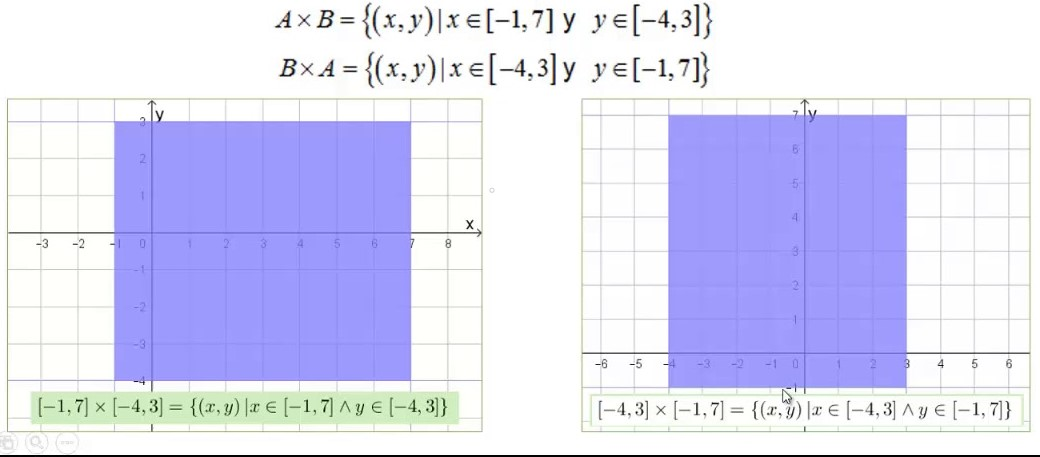
\includegraphics[scale=0.5]{producto cartesiano}
\end{center}
\end{defi}
 
\begin{defi}[Correspondencia]
Sean $A$ y $B$ conjuntos, definimos \textbf{una correspondencia entre ambos} como un $C\subset A \times B$ tal que $\forall a \in A : \exists! b \in B : (a,b)\in C$, es decir, un conjunto formado por pares ordenados en los que cada elemento de $A$ tiene un único elemento de $B$ asociado.
\end{defi}

\begin{obs}
La definición no obliga a que todo elemento tenga un correspondiente.
\end{obs}

\begin{defi}[Dominio y Rango]
Sea $C$ una correspondencia entre $A$ y $B$, definimos el \textbf{dominio de C} como los elementos que poseen un correspondiente en $B$, es decir:
$$dom(C)=\left\lbrace a\in A : \exists b \in B : (a,b)\in C\right\rbrace$$
Del mismo modo,  definimos el \textbf{rango o imagen de C} como los elementos de $B$ que están emparejados con algún elemento de $A$, es decir:
$$ran(C)=im(C)=\left\lbrace b\in B : \exists a \in A : (a,b)\in C\right\rbrace$$
\end{defi}

\begin{obs}
Si $C$ es una correspondencia entre $A$ y $B$ y $(x,y)\in C$, es habitual referirse a $y\in B$ como la imagen de $x \in A$. 
\end{obs}

\begin{defi}[Función]
Sea $C$ una correspondencia entre $A$ y $B$, la llamamos \textbf{función o aplicación} si y sólo si $dom(f)=A$, es decir, si todo elemento de $A$ tiene un correspondiente en $B$.
$$f: A\rightarrow B$$
\end{defi}

\begin{obs}
A los conjuntos $A$ y $B$ se los suele llamar dominio y codominio respectivamente, además las definiciones de elementos de las correspondencias se pueden reducir a:
$$dom(f)=\left\lbrace x \in A : \exists f(x)\in B\right\rbrace$$
$$ran(f)=im(f)=\left\lbrace y\in B : \exists x \in A : y=f(x)\right\rbrace$$
Además, si observamos como la función trata a conjuntos completos, vemos que:
$$E\subset A\Rightarrow f(E)=\{\forall b\in B : \exists a \in E : b=f(a)\}$$
$$F\subset B\Rightarrow f^{-1}(F)=\{a \in A : f(a)\in F\}$$
es decir, la condición de función al aplicarse a elementos también afecta a conjuntos.
\end{obs}

\begin{defi}[Inyectividad]
Sean $A$ y $B$ conjuntos y $f: A \rightarrow B$ una función entre ambos, decimos que $f$ es \textbf{inyectiva} cuando no hay elementos de $A$ con la misma imagen en $B$:
$$\forall a_1, a_2 \in A : a_1 \neq a_2\Rightarrow f(a_1)\neq f(a_2)$$
Para ello, es necesario que $card(A)\leq card(B)$
\end{defi}

\begin{obs}
En la práctica, para calcular si una función es inyectiva o no, tomaremos $f(x_1)=f(x_2)$ y si eso resulta en $x_1=x_2$ entonces es inyectiva, si no, no.

También se puede coger un elemento $y$ que pertenezca a la imagen, despejar $x$ de $y=f(x)$ y ver si para un mismo $y$ hay varios valores de $x$.
\end{obs}

\begin{ej}
Tomamos la función $f(x)=x^2$:
$$f(x_1)=f(x_2)\Rightarrow x_1^2=x_2^2\Rightarrow x_1^2-x_2^2=0 \Rightarrow$$
$$\Rightarrow (x_1-x_2)(x_1+x_2)=0 \Rightarrow
\begin{cases}
x_1-x_2=0 \Rightarrow & x_1=x_2 \\
x_1+x_2=0 \Rightarrow & x_1=-x_2 \\
\end{cases}
\Rightarrow \mbox{ no es inyectiva}$$
\end{ej}

\begin{ej}
Tomamos la función $f: \mathbb R^+ \rightarrow \mathbb R^+ : f(x)=\frac{x^2}{1+x}$:
$$y\in im(f)\Rightarrow y=f(x)=\frac{x^2}{1+x}\Leftrightarrow x^2-yx-y=0$$
$$x=\frac{y\pm \sqrt{y^2+4y}}{2}\mbox{ pero como }\frac{y\pm \sqrt{y^2+4y}}{2}<0\Rightarrow x\notin \mathbb R^+\Rightarrow inyectiva$$
\end{ej}

\begin{ej}
Supongamos estos dos conjuntos $E=\{x\in \mathbb R : 1\leq x\leq 2\}$, $G=\{y\in \mathbb R : 1\leq y\leq 4\}$ y la siguiente función $f(x)=\frac{1}{x^2}$, entonces:
$$f(E)?\rightarrow 1\leq x\leq 2\Leftrightarrow 1\leq x^2\leq 4\Leftrightarrow 1\geq x\geq \frac{1}{4}=f(E)$$
$$f^{-1}(G)?\rightarrow 1\leq y=f(x)=\frac{1}{x^2}\leq 4\Leftrightarrow 1\geq x^2\geq \frac{1}{4}\Leftrightarrow 1\geq |x|\geq \frac{1}{2} 
\begin{cases}
1\geq x\geq \frac{1}{2}& \Rightarrow 1\geq x\geq \frac{1}{2} \\
1\geq -x\geq \frac{1}{2}& \Rightarrow -1\leq x\leq -\frac{1}{2}
\end{cases}$$
\end{ej}

\begin{defi}[Suprayectividad]
Sean $A$ y $B$ conjuntos y $f: A \rightarrow B$ una función entre ambos, decimos que $f$ es \textbf{suprayectiva o sobreyectiva} cuando todos los elementos de $B$ son imágenes\footnote{Lo que se traduce en que $im(f)=B$} de algún elemento de $A$, es decir:
$$\forall b \in B : \exists a \in A : f(a)=b$$
Para ello, es necesario que $card(A)\geq card(B)$
\end{defi}

\begin{obs}
En la práctica, para calcular si una función es inyectiva o no, tomaremos $y=f(x)$ y despejaremos $x$, si $y$ toma como posibles valores los mismos que los valores del codominio, es suprayectiva.
\end{obs}

\begin{ej}
Tomamos la función $f(x)=x^2$:
$$y=x^2\Rightarrow x=\sqrt{y}\Rightarrow y\in (0,\infty)$$
Luego no es suprayectiva porque $f: \mathbb R \rightarrow \mathbb R$
\end{ej}

\begin{defi}[Biyectividad]
Sean $A$ y $B$ conjuntos y $f: A \rightarrow B$ una función entre ambos, decimos que $f$ es \textbf{biyectiva} cuando es inyectiva y suprayectiva simultáneamente.

Para ello, es necesario que $card(A) = card(B)$.
\end{defi}

\begin{obs}
No es difícil entre ver que la cantidad de elementos en los distintos conjuntos determinan en cierto modo (puesto que  para conjuntos infinitos no podemos contarlos) la obtención o no de los calificativos anteriores. De este hecho se desprende que:
$$\mbox{Sea }f: A\rightarrow B\mbox{ suprayectiva}\Rightarrow \exists f: B\rightarrow A \mbox{ inyectiva} $$
\end{obs}

\begin{defi}[Conjunto Numerable]
Sea $A$ un conjunto cualquiera, decimos que es \textbf{numerable}\footnote{Por ejemplo, $\mathbb R$ no es numerable} cuando existe una función biyectiva entre $\mathbb N$ y dicho conjunto.
\end{defi}


\begin{prop}
La unión numerable de conjuntos numerables es numerable:
$$\forall n\in \mathbb N : A_n\mbox{ es numerable}\Rightarrow \bigcup_{n\in \mathbb N} A_n\mbox{ es numerable}$$
El producto cartesiano de conjuntos numerables es numerable:
$$f:\mathbb N\stackrel{biyec.}{\rightarrow} \mathbb N \times \mathbb N \Rightarrow \mathbb N \times \mathbb N\mbox{ es numerable}$$
\begin{center}
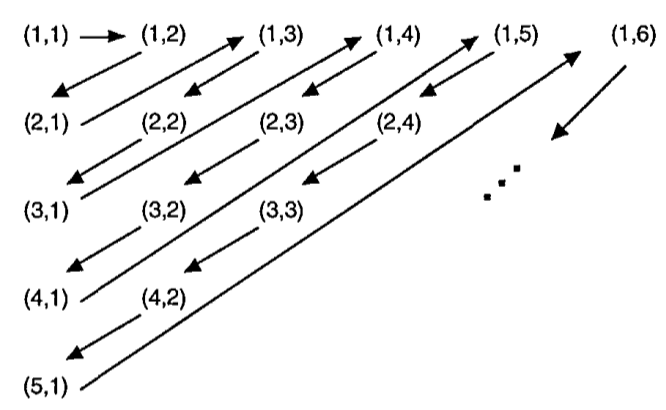
\includegraphics[scale=0.25]{nxn numerable}
\end{center}
\end{prop}

\begin{theo}[de Schöder-Berstein]
Sean $A$ y $B$ conjuntos, entonces:
$$\exists f: A\rightarrow B \mbox{ iny.}\mbox{ y } \exists g: A\rightarrow B \mbox{ supra. }\Rightarrow \exists h: A\rightarrow B \mbox{ biy.}$$
\end{theo}

\begin{defi}[Composición de funciones]
Sean $A$, $B$ y $C$ conjuntos y $f: A\rightarrow B$, $g: B\rightarrow C$ dos funciones, definimos la \textbf{composición de $f$ con $g$} como la función:
$$gof(a)=g\left(f(a)\right),\forall a \in A\Rightarrow gof: A\rightarrow C$$
\end{defi}

\begin{defi}[Conjunto $P(A)$]
Sea $A$ un conjunto, definimos el conjunto \textit{partes de A} como:
$$P(A) = \{D \subset A\}$$
es decir, aquel formado por todos los subconjuntos de $A$.
\end{defi}

\begin{ej}
Sea $A=\{a,b,c\}$, entonces $P(A)=\left\lbrace \{a\}, \{b\},\{c\}, \emptyset, \{a,b\}, \{a,c\}, \{b,c\}, A \right\rbrace$
\end{ej}

\begin{prop}
La función que relaciona $A$ con su $P(A)$ inyectiva.
\begin{eqnarray*}
f: A & \rightarrow & P(A)\mbox{ inyectiva}\Rightarrow card(A)\leq card(B)\\
a & \longmapsto  & \; \{a\}
\end{eqnarray*}
\end{prop}

\begin{obs}
Concretamente para el conjunto vacío:
$$A=\emptyset \Rightarrow P(A)=\{\emptyset\} \Rightarrow P(P(A))=\{\emptyset, \{\emptyset\}\}$$
\end{obs}

\begin{theo}[de Cantor]
Sea $A$ un conjunto cualquiera, entonces $\nexists f: A \rightarrow P(A)$  suprayectiva.
\end{theo}
\begin{demo}
Supongamos que sí:
\begin{eqnarray*}
\exists f: A &\rightarrow & P(A)\mbox{ suprayectiva} \\
x & \longmapsto & f(x)
\end{eqnarray*}
Sea el conjunto $D=\{ x\in A: x\notin f(x)\}$ como $D\subset A\Rightarrow D\in P(A)$ y como f es suprayectiva $\Rightarrow \exists a \in A : f(a)=D$
Llegados este punto:
\begin{itemize}
\item Si $a\in D\Rightarrow a\notin f(a)\mbox{ pero }f(a)=D \mbox{ \#}$
\item Si $a\notin D\Rightarrow a\in f(a)\mbox{ pero }f(a)=D \mbox{ \#}$
\end{itemize}

De este razonamiento se desprende que $\mathbb N$ es numerable pero $P(\mathbb N )$ no lo es puesto que ser biyectivo a $\mathbb N$ supondría la existencia de alguna aplicación suprayectiva y como hemos demostrado no es cierto.
\begin{itemize}
\item Usando el axioma de elección $\rightarrow card(P(\mathbb N))\leq card (\mathbb R)$
\item Usando la hipótesis del continuo $\rightarrow card(P(\mathbb N))= card (\mathbb R)$
\end{itemize}
\end{demo}

\subsection{Principio de Inducción}
En este pequeño espacio aparte, vamos estudiar el concepto de la inducción matemática. Este modo de demostración, fundamental y básico no sólo en esta asignatura, está presente en multitud de demostraciones importantes y es muy útil para demostrar enunciados que hagan referencia a cantidades discretas, en las que interviene algún elemento natural arbitrario.

Sea $\mathbb N=\{1, 2, 3,...\}$, este conjunto posee una propiedad que se llama de Buen Orden que dice:
$$A\subset \mathbb N, A\neq \emptyset \Rightarrow \exists m \in A : \forall a \in A : m\leq a$$
Lo que quiere decir que siempre encontraremos en ese subconjunto A un elemento que podremos calificar como el \textit{primero}.

\begin{theo}[Principio de Inducción]
Sea $S\subset \mathbb N$, entonces:
$$1\in S\wedge (k\in S\Rightarrow k+1\in S)\Rightarrow S=\mathbb N$$
\end{theo}
\begin{demo}
Supongamos que $S\subsetneq \mathbb N$ y que $A=\mathbb N\mbox{\textbackslash} S\neq 0$. Por la propiedad del Buen Orden:
$$\exists m \in A : \forall a \in A: m\leq a$$
Sin embargo, $m=1\notin A$ porque $1\in S$, luego $m-1\in S\stackrel{Hip. 2}{\Rightarrow} (m-1)+1=m\in S \mbox{ \#}$\par
O dicho de otra forma: si $1\in S\Rightarrow 2\in S \Rightarrow ... \Rightarrow \mathbb N=S\Rightarrow A=\mathbb N \mbox{\textbackslash} S=\mathbb N \mbox{\textbackslash} \mathbb N=\emptyset \mbox{ \#}$
\end{demo}

\begin{coro}
Supongamos que tenemos una propiedad que depende de un número natural: $k \in \mathbb N : P(k)$ y supongamos que $P(1)$ es cierto. Si $P(k)\Rightarrow P(k+1)$ entonces $\forall n \in \mathbb N : P(n)$.
\end{coro}
\begin{demo}
Supongamos el conjunto $S$
\begin{itemize}
\item $1\in S$
\item $k\in S\Rightarrow k+1\in S$
\end{itemize}
Los dos hechos anteriores según el principio de inducción implican que $S=\mathbb N\Rightarrow \forall n \in \mathbb N : P(n)$
\end{demo}

\chapter{Números Reales}
Los seres humanos a lo largo de la Historia han ido descubriendo distintos conjuntos útiles en función de las necesidades que iban surgiendo en cada momento. Hasta el momento, entre los fundamentales para este curso, tenemos:
$$\mathbb N\subset \mathbb Z\subset \mathbb Q\subset \mathbb R\subset \mathbb C$$
Donde entendemos cada conjunto como:
\begin{itemize}
\item $\mathbb N = \{1,2,3,4,...\}$ como el conjunto de los naturales
\item $\mathbb Z = \{..., -1, 0 ,1, ...\}$ como el conjunto de los enteros, formados por los naturales, el 0 y los negativos.
\item $\mathbb Q={\frac{a}{b}: a,b\in \mathbb Z \wedge b\neq 0}$ como el conjunto de los racionales en los que cada número racional está representado por un conjunto de fracciones equivalentes: $[\frac{a}{b}]={\frac{m}{n}: \frac{m}{n}=\frac{a}{b}}$.
\item $\mathbb{R}$ como el conjunto de los reales, formados por los irracionales y los racionales.
\end{itemize}

\section{Propiedades Algebraicas de $\mathbb R$}
Naturalmente, sin un conocimiento profundo de la estructura interna del cuerpo de los números reales y de las propiedades que tienen dichos números no podemos desarrollar un curso exhaustivo de análisis en variable real. Por tanto, en primer lugar, vamos a estudiar qué características tiene el cuerpo de los números reales y de qué forma interactúan con elementos matemáticos como desigualdades, valores absolutos, operaciones...

\subsection{Estructura de Cuerpo}
Las primeras propiedades a desarrollar van a ser las consecuencias directas de la estructura de cuerpo conmutativo y unitario que tiene el cuerpo de los números reales.

\begin{defi}[Suma]
Sea $\mathbb K$ un conjunto de números, definimos \textbf{la suma} como la operación interna que cumple las siguientes propiedades:
\begin{eqnarray*}
+: \mathbb K \times\mathbb K & \stackrel{+}{\rightarrow} & \mathbb K \\
(a,b) & \longmapsto  & a+b
\end{eqnarray*}
\begin{enumerate}
\item Propiedad conmutativa: $\forall a, b \in \mathbb K: a+b=b+a$
\item Propiedad asociativa: $\forall a, b, c\in \mathbb K : (a+b)+c=a+(b+c)$
\item Propiedad elemento neutro: $\exists 0_k\in \mathbb K : \forall a \in \mathbb K : a+0_k=0_k+a=a$
\item Propiedad elemento opuesto: $\forall a \in \mathbb K : \exists (-a) : a+(-a)=0_k$
\end{enumerate}
\end{defi}

\begin{obs}
La dupla $(\mathbb K, +)$ que verifica todas las propiedades recibe el nombre de grupo conmutativo. Algunos ejemplos son $\mathbb {Z, Q, R, C}$ porque se cumplen las 4 propiedades, pero $\mathbb N$ no puesto que cumplen solo las dos primeras.
\end{obs}


\begin{defi}[Producto]
Sea $\mathbb K$, definimos \textbf{el producto} como la operación interna que cumple las siguientes propiedades:
\begin{eqnarray*}
\cdot: \mathbb K \times\mathbb K & \stackrel{\cdot}{\rightarrow} & \mathbb K \\
(a,b) & \longmapsto  & a\cdot b
\end{eqnarray*}
\begin{enumerate}
\item Propiedad conmutativa: $\forall a, b \in \mathbb K: a\cdot b=b\cdot a$
\item Propiedad asociativa: $\forall a, b, c\in \mathbb K : (a\cdot b)\cdot c=a\cdot (b\cdot c)$
\item Propiedad elemento neutro: $\exists 1_k\in \mathbb K : \forall a \in \mathbb K : a\cdot 1_k=1_k\cdot a=a$
\item Propiedad elemento inverso: $\forall a \in \mathbb K : \exists a^{-1} : a\cdot a^{-1}=1_k$
\end{enumerate}
\end{defi}

\begin{obs}
La dupla $(\mathbb K, \cdot)$ que verifica todas las propiedades recibe el nombre de grupo conmutativo. Algunos ejemplos son $\mathbb {Q, R, C}$ porque cumplen las 4 propiedades, pero $\mathbb {N,Z}$ no puesto que cumplen solo las tres primeras.
\end{obs}

\begin{obs}
La propiedad que relaciona\footnote{Que se cumple en todos los conjuntos anteriores.} ambas operaciones es la \textbf{propiedad distributiva}:
\begin{enumerate}
\item[5.] $\forall a,b,c\in \mathbb K: a\cdot (b+c)=ab+ac$
\end{enumerate}
\end{obs}

\begin{defi}[Cuerpo Conmutativo]
Sean $(\mathbb K, +)$ y $(\mathbb K, \cdot)$ ambos grupos conmutativos en los que se cumple la propiedad distributiva, decimos que $(\mathbb K, +, \cdot)$ es un \textbf{cuerpo conmutativo}.
\end{defi}

\begin{prop}[Propiedades de Cuerpo Conmutativo]
Sea $(\mathbb K, +, \cdot)$ un cuerpo conmutativo, se cumplen las siguientes propiedades:
\begin{enumerate}
\item \textbf{El elemento neutro de la suma es único}.
\item \textbf{El elemento neutro del producto es único}. 
\item \textbf{Si $x+a=a\Rightarrow x=0$}\par 
\item \textbf{Si $a\neq 0\in \mathbb K \Rightarrow x\cdot a=a\Rightarrow x=1$}.
\item \textbf{El elemento opuesto de $x\in \mathbb K$ es único y en particular $-(-x)=x$}.
\item \textbf{El elemento inverso de $x\neq 0\in \mathbb K$ es único, en particular $(x^{-1})^{-1}$}.
\item \textbf{$\forall x\in \mathbb K: x\cdot 0=0$, por tanto, el 0 no tiene inverso}. 
\item \textbf{$\forall x\in \mathbb K : -x=(-1)\cdot x$}.
\item \textbf{Conocidos $a, b\in \mathbb{K}$, la ecuación $x+a=b$ tiene una única solución $x=b-a$}.
\item \textbf{Si $a\neq 0$, la ecuación $a\cdot x=b$ tiene una única solución: $x=\frac{b}{a}$}.
\item \textbf{Si $ab=ac \mbox{ y } a\neq 0 \Rightarrow b=c$}. 
\item \textbf{Si $ab=0\Rightarrow a=0 \mbox{ o } b=0$}.
\item \textbf{Si $a, b \neq 0 \Rightarrow \exists (ab)^{-1} = a^{-1}b^{-1}$}.
\end{enumerate}
\end{prop}
\begin{demo}
\begin{enumerate}
\item Supongamos que hay dos elementos neutros, $e, e'$:
 \begin{equation*}
 \begin{cases}
 e'+e=e & \mbox{si } e'\mbox{ es el elemento neutro} \\
 e'+e=e' & \mbox{si } e \mbox{ es el elemento neutro}
 \end{cases}
 \Rightarrow e=e'
 \end{equation*}
\item Supongamos que hay dos elementos neutros, $e, e'$:
 \begin{equation*}
 \begin{cases}
 e'\cdot e=e & \mbox{si } e'\mbox{ es el elemento neutro} \\
 e'\cdot e=e' & \mbox{si } e \mbox{ es el elemento neutro}
 \end{cases}
 \Rightarrow e=e'
 \end{equation*}
\item Supongamos que:
$$x+a=a\Leftrightarrow x+a+(-a)=a+(-a)\Leftrightarrow x+0=0 \Leftrightarrow x=0$$
\item Como $a\neq 0, \exists a^{-1}\in \mathbb K$ y entonces:
$$x\cdot a=a \Leftrightarrow x\cdot a \cdot a^{-1}=a\cdot a^{-1}\Leftrightarrow x\cdot 1=1 \Leftrightarrow x=1$$
\item Supongamos que $x_1, x_2$ son ambos opuestos de $x$:
$$x_1=0+x_1=(x_2+x)+x_1=x_2+(x+x_1)=x_2+0=x_2$$
\item Supongamos que $x_1, x_2$ son inversos de $x$ entonces:
$$x_1=1\cdot x_1=(x_2\cdot x)\cdot x_1=x_2\cdot (x\cdot x_1)=x_2\cdot 1=x_2$$
\item Supongamos que:
$$x=x\cdot 1=x\cdot (1+0)=x\cdot 1+ x\cdot 0=x+ x\cdot 0 \Rightarrow 0=x\cdot 0$$
\item Supongamos que:
$$0=x\cdot 0=x(1+(-1))=x+(-1)x \Rightarrow -x=(-1)x$$
\item Supongamos que:
$$x+a=b \Rightarrow (x+a)+(-a)=b+(-a)\Leftrightarrow x=b+(-a)=b-a$$
\item Supongamos que:
$$a\cdot x=b \Rightarrow a^{-1}(ax)=a^{-1}b \Rightarrow x=\frac{b}{a}$$
\item Supongamos que:
$$ab=ac \Leftrightarrow a^{-1}(ab)=a^{-1}(ac) \Leftrightarrow a^{-1}a\cdot b=a^{-1}a\cdot c \Leftrightarrow b=c$$
\item Supongamos que:
\begin{equation*}
\begin{cases}
a=0 & (a=0\vee b=0) \equiv V \\
a\neq 0 & \exists a^{-1}\in \mathbb K : a^{-1}(ab)=0\cdot a^{-1}\Leftrightarrow b=0\Rightarrow (a=0 \vee b=0)\equiv T
\end{cases} 
\end{equation*}
\item Para la primera parte, por la propiedad 12. si $ab=0\Rightarrow (a=0\vee b=0)\Leftrightarrow (a\neq 0 \wedge b\neq 0) \Rightarrow ab\neq 0$.

Demostrado que $ab\neq 0$, $ab\neq 0\Rightarrow \exists (ab)^{-1}$
$$(a^{-1}b^{-1})(ab)=a^{-1} a \cdot b^{-1} b=1 \Rightarrow (a^{-1}b^{-1})=(ab)^{-1}$$
\end{enumerate}
\end{demo}

\subsection{Propiedades de orden}
Además de ser un cuerpo, el conjunto de los números reales posee una ``relación de orden'' que se escribe como ``$\leq$'' intrínseca que dota de una serie de propiedades a dicho conjunto. Esta relación toma especial relevancia puesto que las desigualdades están muy presentes durante el resto del documento y un manejo adecuado de las mismas es esencial para entender las demostraciones posteriores.

\begin{defi}[Relación de Orden]
Sea $\leq$ una relación binaria de un conjunto $A$ en sí mismo, decimos que ésta es una \textbf{relación de orden} si y sólo si verifica las siguientes propiedades:
\begin{itemize}
\item \textbf{Propiedad Reflexiva}: $\forall x\in  A: x \leq x$
\item \textbf{Propiedad Antisimétrica}: $(x\leq y) \wedge (y\leq x) \Rightarrow x=y$
\item \textbf{Propiedad Transitiva}: $(x\leq y) \wedge (y \leq z) \Rightarrow x\leq z$
\item \textbf{Propiedad de Orden Total}: $\forall x,y\in A: (x\leq y) \vee (y\leq x)$
\end{itemize}
Si a un cuerpo $(\mathbb K, +, \cdot)$ se le agrega una relación de orden definidas como $\leq$ , decimos que se trata de un cuerpo \textbf{totalmente ordenado}. 
\end{defi}

\begin{obs}
Esta relación de orden tiene una serie de propiedades con respecto a las operaciones:
\begin{enumerate}
\item $x\leq y \Rightarrow \forall z \in \mathbb R : x+z\leq y+z$
\item $(x\geq 0 \wedge y \geq 0)\Rightarrow xy\geq 0$
\end{enumerate}
\end{obs}

\begin{defi}[Positividad y Negatividad]
Sea $x\in \mathbb{R}$ un número, decimos que dicho número es:
\begin{itemize}
\item \textbf{Positivo}: $ x> 0 \Leftrightarrow (0\leq x \mbox{ y } x\neq 0)$
\item \textbf{Negativo}: $ x < 0 \Leftrightarrow (-x)>0$
\end{itemize}
\end{defi}

\begin{prop}
En general, para cualquier cuerpo $(\mathbb K, +, \cdot)$ con relación de orden $\leq$ se verifica:
\begin{enumerate}
\item Si $(a>0) \wedge (b>0)\Rightarrow a+b>0$
\item Si $(a>0)\wedge (b>0)\Rightarrow ab>0$
\item Si $(a<0)\wedge (b<0)\Rightarrow ab>0$
\item Si $(a>0)\wedge (b<0)\Rightarrow ab<0$
\item Si $a,b\in \mathbb R$ decimos que $a>b\Leftrightarrow a-b>0$
\end{enumerate}
Concretamente en el contexto de $(\mathbb R, \leq)$, se cumplen además las siguientes propiedades:
\begin{enumerate}
\item Si $(a>b)\wedge (b>c)\Rightarrow a>c$
\item Si $a>b\Rightarrow a+x>b+x: \forall x\in \mathbb R$
\item Si $a\neq 0\Rightarrow a^2=a\cdot a>0$
\item \textbf{Tricotomía del Orden}: Si $a\in \mathbb R\Rightarrow (a>0)\vee (a<0)\vee (a=0)$
\item $1>0$
\item Si $(a>b) \wedge (c\geq d)\Rightarrow a+c>b+d$
\item Si $(a>b) \wedge (c>0)\Rightarrow ac>bc$
\item Si $(a>b)\wedge (c<0)\Rightarrow ac<bc$
\item Si $(a>0)\Rightarrow (a^{-1}>0)$
\item Si $a<b\Rightarrow a<\frac{a+b}{2}<b$\par
Concretamente, entre dos números reales distintos hay infinitos números reales. En particular, si $0<b\Rightarrow 0\leq \frac{b}{2}\leq b$ y en consecuencia, hay infinitos números positivos sin que ninguno de ellos sea "el más pequeño".
$$a<b\Rightarrow 2a<a+b \Rightarrow a<\frac{a+b}{2}\mbox{ pero también }a+b<2b\Rightarrow \frac{a+b}{2}<b \Rightarrow a<\frac{a+b}{2}<b$$
\item Si $0\leq a\leq \varepsilon: \forall \varepsilon>0 \Rightarrow a=0$
\item Si $ab>0\Rightarrow [(a>0)\wedge (b>0)]\vee [(a<0)\wedge (b<0)]$
\item Si $ab<0\Rightarrow [(a<0)\wedge (b>0)]\vee [(a>0)\wedge (b<0)]$
\item Si $(a>b>0)\wedge (c>d>0)\Rightarrow ac>bd$
\item Si $0<a<b\Rightarrow \forall n \in \mathbb N : (0<a^n<b^n)\wedge (0<\frac{1}{b}<\frac{1}{a})$
\item Si $(a>1)\Rightarrow (\frac{1}{a}<1)$ y si $(0<a<1)\Rightarrow (\frac{1}{a}>1)$
\end{enumerate}
\end{prop}
\begin{demo}
\begin{enumerate}
\item $$a>0\Rightarrow a\geq 0\Rightarrow a+b\geq b \stackrel{Trans}{\Rightarrow} a+b\geq b\geq 0 \Rightarrow a+b\geq 0$$
$$\mbox{Si } a+b=0 \Rightarrow 0\geq b\geq 0\Rightarrow b=0 \mbox{ \#}\Rightarrow a+b\neq 0 \Rightarrow a+b>0$$
\item $$(a\geq 0) \wedge (b\geq 0)\Rightarrow (a>0) \wedge (b>0) \Rightarrow ab\geq 0$$
$$\mbox{Si }ab=0\Rightarrow (a=0)\vee (b=0)\mbox{ \#}\Rightarrow ab\neq 0 \Rightarrow ab>0$$
\item $$(-a>0)\wedge (-b>0)\Rightarrow (-a)(-b)>0\Rightarrow (-1)a(-1)b=(-1)(-1)ab=ab>0$$
\item $$(a>0)\wedge(-b)>0\Rightarrow a(-b)>0\Leftrightarrow a(-1)b=(-1)ab=(-ab)>0\Rightarrow ab<0$$
\end{enumerate}

\begin{enumerate}
\item $$(a>b)\wedge (b>c)\Rightarrow (a\geq b)\wedge (b\geq c)\Rightarrow a\geq b \geq c\stackrel{Trans.}{\Rightarrow} a\geq c$$
$$\mbox{Si } a=c\Rightarrow (b\leq c) \wedge (c\leq b)\Rightarrow c=b\mbox{ \#}\Rightarrow a>c$$
\item $$a>b\Rightarrow a\geq b \Rightarrow a+x\geq b+x \Rightarrow a+x+(-x)\geq b+x+(-x)\Leftrightarrow a\geq b \mbox{ \#}\Rightarrow a+x>b+x$$
\item $$\begin{cases}
a\geq 0 \Rightarrow & a>0\Rightarrow a^2>0 \\
a\leq 0 \Rightarrow & a<0 \Rightarrow a^2>0
\end{cases}$$
\item $$\begin{cases}
a=0\Rightarrow & a=0 \\
a\geq 0 \Rightarrow & a>0 \\
a\leq 0 \Rightarrow & a<0 \\
\end{cases}$$
\item $$1=1\cdot 1>0 \mbox{ Porque el elemento neutro es positivo}$$
\item $$\mbox{Como } a>b\Rightarrow a+c>b+c\mbox{, y de modo paralelo: } c+b>d+b\mbox{. Luego: }\Rightarrow a+c>b+d$$
\item $$(a>b)\Rightarrow (a-b>0)\mbox{, y como } (c>0)\Rightarrow c(a-b)>0 \Rightarrow ac-bc>0\Rightarrow ac>bc$$
\item $$(a>b)\Rightarrow (a-b>0)\mbox{, y como }(-c)>0 \Rightarrow $$
$$\Rightarrow (-c)(a-b)>0 \Rightarrow (-1)c(a-b)>0\Rightarrow c(a-b)<0\Rightarrow ac-cb<0\Rightarrow ac<bc$$
\item $$a>0\Rightarrow \exists a^{-1}$$
$$a^{-1}<0\Rightarrow 1=a\cdot a^{-1}<0 \mbox{ \#}\Rightarrow a^{-1}>0$$
\item $$\mbox{Si }a\neq 0\Rightarrow a>0\Rightarrow a>\varepsilon=\frac{a}{2}>0\mbox{ \#}\Rightarrow a=0$$
\item $$\mbox{Tomamos }a\neq 0, b\neq 0\Rightarrow 
\begin{cases}
a>0 \Rightarrow b>0 & \mbox{Si fuese } b<0\Rightarrow ab<0 \mbox{ \#}\\
a<0 \Rightarrow b<0 & \mbox{Si fuese } b>0\Rightarrow ab<0 \mbox{ \#}
\end{cases}
$$
\item $$\mbox{Tomamos }a\neq 0, b\neq 0\Rightarrow 
\begin{cases}
a>0 \Rightarrow b<0 & \mbox{Si fuese } b>0\Rightarrow ab>0 \mbox{ \#}\\
a<0 \Rightarrow b>0 & \mbox{Si fuese } b<0\Rightarrow ab>0 \mbox{ \#}
\end{cases}
$$
\item $$
\begin{cases}
\mbox{Como } (a>b) \wedge (c>0)\Rightarrow ac>bc   \\
\mbox{Como } (c>d) \wedge (b>0)\Rightarrow bc>db   \\
\end{cases}
\Rightarrow ac>bd
$$
\item $$\mbox{Por la propiedad anterior }\Rightarrow a^2<b^2\Rightarrow a^3<b^3\stackrel{induccion}{\Rightarrow} a^n<b^n\Rightarrow a^{n+1}<b^{n+1}$$
$$a^{n+1}=a^n\cdot a<b^n\cdot a\Rightarrow b^n\cdot a\stackrel{?}{<}b^{n+1}\Rightarrow b^n\cdot a< b^n\cdot b \Rightarrow a<b \mbox{, QED}$$
$$\mbox{Si } \frac{1}{b}>\frac{1}{a}\Rightarrow a\geq b \mbox{ \#}\Rightarrow \frac{1}{a}>\frac{1}{b}$$
\item $$a>1\Rightarrow a^{-1}\cdot a>1\cdot a^{-1}\Rightarrow 1>\frac{1}{a}$$
$$(0<a<1)\Rightarrow a<1\Rightarrow a^{-1}\cdot a<1\cdot a^{-1}\Rightarrow 1<\frac{1}{a}$$
\end{enumerate}
\end{demo}

\begin{prop}
Los números naturales están contenidos en los enteros como los enteros positivos:
$$\forall n \in \mathbb N: n\geq 1 \mbox{ y } \mathbb N =\{n\in \mathbb Z: n\geq 1\}=\{n\in \mathbb Z : n>0\}$$
Y cualquier número entero entro otros dos consecutivos es necesariamente uno de esos:
$$\forall n,m\in \mathbb Z : n\leq m\leq n+1\Rightarrow m=n\mbox{ o } m=n+1$$
\end{prop}
\begin{demo}
\begin{enumerate}
\item Como $1\geq 0\Rightarrow 2\geq 1 \Rightarrow ...$, demostramos por inducción sobre n:\par
Sea $S=\{n\in \mathbb N: n\geq 1\}$, $1\in S$ porque $1\geq 1$ y como $1\geq 1\Rightarrow 2\geq 2$ entonces tenemos que para un elemento $k$ del conjunto, otro $k+1$ también pertenece a él, en consecuencia por el principio de inducción: $\mathbb N=S$\par
Ahora sea $m\in \mathbb Z: m>0$ probamos  que es natural:
$$m\notin \mathbb N \Rightarrow (-m)\in \mathbb N \Rightarrow (-m)\geq  1\mbox{ pero como }m>0 \mbox{ \#}\Rightarrow m\in \mathbb Z$$
\vspace{0.5cm}
\item Si $m\neq n$ y $m\neq n+1$, sea $k=m-n>0$:
$$k=m-n>0\Rightarrow k\in \mathbb N \mbox{ pero como }n\leq m \leq n+1\Rightarrow m-n<\leq 1 \Rightarrow k\leq 1$$
$$\mbox{ pero como }m\neq n+1\Rightarrow k\neq 1\Rightarrow k<1\mbox{ \# Por ser natural k }$$
\end{enumerate}
\end{demo}

\subsubsection{Desigualdades Notables}
Vamos a suponer demostrado (aunque lo haremos después) que si $a\in \mathbb R : a>0\Rightarrow \exists x\in \mathbb R : (x>0)\wedge (x^2=a)$

\begin{theo}[Discriminante en ecuaciones]
Sean $a,b,c\in \mathbb R  : a\neq 0$, la ecuación $ax^2+bx+c=0$ y el discriminante $\Delta=b^2-4ac$, entonces:
\begin{itemize}
\item Si $\Delta<0\Rightarrow \nexists x\in \mathbb R : ax^2+bx+c=0$
\item Si $\Delta>0 \Rightarrow \exists x\in \mathbb R : x=\frac{-b\pm\sqrt{\Delta}}{2a}$
\item Si $\Delta=0 \Rightarrow \exists! x\in \mathbb R : x=\frac{-b}{2a}$
\end{itemize}
\end{theo}
\begin{demo}
$$ax^2+bx+c=0\stackrel{a\neq 0}{\Leftrightarrow} x^2+\frac{bx}{a}+\frac{c}{a}=0\Leftrightarrow (x+\frac{b}{2a})^2-\frac{b^2}{4a^2}+\frac{c}{a}=0\Leftrightarrow (x+\frac{b}{2a})^2=\frac{\Delta}{4a^2}$$
\begin{itemize}
\item Si $\Delta>0\Rightarrow \mbox{ Q.E.D.}$
\item Si $\Delta<0\Rightarrow 0<(x+\frac{b}{2a})^2 \neq \frac{\Delta}{4a^2}<0$
\item Si $\Delta=0\Rightarrow x+\frac{b}{2a}=0\Rightarrow x=-\frac{b}{2a}$
\end{itemize}
\end{demo}

\begin{theo}[Discrimintante en inecuaciones]
Sean $a,b,c\in \mathbb R$ donde $a>0$, la inecuación $ax^2+bx+c\geq 0$ y el discriminante $\Delta=b^2-4ac$, entonces:
\begin{itemize}
\item Si $\Delta\leq 0\Rightarrow \forall x$ es cierto
\item Si $\Delta>0 \Rightarrow \exists x \in \mathbb R : x\geq \frac{-b\pm\sqrt{\Delta}}{2a} \wedge x\leq \frac{-b\pm\sqrt{\Delta}}{2a}$
\end{itemize}
\end{theo}
\begin{demo}
$$ax^2+bx+c\geq 0\stackrel{a\neq 0}{\Leftrightarrow} x^2+\frac{bx}{a}+\frac{c}{a}\geq 0\Leftrightarrow (x+\frac{b}{2a})^2-\frac{b^2}{4a^2}+\frac{c}{a}\geq 0\Leftrightarrow (x+\frac{b}{2a})^2\geq \frac{\Delta}{4a^2}$$
\begin{itemize}
\item Si $\Delta\leq 0\Rightarrow 0<(x+\frac{b}{2a})^2 \geq \frac{\Delta}{4a^2}<0$
\item Si $\Delta>0\Rightarrow (x+\frac{b}{2a})^2 \geq \frac{\Delta}{4a^2}\Leftrightarrow \left((x+\frac{b}{2a})+\sqrt{\frac{\Delta}{4a^2}}\right)\left((x+\frac{b}{2a})-\sqrt{\frac{\Delta}{4a^2}}\right)$
\end{itemize}
\end{demo}

\begin{theo}[Desigualdad de Cauchy]
Sea $n\in \mathbb N$ y $a_1, a_2, ..., a_n, b_1, b_2, ..., b_n\in \mathbb R$, entonces:
$$(a_1b_1+a_2b_2+...+a_nb_n)^2 \leq (a_1^2+...+a_n^2)\cdot (b_1^2+...+b_n^2)$$
Además, la igualdad sólo ocurre cuando:
$$\exists c\in \mathbb R : \forall i=1,...n :a_i=c\cdot b_i$$
\end{theo}
\begin{demo}
Sea $F(t)=(a_1-tb_1)^2+...+(a_n-tb_n)^2 : t\in \mathbb R$, se observa que la función siempre cumple que ``$\geq 0$'' por ser suma de cuadrados. Desarrollando los binomios\footnote{Llamamos a cada cosa con una letra mayúscula para simplificar la demostración}:
$$F(t)=\sum_{i=1}^n (a_i)^2 -2t\sum_{i=1}^n (a_ib_i) + t^2\sum_{i=1}^n (b_i)^2=A-2Ct+Bt^2$$
Para los casos\footnote{Es obvio que nunca puede ser menor que 0 pero para el caso $B=0\Rightarrow \forall i, b_i=0$ y se ve fácilmente en la fórmula inicial que eso siempre es cierto} en los que $B>0\Rightarrow$:
$$\Delta\leq 0\Leftrightarrow 4C^2-4AB\leq 0\Leftrightarrow 4C^2\leq 4AB\Leftrightarrow C^2\leq AB$$
De este modo se ve fácilmente que para el caso de $C^2=AB\Rightarrow \Delta=0\Rightarrow \exists c\in \mathbb R : F(c)=0\Rightarrow \forall  i, a_i-c\cdot b_i=0$
\end{demo}

\begin{theo}[Desigualdad de Minkovski]
Sea $n\in \mathbb N$ y $a_1, a_2, ..., a_n, b_1, b_2, ..., b_n\in \mathbb R$, entonces:
$$\sqrt{(a_1+b_1)^2+...+(a_n+b_n)^2}\leq \sqrt{a_1^2+...+a_n^2}+\sqrt{b_1^2+...+b_n^2}$$
Además, la igualdad sólo ocurre cuando:
$$\exists c\in \mathbb R : \forall i=1,...,n : a_i=c\cdot b_i$$
\end{theo}
\begin{demo}
$$\sum_{i=1}^n (a_i+b_i)^2=\sum_{i=1}^n (a_i)^2+2\sum_{i=1}^n (a_ib_i)+ \sum_{i=1}^n (b_i)^2\stackrel{Cauchy}{\leq}A+2\sqrt{A}\sqrt{B}+B=(\sqrt{A}+\sqrt{B})^2\Leftrightarrow$$
$$\Leftrightarrow \sqrt{\sum_{i=1}^n (a_i+b_i)^2}\leq \sqrt{A}+\sqrt{B}$$
Concretamente para que se de el caso ``='': $2\sum_{i=1}^n (a_ib_i)=2\sqrt{A}+\sqrt{B}$
\end{demo}

\subsection{Distancias y Valor Absoluto}
El concepto de distancia toma especial relevancia en apartados como la definición de límite, las sucesiones de Cauchy y otros elementos matemáticos que iremos viendo más adelante. Por ello, es muy útil recordar todos los enunciados relativos al valor absoluto (pues es la métrica que se emplea en $\mathbb{R}$).

\begin{defi}[Valor Absoluto]
Sea $a\in \mathbb R$, definimos la función \textbf{valor absoluto} como la función $|\cdot| : \mathbb{R}\rightarrow \mathbb{R}$ tal que:
$$
|a|=max\{a,-a\} =
\begin{cases}
a & a>0 \\
0 & a=0 \\
-a & a<0
\end{cases}
$$
\end{defi}

\begin{prop}[Propiedades del Valor Absoluto]
\begin{enumerate}
\item $|a|=0\Leftrightarrow a=0$
\item $|-a|=|a|: \forall a \in \mathbb R$
\item $|ab|=|a||b|: \forall a,b\in \mathbb R$
\item $\forall c\geq 0: |a|\leq c \Leftrightarrow -c\leq a\leq c$
\item $\forall a \in \mathbb R: -|a|\leq a\leq |a|$
\end{enumerate}
\end{prop}
\begin{demo}
\begin{enumerate}
\item Dada por la propia definición
\item Por definición: $max\{a,-a\}=max\{-a,-(-a)\}$
\item Para esta distinguimos casos:
	\begin{itemize}
	\item Para $a=0$ o $b=0$, es inmediata porque $|ab|=|a|\cdot |b|=0\cdot |b|=0$
	\item Para $a>0$, $b>0$ y $a,b\neq 0$: $|ab|=|a|\cdot |b|\Leftrightarrow ab=a\cdot b$
	\item Para $a<0$, $b<0$ y $a,b\neq 0$:$|ab|=|a|\cdot |b|\Leftrightarrow -ab=-a\cdot (-b)\Leftrightarrow ab=a\cdot b$
	\item Para $a>0$, $b<0$ y $a,b\neq 0$: $|ab|=|a|\cdot |b|\Leftrightarrow -ab=a\cdot(-b)$
	\end{itemize}

\item $|a|=max\{a,-a\}\leq c\Leftrightarrow a\leq c$ y $-a\leq c\Leftrightarrow a\leq c$ y $a\geq -c\Leftrightarrow -c\leq a\leq c$
\item Demostrada la propiedad 4. , se trata de decir que $c=a$
\end{enumerate}
\end{demo}

\begin{theo}[Desigualdad triangular]
Sean $a,b\in \mathbb R$ números reales, entonces:
$$|a+b|\leq|a|+|b|$$
\end{theo}
\begin{demo}
Tenemos que $-|a|\leq a\leq |a|$ y que $-|b|\leq b\leq |b|$, sumando ambas expresiones:
$$-|a|-|b|\leq a+b\leq |a|+|b|\Leftrightarrow -(|a|+|b|)\leq a+b\leq (|a|+|b|)$$
\end{demo}

\begin{coro}
Sean $a,b\in \mathbb{R}$ números reales, entonces:
\begin{enumerate}
\item $||a|-|b||\leq |a-b|$
\item $|a-b|\leq |a|+|b|$
\end{enumerate}
\end{coro}
\begin{demo}
\begin{enumerate}
\item Como $a=a-b+b\stackrel{Des.triang.}{\Rightarrow} |a|\leq |a-b|+|b|\Rightarrow |a|-|b|\leq |a-b|=c$.\par
Del mismo modo, $b=b-a+a\Rightarrow |b|\leq |b-a|+|a|\Rightarrow |b-a|=|a-b|\leq |b|-|a|\Rightarrow |a|-|b|\geq -|a-b|=-c$
$$||a|-|b||\leq c=|a-b|$$

\item $|a-b|=|a+(-b)|\leq |a|+|-b|=|a|+|b|$
\end{enumerate}
\end{demo}

\begin{defi}[Distancia entre números]
Sean $a,b\in \mathbb{R}$ números reales, definimos la \textbf{distancia entre $a$ y $b$} como:
$$dist(a,b)=|a-b|$$
dicha función conforma una métrica en $\mathbb{R}$.
\end{defi}

\begin{prop}[Propiedades de la Distancia]
\begin{enumerate}
\item $\forall x,y\in \mathbb R: d(x,y)\geq 0$ y $d(x,y)=0\Leftrightarrow x=y$

\item $\forall x,y\in \mathbb R: d(x,y)=d(y,x)$

\item Propiedad triangular: $\forall x,y,z\in \mathbb R : d(x,y)\leq d(x,z)+d(z,y)$
\end{enumerate}
\end{prop}
\begin{demo}
\begin{enumerate}
\item $d(x,y)=|x-y|\geq 0 : \forall x,y\in \mathbb R$

\item $d(x,y)=|x-y|=|y-x|=d(y,x)$

\item $d(x,y)=|x-y|=|x-z+z-y|\leq |x-z|+|z-y|=d(x,z)+d(z,y)$
\end{enumerate}
\end{demo}

\begin{defi}[Intervalos]
Sean $a,b\in \mathbb R$ donde $a<b$, definimos:
\begin{enumerate}
\item \textbf{Intervalo abierto}: $(a,b)=\{x\in \mathbb R: a<x<b\}$
\item \textbf{Intervalo cerrado}: $[a,b]=\{x\in \mathbb R: a\leq x\leq b\}$
\item \textbf{Intervalo semiabierto o semicerrado}: $[a,b)=\{x\in \mathbb R: a\leq x<b\}$ y viceversa.
\end{enumerate}
\end{defi}

\begin{obs}
El conjunto de los números reales se puede expresar como $\mathbb R=(-\infty,\infty)$ y se suele representar en lo que conocemos como \textbf{Recta Real}.
\end{obs}

\begin{defi}[Entornos]
Sea $a\in \mathbb{R}$ un número y $r\in \mathbb{R}$ una distancia, definimos un \textbf{entorno abierto} como el conjunto de números a distancia menor que $r$ de un número central $a$:
$$E(a,r)=\{x\in \mathbb R : dist(x,a)<r\}=\{x\in \mathbb R :|x-a|<r\}=\{x\in \mathbb R :a-r<x<a+r\}$$
Sea $a\in \mathbb{R}$ un número y $r\in \mathbb{R}$ una distancia, definimos un \textbf{entorno cerrado} como el conjunto de números a distancia menor o igual que $r$ de un número central $a$:
$$\bar{E}(a,r)=\{x\in \mathbb R : dist(x,a)\leq r\}=\{x\in \mathbb R :|x-a|\leq r\}=\{x\in \mathbb R :a-r\leq x\leq a+r\}$$
\end{defi}

\section{Números Complejos}
A pesar de que el curso es sobre el análisis real, viene bien conocer unas nociones básicas sobre el cuerpo de los números complejos y las propiedades del mismo. En esta sección, vamos a dar una definición simplificada del cuerpo $\mathbb{C}$ para poder entrar de lleno en las propiedades y enunciados propios de este espacio.

\begin{defi}[Cuerpo de los Números Complejos]
Sea $\mathbb C=\{a,b\in \mathbb R: (a,b\in \mathbb{R}^2)\}$, la operación $+: \mathbb{C}\times \mathbb{C}\rightarrow \mathbb{C}$ definida como $(a,b) + (c,d) = (a+c, b+d)$ y la operación $\cdot : \mathbb{C}\times \mathbb{C}\rightarrow \mathbb{C}$ definida como $(a,b)\cdot (c,d)=(ac-bd,ad+bc)$, definimos el \textbf{cuerpo de los números complejos} como la terna $(\mathbb{C}, +, \cdot)$ y es conmutativo.
\end{defi}

\begin{prop}[Suma de Complejos]
La operación $+: \mathbb{C}\times \mathbb{C} \rightarrow \mathbb{C}$ definida como:
$$(a,b)+(c,d)=(a+c,b+d)$$
posee las siguientes propiedades:
\begin{itemize}
\item Conmutativa: $(a,b)+(c,d)=(c,d)+(a,b)=(a+c,b+d)$
\item Asociativa: $\left((a,b)+(c,d)\right)+(e,f)=(a,b)+\left((c,d)+(e,f)\right)$
\item Elemento neutro: $(0,0)\rightarrow (a,b)+(0,0)=(a,b)$
\item Elemento opuesto: $(-a,-b)\rightarrow (a,b)+(-a,-b)=(0,0)$
\end{itemize}
En resumen, $(\mathbb C, +)$ es un \textbf{grupo conmutativo}.
\end{prop}

\begin{prop}[Producto de Complejos]
Si tenemos que $(a,b),(c,d)\in \mathbb C$, definida como:
$$(a,b)\cdot (c,d)=(ac-bd,ad+bc)$$
posee las siguientes propiedades
\begin{itemize}
\item Conmutativa: $(a,b)\cdot (c,d)=(c,d)\cdot (a,b)$
\item Asociativa: $\left((a,b)\cdot(c,d)\right)\cdot (e,f)=(a,b)\cdot \left((c,d)\cdot (e,f)\right)$
\item Elemento neutro: $(1,0)\rightarrow (a,b)\cdot (1,0)=(a,b)$
\item Elemento inverso: $(a,b)^{-1}\rightarrow (a,b)\neq 0\Rightarrow \exists (a,b)^{-1}\in \mathbb C: (a,b)\cdot (a,b)^{-1}=(1,0)$
\item Distributiva: $(a,b)[(c,d)\cdot(e,f)]=(a,b)\cdot (c,d)+(a,b)(e,f)$
\end{itemize}
En resumen, $(\mathbb C, \cdot)$ es un \textbf{grupo conmutativo}.
\end{prop}

\begin{prop}[Producto por un Escalar]
La operación $\cdot : \mathbb{C}\times \mathbb{R}\rightarrow \mathbb{C}$ definida como:
$$\lambda(a,b)=(\lambda a,\lambda b)$$
posee las siguientes propiedades:
\begin{itemize}
\item Conmutativa: $\lambda(a,b)=(a,b)\lambda$
\item Asociativa: $\lambda(\mu \cdot (a,b))=(\lambda\mu)\cdot (a,b)$
\item Elemento neutro: $1\cdot (a,b)=(a,b)$
\item Distributiva: $(\lambda+\mu)(a,b)=\lambda (a,b)+\mu (a,b)$\par
\item Distributiva: $\lambda[(a,b)+(c,d)]=\lambda(a,b)+\lambda(c,d)$
\end{itemize}
\end{prop}

\begin{obs}
Identificamos un número real $x\in \mathbb R$ con el número complejo $(x,0)\in \mathbb C$:
$$f: x\in \mathbb R \rightarrow (x,0)\in \mathbb C$$
por tanto, podemos decir que $\mathbb{R}\subset \mathbb{C}$.

La unidad fundamental de los complejos queda definida como $i$ y denota el número complejo $(0,1)\in \mathbb C$. Sin embargo, vemos que $i^2=(-1,0)\in \mathbb R$, de lo que nace la notación $i^2=-1\Rightarrow i=\sqrt{-1}$ más conocida como la unidad imaginaria mencionada anteriormente.

Si tenemos un número complejo cualquiera $(a,b)\in \mathbb C$ lo podemos escribir como $(a,b)=(a,0)+(0,b)=a(1,0)+b(0,1)$ con lo cual cualquier número complejo puede expresarse como:
$$(a,b)=a+bi$$
Donde $a$ constituye su parte real y $b$ se llama parte imaginaria.
\end{obs}

\begin{defi}[Módulo, Argumento y Conjugado]
Sea el número complejo $z=a+bi\in \mathbb C$, definimos el \textbf{módulo de $z$} como:
$$|z|=\sqrt{a^2+b^2}$$
Sea $\theta\in (0,2\pi]$ un número\footnote{En la representación bidimensional de $\mathbb{C}$, constituye el ángulo, con el eje x del plano, del vector que representa a $z$.} real, decimos que es el \textbf{argumento de $z\neq 0$} si y sólo si:
\begin{align*}
cos(\theta)=\frac{a}{|z|} & & sen(\theta)=\frac{b}{|z|}
\end{align*}
Sea el número complejo $z=a+bi\in \mathbb C$, definimos el \textbf{conjugado de $z$} como el número complejo $\bar{z}=a-bi$.
\end{defi}

\begin{prop}
\begin{itemize}
\item Si $\theta \in \mathbb R$, $e^{\theta\cdot i}=cos(\theta)+i\cdot sen(\theta)$

\item Si $x\in \mathbb R : x= x+0i\in \mathbb C$, el módulo de ese número real es su valor absoluto: $|x|$

\item Si $z=a+bi\in \mathbb C\Rightarrow |z|=0\Leftrightarrow z=0\Leftrightarrow a=0=b$

\item Si $z=a+bi\in \mathbb C$, entonces: $z\cdot \bar{z}=|z|^2$\par
En particular, $z\cdot (\frac{1}{|z|^2}\cdot \bar{z})=1$, siendo lo del paréntesis \textbf{su inverso}.

\item Si $\theta\in \mathbb R: |e^{i\theta}|=1$

\item Si $\alpha, \beta \in \mathbb R$, entonces: $e^{\alpha i}\cdot e^{\beta i}=e^{i(\alpha +\beta)}$

\item Si $z\in \mathbb C$, entonces: $z=|z|e^{i\theta}$ donde $\theta$ es un argumento de $z$ \textbf{(Forma polar)}.

\item Si $z, \omega \in \mathbb C$ y escribimos ambos como: $z=|z|e^{i\alpha}$ y $\omega=|\omega|e^{i\beta}$, entonces: $z\cdot \omega=|z|\cdot |\omega|\cdot e^{i(\alpha +\beta)}$\par
\end{itemize}
\end{prop}
\begin{demo}
\begin{enumerate}
\item $z\cdot \bar{z}=(a+bi)(a-bi)=a^2+b^2=|z|^2$
\item ya está
\item Desarrollo directo:
$$e^{i\cdot \alpha}\cdot e^{i\cdot \beta}=\left( cos(\alpha)+i\cdot sen(\alpha)\right) \left( cos(\beta)+ i\cdot sen(\beta)\right)=$$
$$=\left( cos(\alpha)cos(\beta)-sen(\alpha)sen(\beta)\right)\cdot i\left( cos(\alpha)sen(\beta)+sen(\alpha)cos(\beta)\right)=$$
$$cos(\alpha + \beta)+ i\cdot sen(\alpha + \beta)= e^{i\cdot(\alpha + \beta)}$$

\item El argumento de $z$ verifica que $cos(\theta)=\frac{a}{|z|}$ y $sen(\theta)=\frac{b}{|z|}$, lo que verifica que $a=|z|cos(\theta)$ y $b=|z|sen(\theta)$, con lo cual: $z=a+bi=|z|(cos(\theta)+sen(\theta)\cdot i)=|z|e^{i\theta}$

\item $z=|z|e^{i\alpha}$ y $\omega=|\omega|e^{i\beta}$, entonces: $z\cdot \omega=|z|e^{i\alpha}\cdot |\omega|e^{i\beta}=|z|\cdot |\omega|\cdot e^{i(\alpha +\beta)}$
\end{enumerate}
\end{demo}

\begin{defi}[Exponencial compleja]
Sea $z=a+bi\in \mathbb C$, definimos la \textbf{exponencial compleja} como:
$$e^z = e^{a+bi}=e^a\cdot e^{bi}=e^a\cdot (cos(b)+i\cdot sen(b))=e^a\cdot cos(b)+e^a\cdot i\cdot sen(b)$$
Concretamente, cuando $z\in \mathbb{R}$, es decir, $b=0$:
$$e^a\cdot cos(b)+e^a\cdot i\cdot sen(b)=e^a$$
\end{defi}

\begin{obs}
A modo de recopilación de los enunciados anteriores, hay 4 formas de representar un número complejo:
\begin{itemize}
\item Forma binomial: $a+bi$
\item Forma trigonométrica: $|z|cos(\theta)+ |z|sen(\theta)i$
\item Forma polar: $|z|_\theta$
\item Forma exponencial: $z=|z|\cdot e^{\theta\cdot i}$
\end{itemize}
\end{obs}

\subsection{Teorema Fundamental del Álgebra}
Supongamos que tenemos un polinomio $P(z)$ con coeficientes complejos, decimos que el número $z_0\in \mathbb C$ es raíz de $P(z)$ lo que es equivalente a decir que: $P(z)=(z-z_0)Q(z)$.\par
Decimos que $z_0$ es raíz de $P(z)$ con multiplicidad $m\in \mathbb N\Leftrightarrow P(z)=(z-z_0)^mQ(z)$, donde $Q(z_0)\neq 0$.\par
El teorema dice que si tenemos un polinomio cualquiera de coeficientes complejos, siempre existe una raíz al menos.
$$f(x)\in \mathbb C[x]\Rightarrow \exists z_0\in \mathbb C: P(z_0)=0$$
Como consecuencia de dicho Teorema, si tenemos un polinomio $P(z)=a_nz^n+a_{n-1}z^{n-1}+\cdots + a_1z+a_0: a_0,\cdots, a_n\in \mathbb C \wedge a_n\neq 0$, entonces $P(z)$ tiene $n$ raíces complejas (teniendo en cuenta su multiplicidad). Es decir, $\exists z_0,\cdots, z_k\in \mathbb C$ y $\exists m_0,\cdots, m_k\in \mathbb N$, tales que $\sum_{i=1}^k(m_i)=n$ y tales que:
$$P(z)=a_n(z-z_1)^{m_1}\cdots (z-z_k)^{m^k}$$

\subsubsection{Raíces de números complejos}
Sea $z\in \mathbb C$ y $n\in \mathbb N$ buscamos $\omega \in \mathbb C: \omega^n=z$. Con lo cual para poder buscarlo, sabemos que buscamos un omega tal que:
$$\omega=r\cdot e^{i\theta}\mbox{ donde }r=|\omega|, \theta=argumento$$
De aquí se sigue que:
$$\omega^n=r^n\cdot e^{in\theta}=z=|z|\cdot e^{i\alpha}\Rightarrow
\begin{cases}
r^n=z & \Rightarrow r=\sqrt[n]{z} \\
e^{in\theta}=e^{i\alpha} & \Rightarrow n\theta=\alpha\Rightarrow \theta=\frac{\alpha+2\pi k}{n}
\end{cases}
$$
Donde $k=0,1,..., n-1$

\section{Supremos e Ínfimos}
En esta sección vamos a definir qué significa estar acotado y cuáles son las mejores cotas para un conjunto, es decir, cuál es el valor que representa mejor la ``barrera'' entre el conjunto en cuestión y el resto de $\mathbb{R}$. Este concepto es central y esencial en la asignatura pues interviene en absolutamente el resto de temas del curso.

\begin{defi}[Cotas]
Sea $A\subset R: A\neq \emptyset$, decimos que:
\begin{itemize}
\item $M\in R$ es \textbf{cota superior} de A si y sólo si $\forall a\in A: a\leq M$.

\item $m\in \mathbb R$ es \textbf{cota inferior} de A si y sólo si $\forall a\in A: m\leq a$.
\end{itemize}
Si $A$ posee cota superior o inferior decimos que está \textbf{acotado superiormente} o \textbf{acotado inferiormente} respectivamente.
\end{defi}

\begin{defi}[Ínfimos y Supremos]
Sea $A\subset R: A\neq \emptyset$, decimos que:
\begin{itemize}
\item $S\in \mathbb R$ es \textbf{supremo} de A si y sólo si $\forall M\in \mathbb R: S\leq M $, siendo $M$ cota superior.

\item $s\in \mathbb R$ es \textbf{ínfimo} de A si y sólo si $\forall m\in \mathbb R: m\leq s$, siendo $m$ cota inferior.
\end{itemize}
Además, si $\sup A \in A$ lo llamamos \textbf{máximo} y $\inf A \in A$ lo llamamos \textbf{mínimo}.
\end{defi}

\begin{theo}[Propiedad del Supremo]
Sea $A\subset \mathbb R: A\neq \emptyset$ un conjunto acotado superiormente, entonces existe el supremo.
\end{theo}

\begin{obs}
En los $\mathbb Q$ no es cierto y es la diferencia fundamental de este cuerpo con respecto a los $\mathbb R$, porque par el conjunto: $\{x\in \mathbb Q: x^2 < 2\}$, existe el supremo en $\mathbb R$, pero no en $\mathbb Q$.
\end{obs}

\begin{prop}
Sea $A\subset \mathbb R: A\neq \emptyset$ un conjunto acotado superiormente, el número $S\in \mathbb R$ es supremo si y sólo si:
\begin{enumerate}
\item Es único.
\item Es cota superior de A
\item $\forall y\in \mathbb R: y<S\Rightarrow \exists a\in \mathbb A: y<a\leq S$.
\item $\forall \varepsilon>0: \exists a\in A: S- \varepsilon <a\leq S$.
\end{enumerate}
\end{prop}
\begin{demo}
\begin{enumerate}
\item Demostramos la unicidad:\par
Supongamos que $S_1\neq S_2$ son ambos supremos de A, luego $S_1<S_2$ o $S_1>S_2$. Si suponemos\footnote{Al revés es igual} que $S_1<S_2$, como $S_1$ es cota superior de A y $S_2$ es supremo, $S_2\leq S_1$ \#.

\item Es por definición

\item Demostramos la doble implicación:
	\begin{itemize}
	\item ``$\Rightarrow$'':\par
	Sea $y\in \mathbb R: y<S$, supongamos que no existe:
	$$\forall a \in A: a\leq y \vee S<a\Rightarrow \mbox{como S es cota superior}\Rightarrow a\leq y\Rightarrow y \mbox{ es cota superior \#}$$
	Porque si $y$ es cota superior, $S\leq y$ luego absurdo.
	
	\item ``$\Leftarrow$'':\par
	Sea $M\in \mathbb R$ una cota superior de A, suponemos lo contrario a que $S\leq M$:\par
	Si $M<S\Rightarrow \exists a\in A: M<a\leq S$ \#, porque si $M$ es cota superior, no puede haber ningún elemento de A que sea mayor que él.
	\end{itemize}
	
\item Supongamos que no: $\forall a \in A: a<S-\varepsilon \vee S< a$. Si $S<a\Rightarrow S$ no es supremo, por lo tanto \# y si $S-\varepsilon> a: \forall a \in A\Rightarrow S-\varepsilon$ es supremo \#
\end{enumerate}
\end{demo}

\begin{prop}
Sea $A\subset \mathbb R: A\neq \emptyset$ un conjunto acotado inferiormente, el número $s\in \mathbb R$ es ínfimo si y sólo si:
\begin{enumerate}
\item Es único.
\item Es cota inferior de A
\item $\forall y\in \mathbb R: s<y\Rightarrow \exists a\in \mathbb A: s\leq a<y$.
\item $\forall \varepsilon>0: \exists a\in A: s\leq a<s+\varepsilon$.
\end{enumerate}
\end{prop}
\begin{demo}
\begin{enumerate}
\item Demostramos la unicidad:\par
Si $s_1\neq s_2$ son ínfimos, entonces $s_1<s_2$ o al revés pero la demostración es igual. Si $s_1<s_2$ como $s_2$ es cota inferior y $s_1$ es ínfimo: $s_2\leq s_1$ \#

\item Demostramos la doble implicación:
	\begin{itemize}
	\item ``$\Rightarrow$'':\par
	Sea $y\in \mathbb R: s<y$, si suponemos que no existe, entonces: $\forall a \in  A: a<s\vee y\leq a\Rightarrow\mbox{como s es cota inferior }\Rightarrow  y\leq a\Rightarrow y$ es cota inferior de A $\Rightarrow y\leq s$ \#.
	\item ``$\Leftarrow$'':\par
	Sea $m\in \mathbb R$ una cota inferior de A, suponemos lo contrario a que $s\geq m$:\par
	Sea $m$ cota inferior de A, si $s<m\Rightarrow \exists a\in A: s\leq a<m$ \#, porque $m$ es cota inferior.
	\end{itemize}
	
\item Suponemos que:
$$\exists m\in \mathbb R: m\leq a: \forall a\in A\Leftrightarrow -m\geq -a\Leftrightarrow -m\mbox{ es cota superior de B}=\{-a: a\in A\}\neq \emptyset$$
$$\Rightarrow \exists S\mbox{ supremo de B}: -a\leq S\Rightarrow a\geq -S$$
Aquí vemos que $-S$ es el ínfimo de A porque $-S$ es cota inferior de A y probamos que además es la mayor de las cotas inferiores, es decir, probamos $m\leq -S$:\par
Sea $m$ una cota inferior de A, $m\leq -S$, porque si no lo fuese:
$-S<m\leq a\Rightarrow S>-m\geq -a\Rightarrow -m$ es cota superior de B, \# porque $S$ es el supremo de B.
\end{enumerate}
\end{demo}

\begin{obs}
Sea $A\subset \mathbb R: A\neq \emptyset$ un conjunto no acotado, entonces lo denotamos de esta forma $sup(A)=+\infty$ y $inf(A)=-\infty$.
\end{obs}

\begin{theo}[de la existencia de raíces]
Sea $a\in \mathbb R: a>0$ y $n\in \mathbb N: n\geq 2$, entonces $\exists! r>0: r^n=a$.
\end{theo}
\begin{demo}
\begin{enumerate}
\item Demostramos primero la unicidad:\par
Supongamos que hay 2: $r_1\neq r_2$, podemos suponer entonces que: $r_1<r_2\Rightarrow r_1^n<r_2^n$ \# porque $a<a$ es absurdo.

\item Demostramos la existencia:\par 
Definimos el conjunto $A=\{x>0: x^n\leq a\}$, demostramos que $A\neq \emptyset$
$$\frac{a}{1+a}<a\mbox{ y del mismo modo: }\frac{a}{1+a}<1\Rightarrow \left(\frac{a}{1+a}\right)^n<\frac{a}{1+a}<a\Rightarrow \frac{a}{1+a}\in A$$
Ahora vemos que $A$ es acotado superiormente, para ello distinguimos dos casos:
	\begin{itemize}
	\item $a\leq 1\Rightarrow M=1$ es una cota superior de $A$ porque si no lo fuese:
$$\exists x\in A: x>1\Rightarrow x^n>1\geq a\Rightarrow \mbox{ \#}$$

	\item  $a>1\Rightarrow M=a$ es cota superior de $A$, porque si no lo fuese:
$$\exists x\in A: x>a>1 \Rightarrow x^n>a^n>a\Rightarrow\mbox{ \#}$$
	\end{itemize}

Al estar acotado superiormente, por la propiedad de supremo entonces: $\exists r=sup(A)>0$.
\item Queda solo demostrar $r^n=a$, para ello suponemos que $r^n<a$ y que $r^n>a$ y en ambos casos debemos llegar a una contradicción.
	\begin{itemize}
	\item Caso: $r^n<a\Rightarrow \exists h>0: (r+h)^n<a$, donde cogemos un $0<h<1$:
	
$$(r+h)^n=r^n+\sum_{j=0}^{n-1}\binom{n}{j}r^jh^{n-j}=r^n+h\sum_{j=0}^{n-1}\binom{n}{j}r^jh^{n-j-1}\stackrel{h^x<1}{\leq}r^n+h\sum_{j=0}^{n-1}\binom{n}{j}r^j=$$
$$=r^n+h\left[(r+1)^n-r^n\right]$$

\footnote{$\sum_{j=0}^{n-1}\binom{n}{j}r^j=\left[(r+1)^n-r^n\right]$, despejando el sumatorio de la expresión: $(r+h)^n=r^n+\sum_{j=0}^{n-1}\binom{n}{j}r^jh^{n-j}$, cuando $h=1$}

Ahora buscamos un $h$ que satisfaga:
$$r^n+h\left[(r+1)^n-r^n\right] <a \Rightarrow h<\frac{a-r^n}{(r+1)^n-r^n}$$
Luego puedo elegir un $0<h<\frac{a-r^n}{(r+1)^n-r^n}$ y $h<1$, porque entre dos positivos hay infinitos números.\par
Como existe dicho valor de $h$, llegamos a una contradicción porque que $(r+h)^n<a$ implica que $r+h\in A$, pero no puede ser porque $r$ es el supremo del conjunto y $r+h>r>x\in A=r+h\Rightarrow$ \#.
\vspace{0.5cm}
	\item Caso: $r^n>a\Rightarrow \exists h>0: (r-h)^n>a$, tratamos ahora de demostrar por reducción al absurdo que $r-h$ es una cota superior, para llegar a una contradicción:
$$\exists x\in A: x>r-h\Rightarrow x^n\geq (r-h)^n\Rightarrow a\geq x^n\geq (r-h)^n>a$$

Para que dicha contradicción sea posible es necesario verificar que existe algún valor de $h$ que verifica lo anterior, por lo que tomamos un $h: 0<h<1$, entonces:
$$(r-h)^n=r^n+\sum_{j=0}^{n-1}\binom{n}{j}r^j(-h)^{n-j}=r^n+h\sum_{j=0}^{n-1}\binom{n}{j}r^j(-1)^{n-j}h^{n-j-1}\geq $$
$$\stackrel{\mbox{\scriptsize{todos }}-}{\geq} r^n-h\sum_{j=0}^{n-1}\binom{n}{j}r^j h^{n-j-1}\stackrel{h=1\mbox{ \scriptsize{resta más}}}{\geq} r^n-h\sum_{j=0}^{n-1}\binom{n}{j}r^j=r^n-h\left[(r+1)^n-r^n\right]$$

Ahora buscamos un $h$ que satisfaga lo anterior:
$$r^n-h\left[(r+1)^n-r^n\right]>a\Leftrightarrow r^n-a>h\left[(r+1)^n-r^n\right]\Leftrightarrow 0<h<\frac{r^n-a}{(r+1)^n-r^n}\mbox{ donde } h\leq 1$$
Por lo que al poder encontrar un $h$ que satisfaga dicha expresión llegamos a una contradicción porque que $(r-h)^n>a$ implica que $r-h$ es cota superior de A, pero no puede ser porque $r$ es el supremo del conjunto y $r-h$ sería una cota superior, inferior al supremo $r$.
\end{itemize}
\end{enumerate}
\end{demo}

\begin{prop}
Sea $A\subset \mathbb{R}$ un conjunto real y $S\subset A$ un subconjunto suyo, entonces:
\begin{align*}
\sup S\leq \sup A && \inf S\geq \inf A
\end{align*}
\end{prop}


\subsection{Densidad de $\mathbb{Q}$ en $\mathbb{R}$}
Gracias a las propiedades del supremos y del ínfimo, vamos a demostrar que para cualquier número real que escojamos podemos encontrar un racional y un irracional tan cerca como queramos de dicho número. A esta propiedad se la conoce como densidad.

\begin{theo}[Propiedad Arquimediana de $\mathbb R$]
Para todo $x\in \mathbb R$ positivo, entonces $\exists n\in \mathbb N: x<n$, es decir, $\mathbb N$ no está acotado superiormente.
\end{theo}
\begin{demo}
Supongamos lo contrario, $\exists x>0\in \mathbb R: n\leq x: \forall n \in \mathbb N\Rightarrow \exists S=sup(\mathbb N)$, entonces por ser supremo: $\exists m \in \mathbb N : S-1<m\leq S\Rightarrow S<m+1$, pero como $m+1\in \mathbb N$ es absurdo.
\end{demo}

\begin{theo}[Propiedad Arquimediana del producto]
Sean $x,y\in \mathbb{R} : x>1, \ y>0$, entonces $\exists n\in \mathbb N: x^n > y$, incluso:
$$\forall x,y \in \mathbb{R} : y>0, \ x>1: \exists! n\in\mathbb N: x^n<y\leq x^{n+1}$$
\end{theo}
\begin{demo}
Supongamos que no:
$$\exists y>0, x>1: \forall n\in \mathbb N: y>x^n\Rightarrow\{x^n\}\mbox{ es acotado sup.}\Rightarrow \exists \sup=S\Rightarrow S-\varepsilon< x^m\leq S: \forall \varepsilon>0:\exists m\in \mathbb N\Rightarrow$$

Si soy capaz de encontrar un epsilon que verifique que $x^m+\varepsilon<x^{m+1}$ entonces ya tendría una contradicción porque como $S<x^m+\varepsilon< x^{m+1}$ tendríamos una potencia que sería mayor que el supremo.

$$\Rightarrow S< x^m +\varepsilon <x^{m+1}\Rightarrow \varepsilon<x^{m+1}(x-1)$$
Si escogemos un $\varepsilon< x-1\Rightarrow \varepsilon>0$ entonces lo anterior se verifica, así que como sí que existe un $\varepsilon$ positivo que cumple que $x^m+\varepsilon< x^{m+1}$ tenemos una contradicción.
\end{demo}

\begin{prop}
\begin{enumerate}
\item Si $x<0\in \mathbb R\Rightarrow \exists m\in \mathbb Z: m<x$, es decir, que $\mathbb Z$ no está acotado inferiormente.
\item Si $x,y\in \mathbb R: x,y>0\Rightarrow \exists n \in \mathbb N : y<nx$.
\item Si $x>0\Rightarrow \exists n \in \mathbb N : \frac{1}{n}<x$
\item Si $x>0$, entonces $inf\{\frac{x}{n}: n\in \mathbb N\}=0$
\item Si $x<0$, entonces $sup\{\frac{x}{n}: n\in \mathbb N\}=0$
\item Si $x>0\in \mathbb R\Rightarrow \exists! n \in \mathbb N: n-1\leq x< n$, es decir, en otras palabras\footnote{Y además dichos conjuntos son disjuntos dos a dos.}:
$$[0,\infty)=\bigcup_{n\in \mathbb N}[n-1,n)$$
\item Análogamente, si $x>0$, entonces $\exists! n \in \mathbb N: n-1< x\leq n$, es decir, en otras palabras\footnote{Y además dichos conjuntos son disjuntos dos a dos.}:
$$(0,\infty)=\bigcup_{n\in \mathbb N}(n-1,n]$$
\item Si $x\in \mathbb R\Rightarrow \exists! m \in \mathbb Z: m-1\leq x < m$, en otras palabras:
$$\mathbb R =\bigcup_{m\in \mathbb Z}[m-1,m)$$
\item Análogamente, si $x\in \mathbb R\Rightarrow \exists! m \in \mathbb Z: m-1< x\leq m$, en otras palabras:
$$\mathbb R =\bigcup_{m\in \mathbb Z}(m-1,m]$$
\item Si $x>0$ y $y\in \mathbb R\Rightarrow \exists! m \in \mathbb Z: (m-1)x\leq y <mx$, es decir, en otras palabras:
$$\mathbb R= \bigcup_{m\in \mathbb Z}[(m-1)x, mx)$$
\item Análogamente, si $x>0$ y $y\in \mathbb R\Rightarrow \exists! m \in \mathbb Z: (m-1)x< y \leq mx$, es decir, en otras palabras:
$$\mathbb R= \bigcup_{m\in \mathbb Z}((m-1)x, mx]$$
\end{enumerate}
\end{prop}
\begin{demo}
\begin{enumerate}
\item $$x<0\Rightarrow -x>0\stackrel{P.A.}{\Rightarrow} \exists n \in \mathbb N: -x<n\Leftrightarrow x>-n\in \mathbb Z$$
\item $$\frac{y}{x}>0\stackrel{P.A.}{\Rightarrow} \exists n \in \mathbb N : \frac{y}{x}<n \Leftrightarrow y<nx$$
\item $$\frac{1}{x}>0\stackrel{P.A.}{\Rightarrow }\exists n \in \mathbb N : \frac{1}{x}<n\Leftrightarrow x>\frac{1}{n}$$			
\item $$\mbox{0 es cota inferior de } \left\lbrace\frac{x}{n}: n\in \mathbb N\right\rbrace=A\Rightarrow 0\leq \frac{x}{n}: \forall n\in \mathbb N \Rightarrow \exists inf(A)=s\geq 0$$
$$\mbox{Si }s>0\Rightarrow 0<s\leq \frac{x}{n}\Leftrightarrow n\leq \frac{x}{s}\Rightarrow \mbox{ \# porque los naturales no tiene cota superior}$$
\item $$\mbox{0 es cota superior de } \left\lbrace\frac{x}{n}: n\in \mathbb N\right\rbrace=A\Rightarrow 0\geq \frac{x}{n}: \forall n\in \mathbb N\Rightarrow \exists sup(A)=S \leq 0$$
$$\mbox{Si }S<0\Rightarrow S\geq \frac{x}{n}\Rightarrow \frac{x}{S}\geq n: \forall n \in \mathbb N\Rightarrow \mbox{ \# porque los naturales no tiene cota superior}$$
\item Si $x>0$, sea $A=\{m\in \mathbb N: x<m\}\neq \emptyset$, entonces por la propiedad de Buen Orden, A tiene un primer elemento definido como $n\in A$, que implica que $x<n$
$$\begin{cases}n=1 &\Rightarrow 0\leq x<1=n\\
n\neq 1 &\Rightarrow n-1\notin A\Leftrightarrow n-1\leq x< n\end{cases}$$
Ahora demostramos la unicidad:
$$k\in \mathbb N: k-1\leq x<k\Rightarrow \begin{cases}k-1 \notin A \\ k \in A\end{cases}\Rightarrow k \mbox{ es el primer elemento}\Rightarrow k=n$$
Ahora demostramos la doble inclusión para demostrar que la unión de esos intervalos es el otro:
	\begin{itemize}
	\item ``$\supset$''
	$$\forall n \in \mathbb N: [n-1,n)\subset [0,\infty)\Leftrightarrow \bigcup_{n\in \mathbb N}[n-1,n) \subset [0,\infty)$$
	
	\item ``$\subset$''
	$$x\geq 0\Rightarrow \begin{cases} x=0 & \Rightarrow x\in [0,1) \\ x>0 & \Rightarrow \exists! n \in \mathbb N : [n-1,n)	
	\end{cases}\Rightarrow x\in \bigcup_{n\in \mathbb N}[n-1,n) $$
	\end{itemize}

Por último hay que ver que son disjuntos dos a dos:
$$n,m\in \mathbb N: n\neq m\Rightarrow n<m\Rightarrow n+1\leq m\Rightarrow n\leq m-1\Rightarrow [n-1,n)\cap [m-1,m)\neq \emptyset$$
Esto es así porque $x\in [n-1,n)\Rightarrow x<n$ y $x\in [m-1,m)\Rightarrow x\geq m+1$, todo implica que $m-1<n$ \#
\item Análoga a la anterior.
\item $$x\geq 0\Rightarrow \exists! n \in \mathbb N : n-1\leq x<n$$
$$x<0\Rightarrow -x>0 \Rightarrow \exists! n \in \mathbb N: n-1<-x\leq n\Leftrightarrow -n\leq x< -(n-1)\Leftrightarrow m-1=-n\leq x< -n+1=m$$
El resto de la demostración es como en los puntos anteriores
\item Igual que antes
\item $$\frac{y}{x}\in \mathbb R\Rightarrow \exists! m \in \mathbb Z: m-1\leq \frac{y}{x}< m\Rightarrow (m-1)x\leq y< mx$$
\end{enumerate}
\end{demo}

\begin{theo}[Densidad de $\mathbb Q$ en $\mathbb R$]
Sean $a,b\in \mathbb R: a<b$, entonces $\exists r\in \mathbb Q: a<r<b$, es decir:
$$(a,b)\cap \mathbb Q\neq \emptyset$$
Y de hecho hay infinitos.
\end{theo}
\begin{demo}
Llamamos a $h=b-a>0$, por la propiedad arquimediana, $\exists n \in \mathbb N: \frac{1}{n}<h$ y además, $\exists m \in \mathbb Z: m\leq a\cdot n< m+1$. Entonces ocurre que:
$$a<\frac{m+1}{n}=\frac{m}{n}+\frac{1}{n}< a+ h=b$$
Con lo cual el número racional que buscábamos es $r=\frac{m+1}{n}$.
\end{demo}

\begin{theo}[Densidad de los Irracionales en $\mathbb R$]
Si $a,b\in \mathbb R: a<b$, entonces $\exists x\in \mathbb R\mbox{\textbackslash} \mathbb Q: a<x<b$, en otras palabras:
$$(a,b)\cap (\mathbb R\mbox{\textbackslash} \mathbb Q)\neq \emptyset$$
\end{theo}
\begin{demo}
$$a<b\Rightarrow \frac{a}{\sqrt{2}}< \frac{b}{\sqrt{2}}\Rightarrow \exists r \in \mathbb Q: \frac{a}{\sqrt{2}}<r<\frac{b}{\sqrt{2}}\Rightarrow a <\sqrt{2}r<b$$
Y es fácil ver que $r\in \mathbb R\mbox{\textbackslash}\mathbb Q$.
\end{demo}

\begin{defi}[Intervalos Encajados]
Sea $F$ una familia de intervalos cerrados, es decir, $F=\{I_n\}_{n\in \mathbb N}\mbox{ donde }I_n=[a_n,b_n]$, decimos que es de \textbf{intervalos encajados} si y sólo si:
$$ \forall n, m\in \mathbb{N} : n >m : I_n\subset I_m$$
\begin{center}
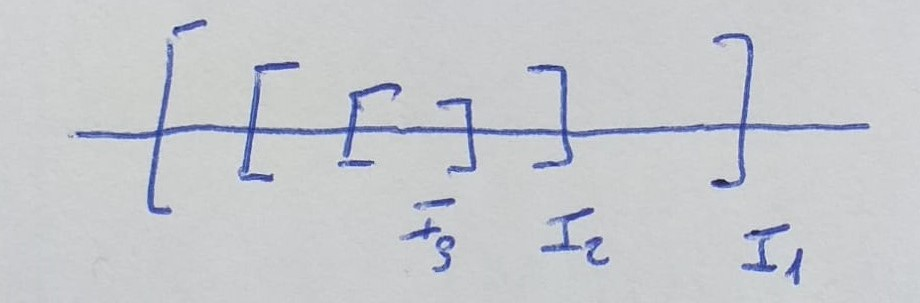
\includegraphics[scale=0.20]{Intervalos encajados}
\end{center}
También se puede expresar como:
$$\forall n\in \mathbb N : I_{n+1}\subset I_{n}$$
\end{defi}

\begin{theo}[Principio de intervalos encajados de Cantor]
Sea $F=\{I_n\}_{n\in \mathbb N}$ una familia de intervalos cerrados y encajados, entonces:
$$\bigcap_{n\in \mathbb N}I_n = [\xi, \eta] \neq \emptyset$$
donde $\xi=sup\{a_n: n\in \mathbb N\}$ y $\eta=inf\{b_n: n\in \mathbb N\}$.
\end{theo}
\begin{demo}
Llamamos $A=\{a_n: n\in \mathbb N\}$ y $B=\{b_n: n\in \mathbb N\}$, veamos que $\forall n\in \mathbb N: a_n\leq b_m$:
$$\mbox{Si }n\geq m\Rightarrow I_n\subset I_m\Leftrightarrow [a_n,b_n]\subset [a_m, b_m]\Rightarrow a_m\leq a_n\leq b_n\leq b_m$$
$$\mbox{Si }m>n\Rightarrow I_m\subset I_n\Rightarrow [a_m,b_m]\subset[a_n,b_n]\Rightarrow a_n\leq a_m\leq b_m\leq b_n$$
Lo que demuestra que cualesquiera que sean los intervalos elegidos, el extremos izquierdo de uno de ellos siempre es menor que el extremos derecho del del otro.\par 
Esto quiere decir que: $\forall n\in \mathbb N: b_m$ es cota superior del conjunto A, por lo que $\exists \xi\in \mathbb R: \xi=sup (A)$, y además $\xi\leq b_m :\forall m\in \mathbb N$, pero esto mismo afirma que $\xi$ es cota inferior de B, en consecuencia: $\exists \eta\in \mathbb R: \eta=inf(B)$ y además, $\xi\leq\eta$.\par
Veamos que: $\bigcap_{n\in \mathbb N}I_n=[\xi, \eta]\neq \emptyset$:
\begin{itemize}
\item ``$\subset$'':
$$x\in \bigcap_{n\in \mathbb N}I_n\Leftrightarrow a_n\leq x\leq b_n: \forall n \in \mathbb N\Rightarrow\begin{cases} x \mbox{ es cota superior de A}\Rightarrow x\geq\xi \\
x\mbox{ es cota inferior de B}\Rightarrow x\leq \eta\end{cases}\Rightarrow x\in [\xi,\eta]$$

\item ``$\supset$'':
$$x\in [\xi,\eta]\Leftrightarrow a_n\leq \xi\leq x\leq \eta\leq b_n: \forall n \in \mathbb N\Rightarrow a_n\leq x\leq b_n\Rightarrow x\in [a_n,b_n]=I_n: \forall n\in \mathbb N\Rightarrow x\in \bigcap_{n\in \mathbb N}I_n$$
\end{itemize}
\end{demo}

\begin{obs}
Del teorema anterior deducimos que $\xi\leq \eta$.
\end{obs}

\begin{coro}
Sea $F=\{I_n\}_{n\in \mathbb N}$ una familia de intervalos cerrados y encajados, entonces\footnote{Si $I=[a,b]$, entonces su longitud es $l(I)=b-a$}:
$$\bigcap_{n\in \mathbb N}I_n\mbox{ es un único número}\Leftrightarrow \forall \varepsilon>0: \exists n\in \mathbb N: l(I_n)<\varepsilon$$
\end{coro}
\begin{demo}
Por el teorema demostrado: $\bigcap_{n\in \mathbb N}I_n=[\xi,\eta]$, por lo que es un único número $\Leftrightarrow \xi=\eta$:

\begin{itemize}
\item ``$\Rightarrow$'':
$$\mbox{Sea }\varepsilon>0\wedge \xi=sup(A)\stackrel{Prop. Sup}{\Rightarrow} \xi-\frac{\varepsilon}{2}<a_n\leq \xi$$
Pero como además, $\xi=\eta=inf(B)$:
$$\exists m \in \mathbb N: \xi\leq b_m< \xi+ \frac{\varepsilon}{2}$$

\begin{center}
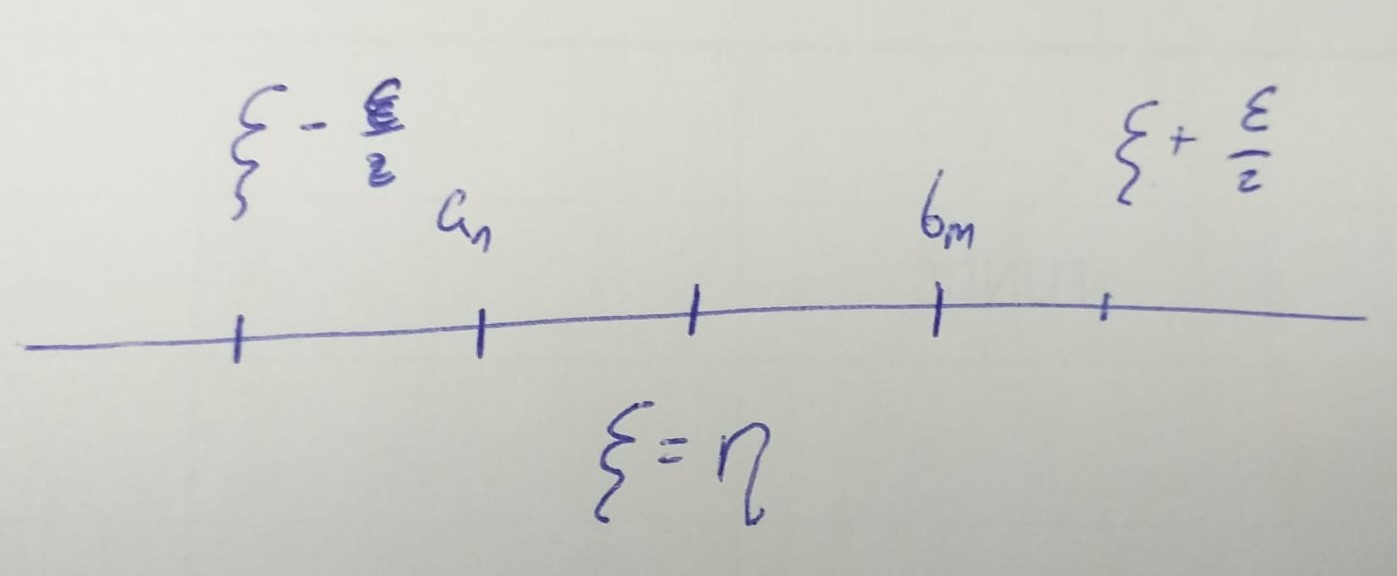
\includegraphics[scale=0.25]{corolario cantor}
\end{center}

	\begin{itemize}
	\item Ahora, si $n\geq m\Rightarrow I_n\subset I_m\Leftrightarrow a_m\leq a_n\leq b_n\leq b_m$, entonces:
$$l(I_n)=b_n-a_n\leq b_m-a_n\leq \xi+ \frac{\varepsilon}{2}-a_n<\xi+ \frac{\varepsilon}{2}-\xi+ \frac{\varepsilon}{2}=\varepsilon$$

	\item Por último, si $n<m\Rightarrow I_m\subset I_n\Leftrightarrow a_n\leq a_m\leq b_m\leq b_n$, entonces:
$$l(I_m)=b_m-a_m< \xi+\frac{\varepsilon}{2}-a_m\leq \xi+\frac{\varepsilon}{2}-a_n<\xi+\frac{\varepsilon}{2}-\xi+\frac{\varepsilon}{2}=\varepsilon$$
	\end{itemize}

\item ``$\Leftarrow$'': supongamos que $\xi<\eta$

\begin{center}
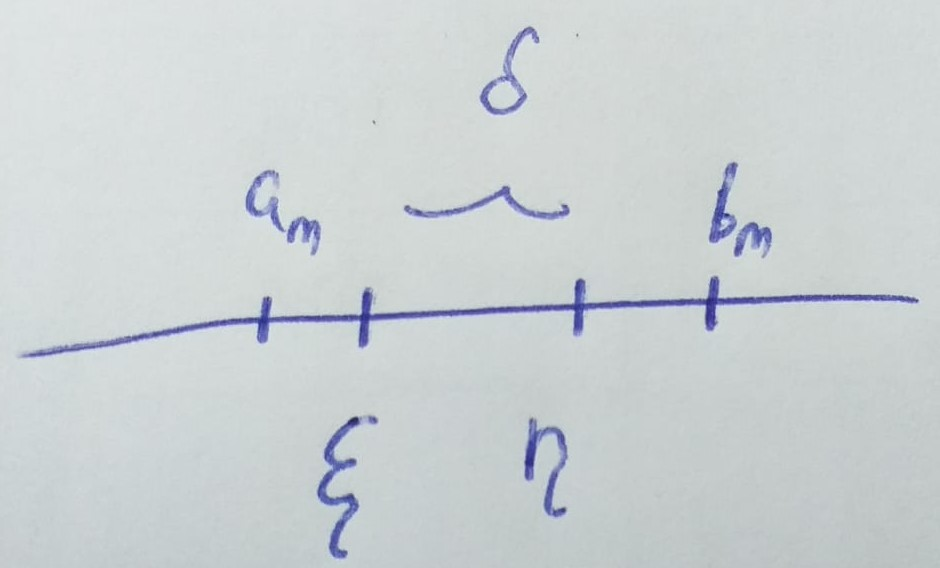
\includegraphics[scale=0.25]{corolario cantor 2}
\end{center}

$$\xi<\eta\Rightarrow \forall n \in \mathbb N: a_n\leq \xi<\eta\leq b_n\Rightarrow l(I_n)=b_n-a_n\geq \eta-a_n\geq \eta-\xi=\delta>0\Rightarrow \mbox{ \#}$$
Por que entonces decimos que los intervalos no son de la longitud que queramos porque tiene que ser mayores que un valor $\delta$ determinado.

\end{itemize}
\end{demo}

\begin{obs}
\begin{itemize}
\item Si los intervalos no son cerrados, es mentira el teorema.\par
Sea $I_n=\left(0,\frac{1}{n}\right) n\in \mathbb N$, entonces $I_{n+1}\subset I_n$ porque:
$$x\in I_{n+1}\Leftrightarrow 0<x<\frac{1}{n+1}<\frac{1}{n}\Rightarrow x\in \left(0,\frac{1}{n}\right)=I_n$$
Vemos que la intersección es vacía:
$$x\in \bigcap_{n\in \mathbb N}I_n\Leftrightarrow \forall n \in \mathbb N: 0<x<\frac{1}{n}\Rightarrow \#$$
Porque $n<\frac{1}{x}$ es absurdo porque los naturales no tienen cota superior.
\end{itemize}
\end{obs}

\subsection{Definición de la exponencial real}
Se va a prescindir de las demostraciones de las operaciones con potencias y de los resultados para raíces porque se considera que son triviales y además se prescindirá de la demostración de los enunciados posteriormente descritos por la dificultad que revisten, pero se incluyen en estos apuntes por la importancia que tienen para resultados posteriores.

Para poder definir lo que significa tener un número elevado a otro número real se atiende a la siguiente definición: sea $a,x\in \mathbb R$ y $r\in \mathbb Q$:
$$x=\sup\{r\in \mathbb Q: r<x\}=\inf\{r\in \mathbb Q: r>x\}$$

Esto implica que entendamos la exponencial real como:
$$a^x=\sup\{a^r: r<x\}=\inf\{a^r: r>x\}$$

\chapter{Sucesiones y Series}
En este capítulo vamos a estudiar las propiedades fundamentales de dos elementos matemáticos básicos para poder desarrollar todo el estudio posterior de funciones de variable real: las sucesiones y las series. Veremos unas cuantas propiedades y definiciones que luego se podrán hacer extensibles al caso continuo y aprenderemos cómo trabajar con estas funciones discretizadas.

\section{Sucesiones}
El primero de estos objetos matemáticos a estudiar son las sucesiones. Una sucesión de elementos de un conjunto es una lista infinita y numerada de elementos del mismo. Este tipo de estructura se usa para estudiar desde el crecimiento de ciertas poblaciones como para las propiedades intrínsecas a algunas funciones concretas.

\begin{defi}[Sucesión]
Sea $M$ un conjunto no vacío, una \textbf{sucesión de elementos de $M$}, que denotamos por $\{x_n\}_{n=1}^\infty\subset M$, se define como una función:
\begin{eqnarray*}
f: \mathbb N &\rightarrow& M \\
n &\longmapsto& x_n
\end{eqnarray*}
Si $M=\mathbb R$ entonces decimos que se trata de una \textbf{sucesión numérica}. 
\end{defi}

\begin{obs}
Como se trata de una lista numerada de elementos, es razonable utilizar la notación que se ha dado anteriormente, pues:
$$\{f(1),f(2),f(3), ...\}\Leftrightarrow \{x_1,x_2,x_3,...\}=\{x_n\}_{n\in \mathbb N}=\{x_n\}_{n=1}^{\infty}$$
\end{obs}

\begin{prop}[Operaciones con sucesiones numéricas]
Sean $\{x_n\}_{n=1}^{\infty}\subset \mathbb R$ y $\{y_n\}_{n=1}^{\infty}\subset \mathbb R$ dos sucesiones numéricas, entonces definimos:
\begin{itemize}
\item \textbf{Suma}: $\{x_n\}_{n=1}^{\infty}+\{y_n\}_{n=1}^{\infty}=\{x_n+y_n\}_{n=1}^{\infty}$

\item \textbf{Producto por un escalar}: Sea $a\in \mathbb R: a\cdot \{x_n\}_{n=1}^{\infty}=\{a\cdot x_n\}_{n=1}^{\infty}$

\item \textbf{Producto de sucesiones}: $\{x_n\}_{n=1}^{\infty}\cdot \{y_n\}_{n=1}^{\infty}=\{x_n\cdot y_n\}_{n=1}^{\infty}$

\item \textbf{Cociente de sucesiones}: $\frac{\{x_n\}_{n=1}^{\infty}}{\{y_n\}_{n=1}^{\infty}}=\left\lbrace\frac{x_n}{y_n}\right\rbrace_{n=1}^{\infty}$
\end{itemize}

Como las operaciones entre sucesiones se reducen a operaciones entre sus elementos, éstas heredan las propiedades de los números reales (asociativa, distributiva, ...). Por tanto, podemos observar que esta definición confiere a las sucesiones numéricas de estructura de \textbf{espacio vectorial}.
\end{prop}

\subsection{Convergencia}
Si tomamos la sucesión $\{\frac{1}{n}\}_{n=1}^{\infty}$ podemos ver que conforme los valores de $n$ aumentan, es decir, conforme avanzamos en la sucesión los elementos de la misma cada vez son más próximos a 0.
$$\frac{1}{1}, \frac{1}{2}, \frac{1}{3}, \frac{1}{4}, \cdots$$
A esta noción de acercarse cada vez más a un valor es a lo que conocemos como convergencia. Sin embargo, ha de darse una definición formal de la misma, pues podría ocurrir que nos acerquemos sólo para algunos índices concretos o que nos acerquemos a distintos valores cada vez, etc. ¿Ésta última sucesión converge?
$$\frac{1}{1}, 1, \frac{1}{2}, 1, \frac{1}{3}, 1, \frac{1}{4}, \cdots$$

\begin{defi}[Convergencia]
Sea $\{x_n\}_{n=1}^{\infty}\subset \mathbb R$ una sucesión numérica, decimos que ésta\textbf{converge o tienen límite en $l\in \mathbb R$} si y sólo si:
$$\forall \varepsilon>0: \exists n_0\in \mathbb N : \forall n\geq n_0: x_n\in (l-\varepsilon, l+\varepsilon)= E(l,\varepsilon)=|x_n-l|<\varepsilon$$
Se denota como $x_n \xrightarrow{n\rightarrow \infty}l$ o como $\lim_{n\rightarrow\infty}x_n = l$.
\end{defi}

\begin{obs}
Esto es, que fijado un $\varepsilon$ concreto, puedo encontrar un índice $n_0$ a partir del cual todos los demas $n\geq n_0$ verifican su $x_n$ correspondiente está a distancia menor que $\varepsilon$.
\end{obs}
 
\begin{prop}[Unicidad del límite]
Sea $\{x_n\}_{n=1}^\infty$ una sucesión convergente, entonces el límite de convergencia es único.
\end{prop}
\begin{demo}
Supongamos que existen dos:
$$\exists l_1,l_2: \lim_{n\rightarrow \infty}x_n=l_i$$
Como son dos números reales $l_1<l_2$, tomamos $\varepsilon=\frac{l_2-l_1}{2}$, con esto sabemos que $\exists n_0\in \mathbb N: \forall n>n_0: |x_n-l_1|<\varepsilon$ y también $\exists m_0\in \mathbb N: \forall n>m_0: |x_n-l_2|<\varepsilon\Rightarrow n\geq max\{n_0,m_0\}\Rightarrow x_n\in E(l_1,\varepsilon)=(l_1-\varepsilon, l_2+\varepsilon)\wedge x_n\in E(l_2, \varepsilon)=(l_2-\varepsilon, l_2+\varepsilon)$, estos conjuntos deben ser disjuntos pensando en el dibujo mental, así se ve que: $l_1+\varepsilon\leq l_2-\varepsilon$ concretamente $=$ porque $2\varepsilon=l_2-l_1\Rightarrow \#$
\end{demo}

\begin{prop}[Acotamiento por convergencia]
Sea $\{x_n\}_{n=1}^{\infty}\subset \mathbb R$ una sucesión convergente, entonces $\exists M>0: \forall n\in \mathbb N: |x_n|\leq M$, es decir, está acotada.
\end{prop}
\begin{demo}
Sabemos que $l$ es el límite de la sucesión así que sabemos que $\forall \varepsilon>0: \exists n_0: \forall n\geq n_0: |x_n-l|<\varepsilon$. Tomamos $\varepsilon=1$
$$\Rightarrow \exists n_0: \forall n\geq n_0: |x_n-l|<1\Rightarrow |x_n|-|l|\leq |x_n-l|<1\Rightarrow |x_n|\leq 1+l: \forall n\geq n_0$$
Demostrado los valores de $n\geq n_0$, tenemos que demostrar que se cumple para $n=1,2,3,...,n_0-1$, que como es un conjunto finito podemos decir que uno de ellos es el mayor de todos y en consecuencia $\exists \tilde{M}>0: |x_n|\leq \tilde{M}: \forall n=1,2,..., n_0-1$.\par
De este modo, nuestro número $M=max\{\tilde{M}, 1+l\}$
\end{demo}

\begin{obs}
La afirmación recíproca $\Leftarrow$ no es cierta. Teniendo la sucesión $\{x_n=(-1)^n\}_{n=1}^\infty$, supongamos que existe un $l$ que cumple la definición:
$$\exists l \in \mathbb R: \forall \varepsilon>0: \exists n_0\in \mathbb N: \forall n\geq n_0: |x_n-l|<\varepsilon$$
Si $n$ es par, $|1-l|<\varepsilon$; si $n$ es impar, $|-1-l|<\varepsilon$. Tomamos $\varepsilon=\frac{1}{2}$, entonces $|1-l|<\frac{1}{2} \wedge |-1-l|<\frac{1}{2}\Rightarrow x\in (\frac{1}{2}, \frac{3}{2})\cap (\frac{-3}{2}, \frac{-1}{2})=\emptyset$
\end{obs}

\begin{prop}[Operaciones con sucesiones convergentes]
Sean $\{x_n\}_{n=1}^\infty$ y $\{y_n\}_{n=1}^\infty \subset \mathbb R$ sucesiones convergentes a $x$ e $y$ respectivamente, entonces:
\begin{enumerate}
\item $\{x_n\}_{n=1}^\infty+\{y_n\}_{n=1}^\infty$ converge a $x+y$
$$\lim_{n\rightarrow \infty}(x_n+y_n)=\lim_{n\rightarrow \infty} x_n + \lim_{n\rightarrow \infty} y_n = x+y$$

\item Si $a\in \mathbb R$, entonces $a\cdot \{x_n\}_{n=1}^\infty$ converge a $a\cdot x$
$$\lim_{n\rightarrow \infty} a\cdot x_n=a\cdot \lim_{n\rightarrow \infty} x_n=a \cdot x$$

\item $\{x_n\}_{n=1}^\infty\cdot \{y_n\}_{n=1}^\infty$ converge a $x\cdot y$
$$\lim_{n\rightarrow \infty} x_n y_n= \lim_{n\rightarrow \infty} x_n \cdot \lim_{n\rightarrow \infty} y_n= x\cdot y$$

\item Si $x\neq 0\Rightarrow \exists n_0: \forall n\geq 0: x_n\neq 0$ y entonces $\frac{\{y_n\}_{n=1}^\infty}{\{x_n\}_{n=1}^\infty}$ converge a $\frac{y}{x}$
$$\lim_{n\rightarrow \infty}\frac{y_n}{x_n}=\frac{\lim_{n\rightarrow \infty} y_n}{\lim_{n\rightarrow \infty} x_n}=\frac{y}{x}$$

\item $\{|x_n|\}_{n=1}^\infty$ converge a $|x|$
$$\lim_{n\rightarrow \infty} |x_n|=\left|\lim_{n\rightarrow \infty} x_n\right|=|x|$$
\end{enumerate}
\end{prop}
\begin{demo}
\begin{enumerate}
\item Queremos ver que para $\forall \varepsilon>0: |(x_n+y_n)-(x+y)|<\varepsilon$:

$$|(x_n+y_n)-(x+y)|=|x_n-x+y_n-y|\leq |x_n-x|+|y_n-y|$$
Para ello sabemos que como $\varepsilon>0\Rightarrow\exists n_0^1: \forall n\geq n_0^1: |x_n-x|<\frac{\varepsilon}{2}$ y que $\exists n_0^2: \forall n \geq n_0^2: |y_n-y|<\frac{\varepsilon}{2}$, pero hay que garantizar que esto ocurra eligiendo el elemento correcto:
$$n_0=max\{n_0^1, n_0^2\}\Rightarrow \forall n\geq n_0\wedge n\geq m_0\Rightarrow |x_n-x|+|y_n-y|<\varepsilon$$
Porque $|x_n-x|<\frac{\varepsilon}{2}$ y $|y_n-y|<\frac{\varepsilon}{2}\Rightarrow |x_n-x|+|y_n-y|<\varepsilon$.
\vspace{0.35cm}

\item Suponiendo\footnote{$a=0\Rightarrow 0\cdot \{x_n\}_{n=1}^\infty=\{0\}_{n=1}^\infty=0$} $a\neq 0$ y sea $\varepsilon>0$ queremos probar que $|ax_n-ax|<\varepsilon$:

$$|a\cdot x_n-a\cdot x|=|a\cdot (x_n-x)|=|a|\cdot |x_n-x|$$
$$\Rightarrow |a|\cdot |x_n-x| < |a|\cdot \frac{\varepsilon}{|a|}=\varepsilon$$
Pero como sabemos que sea $\varepsilon>0\Rightarrow \exists n_0\in \mathbb N: \forall n\geq n_0: |x_n-x|<\frac{\varepsilon}{|a|}$, entonces:
$$|a|\cdot |x_n-x| < |a|\cdot \frac{\varepsilon}{|a|}=\varepsilon$$

\item Sea $\varepsilon>0$, queremos probar que $|x_ny_n-xy|<\varepsilon$:
$$|x_ny_n-xy|=|x_ny_n-xy+x_ny-x_ny|=|x_n(y_n-y)+y(x_n-x)|\leq |x_n||y_n-y|+|y||x_n-x|$$

Por la proposición anterior como $x_n$ es convergente, es acotada así que $\exists M>0: |x_n|\leq M: \forall n\in \mathbb N$, por lo que:
$$|x_n||y_n-y|+|y||x_n-x|< M|y_n-y|+|y||x_n-x|$$

De este modo como si $y=0$, entonces:
$$\varepsilon>0\Rightarrow\exists n_0: \forall n\geq n_0: |y_n-y|<\frac{\varepsilon}{M}\Rightarrow M|y_n-y|+|y||x_n-x|=M|y_n-y|<M\cdot \frac{\varepsilon}{M}=\varepsilon$$

Si $y\neq 0$, entonces:\par
$\varepsilon>0\Rightarrow\exists n_0^1: \forall n\geq n_0^1: |x_n-x|<\frac{\varepsilon}{2|y|}$ y que $\exists n_0^2: \forall n \geq n_0^2: |y_n-y|<\frac{\varepsilon}{2M}\Rightarrow n_0=max\{n_0^1, n_0^2\}\Rightarrow \forall n\geq n_0:$
$$M|y_n-y|+|y||x_n-x|< M\frac{\varepsilon}{2M}+|y|\frac{\varepsilon}{2|y|}=\varepsilon$$

\item Como hemos probado el producto, basta probar que $\lim_{n\rightarrow \infty} \frac{1}{x_n}=\frac{1}{x}$.\par
Como $x\neq 0$:

\begin{center}
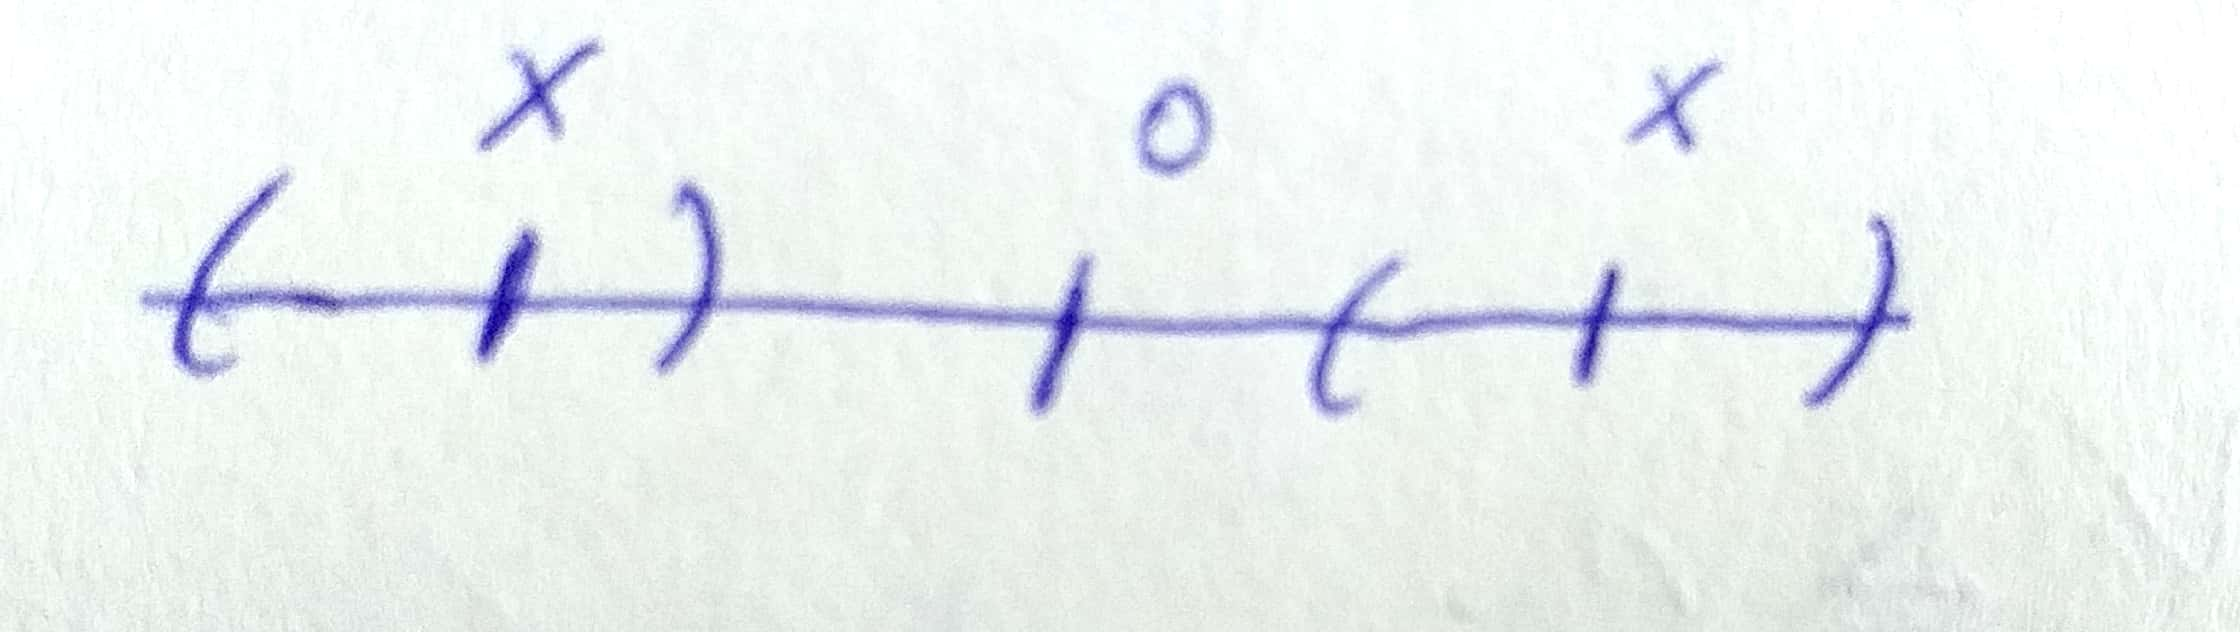
\includegraphics[scale=0.05]{x a cero}
\end{center}

$$\forall \varepsilon>0: \exists n_0\in \mathbb N: \forall n\geq n_0: |x_n-x|<\varepsilon$$
$$\mbox{Sea }\varepsilon=\frac{|x|}{2}\Rightarrow \exists n_0: \forall n\geq n_0: |x_n-x|<\frac{|x|}{2}$$
$$\mbox{ Vemos que } |x|-|x_n|\leq |x_n-x|<\frac{|x|}{2}\Rightarrow |x|-\frac{|x|}{2}\leq |x_n|: \forall n\geq n_0\Leftrightarrow 0< \frac{|x|}{2}\leq |x_n|$$
Con esto queda probado que a partir de un cierto índice, los $|x_n|$ son distintos de 0, por lo que puedo decir que $\lim_{n\rightarrow \infty} \frac{1}{x_n}=\frac{1}{x}$ es correcto.\par

Veamos ahora que $x_n\neq 0, \forall n\geq n_0: \lim_{n\rightarrow \infty}\frac{1}{x_n}=\frac{1}{x}$:
$$\mbox{Sea }\varepsilon>0\Rightarrow |\frac{1}{x_n}-\frac{1}{x}|=|\frac{x-x_n}{x\cdot x_n}|=\frac{|x-x_n|}{|x||x_n|}$$

Antes habíamos probado que $0< \frac{|x|}{2}\leq |x_n|\Rightarrow \frac{1}{|x_n|}\leq \frac{2}{|x|}$. Con lo cual para $n\geq n_0$:
$$\frac{|x-x_n|}{|x||x_n|}\leq \frac{2|x-x_n|}{|x|^2}$$

Ahora si $\varepsilon>0\Rightarrow \exists N_0\in \mathbb N: \forall n\geq N_0: |x_n-x|< \frac{|x|^2}{2}\cdot \varepsilon$, con lo cual si tomamos como $n_0^1=\{n_0,N_0\}$ se dan las dos condiciones por lo que:
	$$n\geq n_0^1\Rightarrow \frac{2|x-x_n|}{|x|^2}< \frac{2}{|x|^2}\cdot \frac{|x|^2}{2}\cdot \varepsilon=\varepsilon$$

\vspace{0.40cm}

\item Sea $\varepsilon>0$ queremos medir $||x_n|-|x||$, pero sabemos que:
$$||x_n|-|x||\leq |x_n-x|<\varepsilon$$
Esto último porque sabemos que dado $\varepsilon>0 : \exists n_0\in \mathbb N: \forall n\geq n_0$
\end{enumerate}
\end{demo}

\begin{prop}[Convergencia y Orden]
Sean $\{x_n\}_{n=1}^\infty$ y $\{y_n\}_{n=1}^\infty\subset \mathbb R$ sucesiones convergentes a $x,y\in \mathbb R$ respectivamente, entonces:
\begin{enumerate}
\item Si $\exists n_0 \in \mathbb{N}: \forall n\in \mathbb{N}: x_n\geq 0 \Rightarrow x\geq 0$
\item Si $\exists n_0 \in \mathbb{N}: \forall n\in \mathbb{N}: x_n\leq y_n \Rightarrow x\leq y$
\item Si $\exists a,b\in \mathbb R$: y $\exists n_0 \in \mathbb{N}: \forall n\in \mathbb{N}: a\leq x_n\leq b\Rightarrow a\leq x\leq b: \forall n \in \mathbb N$
\item \textbf{Regla del sandwich}: Si $\exists n_0 \in \mathbb{N}: \forall n\in \mathbb{N} : x_n\leq y_n$ y $x=y$, entonces cualquier sucesión $\{z_n\}_{n=1}^\infty $ que verifique $\exists n_0 \in \mathbb{N}: \forall n\in \mathbb{N} : x_n\leq z_n\leq y_n$ es convergente a $x(=y)$.
\end{enumerate}
\end{prop}
\begin{demo}
\begin{enumerate}
\item Si $x<0$, entonces $\forall \varepsilon >0: \exists n_0\in \mathbb N: \forall n\geq n_0: |x_n-x|<\varepsilon$, cogemos por tanto un epsilon tal que el extremo derecho sea negativo: $x+\varepsilon<0$, con lo cual $\exists n_0\in \mathbb N: \forall n \geq n_0: x_n\in (x-\varepsilon,x+\varepsilon)\Rightarrow x_n<x+\varepsilon<0\Rightarrow \#$

\begin{center}
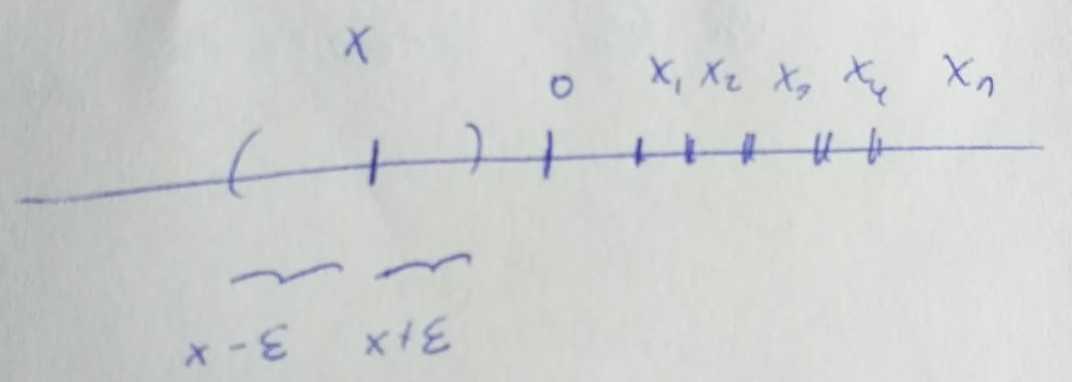
\includegraphics[scale=0.25]{limite negativo}
\end{center}

\item Sea $z_n=y_n-x_n\geq 0: \forall n\in \mathbb N$ por lo que $z_n$ converge a $y-x\Rightarrow y-x\geq 0\Leftrightarrow y\geq x$

\item Sea $z_n=x_n-a\geq 0: \forall n \in \mathbb N$, esta converge a $x-a\stackrel{1.}{\geq}0$ y sea $w_n=b-x_n$, esta converge a $b-x\geq 0$, en consecuencia: $b\geq x\geq a\Rightarrow x\in [a,b]$

\item Definimos como $w_n=y_n-x_n\geq 0: \forall n \in \mathbb N$, como converge a $y-x\Rightarrow y-y=0$, luego el límite es 0. Ahora medimos la distancia entre $z_n$ y $x_n$:
$$0\leq z_n-x_n\leq y_n-x_n\Rightarrow \{z_n-x_n\}_{n=1}^\infty\stackrel{\infty}{\rightarrow} 0: \forall \varepsilon>0$$
Esto puede hacerse porque estaba verificado que $w_n$ tendía a cero: dado $\varepsilon>0: \exists n_0\in \mathbb N: \forall n\geq n_0: w_n<\varepsilon\Rightarrow z_n-x_n<\varepsilon$. Con lo cual si tomamos:
$$z_n=(z_n-x_n)+x_n\Rightarrow \lim_{n\rightarrow \infty} z_n=\lim_{n\rightarrow \infty} (z_n-x_n)+ \lim_{n\rightarrow \infty} x_n=0+x=x$$
\end{enumerate}
\end{demo}

\subsubsection{Divergencia}
En ocasiones, una sucesión no converge a un valor concreto sino que se acerca con uniformidad a valores cada vez más grandes o más pequeños, es decir, a $\pm\infty$. Precisamente esta idea es la noción de convergencia y para poder trabajar con ella es necesario redefinir las operaciones con límites y qué significa eso de tender a infinito.

\begin{defi}[Monotonía]
Una sucesión de números de reales $\{x_n\}_{n=1}^\infty\subset \mathbb R$, se llama \textbf{monótona creciente\footnote{Decimos que es estrictamente creciente si la desigualdad es estricta}} si:
$$\forall n\in \mathbb N: x_n\leq x_{n+1}\Rightarrow \{x_n\}_{n=1}^\infty \uparrow$$
Una sucesión de números reales $\{x_n\}_{n=1}^\infty\subset \mathbb R$, se llama \textbf{monótona decreciente\footnote{Decimos que es estrictamente decreciente si la desigualdad es estricta}} si:
$$\forall n\in \mathbb N: x_{n+1}\leq x_n \Rightarrow \{x_n\}_{n=1}^\infty \downarrow$$
\end{defi}

\begin{prop}
Sea $\{x_n\}_{n=1}^\infty$ una sucesión monótona creciente y acotada superiormente, entonces es convergente al \textbf{supremo} de los elementos de la sucesión.
$$\{x_n\}_{n=1}^\infty \uparrow \wedge \mbox{ es acotada superiormente}\Rightarrow \lim_{n\rightarrow \infty} \{x_n\}=l=\sup\{x_n: \forall n\in \mathbb N\}$$
Sea $\{x_n\}_{n=1}^\infty$ una sucesión monótona decreciente y acotada inferiormente, entonces es convergente al \textbf{ínfimo} de los elementos de la sucesión.
$$\{x_n\}_{n=1}^\infty \uparrow \wedge \mbox{ es acotada inferiormente}\Rightarrow \lim_{n\rightarrow \infty} \{x_n\}=l=\inf\{x_n: \forall n\in \mathbb N\}$$
\end{prop}
\begin{demo}
\begin{enumerate}
\item 
$$\mbox{Acotada superiormente}\Rightarrow \exists M\in \mathbb R: x_n\leq M: \forall n\in \mathbb N\Rightarrow \exists l=\sup\{x_n: n\in \mathbb N\}$$
Por ser supremo, si $\varepsilon>0$, entonces $\exists n_0\in N: l-\varepsilon<x_{n_0}\leq l$, así que:
$$\forall n\geq n_0\Rightarrow l-\varepsilon< x_{n_0}\leq x_n\leq l \Rightarrow x_n\in (l-\varepsilon, l+\varepsilon)$$
No hay contradicción por que aunque nunca se encuentren más allá de $l$, lo escrito no es mentira y en consecuencia cumplen las premisas de convergencia.

\item 
$$\mbox{Por ser acotada inferiormente}\Rightarrow \exists m\in \mathbb R: m\leq x_n: \forall n\in \mathbb N\Rightarrow \exists l=\inf\{x_n: \forall n\in \mathbb N\}$$
Por ser ínfimo, si $\varepsilon>0$, entonces $\exists n_0\in N: l\leq x_{n_0}<l+\varepsilon$, así que:
$$\forall n\geq n_0\Rightarrow l< x_n\leq x_{n_0} <l+\varepsilon \Rightarrow x_n\in (l-\varepsilon, l+\varepsilon)$$
Del mismo modo que antes, se cumplen las premisas de convergencia sin mentir en ningún punto.
\end{enumerate}
\end{demo}

\begin{defi}[Divergencia]
Sea $\{x_n\}_{n=1}^\infty\subset \mathbb R$ una sucesión numérica decimos que ésta \textbf{diverge o tiende a $\infty$}\footnote{Del mismo modo, la definición para la divergencia a menos infinito viene dada por $\forall M>0: \exists n_0\in \mathbb N: \forall n \geq n_0: x_n\leq -M$} si y sólo si:
$$\lim_{n\rightarrow \infty} x_n=-\infty \Leftrightarrow \forall M>0: \exists n_0\in \mathbb N: \forall n \geq n_0: x_n\geq M$$
Es decir, que diverge si para cualquier constante que escojamos hay un término a partir del cual todos los demás son más grandes que dicha constante.
\end{defi}

\begin{prop}[Divergencia y Monotonía]
Sea $\{x_n\}_{n=1}^\infty\subset \mathbb R$ una sucesión numérica, entonces
\begin{enumerate}
\item $\{x_n\}_{n=1}^\infty \uparrow$ y no acotada superiormente $\Rightarrow \lim_{n\rightarrow \infty} x_n=\infty$

\item $\{x_n\}_{n=1}^\infty \downarrow$ y no acotada inferiormente $\Rightarrow \lim_{n\rightarrow \infty} x_n=-\infty$
\end{enumerate}
\end{prop}
\begin{demo}
\begin{enumerate}
\item Sea $M>0$ como $\{x_n\}_{n=1}^\infty $ no es acotada superiormente, entonces $\exists n_0\in \mathbb N: M\leq x_{n_0}$. Si $n\geq n_0\Rightarrow M\leq x_{n_0}\leq x_n$

\item Sea $M>0$ como $\{x_n\}_{n=1}^\infty $ no es acotada inferiormente, entonces $\exists n_0\in \mathbb N: -M\geq x_{n_0}$. Si $n\geq n_0\Rightarrow -M\geq x_{n_0}\geq x_n$
\end{enumerate}
\end{demo}

\begin{obs}
Cabe destacar que gracias a esta proposición vemos que si la sucesión diverge, entonces no es acotada.
\end{obs}

\begin{prop}
Sea $\{x_n\}_{n=1}^\infty \subset \mathbb R$ una sucesión numérica, entonces:
\begin{enumerate}
\item Si $\lim_{n\rightarrow \infty} x_n=\pm \infty$, entonces $\lim_{n\rightarrow \infty} \frac{1}{x_n}=0$

\item Si $x_n>0: \forall n\in \mathbb N$ y $\lim_{n\rightarrow \infty} x_n=0$, entonces $\lim_{n\rightarrow \infty} \frac{1}{x_n}=\infty$

\item Si $x_n<0: \forall n\in \mathbb N$ y $\lim_{n\rightarrow \infty}x_n=0$, entonces $\lim_{n\rightarrow \infty} \frac{1}{x_n}=-\infty$
\end{enumerate}
\end{prop}
\begin{demo}
\begin{enumerate}
\item Supongamos que $\lim_{n\rightarrow \infty} x_n=\infty$ y sea $\varepsilon>0$, tenemos que probar que $|\frac{1}{x_n}-0|<\varepsilon$:
$$\mbox{Sea M}=\frac{1}{\varepsilon}\Rightarrow \exists n_0\in \mathbb N: \forall n\geq n_0: x_n> \frac{1}{\varepsilon}=M\Rightarrow \frac{1}{x_n}<\varepsilon\Leftrightarrow |\frac{1}{x_n}|<\varepsilon$$

Supongamos que $\lim_{n\rightarrow \infty} x_n=-\infty$ y sea $\varepsilon>0$, tenemos que probar que $|\frac{1}{x_n}-0|<\varepsilon$:
$$\mbox{Sea M}=\frac{1}{\varepsilon}\Rightarrow \exists n_0\in \mathbb N: \forall n\geq n_0: x_n< \frac{-1}{\varepsilon}=-M\Rightarrow \frac{-1}{x_n}<\varepsilon\Leftrightarrow |\frac{1}{x_n}|<\varepsilon$$

\item Sea $M>0$ queremos probar que $\frac{1}{x_n}>M$ de un índice en adelante:
$$\mbox{Sea }M>0,\mbox{ tomamos } \varepsilon=\frac{1}{M}\Rightarrow \exists n_0\in \mathbb N: \forall n\geq n_0: |x_n-0|<\varepsilon\Leftrightarrow |x_n|=x_n<\varepsilon=\frac{1}{M}\Rightarrow M<\frac{1}{x_n}$$

\item Sea $M>0$, queremos probar que $\frac{1}{x_n}<-M$ de un índice en adelante:
$$\mbox{Sea }M>0,\mbox{ tomamos }\varepsilon=\frac{1}{M}>0\Rightarrow \exists n_0\in \mathbb N: \forall n\geq n_0: |x_n-0|<\varepsilon\Leftrightarrow |x_n|=-x_n<\varepsilon=\frac{1}{M}\Rightarrow \frac{1}{x_n}<-M$$
\end{enumerate}
\end{demo}

\begin{defi}[$\mathbb{R}$ ampliado]
Denotamos por ``$\mathbb R$ ampliado'' al conjunto
$$\overline{\mathbb R}=\mathbb R\cup \{\infty\}\cup \{-\infty\}$$
Además, entendemos las siguientes operaciones en dicho conjunto:
\begin{enumerate}
\item Si $x=\infty$, entonces $x+y=\infty$ si $y\in \mathbb R\cup \{\infty\}$
\item $a\cdot x=\infty$ si $a\in (0,\infty)$ y $a\cdot x=-\infty $ si $a\in (-\infty, 0)$
\item $xy=\infty$ si $y\in (0,\infty)\cup\{\infty\} \mbox{ y } xy=-\infty$ si $y\in (-\infty,0)\cup\{-\infty\} $
\item $\frac{x}{y}=\infty $ si $y\in (0,\infty) \mbox{ y } \frac{x}{y}=-\infty $ si $y\in (-\infty,0) $
\item Si $x=\infty$ y $x\leq y$, entonces $y=\infty$
\end{enumerate}
\end{defi}

\begin{prop}[Operaciones con límites infinitos]
Sea $\{x_n\}_{n=1}^\infty$ y $\{y_n\}_{n=1}^\infty\subset \mathbb R$ dos sucesiones convergentes a $x,y\in \overline{\mathbb R}$ respectivamente, entonces:
\begin{enumerate}
\item $\lim_{n\rightarrow \infty}(x_n+y_n)=x+y$
\item Si $a\in \mathbb R$, entonces $\lim_{n\rightarrow \infty} (a\cdot x_n)=a\cdot x$
\item $\lim_{n\rightarrow \infty}(x_n\cdot y_n)=x\cdot y$
\item $\lim_{n\rightarrow \infty}\frac{x_n}{y_n}=\frac{x}{y}$
\item Si $x_n\leq y_n \Rightarrow x\leq y$
\end{enumerate}
\end{prop}

\begin{obs}
Vemos que quedan excluidas las situaciones $\infty -\infty$, $0\cdot \infty$, $\frac{\infty}{\infty}$, $\frac{\infty}{0}$, que son conocidas como \textbf{indeterminaciones}.
\end{obs}

\begin{theo}[Criterio del Cociente y la Raíz]
Sea $\{x_n\}_{n=1}^\infty$ una sucesión numérica, entonces:
\begin{align*}
\lim_{n\rightarrow \infty}\left|\frac{x_{n+1}}{x_n}\right|<1 &\Rightarrow \lim_{n\rightarrow \infty} x_n=0 \\
\lim_{n\rightarrow \infty}\left|\frac{x_{n+1}}{x_n}\right|>1 &\Rightarrow \lim_{n\rightarrow \infty} |x_n|=\infty \\
\lim_{n\rightarrow \infty}\sqrt[n]{|x_n|}<1 &\Rightarrow \lim_{n\rightarrow \infty} x_n=0\\
\lim_{n\rightarrow \infty}\sqrt[n]{|x_n|}>1 &\Rightarrow \lim_{n\rightarrow \infty} |x_n|=\infty
\end{align*}
Cabe destacar que el caso en que dichos límites sean exactamente 1 no aporta ningún tipo de información acerca de la convergencia de la sucesión.
\end{theo}


\begin{ej}
Sea $p>0$, entonces $x_n=\frac{1}{n^p}: n\in \mathbb N$ veamos que $\lim_{n\rightarrow \infty} \frac{1}{n^p}=0$
$$1\leq n<n+1\Rightarrow n^p< (n+1)^p\Rightarrow x_{n+1}=\frac{1}{(n+1)^p}<\frac{1}{n^p}=x_n\Rightarrow \{x\}_{n=1}^\infty \downarrow$$
Desde luego se observa que el ínfimo de los elementos de la sucesión es 0, y como hemos demostrado que toda sucesión decreciente acotada inferiormente converge a su supremo, lo demostramos:
$$\mbox{Si }\exists \alpha: 0<\alpha\leq \frac{1}{n^p}: \forall n\in \mathbb N\Leftrightarrow n^p\leq \frac{1}{\alpha}\Rightarrow n\leq \left(\frac{1}{\alpha}\right)^{\frac{1}{p}}: \forall n \in \mathbb N\Rightarrow \#$$
Porque los naturales no pueden tener cota superior.
\end{ej}

\begin{ej}
Si $r\in \mathbb R$, entonces $x_n=r^n: n\in \mathbb N$
\begin{itemize}
\item Si $r=0$:
$$x_n=0\Rightarrow \lim_{n\rightarrow \infty}x_n=0$$

\item Si $r=1$:
$$x_n=1\Rightarrow \lim_{n\rightarrow \infty}x_n=1$$

\item Si $0<r<1$
$$r^{n+1}<r^n\Leftrightarrow x_{n+1}<x_n: \forall n\in \mathbb N\Rightarrow \{x_n\}_{n=1}^\infty \downarrow \stackrel{acot. inf.}\Rightarrow \exists \lim =\inf$$

Probamos que el ínfimo es 0 de nuevo:
$$\mbox{Si }\exists\alpha: 0<\alpha \leq r^n: \forall n\in \mathbb N\Rightarrow \frac{1}{\alpha}\geq\frac{1}{r^n}=\left(\frac{1}{r}\right)^n:\forall n\in \mathbb N\Rightarrow \# \mbox{ porque }\frac{1}{r}>1 \mbox{ y }\{x^n: x>1\wedge n\in \mathbb N\}\mbox{ no acot.}$$

\item Si $r>1$
$$r^{n+1}>r^n\Leftrightarrow x_{n+1}>x_n\Rightarrow \{x_n\}\uparrow \Rightarrow \{x_n\}\mbox{ no esta acotada sup.}$$

Porque si realmente lo estuviese entonces:
$$r^n\leq M: \forall n\in \mathbb N: r>1\Rightarrow \#\mbox{ por la propiedad arquimediana del producto}\Rightarrow \lim_{n\rightarrow\infty} r^n=\infty$$

\item Si $-1<r<0$:
$$0<|r|<1\Rightarrow 0\leq |r^n|=|r|^n\stackrel{\mbox{caso } 0<r<1}{\Rightarrow }\lim_{n\rightarrow \infty} |r|^n=0\stackrel{Regla Sandwich}{\Rightarrow} \lim_{n\rightarrow \infty} |r^n|=0\Rightarrow \lim_{n\rightarrow \infty} r^n=0$$

\item Si $r=-1$:
$$\mbox{No hay límite}$$

\item Si $r<-1$:

$$\begin{cases}x_{2k}=r^{2k}=(r^2)^k\stackrel{n\rightarrow \infty}{\rightarrow} \infty \\
x_{2k+1}=r^{2k+1}=r^{2k}\cdot r \stackrel{n\rightarrow \infty}{\rightarrow} -\infty\end{cases}\Rightarrow \nexists \lim$$
\end{itemize}
\end{ej}


\begin{ej}
Sea $a>0$, $x_n=\sqrt[n]{a}$, veamos que $\lim_{n\rightarrow \infty}x_n=1$:
\begin{itemize}
\item Si $a=1$
$$\sqrt[n]{1}=1:\forall n\in \mathbb N\Rightarrow \lim =1$$

\item Si $a>1$
$$\frac{1}{n+1}<\frac{1}{n}\Rightarrow a^{\frac{1}{n+1}}<a^{\frac{1}{n}}\Leftrightarrow \sqrt[n+1]{a}<\sqrt[n]{a}\Leftrightarrow x_{n+1}< x_n\Rightarrow \{x_n\}_{n=1}^\infty \downarrow$$
Ahora basta con probar que el ínfimo de dicha sucesión es el 1 y por las proposiciones citadas, estaría demostrado que es su límite.
$$\exists m: 1<m\leq \sqrt[n]{a}: \forall n\in \mathbb N\Rightarrow \alpha^n\leq a \forall n\in \mathbb N\Rightarrow \#\mbox{ por la prop. Arqui. Produc porque }\alpha>1$$

\item Si $0<a<1$
$$\frac{1}{a}>1\Rightarrow \sqrt[n]{\frac{1}{a}}=\frac{1}{\sqrt[n]{a}}\Rightarrow \lim_{n\rightarrow \infty} \frac{1}{\sqrt[n]{a}}=\frac{1}{\lim_{n\rightarrow \infty} \sqrt[n]{a}}=\frac{1}{1}=1$$
\end{itemize}
\end{ej}

\begin{ej}
Vamos a probar que $\lim_{n\rightarrow \infty}\sqrt[n]{n}=1$, viendo que
$$n\geq 1\Rightarrow \sqrt[n]{n}\geq 1\Rightarrow \sqrt[n]{n}=1+k_n: k_n>0\Rightarrow n=(1+k_n)^n=\sum_{j=0}^n \binom{n}{j}k_n^j\geq 1+\binom{n}{2}k_n^2=1+\frac{n(n+1)}{2\Rightarrow}$$
$$\Rightarrow n-1\geq \frac{n(n+1)}{2}\cdot k_n^2\Leftrightarrow 0\leq k_n^2\leq \frac{2}{n}\stackrel{ReglaSandwich}{\Rightarrow} k_n^2\stackrel{n\rightarrow \infty}{\rightarrow} 0\Rightarrow k_n\stackrel{n\rightarrow \infty}{\rightarrow} 0\Rightarrow \sqrt[n]{n}=1+k_n \stackrel{n\rightarrow \infty}{\rightarrow} 1+0=1$$

Se observa que en la desigualdad a partir del sumatorio me he quedado solo con los sumandos de $j=0$ y $j=2$ por lo que se cumple la desigualdad mostrada.
\end{ej}

\begin{theo}[Criterio de Stoltz]
Sea una $\{y_n\}_{n=1}^\infty\subset \mathbb R$ una sucesión estrictamente creciente y divergente a infinito y $\{x_n\}_{n=1}^\infty\subset \mathbb R$ otra sucesión cualquiera, entonces:
$$\lim_{n\rightarrow \infty} \frac{x_{n+1}-x_n}{y_{n+1}-y_n}=l\in \overline{\mathbb R}\Rightarrow \lim_{n\rightarrow \infty} \frac{x_n}{y_n}=l\in \overline{\mathbb R}$$
\end{theo}
\begin{demo}
Sea $m,n\in \mathbb N: m<n$, entonces escribimos:
$$x_n=x_m+(x_n-x_m)=x_m+x_n-x_{n-1}+x_{n-1}-x_m=x_m+\sum_{k=m+1}^n (x_k-x_{k-1})$$

Como $y_n\stackrel{n\rightarrow\infty}{\rightarrow} \infty$ podemos suponer que $y_n>0: \forall n$, con lo cual si dividimos entre $y_n$:
$$\frac{x_n}{y_n}=\frac{x_m}{y_n}+\frac{1}{y_n}\sum_{k=m+1}^n (x_k-x_{k-1})=\frac{x_m}{y_n}+\frac{1}{y_n}\sum_{k=m+1}^n \frac{(x_k-x_{k-1})}{y_k-y_{k-1}}\cdot (y_k-y_{k-1})$$

\begin{itemize}
\item Supongamos ahora que $l\in \mathbb R$: hacemos lo mismo $x_n=l\cdot y_n$, con lo cual queda:
$$l=\frac{l\cdot y_m}{y_n}+\frac{1}{y_n}+\sum_{k=m+1}^n (y_k-y_{k-1})\cdot l$$

Ahora vemos que:
$$\frac{x_n}{y_n}-l=\frac{x_m-l\cdot y_m}{y_n}+\frac{1}{y_n}\sum_{k=m+1}^n \left(\frac{x_k-x_{k-1}}{y_k-y_{k-1}}-l\right)\cdot (y_k-y_{k-1})$$

Y si tomamos el valor absoluto:
$$\left|\frac{x_n}{y_n}-l\right|\leq \left|\frac{x_m-l\cdot y_m}{y_n}\right|+\frac{1}{y_n}\sum_{k=m+1}^n \left|\frac{x_k-x_{k-1}}{y_k-y_{k-1}}-l\right|\cdot (y_k-y_{k-1})$$

Dado $\varepsilon>0: \exists n_0\in \mathbb N: \forall k\geq n_0$, entonces:
$$\left|\frac{x_{k+1}-x_k}{y_{k+1}-y_k}-l\right|<\varepsilon\stackrel{m=n_0}{\Rightarrow} \forall n\geq n_0: \left|\frac{x_n}{y_n}-l\right|\leq \left|\frac{x_{n_0}-ly_{n_0}}{y_n}\right|+\frac{1}{y_n}\sum_{k=n_0+1}^n (y_k-y_{k-1})\frac{\varepsilon}{2}=$$
$$\left|\frac{x_{n_0}-ly_{n_0}}{y_n}\right|+\frac{\varepsilon}{2}\left(1-\frac{y_{n_0}}{y_n}\right)\stackrel{1-\lambda<1}{\leq} \left|\frac{x_{n_0}-ly_{n_0}}{y_n}\right|+\frac{\varepsilon}{2}\stackrel{y_n\rightarrow\infty}{\Rightarrow} \exists n_1\in \mathbb N: n\geq n_1: \left|\frac{x_{n_0}-ly_{n_1}}{y_n}\right|<\frac{\varepsilon}{2}$$

Ahora este $n_1$ podemos suponerlo $n_1\geq n_0$ porque si no cogeríamos el más grande de ambos para que se verificasen ambas cosas, con lo cual:
$$\left|\frac{x_{n_0}-ly_{n_0}}{y_n}\right|+\frac{\varepsilon}{2}<\frac{\varepsilon}{2}+\frac{\varepsilon}{2}=\varepsilon $$

\item Supongamos ahora que $l=\infty$, entonces dado $M>0: \exists n_0\in \mathbb N: \forall k\geq n_0$, tenemos:
$$\left|\frac{x_{k+1}-x_{k}}{y_{k+1}-y_k}\right|>2M\stackrel{m=n_0}{\Rightarrow} \forall n\geq n_0: \frac{x_n}{y_n}\geq \frac{x_{n_0}}{y_n}+ 2M\frac{1}{y_n}\cdot \sum_{k=n_0+1}^n (y_k-y_{k-1})=\frac{x_{n_0}}{y_n}+ 2M\frac{1}{y_n}\cdot (y_n-y_{n_0})=$$
$$=2M + \frac{x_{n_0}-2My_{n_0}}{y_n}=2M + \frac{x_{n_0}}{y_n}-2M\frac{y_{n_0}}{y_n}\stackrel{y_n\rightarrow \infty}{\Rightarrow} \exists n_1\in \mathbb N: n\geq n_1: \frac{x_{n_0}}{y_n}-2M\frac{y_{n_0}}{y_n}\geq -M\Rightarrow $$
$$\Rightarrow 2M + \frac{x_{n_0}}{y_n}-2M\frac{y_{n_0}}{y_n}\geq M$$

\item Supongamos ahora que $l=-\infty$, entonces la sucesión $\{-x_n\}_{n=1}^\infty$ verifica que:
$$\frac{-x_{n+1}-(-x_n)}{y_{n+1}-y_n}=\frac{-(x_{n+1}-x_n)}{y_{n+1}-y_n} \rightarrow\infty \Rightarrow \frac{-x_n}{y_n}\rightarrow \infty\Rightarrow \frac{x_n}{y_n}\rightarrow \infty$$
\end{itemize}
\end{demo}

\begin{obs}
El recíproco es completamente falso, pues
$$\frac{x_n}{y_n}=\frac{(-1)^n}{n}\Rightarrow \lim_{n\rightarrow \infty} \frac{(-1)^n}{n}=0$$
pero vemos que:
$$\frac{x_{n+1}-x_n}{y_{n+1}-y_n}=\frac{(-2)(-1)^n}{1}\Rightarrow \nexists \lim x_n$$
\end{obs}

\begin{ej}
Sea $x_n=n$ y $y_n=2^n$, entonces:
$$\frac{x_{n+1}-x_n}{y_{n+1}-y_n}=\frac{1}{2^{n+1}-2^n}=\frac{1}{2^n}\stackrel{n\rightarrow \infty}{\rightarrow} 0\Rightarrow \lim_{n\rightarrow \infty}\frac{n}{2^n}=0$$
\end{ej}

\begin{ej}
Sea $p>0$ y $\alpha\in \mathbb R$, entonces $\lim_{n\rightarrow\infty}\frac{n^\alpha}{(1+p)^n}=0$:
\begin{itemize}
\item Caso $\alpha\leq 0$:
$$\alpha\leq 0\Rightarrow 0\leq \frac{n^\alpha}{(1+p)^n}=\frac{1}{(1+p)^n\cdot n^{-\alpha}}\leq \frac{1}{(1+p)^n}\rightarrow 0\stackrel{Regla Sandwich}{\Rightarrow} SI$$

\item Caso $\alpha>0$: sea $k\in \mathbb N$ y $\alpha<k$, demostramos que: $\frac{n^k}{(1+p)^n}\rightarrow 0$ porque como  $0\leq \frac{n^\alpha}{(1+p)^n}\leq \frac{n^k}{(1+p)^n}$ por la regla del sandwich quedaría probado.\par

Si elegimos un $n>k$:
$$(1+p)^n=\sum_{j=0}^n \binom{n}{j} p^j \stackrel{j=k}{\geq} \binom{n}{k}p^k=\frac{n!}{(n-k)!\cdot k!}p^k=\underbrace{n(n-1)(n-2)\cdots(n-k+1)}_{k \mbox{ términos}}\cdot \frac{p^k}{k!}$$
Ahora si $n>2k\Rightarrow -k>\frac{-n}{2}$, por lo que el factor más pequeño de los $k$ factores que había antes que es $n-k+1$ vemos que es: $n-k+1\geq n-\frac{n}{2}+1\geq \frac{n}{2} \Rightarrow $
$$(1+p)^n\geq ... \geq \underbrace{n(n-1)(n-2)\cdots (n-k+1)}_{k \mbox{ términos}}\cdot \frac{p^k}{k!}\geq \left(\frac{n}{2}\right)^k\cdot \frac{p^k}{k!}=n^k\cdot \frac{p^k}{2^kk!}=n^k\cdot C$$
$$\frac{n^\alpha}{(1+p)^n}\leq \frac{n^\alpha}{n^k\cdot C}=\frac{1}{n^{k-\alpha}}\rightarrow 0\stackrel{Regla Sandwich}{\Rightarrow} SI$$
\end{itemize}
\end{ej}

\subsection{Subsucesiones}
En ocasiones, el estudio de una sucesión se entiende mejor eliminando índices o cogiendo algunos valores de esa lista ordenada. Este concepto de sucesión más pequeña a partir de una sucesión es lo que conocemos por subsucesión. A priori, parece que el estudio de dicho elemento ofrece una visión más reducida de lo que ocurre con la sucesión, pero éstas tienen una serie de resultados de vital importancia y poco intuitivos.

\begin{defi}[Subsucesión]
Sea $\{x_n\}_{n=1}^\infty\subset R$, se define una \textbf{subsucesión} de la misma como
$$\{x_{n_k}\}_{k=1}^\infty=\{x_{n_1}, x_{n_2}, ..., x_{n_k}, ...\}: n_k<n_{k+1}$$
es decir, es un conjunto de \textbf{subíndices ordenados crecientemente} que forman una nueva sucesión más pequeña.
\end{defi}

\begin{ej}
$$\{x_n\}_{n=1}^\infty =\{2,4,6,8,10,...\}\rightarrow \{x_{n_k}\}_{n=1}^\infty =\{4,8,12,...\}$$
\end{ej}

\begin{prop}
Sea $\{x_n\}_{n=1}^\infty\subset \mathbb R$, ésta converge a $l\in \mathbb R$ si y sólo si $\forall \{x_{n_k}\}_{k=1}^\infty : x_{n_k}\xrightarrow{k\rightarrow \infty} l$.
\end{prop}
\begin{demo}
\begin{itemize}
\item ``$\Leftarrow$'':
	Casi obvio porque $\{x_n\}_{n=1}^\infty$ es una subsucesión de sí misma
	
\item ``$\Rightarrow$'':
	Sea $\{x_{n_k}\}_{k=1}^\infty$ una subsucesión, entonces:
	$$\mbox{Sea }\varepsilon>0, \exists n_0\in \mathbb N: \forall n\geq n_0: \left|x_n-l\right|<\varepsilon$$
	Como $\{n_k\}_{k=1}^\infty$ es estrictamente creciente, entonces:
	$$\exists k_0: n_{k_0}\geq n_0\Rightarrow \forall k\geq k_0: n_k>n_{k_0}>n_0\Rightarrow \left|x_{n_k}-l\right|<\varepsilon\Rightarrow \lim_{n\rightarrow \infty} x_{n_k}=l$$
\end{itemize}
\end{demo}

\begin{prop}
Sea $\{x_n\}_{n=1}^\infty\subset \mathbb R$ una sucesión numérica, ésta es no acotada superiormente\footnote{Y ocurre de forma análoga para acotadas inferiormente con $x_{n_k}\xrightarrow{k\rightarrow \infty} -\infty$.} si y sólo si $\exists \{x_{n_k}\}_{k=1}^\infty\subset \{x_n\}_{n=1}^\infty \lim_{k\rightarrow \infty} x_{n_k}=\infty$.
\end{prop}
\begin{demo}
\begin{itemize}
\item ``$\Leftarrow$'': si $\exists \{x_{n_k}\}_{k=1}^\infty : \lim_{k\rightarrow \infty}x_{n_k}=\infty$, entonces:
$$\forall M>0, \exists n_0\in \mathbb N: \forall k\geq n_0: x_{n_k}>M\Rightarrow \{x_n\}_{n=1}^\infty\mbox{ no acotada superiormente}$$
Si lo fuese, entonces: $\exists K>0: x_n<K: \forall n\in \mathbb N$ y por tanto $K>x_{n_k}: \forall k\in \mathbb N\Rightarrow \#$.

\item ``$\Rightarrow$'':\par
Para entender lo que vamos a hacer, si no es acotada superiormente entonces tenemos que dado una $M>0:\exists n_0:\forall n\geq n_0: x_n>M$, por ejemplo vemos que para $M=1, \exists n_1:\forall n\geq n_1: x_{n_1}>1$, para $M=2, \exists n_2:\forall n\geq n_2: x_{n_2}>2$, ..., dado $M=k\in \mathbb N, \exists n_k:\forall n\geq n_k: x_{n_k}>k$. Es decir, en el fondo PARECE que estamos construyendo una subsucesión donde cada término es mayor que un natural, pero no es del todo correcto porque no nos aseguramos de que el conjunto de los subíndices que hemos escogido sean estrictamente crecientes.

\par Sea $M=1$, entonces:
$$\exists n_1\in \mathbb N: x_{n_1}>1\Rightarrow \{x_n\}_{n>n_1} \mbox{ no acotada sup.}$$

\begin{center}
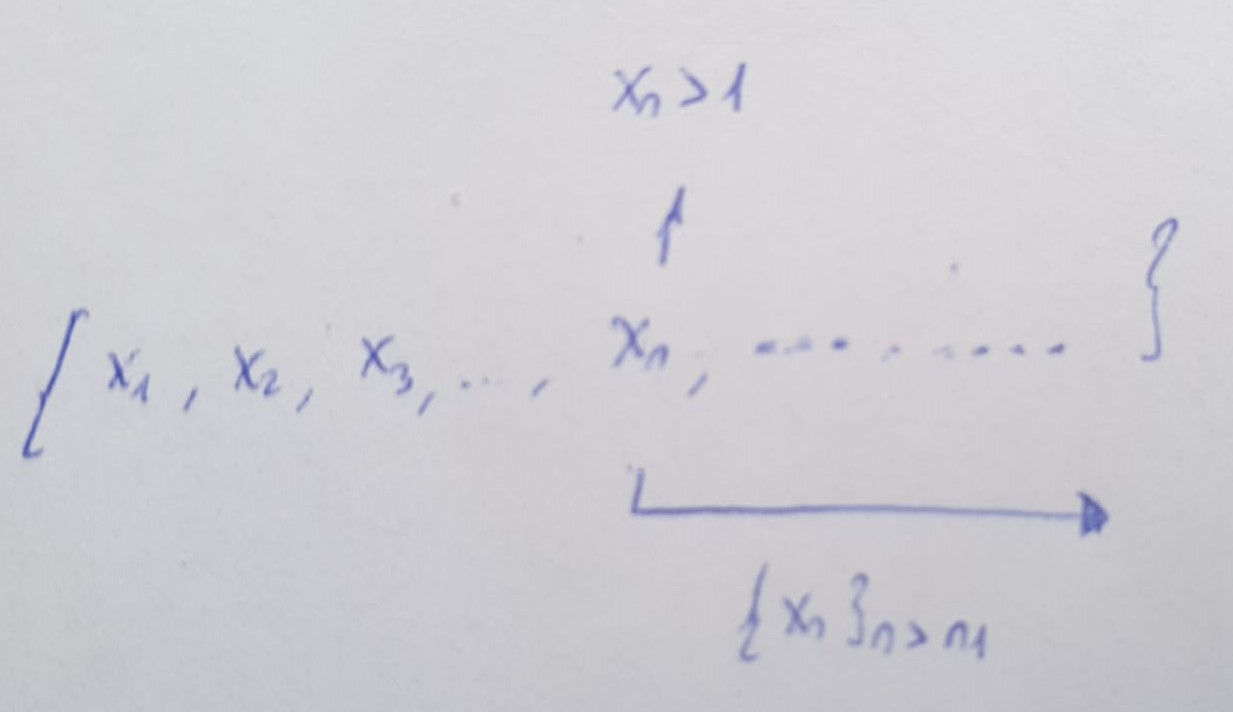
\includegraphics[scale=0.15]{proposicion subsucesiones}
\end{center}

Y este conjunto no estaría acotado porque si no toda la sucesión sería acotada superiormente y estamos suponiendo que no.

Ahora, sea $M=2$:
$$\exists n_2>n_1: x_{n_2}>2\Rightarrow \{x_n\}_{n>n_2}\mbox{ no acotado sup.}$$

Es decir, hemos buscado este $n_2$ dentro del intervalo que me quedaba más alla de $x_{n_1}$

Ahora, sea $M=3$:
$$\exists n_3>n_2: x_{n_3}>3\Rightarrow \{x_n\}_{n>n_3}\mbox{ no acotado sup.}$$


Por inducción se demuestra que $M=k\in \mathbb N: \exists n_k>n_{k-1}: x_{n_k}>k$. Por tanto, $\lim_{k\rightarrow \infty} x_{n_k}=\infty$ porque dado $M>0: \exists k_0\in \mathbb N: k_0>M\Rightarrow x_{n_{k_0}}>k_0>M\stackrel{k\geq k_0}{\Rightarrow} x_{n_k}>k>k_0\geq M$
\end{itemize}
\end{demo}

\begin{theo}[de Bolzano-Weirstrass]
Sea $\{x_n\}_{n=1}^\infty\subset R$ una sucesión acotada, entonces $\exists \{x_{n_k}\}_{k=1}^\infty$ subsucesión convergente.
\end{theo}
\begin{demo}
Supongamos que $a\leq x_n\leq b: \forall n\in \mathbb N$, utilizamos la siguiente notación: si $J$ es un intervalo y $n\in \mathbb N$, llamamos $I(J,n)=\{m\in \mathbb N :m>n: x_m\in J\}$, es decir, son los índices mayores que $n$ de manera que $x_m$ pertenece al conjunto.\par

En el fondo lo que vamos a hacer es partir el intervalo en dos, quedando dos posibles intervalos $J$. Entonces, en uno de esos dos, el conjunto $I(J,n)$ es infinito, es decir, hay infinitos índices. Y la construcción la vamos a hacer por inducción.

Sea $n_1=1$, para $J=[a, \frac{a+b}{2})$ o $J=(\frac{a+b}{2},b]$ el conjunto $I(J,1)$ es infinito, porque si no el conjunto formado por los índices de ambas posibilidades sería finito y hay infinitos índices. Llamamos $J_1$ a ese intervalo y llamamos $n_2$ al primer elemento de $I(J_1,n_1)$, por lo que: $n_2>n_1=1$.\par

Hacemos de nuevo lo mismo en $J_1$ tomándolo como nuevo intervalo del enunciado y dividiendo $J_1$ por su punto medio, quedando dos intervalos. En alguna de las dos mitades $I(J, n_2)$ es infinito. A esa mitad la llamamos $J_2$ y llamamos $n_3$ al primer elemento del conjunto $I(J_2,n_2)$ y por eso: $n_3>n_2>n_1=1$. Y de nuevo partimos $J_2$ por la mitad y seguimos...\par

Es decir, que por inducción construimos $\forall k\in \mathbb N: J_k\subset J_{k-1}$ donde $I(J_{k-1},n_{k-1})$ es infinito y $n_{k}$ es el primer elemento del mismo y por tanto $n_k>n_{k-1}$, por inducción se demuestra fácil.\par

Con ello hemos construido una familia de intervalos encajados $\{J_k\}_{k=1}^\infty$ y por el \textbf{teorema de intervalos encajados de Cantor} sabemos que $\bigcap_{k=1}^\infty J_k\neq \emptyset$ y de hecho es un único número: $\bigcap_{k=1}^\infty J_k=\{\varphi\}$ porque la longitud de $J_k$ es $l(J_k)=\frac{b-a}{2^k}\xrightarrow{k\rightarrow \infty} 0$\par

Veamos que $\{x_{n_k}\}_{k=1}^\infty$ converge a $\varphi$ ya que $\varphi\in J_k: \forall k$ y por construcción, como $n_k$ es el primer elemento de $I(J_{k-1},n_{k-1})$, entonces:
$$x_{n_k}\in J_{k-1}\wedge \varphi\in J_{k-1}\Rightarrow \left|x_{n_k}-\varphi\right|\leq \frac{b-a}{2^{k-1}}\Rightarrow \mbox{Sea }\varepsilon>0:\exists k_0, \forall k\geq k_0 : \left|x_{n_k}-\varphi\right|\leq \frac{b-a}{2^{k-1}}<\varepsilon$$
\end{demo}

\subsection{Sucesiones de Cauchy}
Supongamos que tenemos una sucesión de números reales $\{x_n\}_{n=1}^\infty\subset \mathbb R$ que converge a $l\in \mathbb R$, entonces:
$$\forall \varepsilon>0, \exists n_0\in \mathbb N: \forall n\geq n_0: |x_n-l|<\frac{\varepsilon}{2}$$
De este modo, sabemos que $n,m\geq n_0$ entonces $|x_n-x_m|=|x_n-l+l-x_m|\leq |x_n-l|+|x_m-l|< \frac{\varepsilon}{2}+\frac{\varepsilon}{2}=\varepsilon$, es decir, como ambos elementos de la sucesión están dentro del intervalo de centro el límite, la distancia entre ambos es menor que ese intervalo.

\begin{defi}[Sucesión de Cauchy]
Sea $\{x_n\}_{n=1}^\infty\subset \mathbb R$ una sucesión, se dice que es una \textbf{sucesión de Cauchy} si y sólo si:
$$\forall \varepsilon>0, \exists n_0\in \mathbb N: \forall n,m\geq n_0: |x_n-x_m|<\varepsilon$$
es decir, si la distancia entre cualesquiera de sus términos a partir de uno concreto es menor que el $\varepsilon$ prefijado.
\end{defi}

\begin{prop}
Las sucesiones convergentes son sucesiones de Cauchy.
\end{prop}

\begin{demo}
Precisamente el razonamiento inicial de este apartado demuestra este enunciado.
\end{demo}

\begin{prop}
Si una sucesión $\{x_n\}_{n=1}^\infty\subset \mathbb R$ es de Cauchy, entonces es acotada\footnote{Pero el recíproco no es cierto!!!, puede ser acotada pero no convergente}.\par
\end{prop}
\begin{demo}
Tomamos $\varepsilon=1: \exists n_0\in \mathbb N: \forall n,m\geq n_0: |x_n-x_m|<1$. En particular, $m=n_0$ y $n\geq n_0$:
$$|x_n|-|x_{n_0}|\leq |x_n-x_{n_0}|<1\Rightarrow |x_n|\leq |x_{n_0}|+1$$

Es decir, que todos los índices mayores de $n_0$ están acotados por el valor $|x_{n_0}|+1$. Ahora hay que ver los índices que no están comprendidos en la cantidad anterior: $\{|x_1|, \cdots, |x_{n_0-1}|\}$, pero como este es un conjunto finito, también está acotado por lo que escogiendo el máximo de ambas cotas, acota a todos los elementos de la sucesión.
\end{demo}

\begin{theo}[Completitud de $\mathbb R$]
Sea $\{x_n\}_{n=1}^\infty\subset \mathbb R$ una sucesión\footnote{Este resultado es falso en los números $\mathbb Q$} de Cauchy, entonces $\{x_n\}_{n=1}^\infty$ es convergente.
\end{theo}
\begin{demo}
Como la sucesión es de Cauchy, es acotada y entonces tiene una subsucesión convergente por el Teorema de Bolzano-Wiestrass, es decir, $\exists \{x_{n_k}\}_{k=1}^\infty$ convergente a $l\in \mathbb R$. Esto implica que: dado $\varepsilon>0, \exists k_0\in \mathbb N: k\geq k_0: |x_{n_k}-l|<\varepsilon$.\par

Veamos ahora que $\{x_n\}_{n=1}^\infty$ converge a $l$:
$$\mbox{Dado }\varepsilon>0, \exists k_0\in \mathbb N: k\geq k_0: |x_{n_k}-l|<\frac{\varepsilon}{2}\mbox{ y como es de Cauchy }\exists n_0\in\mathbb N: \forall m,n\geq n_0: |x_n-x_m|<\frac{\varepsilon}{2}\Rightarrow$$
$$\Rightarrow \exists k>k_0: n_k\geq n_0$$
Porque si no todos los subíncides posteriores a $k_0$ de la subsucesión estarían acotados y entonces no serían estrictamente crecientes.
Entonces, si $n\geq n_0$, medimos esta distancia:
$$|x_n-l|=|x_n-x_{n_k}+x_{n_k}-l|\leq \underbrace{|x_n-x_{n_k}|}_{< \frac{\varepsilon}{2}}+\underbrace{|x_{n_k}-l|}_{< \frac{\varepsilon}{2}}<\varepsilon$$
Porque como $k\geq k_0\Rightarrow |x_{n_k}-l|<\frac{\varepsilon}{2}$ y como $n,n_k\geq n_0\Rightarrow |x_n-x_{n_k}|<\frac{\varepsilon}{2}$

Por tanto, dado un $\varepsilon>0,\exists n_0\in \mathbb N: k\geq k_0\Rightarrow n\geq n_0: |x_n-l|<\varepsilon$
\end{demo}

\subsection{Límite inferior y superior de una sucesión}
Muchas veces tenemos sucesiones que no convergen a ningún valor concreto, pero que siempre oscilan entre varios valores posibles, por ejemplo, la sucesión $\{(-1)^n\}_{n=1}^\infty$. Es cierto que dicha sucesión no converge, pero si podemos acotar un conjunto sobre el que siempre se encuentran los posibles límites de cada subsucesión. Estas dos cotas del intervalo son precisamente las nociones de límite superior e inferior.

\begin{defi}
Sea $\{x_n\}\subset \mathbb R$ una sucesión acotada y denotamos $N\in \mathbb N$, entonces definimos las sucesiones:
$$a_N=\inf\{x_n: n\geq N\}\Rightarrow \{a_N\}\uparrow$$
$$b_N=\sup\{x_n: n\geq N\}\Rightarrow \{b_N\}\downarrow$$
\end{defi}

Ver la monotonía de ambas es sencillo, pero lo realmente relevante de ambas es:
$$\forall n\in \mathbb N: a_1\leq a_N\leq b_N\leq b_1$$
Por tanto, como son sucesiones monótonas y acotadas, el límite de ambas existen y es precisamente lo que llamamos \textbf{límite inferior y superior de una sucesión}.
\begin{defi}[Límite Inferior y Superior]
Sea $\{x_n\}\subset \mathbb R$ una sucesión acotada y $\{a_N\}$ y $\{b_N\}$ sus sucesiones superior e inferior, definimos el \textbf{límite superior e inferior} de la sucesión $\{x_n\}$ como:
$$\liminf_{n\rightarrow\infty}x_n=\lim_{N\rightarrow\infty}a_N$$
$$\limsup_{n\rightarrow\infty}x_n=\lim_{N\rightarrow\infty}b_N$$
\end{defi}

\begin{prop}
Sea $\{x_n\}_{n=1}^\infty$ una sucesión numérica, ésta converge si y sólo si su límite superior e inferior coinciden y ambos son el límite de la sucesión.
$$\lim_{n\rightarrow \infty}x_n=l\Leftrightarrow \liminf_{n\rightarrow\infty}x_n= \limsup_{n\rightarrow\infty}x_n=l$$
\end{prop}
\begin{demo}
\begin{itemize}
\item ``$\Leftarrow$'':
$$\forall N\in \mathbb N: a_N\leq x_N \leq b_N\Rightarrow a_N\xrightarrow{n\rightarrow\infty} l\leq x_N\leq n_N\xrightarrow{n\rightarrow\infty} l\Rightarrow x_N\xrightarrow{n\rightarrow\infty} l$$

\item ``$\Rightarrow$'':\par
Sea $l=\lim x_n$, entonces:
$$\forall \varepsilon>0: \exists n_0\in \mathbb N : \forall n\geq n_0: |x_n-l|<\varepsilon\Rightarrow l-\varepsilon <x_n<l+\varepsilon\Rightarrow l-\varepsilon \leq a_{n_0} \leq b_{n_0}\leq l+\varepsilon\stackrel{N\geq n_0}{\Rightarrow}$$
$$\Rightarrow l-\varepsilon \leq a_{n_0} \leq a_N \leq b_N \leq b_{n_0} \leq l+\varepsilon\Rightarrow l-\varepsilon \leq a_{n_0} \leq a_N \leq l\leq b_N \leq b_{n_0} \leq l+\varepsilon\Rightarrow \begin{cases}|a_N-l|<\varepsilon \\ |b_N-l|<\varepsilon \end{cases}\Rightarrow$$
$$\Rightarrow \lim_{n\rightarrow\infty}a_N=l= \lim_{n\rightarrow\infty}b_N$$
\end{itemize}
\end{demo}

\begin{prop}
Sea $s\in \mathbb{R}$ y $\{x_n\}_{n=1}^\infty\subset \mathbb{R}$ una sucesión numérica, entonces:
$$s > \limsup_{n\rightarrow\infty} x_n \Rightarrow \exists n_0 \in \mathbb{N} : \forall n \geq n_0: x_n<s$$
\end{prop}
\begin{demo}
Si tenemos que $\lim \{b_n\}\downarrow = l\Rightarrow \forall \varepsilon>0 : \exists n_0\in \mathbb N: \forall n\geq n_0: |b_n-l|<\varepsilon $ y en este caso podemos decir que $b_n-l<\varepsilon$. Ahora si vemos que $s>l$, entonces si escogemos $\varepsilon = |s-l|=s-l$, entonces por la definción de límite debe ocurrir que $b_n-l<s-l\Rightarrow b_n<s$ a partir de un cierto $n_0$.
\end{demo}

\begin{prop}
Sea $\{x_{n_k}\}_{k=1}^\infty\subset \{x_n\}_{n=1}^\infty\subset \mathbb{R}$ una subsucesión convergente, entonces su límite se encuentra entre el superior e inferior de la sucesión global.
$$ x_{n_k}\xrightarrow{n\rightarrow\infty}x_0 \Rightarrow \liminf x_n \leq x_0 \leq \limsup x_n$$
\end{prop}
\begin{demo}
$$\forall k\in \mathbb N: a_{n_k}\leq x_{n_k} \leq b_{n_k} \Rightarrow a\leq x_0 \leq b$$
\end{demo}

\begin{prop}
Sea $\{x_n\}_{n=1}^\infty \subset \mathbb{R}$ una sucesión numérica, entonces existe $\{x_{n_k}\}_{k=1}^\infty\subset \{x_n\}_{n=1}^\infty$ subsucesión convergente al límite inferior y $\{y_{n_k}\}_{k=1}^\infty\subset \{x_n\}_{n=1}^\infty$ subsucesión convergente al superior.
\end{prop}
\begin{demo}
Puede parecer que ya está demostrado en la propia definición de las sucesiones $a_N$ y $b_N$, pero en estos casos los índices no están ordenados, por lo que no son subsucesiones.
Si suponemos que $a$ es el límite de inferior, entonces sea $\varepsilon_1=1$ ocurre que $\exists n_1\in \mathbb N: a_1\leq x_{n_1}<a+1$ y por inducción podemos construir la siguiente sucesión: sea $\varepsilon_k= \frac{1}{k} : \exists n_k > n_k -1: a_{n_{k-1}}\leq x_{n_k}\leq a_{n_{k-1}}+\varepsilon_k$, por lo que se construye $\{x_{n_k}\}_{k=1}^\infty$ de manera que $a_{n_{k-1}}\leq x_{n_k}\leq a_{n_{k-1}}+\frac{1}{k}$ que vemos que por la regla del sandwich tiende a lo dicho.
\end{demo}

\begin{obs}
Con ello queda probado que, si definimos el conjunto de todos los puntos de $\mathbb{R}$ para los que existe alguna subsucesión convergente:
$$L=\{x_0\in \mathbb R: \exists \{x_{n_k}\}, \ x_{n_k}\xrightarrow{k\rightarrow \infty} x_0\}\}$$
entonces podemos redefinir ambos límites como:
$$\liminf_{n\rightarrow\infty}x_n=\inf L$$
$$\limsup_{n\rightarrow\infty}x_n=\sup L$$
\end{obs}

\subsection{Límites en el exponente}
Hasta ahora hemos demostrado que el límite se distribuye razonablemente en la suma y el producto de sucesiones. Sin embargo, una propiedad útil y que aún no hemos demostrado sería saber si también ocurre lo mismo con la exponencial, es decir, ¿si $x_n \xrightarrow{n\rightarrow \infty} x$ y $y_n \xrightarrow{n\rightarrow \infty} y$ la sucesión $x_n^{y_n} \xrightarrow{n\rightarrow \infty} x^y$?

\begin{theo}[Exponencial de exponente variable]
Sea $\{x_n\}_{n=1}^\infty$ una sucesión que converge a $x$ y $a>0$, entonces:
$$\lim_{n\rightarrow \infty} x_n = x \mbox{ y }a>0\Rightarrow \lim_{n\rightarrow\infty} a^{x_n}=a^x$$
\end{theo}
\begin{demo}
Veamos primero que si $\{x_n\}$ es monótona, entonces esto ocurre:
$$\{x_n\}\uparrow\Rightarrow a^{x_n}<a^{x_{n+1}}<a^x \Rightarrow \{a^{x_n}\} \uparrow$$
Además como $a^x>a^{x_n}:\forall n\in \mathbb N$, entonces está acotada, por lo que existe el supremo y además este es el límite de dicha sucesión. En consecuencia, por ser cota superior $a^x\geq \xi$ donde $\xi=\sup\{a^{x_n}\}$. Por la definición que se dió de exponencial real, el supremo de $a^{x_n}$ es $a^x$ por ser $x_n\in \mathbb R$.

Visto el caso de una función monótona, para una función cualquiera se tiene que como $x_n\xrightarrow{n\rightarrow\infty} x\Rightarrow a_N\xrightarrow{n\rightarrow\infty}x\xleftarrow{n\rightarrow\infty} b_N$ siendo ambos los límites superiores e inferiores descritos en el apartado anterior, así que como $\{b_N\}\downarrow$ y $\{a_N\}\uparrow$:
$$a_N\leq x_N\leq b_N \Rightarrow a^{a_N}\xrightarrow{n\rightarrow\infty}a^x\leq a^{x_N}\leq a^{b_N}\xrightarrow{n\rightarrow\infty}a^x\Rightarrow a^{x_N}\xrightarrow{N\rightarrow\infty}a^x$$
\end{demo}

\begin{theo}[Exponencial de base variable]
Sea $r\in \mathbb Q$ y $\{x_n\}_{n=1}^\infty$ una sucesión tal que $\forall n\in \mathbb N: x_n\geq 0$ y $\lim_{n\rightarrow\infty} x_n = x$, entonces:
$$\lim_{n\rightarrow\infty}x_n^{r} = x^r$$
\end{theo}
\begin{demo}
Comenzamos con el mismo razonamiento que para la demostración anterior, si $\{x_n\}\uparrow$ que converge a $x$ y $m\in \mathbb N$, entonces:
$$x_n\leq x_{n+1}\leq x\Rightarrow \sqrt[m]{x_n}\leq \sqrt[m]{x_{n+1}}\leq \sqrt[m]{x} \Rightarrow \{\sqrt[m]{x_n}\}\uparrow$$

Como es creciente y está acotada por $\sqrt[m]{x}$, su supremo existe y es el límite de dicha sucesión, en consecuencia, por ser cota superior $\xi\leq \sqrt[m]{x}$ donde $\xi=\sup\{\sqrt[m]{x_n}\}$. Veamos que el caso ``$<$'' no es posible:
$$\sqrt[m]{x_n}\leq \xi< \sqrt[m]{x}\Rightarrow x_n\xrightarrow{n\rightarrow\infty}x\leq \xi^m<x\xrightarrow{n\rightarrow\infty}x\Rightarrow \xi^m\xrightarrow{n\rightarrow\infty}x\Rightarrow \xi^m=x\Rightarrow \xi=\sqrt[m]{x}$$

En consecuencia, como $\{a_N\}\uparrow$ y $\{b_N\}\downarrow$, podemos acotar a cualquier sucesión convergente por esas dos y así demostrarlo para $\{x_n\}$ cualquiera que converja a $x$.
$$a_N\leq x_N\leq b_N\Rightarrow \sqrt[m]{a_N}\xrightarrow{n\rightarrow\infty}\sqrt[m]{x}\leq \sqrt[m]{x_n}\leq \sqrt[m]{b_N}\xrightarrow{n\rightarrow\infty}\sqrt[m]{x}\Rightarrow \sqrt[m]{x_N}\xrightarrow{n\rightarrow\infty}\sqrt[m]{x}$$

De ello se puede deducir, contando con la demostración anterior que si $m\in \mathbb Q$ entonces se cumple la proposición dada (contando con lo demostrado en la proposición anterior a este apartado).
\end{demo}

\begin{theo}[Exponencial de base y exponente variable]
Sean $\{x_n\}_{n=1}^\infty$ y $\{a_n\}_{n=1}^\infty$ sucesiones tal que $\lim_{n\rightarrow \infty}x_n = x$ y $\lim_{n\rightarrow\infty}a_n=a>0$, entonces:
$$\lim_{n\rightarrow\infty}a_n=a>0 \mbox{ y } \lim_{n\rightarrow\infty}x_n=x\Rightarrow \lim_{n\rightarrow\infty}a_n^{x_n}=a^x$$
\end{theo}
\begin{demo}
Para esta demostración necesitamos elaborar un poco el terreno la demostración final. Primero de todo tenemos que si $\lim_{n\rightarrow \infty} a_n=a\Rightarrow \lim_{n\rightarrow \infty}a_n^x=a^x$, cuya demostración utilizando las técnicas y resultados anteriores es trivial. Es fácil demostrar, teniendo en cuenta la definición de exponencial real que se dió, que si $x>0\Rightarrow a^x=\sup\{b^x: b<a\}=\inf\{c^x: a<c\}$ y del mismo modo que si $x<0\Rightarrow a^x=\inf\{b^x: b<a\}=\sup\{c^x: a<c\}$. Del mismo modo, es sencillo demostrar por casos que si $\{x_n\}$ es monótona convergente a $x$ y $a_n$ es monótona convergente a $a$, entonces $\lim_{n\rightarrow\infty} a_n^{x_n}=a^x$ con lo que basándonos en estos resultados tenemos que contando como $z_N$ la sucesión que tiende al límite inferior y $y_N$ la del superior:
$$z_N\leq a_N\leq y_N\Rightarrow z_N^{z'_n}\leq a_N^{z'_n}\leq a_N^{x_n}\leq a_N^{y'_n}\leq y_N^{y'_n}\Rightarrow z_N^{z'_n}\xrightarrow{n\rightarrow|\infty}a^x\leq a_N^{x_N}\leq y_N^{y'_n}\xrightarrow{n\rightarrow|\infty}a^x\Rightarrow a_N^{x_N}\xrightarrow{n\rightarrow|\infty}a^x$$
\end{demo}

\section{Series Numéricas}
El concepto nace de problemas como la suma de infinitos números. Para poder desarrollar dicha teoría, es necesario introducir (como en la mayoría de conceptos que tratan el infinito) el concepto de límite porque tal y como hemos definido la operación de la suma solo podemos sumar una cantidad finita de números. Tan grande como queramos, pero al fin y al cabo finita, es decir:
$$\sum_{i=1}^{n} x_i = x_1 + \cdots + x_n$$
Como nosotros necesitamos que esta cantidad sea infinita, una posible solución es calcular la suma hasta $n$. Las diferentes sumas hasta $n$, $n+1$, etc. conforman una sucesión de sumas y calcular la suma infinita sería lo mismo que calcular el límite de dicha sucesión, lo cual puedo hacerlo puesto que se ha reducido el problema al manejo de sucesiones.

\begin{defi}[Serie numérica]
Sea $\{x_n\}_{n=1}^\infty\subset \mathbb R$ una sucesión numérica, se define la \textbf{serie numérica} asociada como la sucesión de sumas parciales, es decir:
$$\{s_n\}_{n=1}^\infty: s_n = x_1 + x_2 + \ldots x_n = \sum_{k=1}^{n} x_k$$
Además, decimos que dicha \textbf{serie converge} si converge la sucesión de sumas parciales, es decir:
$$\sum_{n=1}^\infty x_n = \lim_{n\rightarrow\infty} s_n$$
\end{defi}

\begin{obs}
Las series pueden ``empezar'' en $n=0$, $n=2$ o $n=\gamma$ porque al fin y al cabo si la serie converge, empezar un poco más adelante no es tan importante. Esto se debe a que la suma hasta ese índice de comienzo será finita y como la que hemos escogido será convergente, la suma de ambas cantidades será finita, luego la sucesión desde el índice inicial es convergente en consecuencia.
\end{obs}

\begin{ej}
Tomamos la sucesión $ \displaystyle \sum_{n=0}^{\infty} \frac{1}{2^n}$ de forma que:
$$s_n =\frac{1}{2^0} + \frac{1}{2^1} + \ldots + \frac{1}{2^n} = \sum_{k=0}^{n} \frac{1}{2^k}$$
Calculamos ahora la suma finita hasta $n$ para conocer el término general de la sucesión $s_n$:
\begin{align*}
s_n &= \frac{1}{2^0} + \frac{1}{2^1} + \ldots + \frac{1}{2^n} \\
\frac{1}{2}\cdot s_n &= \frac{1}{2^1} + \frac{1}{2^2} + \ldots + \frac{1}{2^{n+1}} \\
s_n - \frac{1}{2}\cdot s_n &= \frac{1}{2}\cdot s_n = 1 - \frac{1}{2^{n+1}}
\end{align*}
$$s_n= 2\left(1 - \frac{1}{2^{n+1}}\right)$$
Luego en definitiva tenemos que:
$$\lim_{n \to \infty} s_n = \lim_{n \to \infty}  2\left(1 - \frac{1}{2^{n+1}}\right) = 2$$
\end{ej}

\subsection{Criterios de convergencia}
En ocasiones, como en el ejemplo anterior, será sencillo incluso calcular el valor concreto del límite de convergencia de una serie, pero en general no siempre será tan fácil. En su lugar, optaremos por determinar cuando una serie es o no convergente para que, en caso de requerirlo, perdamos nuestro tiempo calculando el límite (si existe) puesto que existen métodos matemáticos para aproximar o vislumbrar dicho límite.

\begin{theo}
Sea $\sum_{n=1}^\infty x_n$ una serie convergente\footnote{Es habitual encontrar la notación $\sum_{n=1}^\infty x_n < \infty$ para denotar que algo es convergente (también es usual en integrales)}, entonces la sucesión de términos que se suman tiende a $0$, es decir:
$$\sum_{n=1}^{\infty} x_n <\infty \Rightarrow \lim_{n \rightarrow \infty} x_n =0$$
\end{theo}
\begin{demo}
$$\sum_{n=1}^{\infty} x_n \mbox{ convergente } \Leftrightarrow \exists \lim_{n \to \infty} s_n = L: s_n = x_1 + x_2 + \ldots x_n = \sum_{k=1}^{n} x_k$$
De este modo, si tomamos estas dos sucesiones se verifica que:
$$\begin{cases}s_n \to L \\ s_{n-1} \to L\end{cases} \Rightarrow x_n = s_n - s_{n-1} \xrightarrow{n\rightarrow\infty} L-L = 0$$
\end{demo}

\begin{obs}
Cabe destacar que esto no significa que la sucesión de sumas parciales, es decir, la serie tienda a 0 ni tampoco que el recíproco sea cierto.
\end{obs}

\begin{ej}
\begin{enumerate}

\item $\sum n = 1 + 2 + 3 + \ldots$ no converge pues su $x_n = n \Rightarrow \lim_{n \to \infty} +\infty \neq 0 \Rightarrow \sum n$ es divergente

\item $\sum_{n=0}^{\infty} (-1)^n , s_n = 1 - 1 + 1 - 1 + \ldots + (-1)^n = \begin{cases} 0 \mbox { si $n$ impar } \\ 1 \mbox { si $n$ par } \end{cases} \Rightarrow $ no es convergente
\end{enumerate}
\end{ej}

\begin{ej}
Para ver que el recíproco no es cierto, tomamos de ejemplo la serie $\sum_{i = 1 }^{\infty} \frac{1}{n}$ llamada la serie armónica. Esta serie verifica que:
$$s_n = 1 + \frac{1}{2} + \frac{1}{3} + \ldots \frac{1}{n}\Rightarrow \forall n\in \mathbb N : s_n > 0$$
$$\{ s_n\}_{n=1}^\infty \uparrow \ \Rightarrow  0< s_n < s_{n+1}: \forall n \in \mathbb N$$
Cuando desarrollamos los sucesivos términos tenemos las siguientes desigualdades:
\begin{align*}
s_1 &= 1 \\
s_2 &= 1 + \frac{1}{2} \\
s_3 &=  1 + \frac{1}{2} + \frac{1}{3} \\
s_4 &= 1 + \frac{1}{2} + \frac{1}{3} + \frac{1}{4} > \frac{1}{4} + \frac{1}{4} + \frac{1}{4} + \frac{1}{4} = 1 \\
\vdots \\
s_8 &= 1 + \frac{1}{2} + \frac{1}{3} + \frac{1}{4} + \frac{1}{5} + \frac{1}{6} + \frac{1}{7} + \frac{1}{8} > 1 + \frac{1}{8} + \frac{1}{8} + \frac{1}{8} + \frac{1}{8} = 1 + \frac{1}{2} \\
\vdots \\
s_{16} &= 1 + \frac{1}{2} + \ldots \frac{1}{16} >1 + \frac{1}{2} + \frac{1}{2} \\
\vdots \\
s_{2^5} &= s_{2^4} + \frac{1}{2^4 + 1} + \ldots \frac{1}{2^4 + 2^4} > 1 + \frac{1}{2} + \frac{1}{2} + \frac{1}{2}
\end{align*}
Por tanto, es razonable pensar que la posible regla de inducción sea:
$$s_{2^n} > 1 + \frac{1}{2} + \ldots + \frac{1}{2} = 1 + \frac{n-2}{2}$$
así que para demostrarlo:
$$s_{2^{n+1}} = s_{2^n} + \frac{1}{2^n + 1} + \ldots + \frac{1}{2^n + 2^n} \overset{HI}{>} 1 +  \frac{n-2}{2} + \frac{1}{2^{n + 1}} + \ldots  + \frac{1}{2^{n + 1}} = 1+\frac{n-2}{2}+\frac{2^n}{2^{n+1}}= 1 + \frac{n-1}{2}$$
En consecuencia:
$$\lim_{n \to \infty} s_{2^n} = + \infty$$
Pero $\{s_n\}_{n=1}^\infty$ es monótona creciente $\Rightarrow \forall k, \exists n: s_k >s_{2^n}$, por tanto, $\lim_{n \to \infty} s_n = + \infty$; luego $\sum_{n=0}^{\infty} \frac{1}{n}$ es divergente.
\end{ej}

\begin{theo}[Criterio de Cauchy]
Sea $\sum_{n=1}^{\infty} x_n$ una serie numérica, ésta es convergente si y sólo la sucesión de sumas parciales es de Cauchy.
$$\forall \varepsilon >0 : \exists N\in \mathbb N: \forall n,m\geq N: |s_n-s_m|<\varepsilon$$
Es decir, para el caso de las series esto quiere decir que:
$$\forall \varepsilon >0 : \exists N\in \mathbb N: \forall n,m\geq N: \left|\sum_{m+1}^{n} x_k\right|<\varepsilon$$
\end{theo}
\begin{demo}
Si la serie en valor absoluto converge, entonces
$$\forall \varepsilon > 0, \exists N \in \mathbb{N}: n > m > N \Rightarrow |\sum_{m+1}^{n} |x_k| < \varepsilon$$
Pero es fácil ver la siguiente desigualdad:
$$\left|\sum_{m+1}^{n} x_k\right| \leq \sum_{m+1}^{n} \left|x_k\right|  < \varepsilon \overset{Cauchy}{\Rightarrow} \sum_{n=1}^{\infty} x_n \mbox{ es convergente }$$
\end{demo}

\begin{ej}
Como contraejemplo ejemplo para el recíproco se tiene la serie armónica alternada: $\sum_{n=1}^{\infty} \frac{(-1)^{n+1}}{n}$ que converge a $\ln(2)$, pero $\sum_{n=1}^{\infty} |x_n|$ que es la serie armónica diverge.
\end{ej}

\begin{coro}
Sea $\sum_{n=1}^{\infty} x_n$ una serie numérica cuyos términos no son todos necesariamente positivos, entonces:
$$\sum_{n=1}^{\infty} |x_n|\mbox{ converge}\Rightarrow \sum_{n=1}^{\infty} x_n\mbox{ converge}$$
\end{coro}

\begin{theo}[Criterio de comparación]
Sean $\{x_n\}_{n=1}^\infty, \{y_n\}_{n=1}^\infty \subset \mathbb{R}$ dos sucesiones numéricas que verifican que $\exists K \in \mathbb{N}: \forall n \geq K : 0 \leq x_n \leq y_n$, entonces:
\begin{align*}
\sum_{n=1}^{\infty} y_n \mbox{ converge} \Rightarrow \sum_{n = 1}^{\infty} x_n \mbox{ converge} & & \sum_{n=1}^{\infty} x_n\mbox{ diverge}\Rightarrow \sum_{n = 1}^{\infty} y_n \mbox{ diverge}
\end{align*}
\end{theo}
\begin{demo}
Si la serie es convergente, entonces ocurre que:
$$\forall \varepsilon > 0, \exists M \in \mathbb{N}: n \geq m \geq M \Rightarrow \sum_{m+1}^{n} y_k	< \varepsilon$$
Por tanto, si escogemos $M'=\min\{M,K\}$ entonces para $n>m\geq M'$ ocurre que:
$$0 \leq \sum_{m+1}^{n} x_n \leq \sum_{m+1}^{n} y_n < \varepsilon \Rightarrow \sum_{n=1}^{\infty} x_n\mbox{ es convergente}$$
\end{demo}

\begin{theo}[Criterio de comparación en el límite]
Sean $\{x_n\}_{n=1}^\infty$, $\{y_n\}_{n=1}^\infty$ dos sucesiones convergentes que verifican que $\exists n_0 \in \mathbb{N}: \forall n \geq n_0 : x_n , y_n \geq 0$, entonces si definimos
$$r = \lim_{n \rightarrow \infty} \frac{x_n}{y_n}$$
tenemos el siguiente criterio:
\begin{itemize}
\item $0< r <\infty$
$$\sum_{n=1}^{\infty} x_n \mbox{ converge} \Leftrightarrow \sum_{n=1}^{\infty} y_n \mbox{ converge}$$
\item $r = 0$
$$\sum_{n=1}^{\infty} y_n \mbox{ converge} \Rightarrow \sum_{n=1} ^{\infty} x_n \mbox{ converge}$$
\item $r= \infty$
$$\sum_{n=1}^{\infty} x_n \mbox{ converge} \Rightarrow \sum_{n=1} ^{\infty} y_n \mbox{ converge}$$
\end{itemize}
\end{theo}
\begin{demo}
Suponiendo que el límite es $r \neq 0$, entonces por la definición se verifica que:
$$\varepsilon = \frac{1}{2} r>0 \Rightarrow \exists K' \in \mathbb{N} : n \geq K' \Rightarrow | \frac{x_n}{y_n} - r|< \frac{1}{2} r : n \geq K' \Leftrightarrow \frac{1}{2} r <\frac{x_n}{y_n} < \frac{3}{2} r : n \geq K'$$
Si tomamos $\tilde{K} = \max \{K, K'\}$, entonces:
$$n \geq \tilde{K} \Rightarrow 0 <\frac{1}{2} r y_n < x_n < \frac{3}{2} r y_n $$
Supongamos en primer lugar que $\Sigma y_n$ es convergente, entonces:
$$\sum \frac{3}{2} y_n\mbox{ convergente} \overset{\mbox{Comparación}}{\Rightarrow} \sum x_n \mbox{ converge}$$
Por otro lado, si $\sum x_n$ converge, entonces:
$$\sum x_n\mbox{ convergente} \overset{\mbox{Comparación}}{\Rightarrow} \sum \frac{1}{2} y_n \mbox{ converge}\Rightarrow \sum y_n\mbox{ converge}$$
Supongamos ahora que $r=0$, entonces:
$$\forall \varepsilon >0: \exists K': n \geq K' \Rightarrow |\frac{x_n}{y_n}| < \varepsilon$$
De nuevo, tomando $\tilde{K} = \max \{K, K'\}$ y $n \geq \tilde{K}$, entonces:
$$0 < \frac{x_n}{y_n} < \varepsilon \Rightarrow 0 < x_n < \varepsilon y_n \Rightarrow$$
$$\Rightarrow \sum y_n \mbox{ converge }\Rightarrow \Sigma x_n \mbox{ converge}$$
\end{demo}

\subsection{Convergencia absoluta y condicional}
Estos conceptos toman gran relevancia sobre todo para el capítulo \nameref{sucesiones y series de funciones} puesto que permiten diferenciar entre unas más leves y otras condiciones más restrictivas de convergencia que ofrecen menos o más estabilidad en la misma.

\begin{defi}[Convergencia Absoluta y Condicional]
Sea $\sum_{n = 1}^{\infty} x_n$ una serie numérica, decimos que \textbf{converge absolutamente o es absolutamente convergente} si la serie de los valores absolutos es convergente, es decir:
$$\sum_{n = 1}^{\infty} x_n\mbox{ abs. conv.} \Leftrightarrow \sum_{n=1}^{\infty} |x_n|\mbox{ conv.}$$

Sea $\sum_{n = 1}^{\infty} x_n$ una serie numérica, decimos que \textbf{converge condicionalmente o es condicionalmente convergente} si es convergente pero no absolutamente convergente, es decir:
$$\sum_{n = 1}^{\infty} x_n\mbox{ cond. conv.} \Leftrightarrow \sum_{n=1}^{\infty} |x_n|\mbox{ div. y } \sum_{n = 1}^{\infty} x_n \mbox{ conv.}$$
\end{defi}

\begin{theo}[Criterio de la Raíz y del Cociente]
\begin{itemize}
\item \underline{\textbf{Criterio de la raíz}}:

	Sea $\{x_n\}_{n=1}^\infty$ una sucesión numérica, entonces:
	\begin{itemize}
	\item $\exists r\in (0,1): \forall n\geq K: |x_n|^\frac{1}{n}\leq r \Rightarrow  \sum_{n=1}^{\infty} x_n$ abs. conv.
	\item $\exists K \in \mathbb N: \forall n\geq K: |x_n|^\frac{1}{n} \geq 1 \Rightarrow \sum_{n=1}^{\infty} x_n$ div.
	\end{itemize}
	En la práctica, utilizamos su corolario para poder determinar la convergencia en las series:
$$\exists r \in \mathbb R: r= \lim_{n \rightarrow \infty} |x_n|^{\frac{1}{n}} \begin{cases}
0 \leq r < 1 &\Rightarrow \sum x_n \mbox{ abs. conv.} \\ r>1 &\Rightarrow \sum x_n\mbox{ div.}\\ r=1 &\Rightarrow ???\end{cases}$$

	
\item \underline{\textbf{Criterio del cociente}}:
	
	Sea $\{x_n\}_{n=1}^\infty$ una sucesión numérica tal que $\forall n \in \mathbb{N} : x_n \neq 0$, entonces:
	\begin{itemize}
	\item $\exists r\in (0,1): \forall n\geq K: \left|\frac{x_{n+1}}{x_n}\right| \leq r \Rightarrow \sum x_n \mbox{ abs. conv. }$
	\item $\exists K \in \mathbb N: \forall n\geq K: \left|\frac{x_{n+1}}{x_n}\right| \geq 1 : \forall n \geq K \Rightarrow \sum x_n \mbox{ div. } $
	\end{itemize}
	En la práctica, utilizamos su corolario para poder determinar la convergencia en las series:
	$$\exists r\in \mathbb R: r = \lim_{n \rightarrow \infty} \left|\frac{x_{n+1}}{x_n}\right|\Rightarrow \begin{cases} 0<r<1 \Rightarrow \sum_{n=1}^{\infty} x_n \mbox{ abs. conv.} \\ r>1 \Rightarrow  \sum_{n=1}^{\infty} x_n \mbox{ div. } \\ r = 1 \Rightarrow ??? \end{cases}	$$
\end{itemize}
\end{theo}
\begin{demo}
\begin{itemize}
\item Criterio de la raíz:

El primer punto del criterio es equivalente a decir que $|x_n| \leq r^n : \forall n \geq K$, pero ocurre que:
$$0 \leq r < 1 \Rightarrow \sum_{n=1}^{\infty} r^n \mbox{ es convergente }\overset{\mbox{Comparación}}{\Rightarrow} \Sigma |x_n| \mbox{ es convergente}$$
El segundo punto es trivial, porque:
$$|x_n|^{\frac{1}{n}} \geq 1 : \forall n \geq K \Rightarrow \lim_{n \to  \infty} |x_n| \neq 0 \Rightarrow \sum_{n=1}^\infty x_n \mbox{ es divergente}$$

\item Criterio del Cociente:

Para empezar, si consideramos el primer punto tenemos que $ |x_{n+1} | \leq r |x_n|: \forall n \geq K $, luego vemos que para los sucesivos términos:
$$\begin{cases}|x_{k+1}| \leq r |x_k| \\ |x_{k+2}|\leq r |x_{k+1}| \leq r^2 |x_k| \\ \vdots \\ |x_{k+m}| \leq r^m |x_k| : \forall m = 0,1,2,\ldots \end{cases}$$
Luego podemos reescribir que:
$$|x_{k+m}| \leq r^{k+m} \underbrace{\frac{|x_k|}{r^k}}_a : \forall m = 0,1,2,\ldots$$
Y si consideramos la sucesión a partir del término $k-esimo$ tenemos que:
$$|x_n| \leq a r^n : \forall n \geq k$$
Pero $\sum_{n=1}^{\infty} a r^n$ es convergente, y por el criterio de comparación $\Rightarrow \sum_{n=1}^{\infty} |x_n|$ es convergente

Si consideramos ahora el segundo punto tenemos que $|x_{n+1}| \geq |x_n|: \forall n \geq K $, luego entonces:
$$\Rightarrow |x_n| \geq |x_k|: \forall n \geq K: x_n \cancel{\rightarrow} 0 \Rightarrow  \sum_{n=1}^\infty x_n \mbox{ diverge}$$
\end{itemize}
\end{demo}

\begin{theo}[Criterio de la integral]
Sea $f:[0, \infty)\rightarrow \mathbb R$ una función integrable, $f(x)\geq 0 $, decreciente y cuyo $\lim_{x \rightarrow \infty} f(x) = 0$, entonces decimos que:
$$\int_{0}^{\infty} f(x) \dif{x} \mbox{ converge} \Leftrightarrow \sum_{n = 1 }^{\infty} f(n)\mbox{ converge}$$
\end{theo}
\begin{demo}
La demostración y explicación de este resultado se encuentra en el tema dedicado a las integrales, concretamente en la sección \nameref{Integrales Impropias}.
\end{demo}

\begin{theo}[Criterio de Leibnitz]
Sea $\{x_n\}_{n=1}^\infty$ una sucesión numérica que verifica:
\begin{itemize}
\item $\forall n \in \mathbb{R}: x_n > 0$
\item $\{x_n\}_{n=1}^\infty \downarrow$
\item $\lim_{n \rightarrow \infty} x_n = 0$
\end{itemize}
entonces se cumple que:
$$\sum_{n=1}^{\infty} (-1)^{n+1}x_n\mbox{ es convergente}$$
\end{theo}
\begin{demo}
Sea $s_n = x_1 - x_2 + \ldots + (-1)^{n+1}x_n = \sum_{k=1}^{n} (-1)^{k+1} x_k$. Vamos a tomar la sucesión de los pares:
$$s_{2n} = \underbrace{x_1 - x_2}_{\geq 0} + \underbrace{x_3 - x_4}_{\geq 0} + \ldots + \underbrace{x_{2n-1} - x_{2n}}_{\geq 0} \geq 0$$
Además, también se verifica que:
$$s_{2n + 2} = s_{2n} + \underbrace{x_{2n + 1} - x_{2n + 2}}_{\geq 0} \geq s_{2n} \Rightarrow \{s_{2n}\}_{n=1}^\infty\uparrow$$
Incluso es acotada:
$$s_{2n} = x_1 \underbrace{-x_2 + x_3}_{\leq 0 } \underbrace{- x_4 + x_5 }_{\leq 0}- \underbrace{\ldots + x_{2n-1}}_{\leq 0} - x_{2n}\leq x_1 - x_{2n} \leq x_1 $$
Como es una sucesión acotada y creciente:
$$\exists L = \lim_{n \to \infty} s_{2n}$$

Ahora vamos a ver las sucesión de los impares:
$$s_{2n+1} =\underbrace{x_1 - x_2}_{\geq 0} + \underbrace{x_3 - x_4}_{\geq 0} + \ldots +\underbrace{x_{2n-1} - x_{2n}}_{\geq 0} + x_{2n+1} \geq 0$$
Del mismo modo:
$$s_{2n+3} = s_{2n+1} \underbrace{-x_{2n + 2} + x_{2n + 3}}_{\leq 0} \leq s_{2n+1} \Rightarrow  \{s_{2n+1}\}_{n=1}^\infty \downarrow$$
Y también ocurre que: 
$$s_{2n+1} \geq 0 \Rightarrow \exists L' = \lim_{n \to \infty} s_{2n+1}$$

En consecuencia, probamos ahora que ambos límites coinciden:
$$s_{2n} = s_{2n-1} - x_{2n} \Rightarrow L = L' + 0 \Rightarrow L = L'$$

Por tanto, ahora podemos concluir que entonces el límite de la serie es el propio $L$ porque al ser límite de la subsucesión de los términos pares e impares ocurre:
$$\begin{cases} \varepsilon > 0, \exists N : \forall n \geq N \Rightarrow |s_{2n} - L|<\varepsilon \\ \varepsilon > 0, \exists N' : \forall n \geq N' \Rightarrow |s_{2n+1} - L|<\varepsilon\end{cases} $$
Si escogemos como constante $\bar{N} = \max\{N, N'\}$, entonces se tiene que cumple ambas definiciones simultáneamente:
$$n \geq \bar{N} \Rightarrow \begin{cases} |s_{2n} - L|<\varepsilon & n = 2k \\ |s_{2n+1} - L|<\varepsilon & n = 2k+1\end{cases} \Rightarrow \forall k \geq \bar{N}: |s_k-L|<\varepsilon$$
\end{demo}

\begin{theo}[Criterio de Condensación de Cauchy]
Sea $\{x_n\}_{n=1}^\infty \downarrow$ una sucesión decreciente, $\forall n \in  \mathbb{N} : x_n > 0$ y $x_n \xrightarrow{n\rightarrow \infty} 0$, entonces:
$$\sum_{n=1}^{\infty} x_n \mbox{ converge } \Leftrightarrow \sum_{n=1}^{\infty} 2^n x_{2^n} \mbox{ converge }$$
\end{theo}
\begin{demo}
Sea $s_n = x_1 + x_2 + \ldots + x_n$, tomamos por ejemplo $s_{16}$:
$$s_{16} = x_1 + x_2 + x_3 + x_4 + x_5 + x_6 + x_7 + x_8 + \ldots + x_{16}$$
Acotamos la suma parcial superiormente:
$$s_{16} = x_1 + \underbrace{x_2 + x_3}_{ \leq x_2 + x_2} + \underbrace{x_4 + x_5 + x_6 + x_7}_{\leq 4x_4} + \underbrace{x_8 + \ldots +}_{\leq 8x_8} x_{16} \leq x_1 + 2x_2 + 2^2 x_{2^2} + 2^3 x_{2^3} + x_{2^4}$$
Luego por inducción podemos concluir que:
$$s_{2^n} \leq x_1 + 2x_2 + 2^2 x_{2^2} + \ldots + 2^{n-1} x_{2^{n-1}}+ x_{2^n}$$
Acotamos la suma parcial inferiormente:
$$s_{16} = x_1 + x_2 +\underbrace{ x_3 + x_4}_{\geq 2x_4} + \underbrace{ x_5 + x_6 + x_7 + x_8}_{\geq 4x_8} + \underbrace{ x_9 + \ldots + x_{16}}_{\geq 8x_{16}}\geq x_1 + x_2 + 2 x_{2^2} + 2^2 x_3 x_{2^3} +  2^3 x_{2^4} \geq$$
$$\geq \frac{1}{2}  x_1 + \frac{1}{2} x_2 + \frac{1}{2} 2 x_{2^2} + \frac{1}{2} 2^2 x_3 x_{2^3} + \frac{1}{2} 2^3 x_{2^4} =\frac{1}{2} (x_1 + 2x_2 + 2^2 x_{2^2} + + 2^3 x_3 x_{2^3} + + 2^4 x_{2^4})$$
Así que tenemos acotada por arriba y por abajo la subsucesión de los términos que son potencia de 2:
$$\frac{1}{2} (x_1 + 2x_2 + 2^2 x_{2^2} + + 2^3 x_3 x_{2^3} + + 2^4 x_{2^4}) \leq s_{2^4} \leq x_1 + 2x_2 + 2^2 x_{2^2} + + 2^3 x_3 x_{2^3} + + 2^4 x_{2^4}$$
Demostrado para todos por inducción se tiene que:
$$\frac{1}{2} (x_1 + 2x_2 + 2^2 x_{2^2} + \ldots + 2^n x_{2^n}) \leq s_{2^n} \leq x_1 + 2x_2 + 2^2 x_{2^2} + \ldots + 2^n x_{2^n}$$

Si consideramos la serie $ \sum_{n=1}^{\infty} 2^n x_{2^n} $, entonces la subsucesión de $\{s_n\}$ formada por los términos $x_{2^n}$ está acotada por 
esta serie. De este modo, si esta converge, entonces la subsucesión $\{s_{2^n}\}$ está acotada y, por tanto, la sucesión $\{s_n\}$ converge. De forma análoga, si la sucesión $\{s_n\}$ converge, entonces la subsucesión $\{s_{2^n}\}$ converge y como esta acota a la serie que habíamos definido multiplicada por un medio, entonces la serie converge.
\end{demo}

\begin{obs}
Este criterio resulta muy útil para decidir la convergencia de sucesiones en las que intervengan logaritmos, pues al tener $\ln (n)$ y sustituir $\ln (2^k)$ podemos sacar $k$ fuera para que nos quede una expresión más sencilla.
\end{obs}


\chapter{Funciones Continuas}
Las funciones son el concepto central y fundamental del análisis de variable real y sobre ellas se sustenta la mayor parte de la teoría que se analiza. Si las funciones de por sí ya revisten gran importancia, las posibilidades que nos ofrecen las continuas, por la cantidad de resultados beneficiosos demostrados para las mismas, hacen que trabajar con dichas funciones sea muy productivo y eficiente. Por ello, merece la pena hacer un estudio exhaustivo de las mismas para manejar bien las posibilidades que nos ofrecen.

\section{Concepto de Límite}
En primer lugar, el objetivo será definir el concepto básico de límite. Dicho concepto tiene una idea intuitiva muy similar al visto en las sucesiones, sin embargo, la definición formal del mismo dista mucho de ser la misma. En este apartado se van a ver las propiedades fundamentales para trabajar con límites y operar con los mismos.

\subsection{Topología fundamental}
Para poder comprender las nociones de límite, es necesario dar unas nociones básicas de topología para simplificar y comprender en profundidad los enunciados sobre límites que se van a dar posteriormente.

\begin{defi}[Punto de Acumulación]
Sea $D\subset \mathbb R$, decimos que $x_0\in \mathbb R$ es un \textbf{punto de acumulación de D} si y sólo si:
$$\forall \delta>0: \exists d\in D: d\in (x_0-\delta, x_0+\delta)\setminus\{x_0\}$$
Denotamos al conjunto\footnote{Nótese que $D'\nsubseteq D$.} de puntos de acumulación de $D$ por $D'$.
\end{defi}

\begin{obs}
La definición anterior viene a decir que para todo entorno alrededor de $x_0$ podemos encontrar otros puntos de $D$ que no sean dicho $x_0$, luego también podemos verlo como:
$$D\cap \left((x_0-\delta, x_0+\delta)\setminus \{x_0\}\right)\neq \emptyset$$
\end{obs}

\begin{ej}
$D=(0,1)\cup (1,2]\cup \{3\}$, si dejamos puesto el propio número diríamos que este punto es punto de acumulación y vemos claramente por el dibujo que no es cierto.
\end{ej}

\begin{center}
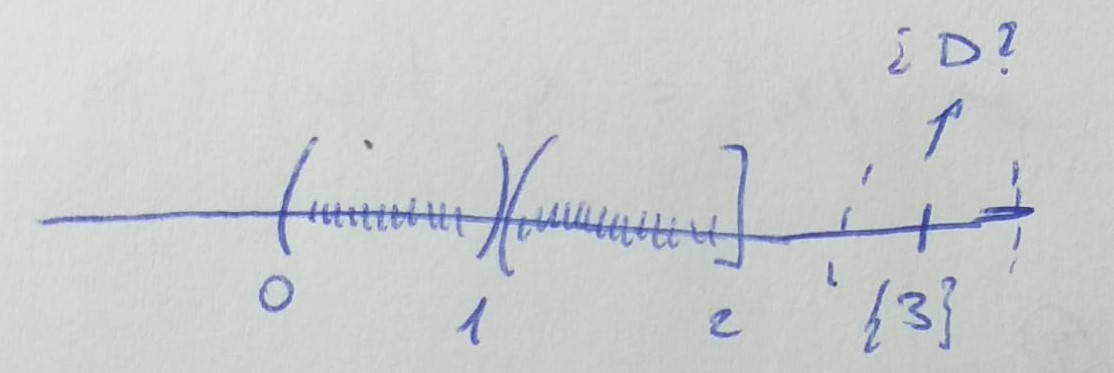
\includegraphics[scale=0.20]{Cauchy 2}
\end{center}

\begin{defi}[Punto Aislado]
Sea $D\subset \mathbb R$ y $x_0\in D$, decimos que es un \textbf{punto aislado} de $D$ si no es de acumulación:
$$\exists \delta >0 : D\cap \left((x_0-\delta, x_0+\delta)\mbox{\textbackslash} \{x_0\}\right)= \emptyset$$
\end{defi}

\begin{ej}
En el ejemplo de arriba, 3 es un punto aislado. Todos los puntos de D \textbf{o son de acumulación o son aislados}.
\end{ej}

\begin{prop}
Sea $D\subset \mathbb R$ y $x_0\in D$, entonces:
$$x_0 \in D' \Leftrightarrow \exists \{x_n\}_{n=1}^\infty \subset D: \lim_{n\rightarrow \infty} x_n=x_0\mbox{ y } \forall n \in \mathbb{N} : x_n \neq x_0$$
\end{prop}
\begin{demo}
\begin{itemize}
\item ``$\Rightarrow $'':\par
Como sabemos que es un punto de acumulación, entonces tomamos $\delta=\frac{1}{n}: \forall n\in \mathbb N$, entonces $D\cap \left((x_0-\frac{1}{n}, x_0+\frac{1}{n})\mbox{\textbackslash} \{x_0\}\right)\neq \emptyset$. Esto implica que:
$$\exists x_n\in D: x_n\in \left(x_0-\frac{1}{n}, x_0+\frac{1}{n}\right): x_n\neq x_0\Rightarrow 0\stackrel{x_n\neq x_0}{<}|x_n-x_0|<\frac{1}{n} \stackrel{ReglaSandwich}{\Rightarrow} \lim_{n\rightarrow \infty} |x_n-x_0|=0\Rightarrow$$
$$\Rightarrow \lim_{n\rightarrow \infty} (x_n-x_0)=0\Rightarrow \lim_{n\rightarrow \infty} x_n=x_0$$

\item ``$\Leftarrow$'':\par
Como sabemos que existe dicha sucesión entonces sabemos que siendo $\delta >0$, entonces $\exists n_0\in \mathbb N: \forall n\geq n_0: |x_n-x_0|<\delta\Leftrightarrow x_n\in (x_0-\delta , x_0+\delta)$ y podemos decir además que como $x_n\neq x_0$, entonces:
$$x_n\in (x_0-\delta , x_0+\delta)\mbox{\textbackslash} \{x_0\}\stackrel{x_n\in D}{\Rightarrow} D\cap\left((x_0-\delta , x_0+\delta)\mbox{\textbackslash} \{x_0\}\right) \neq \emptyset$$
\end{itemize}
\end{demo}

\subsection{Límite y propiedades}
El concepto intuitivo que queremos expresar es que si tenemos $D\subset R: D\neq \emptyset$ y $f: D\longrightarrow \mathbb R$, entonces queremos formalizar que si $x_0\in \mathbb R$ y $x\in D$ y $x\sim x_0$, entonces $f(x)\sim l: l\in \mathbb R$. El número $x_0$ es un punto de acumulación\footnote{Es notable decir que NO tiene por qué estar en D} para que siempre tenga cerca números del conjunto.

\begin{defi}[Límite de una Función]
Sea $D\subset \mathbb R: D\neq \emptyset$, $f:D\longrightarrow \mathbb R$ una función real y $x_0\in D'$, entonces decimos que $l\in \mathbb R$ es el \textbf{límite de $f(x)$ cuando $x$ tiende a $x_0$} si y sólo si:
$$\lim_{x\rightarrow x_0} f(x) = l \Leftrightarrow \forall \varepsilon>0, \exists \delta>0 : x\in D\cap \left((x_0-\delta, x_0+\delta)\mbox{\textbackslash} \{x_0\}\right)\Rightarrow f(x)\in (l-\varepsilon, l+\varepsilon)$$
\end{defi}

\begin{obs}
Es decir, estamos diciendo que escogido un intervalo sobre el eje de las y, podemos encontrar una amplitud $\delta$ para que un entorno de dicha amplitud en el eje de las $x$ esté contenido completamente en el intervalo tubular de las y prefijado con anterioridad.

\begin{center}
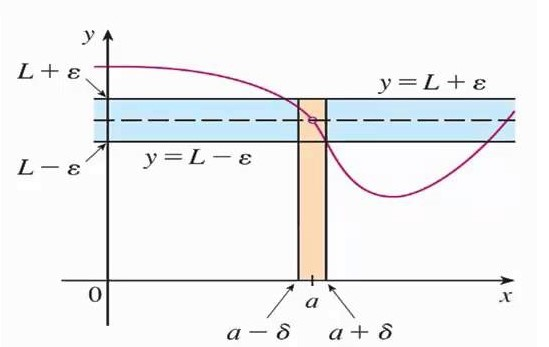
\includegraphics[scale=0.40]{limite}
\end{center}

De forma más simplificada y habitual, podemos escribir dicha definición como:
$$\forall \varepsilon>0, \exists \delta>0 : x\in D, \ 0\stackrel{x\neq x_0}{<}|x-x_0|<\delta\Rightarrow |f(x)-l|<\varepsilon$$
\end{obs}

\begin{prop}[Caracterización del Límite]
Sea $D\subset \mathbb R$, $f:D\longrightarrow \mathbb R$ y $x_0\in D'$, entonces:
\begin{enumerate}
\item $\lim_{x\rightarrow x_0} f(x)=l\in \mathbb R \Leftrightarrow \forall \{x_n\}_{n=1}^\infty\subset D, \ x_n\neq x_0: x_n\xrightarrow{n\rightarrow \infty} x_0\Rightarrow 	f(x_n)\xrightarrow{n\rightarrow \infty} l$

\item $\exists \lim_{x\rightarrow x_0} f(x)\Rightarrow \exists! \lim_{x\rightarrow x_0} f(x)$
\end{enumerate}
\end{prop}
\begin{demo}
\begin{enumerate}
\item Comprobamos que se dan ambas implicaciones:
	\begin{itemize}
	\item ``$\Rightarrow$'': \par
	Sea $\{x_n\}_{n=1}^\infty\subset D$ y $x_n\neq x_0: \forall n\in \mathbb N$ y tal que $x_n\xrightarrow{n\rightarrow \infty} x_0$, veamos que $f(x_n)\xrightarrow{x_n\rightarrow \infty} l$:
	
	Como sabemos que $l$ es el límite, entonces:
	$$\mbox{Sea }\varepsilon>0,\mbox{ entonces } \exists \delta >0: x\in D\cap \left((x_0-\varepsilon, x_0+\varepsilon)\mbox{\textbackslash} \{x_0\}\right)\Rightarrow f(x)\in (l-\varepsilon, l+\varepsilon)\Rightarrow$$
	$$\Rightarrow \exists n_0\in \mathbb N: \forall n\geq n_0: x_n \in (x_0-\delta, x_0+\delta)\stackrel{x_n\neq x_0}{\Rightarrow}x_n \in (x_0-\delta, x_0+\delta)\mbox{\textbackslash}\{x_0\}\stackrel{x_n\in D}{\Rightarrow}$$
	$$\Rightarrow  x_n \in D\cap\left((x_0-\delta, x_0+\delta)\mbox{\textbackslash}\{x_0\}\right)\Rightarrow f(x_n)\in (l-\varepsilon, l+\varepsilon)\Leftrightarrow |f(x_n)-l|<\varepsilon$$
	
	\item ``$\Leftarrow$'': supongamos que $l$ no es el límite:
	$$\exists \varepsilon>0, \forall \delta>0: \exists x\in D\cap \left((x_0-\delta, x_0+\delta)\mbox{\textbackslash} \{x_0\}\right): f(x)\notin (l-\varepsilon, l+\varepsilon)\Leftrightarrow |f(x)-l|>\varepsilon$$
	
	Entonces tomamos ahora $\delta=\frac{1}{n}$, entonces:
	$$\forall n\in \mathbb N, \exists x_n\in D\cap \left((x_0-\frac{1}{n}, x_0+\frac{1}{n})\mbox{\textbackslash} \{x_0\}\right): |f(x_n)-l|>\varepsilon$$
	Entonces los números anteriores forman una sucesión que: $\{x_n\}_{n=1}^\infty\subset D: x_n\neq x_0: \forall n\in \mathbb N: |x_n-x_0|<\frac{1}{n}\Rightarrow \lim_{n\rightarrow\infty} x_n=x_0$, pero $\{f(x_n)\}_{n=1}^\infty \mbox{ }\stackrel{n\rightarrow\infty}{\cancel{\longrightarrow}}\mbox{ } l\Rightarrow$ \#	
	\end{itemize}
	
\item Supongamos que hay dos $l_1$ y $l_2$ que son distintos, por lo que $l_1<l_2$, entonces:

\begin{center}
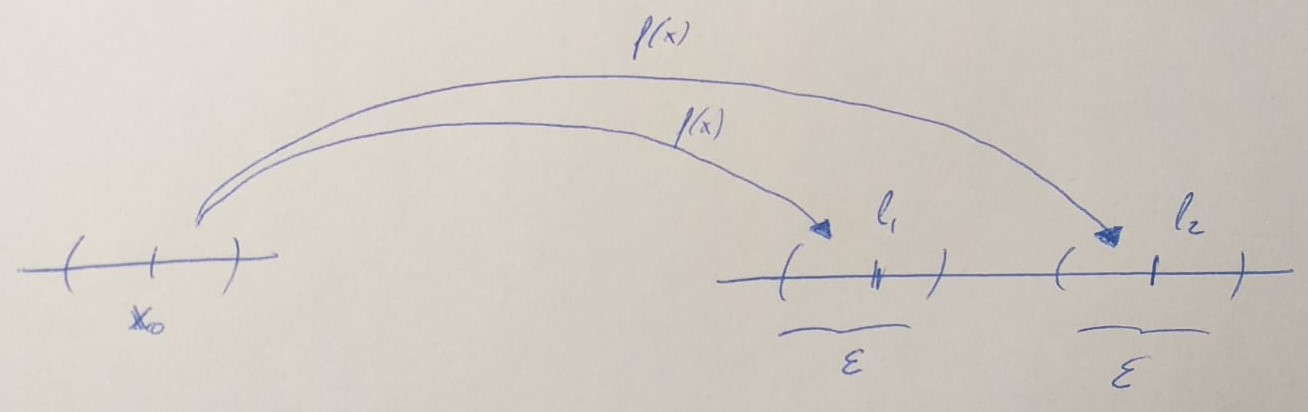
\includegraphics[scale=0.30]{limite doble}
\end{center}

En el fondo no estamos haciendo más que demostrar que si dichos entornos son disjuntos no se puede cumplir porque las funciones no pueden asignar dos imágenes al mismo punto del dominio.

Tomamos $\varepsilon=\frac{l_2-l_1}{2}$, lo que implica que:
$$\exists \delta_1>0: x\in D\cap \left((x_0-\delta_1, x_0+\delta_1)\mbox{\textbackslash}\{x_0\}\right) \Rightarrow f(x)\in (l_1-\varepsilon, l_1+\varepsilon)$$
$$\exists \delta_2>0: x\in D\cap \left((x_0-\delta_2, x_0+\delta_2)\mbox{\textbackslash}\{x_0\}\right) \Rightarrow f(x)\in (l_2-\varepsilon, l_2+\varepsilon)$$
Si tomamos $\delta=min\{\delta_1, \delta_2\}$, entonces:
$$x\in D\cap \left((x_0-\delta, x_0+\delta)\mbox{\textbackslash}\{x_0\}\right) \Rightarrow f(x)\in (l_1-\varepsilon, l_1+\varepsilon)\cap (l_2-\varepsilon, l_2+\varepsilon)$$
Y es fácil probar que: $(l_1-\varepsilon, l_1+\varepsilon)\cap (l_2-\varepsilon, l_2+\varepsilon)\neq \emptyset$
\end{enumerate}
\end{demo}

\begin{theo}[Operaciones con Límites]
Sea $D\subset \mathbb R$, $f,g: D\longrightarrow \mathbb R$ y $x_0\in D'$. Suponemos $\lim_{x\rightarrow x_0}f(x)=l$ y $\lim_{x\rightarrow x_0}g(x)=m$, entonces:
\begin{enumerate}
\item $\lim_{x\rightarrow x_0}(g(x)+f(x))=m+l$
\item $\lim_{x\rightarrow x_0}(a\cdot f(x))=a\cdot l$
\item $\lim_{x\rightarrow x_0}(f(x)\cdot g(x))=l\cdot m$
\item Si $m\neq 0$, entonces: $\lim_{x\rightarrow x_0}\frac{f(x)}{g(x)}=\frac{l}{m}$
\end{enumerate}
\end{theo}
\begin{demo}
\begin{enumerate}
\item Dado $\varepsilon>0$, tenemos que encontrar un $\delta$ de manera que $|f(x)+g(x)-(l+m)|<\varepsilon$:
$$|f(x)+g(x)-(l+m)|=|f(x)-l+g(x)-m|\leq |f(x)-l|+|g(x)-m|$$

Por saber como hipótesis que los límites de ambas funciones son $l$ y $m$, entonces:
$$\mbox{Dado }\varepsilon>0:\begin{cases} \exists \delta_1>0: x\in D\cap \left((x_0-\delta_1, x_0+\delta_1)\mbox{\textbackslash}\{x_0\}\right)\Rightarrow |f(x)-l|<\frac{\varepsilon}{2}\\ \exists \delta_2>0: x\in D\cap \left((x_0-\delta_2, x_0+\delta_2)\mbox{\textbackslash}\{x_0\}\right)\Rightarrow |g(x)-m|<\frac{\varepsilon}{2}\end{cases}$$
Luego si tomamos como $\delta=min\{\delta_1,\delta_2\}$ se tiene que se verifican ambas cosas:
$$\forall \varepsilon>0: \exists \delta>0: 0<|x-x_0|<\delta\Rightarrow |f(x)-l|+|g(x)-m|<\frac{\varepsilon}{2}+\frac{\varepsilon}{2}=\varepsilon$$

\item Queremos probar que dado $\varepsilon>0$ queremos encontrar un $\delta$ que cumpla que $|af(x)-al|<\varepsilon$:
$$|af(x)-al|=|a|\cdot |f(x)-l|$$

Como sabemos que $l$ es el límite de $f(x)$, entonces
$$\mbox{Dado }\varepsilon>0: \exists \delta>0: 0<|x-x_0|<\varepsilon\Rightarrow |f(x)-l|<\frac{\varepsilon}{|a|}$$
Luego se tiene que:
$$\mbox{Dado }\varepsilon>0: \exists \delta>0: 0<|x-x_0|<\delta\Rightarrow |a|\cdot |f(x)-l|< |a|\cdot \frac{\varepsilon}{|a|}=\varepsilon$$

\item Sea $\varepsilon>0$, queremos buscar un $\delta>0$ de manera que $|f(x)g(x)-lm|<\varepsilon$:
$$|f(x)g(x)-lm|\stackrel{\pm f(x)m}{=}|f(x)\left(g(x)-m\right)+\left(f(x)-l\right)m|\leq |f(x)|\cdot |g(x)-m|+|m|\cdot |f(x)-l|$$

Como $\lim_{x\rightarrow x_0}f(x)=l$ :
$$\mbox{Dado }\varepsilon_0=1: \exists \delta_0: \begin{cases} 0<|x-x_0|<\delta_0 \\ x\in D \end{cases}\Rightarrow |f(x)-l|<1\Rightarrow |f(x)|<|l|+1=M$$

Luego se tiene:
$$|f(x)|\cdot |g(x)-m|+|m|\cdot |f(x)-l|\leq M\cdot |g(x)-m|+|m|\cdot |f(x)-l|$$

Ahora tenemos dos casos:
\begin{itemize}
\item $m\neq 0$:\par
	Entonces, como $l$ y $m$ son ambos límites de sendas funciones:
	
$$\begin{cases} \exists \delta_1>0: x\in D\wedge 0<|x-x_0|<\delta_1 \Rightarrow |f(x)-l|<\frac{\varepsilon}{2|m|}\\ \exists \delta_2>0: x\in D\wedge 0<|x-x_0|<\delta_2\Rightarrow |g(x)-m|<\frac{\varepsilon}{2M}\end{cases}$$
	
	Por lo tanto, sea $\delta=min\{\delta_0,\delta_1,\delta_2\}$:
	$$\forall \varepsilon>0: \exists \delta>0: x\in D \wedge |x-x_0|<\delta\Rightarrow M\cdot |g(x)-m|+|m|\cdot |f(x)-l|<M\cdot \frac{\varepsilon}{2}+|m|\cdot \frac{\varepsilon}{2|m|}=\varepsilon$$
	
\item $m=0$:
$$M\cdot |g(x)-m|+|m|\cdot |f(x)-l|=M\cdot |g(x)-m|$$

Por lo que como $m$ es límite:
$$\mbox{Dado }\varepsilon>0: \exists \delta_1>0:\begin{cases} x\in D\\ 0<|x-x_0|<\delta_1\end{cases}\Rightarrow |g(x)-m|<\frac{\varepsilon}{M}$$

Por lo tanto, sea $\delta=min\{\delta_0, \delta_1\}$:
$$\forall \varepsilon>0: \exists \delta>0: x\in D\wedge 0<|x-x_0|<\delta\Rightarrow M\cdot |g(x)-m|< M\cdot \frac{\varepsilon}{M}=\varepsilon$$
\end{itemize}

\item Como $\frac{f(x)}{g(x)}=f(x)\cdot \frac{1}{g(x)}$, basta con probar que $\lim_{x\rightarrow x_0}\frac{1}{g(x)}=\frac{1}{m}$. Para ello queremos probar que dado un $\varepsilon>0$, entonces $\exists \delta>0$ de manera que $\left|\frac{1}{g(x)}-\frac{1}{m}\right|<\varepsilon$ :
$$\left|\frac{1}{g(x)}-\frac{1}{m}\right|=\left|\frac{m-g(x)}{g(x)\cdot m}\right|=\frac{|g(x)-m|}{|g(x)|\cdot |m|}$$

Como $m\neq 0$, tomamos $\varepsilon_0=\frac{|m|}{2}$, por lo tanto:
$$\exists \delta_0>0: \begin{cases} x\in D\\ 0<|x-x_0|<\delta_0\end{cases}\Rightarrow |g(x)-m|<\frac{|m|}{2}\Leftrightarrow |m|-|g(x)|\leq |g(x)-m|<\frac{|m|}{2} \Rightarrow \frac{|m|}{2}<|g(x)|\Rightarrow$$
$$\Rightarrow \frac{1}{|g(x)|}<\frac{2}{|m|}$$

Con lo cual, dado $\varepsilon>0: \exists \delta_1>0: \begin{cases} x\in D\\ 0<|x-x_0|<\delta_1\end{cases}\Rightarrow |g(x)-m|<\frac{\varepsilon\cdot |m|^2}{2}$, por tanto, sea $\delta=min\{\delta_0, \delta_1\}$ :
$$\forall \varepsilon>0: \exists \delta>0: \begin{cases} x\in D\\ 0<|x-x_0|<\delta\end{cases}\Rightarrow \frac{|g(x)-m|}{|g(x)|\cdot |m|}<\frac{2}{|m|^2}\cdot |g(x)-m|<\frac{2}{|m|^2}\cdot \frac{\varepsilon}{2}\cdot |m|^2=\varepsilon$$
\end{enumerate}
\end{demo}

\begin{defi}[Límites en $\bar{\mathbb{R}}$]
Sea $D\subset \mathbb R$ y $f: D\longrightarrow \mathbb R$, para definir la expresión
$$\lim_{x\rightarrow x_0}f(x) = l \in \bar{\mathbb{R}}$$
tenemos en cuenta las siguientes definiciones:
\begin{enumerate}
\item Si $x_0\in D'$, decimos que:
$$\lim_{x\rightarrow x_0}f(x)=\infty\Leftrightarrow\forall M>0: \exists \delta>0: x\in D\cap \left((x_0-\delta, x_0+\delta)\mbox{\textbackslash}\{x_0\}\right)\Rightarrow f(x)\geq M$$

\item Si $x_0\in D'$, decimos que:
$$\lim_{x\rightarrow x_0}f(x)=-\infty \Leftrightarrow\forall M>0: \exists \delta>0: x\in D\cap \left((x_0-\delta, x_0+\delta)\mbox{\textbackslash}\{x_0\}\right)\Rightarrow f(x)<-M$$

\item Si $D=(a, \infty)$ y $a,l\in \mathbb R$ decimos que:
$$\lim_{x\rightarrow \infty}f(x)=l\Leftrightarrow \forall \varepsilon>0: \exists M>0: x>M\Rightarrow |f(x)-l|<\varepsilon$$

\item Si $D=(-\infty, a)$ y $a,l\in \mathbb R$ decimos que:
$$\lim_{x\rightarrow -\infty}f(x)=l\Leftrightarrow \forall \varepsilon>0: \exists M>0: x< -M\Rightarrow |f(x)-l|<\varepsilon$$

\item Si $D=(a,\infty)$, decimos que:
$$\lim_{x\rightarrow \infty}f(x)=\infty \Leftrightarrow \forall M>0: \exists k>0:  x>k \Rightarrow f(x)>M$$

\item Si $D=(a,\infty)$, decimos que:
$$\lim_{x\rightarrow \infty}f(x)=-\infty \Leftrightarrow \forall M>0: \exists k>0:  x>k \Rightarrow f(x)<-M$$

\item Si $D=(-\infty,a)$, decimos que:
$$\lim_{x\rightarrow -\infty}f(x)=\infty \Leftrightarrow \forall M>0: \exists k>0:  x<-k \Rightarrow f(x)>M$$

\item Si $D=(-\infty,a)$, decimos que:
$$\lim_{x\rightarrow -\infty}f(x)=-\infty \Leftrightarrow \forall M>0: \exists k>0:  x<-k \Rightarrow f(x)<-M$$
\end{enumerate}
\end{defi}

\begin{prop}
Sea $x_0, l\in \overline{\mathbb R}$, entonces:
$$\lim_{x\rightarrow x_0}f(x)=l\Leftrightarrow \forall\{x_n\}_{n=1}^\infty \subset D: x_n\xrightarrow{n\rightarrow \infty} x_0\Rightarrow f(x_n)\xrightarrow{n\rightarrow \infty} l$$
\end{prop}

\begin{obs}
Si $x_0,l,m\in \overline{\mathbb R}$ y también $\lim_{x\rightarrow x_0}f(x)=l$ y $\lim_{x\rightarrow x_0}g(x)=m$, entonces las reglas de cálculo\footnote{Suma de límites, producto, diferencia...} de límites siguen siendo válidas, excepto las denominadas \textbf{indeterminaciones} $\infty-\infty$, $\frac{\infty}{\infty}$, $0\cdot \infty$ y $\frac{0}{0}$ para las que no se puede afirmar nada (habrá que calcular los límites de otra forma salvando dichas expresiones).
\end{obs}

\section{Concepto de función Continua}
Una vez desarrollado el concepto de límite, estamos preparados para poder entender el tema central del capítulo: la continuidad. A pesar de que la idea intuitiva es que el valor de la función en un punto se corresponda con el de sus vecinos más próximos, la definición formal ofrece una serie de requerimientos técnicos más estrictos que dota de excepcionales propiedades al conjunto de las funciones continuas.

\begin{defi}[Continuidad en un punto]
Sea $D\subset \mathbb R$, $f: D\longrightarrow \mathbb R$ y $x_0\in D$, entonces decimos que $f$ es continua en $x_0$ si y sólo si
$$\forall \varepsilon >0 : \exists \delta >0: x\in D\cap (x_0-\delta, x_0+\delta)\Rightarrow f(x)\in (f(x_0)-\varepsilon, f(x_0)+\varepsilon)$$
La continuidad en un conjunto se traduce en la continuidad en cada uno de sus puntos.
\end{defi}

\begin{prop}
Sea $D\subset \mathbb R$, $f: D\longrightarrow \mathbb R$ y $x_0\in D'$, entonces:
\begin{enumerate}
\item $f\mbox{ cont. en }x_0 \Leftrightarrow \lim_{x\rightarrow x_0} f(x)=f(x_0)$

\item $f\mbox{ cont. en }x_0 \Leftrightarrow \forall \{x_n\}_{n=1}^\infty\subset D: x_n\xrightarrow{n\rightarrow \infty} x_0\Rightarrow f(x_n)\xrightarrow{n\rightarrow \infty} f(x_0)$
\end{enumerate}
\end{prop}
\begin{demo}
\begin{enumerate}
\item 
\begin{itemize}
\item ``$\Rightarrow $'': inmediato porque si todos los números de ese entorno van a parar a $x_0$, entonces esos mismos puntos menos $x_0$ van a parar a $f(x_0)$, luego cumple la definición de límite.

\item ``$\Leftarrow$'':
$$\forall \varepsilon>0 : \exists \delta >0 : x\in D\cap\left( (x_0-\delta, x_0+\delta)\mbox{\textbackslash}\{x_0\}\right)\Rightarrow |f(x)-f(x_0)|<\varepsilon$$

Es decir, partiendo de que es el límite se cumple que todos los números en el intervalo cumplen la definición de función continua menos el $x_0$, por lo tanto vamos a ver que ocurre en ese caso:
$$x=x_0\Rightarrow |f(x_0)-f(x_0)|=0<\varepsilon\Rightarrow \mbox{ también lo verifica}$$
\end{itemize}

\item Es también inmediata porque ya demostramos que para la definición de límite se cumplía lo de las sucesiones convergentes al mismo, pero añadíamos que la condición era que $x\neq x_0$ por lo que si tomamos la sucesión con $x=x_0$ entonces es fácil ver que se verifica la convergencia de sucesiones hacia $f(x_0)$.
\end{enumerate}
\end{demo}

\begin{obs}
En la caracterización de continuidad que acabamos de hacer hemos pedido dos cosas: $x_0\in D$ y $x_0\in D'$, pero si $x_0\in D$ y $x_0\notin D'$, entonces según la definición que hemos dado $f$ siempre es continua\footnote{En el fondo porque para cualquier intervalo de radio $\varepsilon$ cuyo centro es su propia imagen, siempre hay puntos que vayan de un intervalo a otro porque él es el centro de su propio intervalo de radio $\delta$.} en $x_0$.
\end{obs}

\begin{prop}[Operaciones con Continuidad]
Sea $D\subset \mathbb R$, $f,g: D\longrightarrow \mathbb R$ dos funciones continuas en $x_0$ y $x_0\in D'$, entonces:
\begin{enumerate}
\item $f+g, a\cdot f, f\cdot g, \frac{f}{g}$ son continua\footnote{Siendo $g(x)\neq 0$ y $a\in \mathbb R$} en $x_0$.

\item El conjunto de funciones continuas en $D$, $C(D)$, es un espacio vectorial.

\item Los polinomios, es decir, $f(x)=\sum_{i=0}^n a_ix^i: x\in D\mbox{ y } a_i\in \mathbb R$ son siempre funciones continuas.
\end{enumerate}
\end{prop}
\begin{demo}
\begin{enumerate}
\item Sale de las propiedades de los límites:
$$\lim_{x\rightarrow x_0}(f(x)g(x))=\lim_{x\rightarrow x_0}f(x)\cdot \lim_{x\rightarrow x_0}g(x)\Rightarrow f\cdot g \mbox{ continua en} D$$
El resto igual

\item Si $f,g\in C(D)\Rightarrow f+g\in C(D)\wedge a\cdot f\in C(D): \forall a\in \mathbb R$
La comprobación es trivial.

\item Basta con probar que $f_0(x)=1$ y $f_1(x)=x$ son continuas.
$$f_0(x)=1\wedge x_0 \in D: \mbox{ Dado }\varepsilon>0: \forall \delta >0: |x-x_0|<\delta\Rightarrow |f_0(x)-f_0(x_0)|=0<\varepsilon$$
$$f_1(x)=x\wedge x_0 \in D:\mbox{ Dado }\varepsilon>0: \forall \delta >0: |x-x_0|<\delta\Rightarrow |f_1(x)-f_1(x_0)|=|x-x_0|<\varepsilon\Rightarrow$$
$$\Rightarrow \delta =\varepsilon \mbox{ lo cumple}$$

Y con lo probado antes de que todas las funciones continuas si se suman o se multiplican dan funciones continuas, queda probado que todos los polinomios son continuos.
\end{enumerate}
\end{demo}

\begin{prop}[Continuidad de la Composición]
Sea $D, E\subset \mathbb R$,$f: D\longrightarrow \mathbb R$ y $g: E\longrightarrow \mathbb R$ tales que $f(D)\subset E$, entonces:
\begin{enumerate}
\item Si $x_0\in D$, $f$ es cont. en $x_0$ y $g$ es cont. en $f(x_0)$, entonces:
$$g\circ f: D\longrightarrow \mathbb R\mbox{ cont. en }x_0$$

\item Si $f$ es continua en $D$ y $g$ en $E$, entonces $g\circ f\mbox{ continua en } D$
\end{enumerate}
\end{prop}
\begin{demo}
\begin{enumerate}
\item Sea $\varepsilon>0$, tenemos que encontrar un $\delta>0$ de manera que todos los elementos de $D$ en el intervalo de $\delta $ vayan a parar al de $\varepsilon$:
$$g\mbox{ continua en }f(x_0)\Rightarrow \exists \alpha>0: \forall y\in E: |y-f(x_0)|<\alpha\Leftrightarrow |g(y)-g(f(x_0)|<\varepsilon$$
$$f\mbox{ continua en }x_0\Rightarrow \exists \delta>0: x\in D \wedge |x-x_0|<\delta\Rightarrow |f(x)-f(x_0)|<\alpha$$

\begin{center}
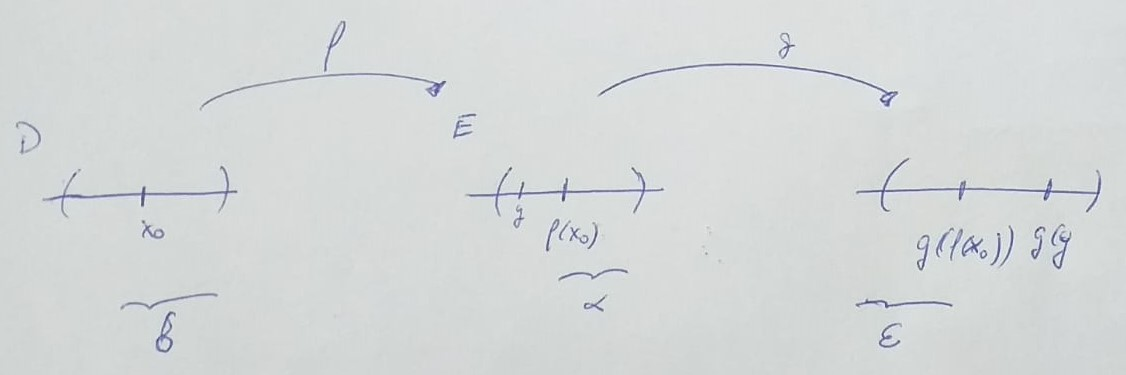
\includegraphics[scale=0.35]{continuidad de composicion}
\end{center}

Por lo que tenemos que:
$$x\in D \wedge |x-x_0|<\delta\Rightarrow |\underbrace{f(x)}_{\in E}-f(x_0)|<\alpha\Leftrightarrow |y-f(x_0)|<\alpha\Rightarrow |g(f(x))-g(f(x_0))|<\varepsilon$$

\item Es la demostración de 1. pero aplicada a todo $x_0\in D$, es decir, ocurre la 1. pero en todos los puntos de $D$. 

\item Podemos hacer la demostración del apartado 1 pero por sucesiones:
$$\mbox{Sea }\{x_n\}_{n=1}^\infty\subset D: x_n\xrightarrow{n\rightarrow\infty} x_0\stackrel{f \mbox{ cont.}}{\Rightarrow} f(x_n)\xrightarrow{n\rightarrow\infty} f(x_0)\stackrel{g \mbox{ cont.}}{\Rightarrow}g(f(x_n))\xrightarrow{n\rightarrow \infty} g(f(x_0))\Rightarrow$$
$$\Rightarrow g\circ f\mbox{ cont. en } x_0$$
\end{enumerate}
\end{demo}

\begin{prop}
Sea $I\subset \mathbb R$ un intervalo y $f: I\longrightarrow \mathbb R$ continua e inyectiva (entonces biyectiva sobre $f(I)$), entonces:
$$\exists f^{-1}: f(I)\longrightarrow I\mbox{ continua}$$
\end{prop}
\begin{demo}
\begin{itemize}
\item Supongamos primero que el intervalo es cerrado y acotado: $I=[a,b]$ y sea $y_0\in f(I)=D$, escogemos una sucesión convergente a un número de la imagen, entonces: sea $\{y_n\}_{n=1}^\infty \subset D: y_n\xrightarrow{n\rightarrow \infty} y_0$. Veamos que $f^{-1}(y_n)\xrightarrow{n\rightarrow\infty} f^{-1}(y_0)$:
$$\mbox{Sea }x_n=f^{-1}(y_n)\mbox{ y }x_0=f^{-1}(y_0)\Rightarrow \{x_n\}\subset I\mbox{ y }x_0\in I$$

Por el \textbf{Teorema de Bolzano-Wierstrass}, entonces $\{x_n\}$ tiene subsucesiones convergentes. Cojamos una cualquiera, sea $\{x_{n_k}\}_{k=1}^\infty$ una subsucesión que converge a $l\in [a,b]$, entonces $x_{n_k}\xrightarrow{k\rightarrow \infty }l\mbox{ y como f es continua, entonces } f(x_{n_k})\xrightarrow{k\rightarrow \infty}f(l)$, por lo tanto:
$$\underbrace{f(x_{n_k})}_{y_{n_k}}\xrightarrow{k\rightarrow \infty}f(l)\Leftrightarrow y_{n_k}\xrightarrow{k\rightarrow \infty}\underbrace{f(l)}_{y_0}\Rightarrow \underbrace{y_0}_{f(x_0)}=f(l)\Leftrightarrow y_0=f(x_0)=f(l)\stackrel{Biyec.}{\Rightarrow}x_0=l$$

Veamos que efectivamente $x_n\xrightarrow{n\rightarrow\infty}x_0$, hemos demostrado que cualquier subsucesión convergente de $\{x_n\}_{n=1}^\infty$ converge a $x_0$, pero no hemos demostrado que todas converjan. Supongamos que hay una que no converge:
$$\exists \delta>0 \wedge \exists \{x_{n_k}\}_{k=1}^\infty\subset I: |x_{n_k}-x_0|>\delta$$
Es decir, hay términos de la sucesión que no se acercan a $x_0$, pero como la subsucesión está acotada por pertenecer a $I$, entonces por el teorema de \textbf{Bolzano-Wierstrass} posee alguna subsucesión convergente y, por lo demostrado antes, esa subsucesión de la subsucesión converge a $x_0$:
$$\Rightarrow \{x_{n_k}\}_{k=1}^\infty\mbox{ posee subsucesion convergente}\Rightarrow \mbox{converge a }x_0\Rightarrow \#$$

Esto es cierto porque si la subsucesión convergente, aunque sea subsucesión de la subsucesión también lo es de la sucesión inicial, por lo que cumple lo demostrado antes para la subsucesiones convergentes. Además al probar esto, ese hecho contradice la premisa de no ser convergente a $x_0$

\item Si $I$ es un intervalo cualquiera, sea $y_0\in f(I)$ y sea $x_0=f^{-1}(y_0)$ podemos encontrar SIEMPRE $a,b\in \mathbb R: x_0\in [a,b]\in I$ y entonces podemos volver al caso anterior.
\end{itemize}
\end{demo}

\begin{defi}[Límites Laterales]
Sea $f: (a,b)\longrightarrow \mathbb R$, entonces:
\begin{enumerate}
\item Si $x_0\in (a,b]$, decimos que $l\in \mathbb R$ es el \textbf{límite por la izquierda de $f$ en $x_0$} si y sólo si:
$$\lim_{x\rightarrow x_0^-}f(x)=l\Leftrightarrow \forall \varepsilon>0, \exists \delta>0: x\in (x_0-\delta, x_0)\Rightarrow |f(x)-l|<\varepsilon$$

\item Si $x_0\in [a,b)$, decimos que $l\in \mathbb R$ es el \textbf{límite por la derecha de $f$ en $x_0$} si y sólo si:
$$\lim_{x\rightarrow x_0^+}f(x)=l\Leftrightarrow \forall \varepsilon>0, \exists \delta>0: x\in (x_0, x_0+\delta)\Rightarrow |f(x)-l|<\varepsilon$$
\end{enumerate}
\end{defi}

\begin{prop}
Sea $f: (a,b)\longrightarrow \mathbb R$, entonces:
\begin{enumerate}
\item $\lim_{x\rightarrow x_0^-}f(x)=l\Leftrightarrow \forall \{x_n\}_{n=1}^\infty \subset (a,b): x_n\xrightarrow{n\rightarrow \infty} x_0: x_n<x_0: \forall n\in \mathbb N\Rightarrow f(x_n)\xrightarrow{n\rightarrow \infty}l$

\item $\lim_{x\rightarrow x_0^+}f(x)=l\Leftrightarrow \forall \{x_n\}_{n=1}^\infty \subset (a,b): x_n\xrightarrow{n\rightarrow \infty} x_0: x_n>x_0: \forall n\in \mathbb N\Rightarrow f(x_n)\xrightarrow{n\rightarrow \infty}l$

\item $f(x_0^-)$ y $f(x_0^+)$ si existen son únicos.
\end{enumerate}
\end{prop}
\begin{demo}
\begin{enumerate}
\item 
	\begin{itemize}
	\item ``$\Rightarrow$'':\par
	Sea $\{x_n\}\subset (a,b):  x_n\xrightarrow{n\rightarrow \infty} x_0: x_n< x_0: \forall n\in \mathbb N$. Sabemos porque es límite que dado $\varepsilon>0, \exists \delta>0: x\in(x_0-\delta, x_0)\Rightarrow |f(x)-l|<\varepsilon$, pero como sabemos que la sucesión converge a $x_0$, entonces dado $\varepsilon>0, \exists n_0\in \mathbb N: \forall n\geq n_0: x_n\in (x_0-\delta, x_0)\Rightarrow |f(x_n)-l|<\varepsilon$
	
	\item ``$\Leftarrow$'':\par
	Si $l$ no es $f(x_0^-)\Rightarrow \exists \varepsilon>0:\forall \delta>0: \exists x\in(x_0-\delta, x_0): |f(x)-l|\geq \varepsilon$. Vamos a construir una sucesión que se acerca por la izquierda y cuyas imágenes no convergen a $l$ para todo $\varepsilon$.
	$$\delta=\frac{1}{n}: n\in \mathbb N \Rightarrow \forall \delta=\frac{1}{n} : \exists x_n\in \left(x_0-\frac{1}{n}, x_0\right): |f(x_n)-l|\geq \varepsilon $$
	
	Vemos que tenemos una sucesión de manera que $ x_n\xrightarrow{n\rightarrow \infty} x_0$ porque cuando $n\rightarrow \infty\Rightarrow |x_0-\frac{1}{n}|<\varepsilon$, es decir, cuanto más grande es $n$, más cerca del límite están los números de la sucesión, pero sus imágenes no convergen a $l$ por haberla escogido así: $f(x_n)\cancel{\xrightarrow{n\rightarrow \infty}}l$, luego \#.
	\end{itemize}
	
\item Análogo a la anterior

\item La misma demostración que para la unicidad del límite, se trata de coger un $\varepsilon$ de manera que los entornos de $l_1$ y $l_2$ sean disjuntos.

\begin{center}
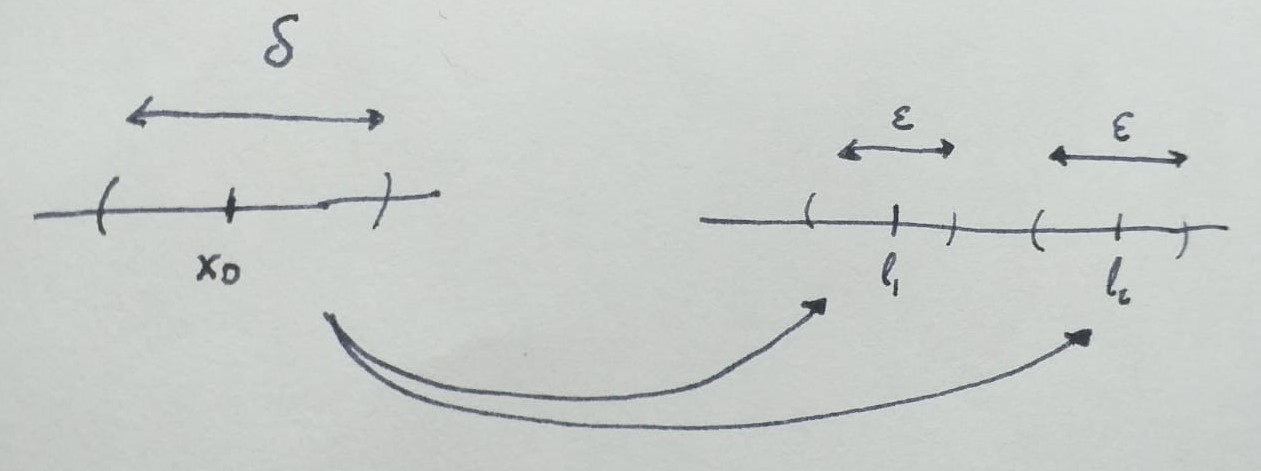
\includegraphics[scale=0.25]{unicidad limite lateral}
\end{center}

\end{enumerate}
\end{demo}

\begin{theo}[Caracterización de la continuidad]
Sea $f: (a,b)\longrightarrow \mathbb R$ y $x_0\in (a,b)$, entonces:
\begin{enumerate}
\item $\exists \lim_{x\rightarrow x_0} f(x)=l\Leftrightarrow f(x_0^-)=f(x_0^+)=l$

\item $f \mbox{ es continua en }x_0 \Leftrightarrow f(x_0^-)=f(x_0^+)=f(x_0)$
\end{enumerate}
\end{theo}
\begin{demo}
\begin{enumerate}
\item 
	\begin{itemize}
	\item ``$\Rightarrow $'':
	$$\forall\varepsilon>0: \exists \delta>0: x\in (x_0-\delta, x_0+\delta)\mbox{\textbackslash}\{x_0\}\Rightarrow |f(x)-l|<\varepsilon$$
	Y ya está porque si los números de ese intervalo lo cumplen, entonces los números del intervalo $(x_0-\delta, x_0)$ y $(x_0, x_0+\delta)$ también.
	
	\item ``$\Leftarrow$'':
	$$\forall \varepsilon>0\begin{cases}\exists \delta_1>0: x\in (x_0-\delta_1, x_0)\Rightarrow |f(x)-l|<\varepsilon \\
	\exists \delta_2>0: x\in (x_0,x_0+\delta_2)\Rightarrow |f(x)-l|<\varepsilon\end{cases}$$
	
 	Sea $\delta =min\{ \delta_1, \delta_2\}$, entonces:
	$$x\in (x_0-\delta, x_0+\delta)\mbox{\textbackslash}\{x_0\}\Rightarrow |f(x)-l|<\varepsilon$$
	\end{itemize}
	
\item Demostrado porque para ser continua el límite tiene que ser igual a $f(x_0)$ y para que exista el límite tiene que ser igual a él los límites laterales.
\end{enumerate}
\end{demo}

\begin{defi}[Discontinuidades]
Sea $f: (a,b)\longrightarrow \mathbb R$ y $x_0\in (a,b)$, si $f$ no es continua en $x_0$, entonces:
\begin{itemize}
\item Existen $f(x_0^+)$ y $f(x_0^-)$:
	\begin{itemize}
	\item \textbf{Discontinuidad evitable}: $f(x_0^-)=f(x_0^+)$, pero distintos a $f(x_0)$
	\item \textbf{Discontinuidad de salto}: $f(x_0^-)\neq f(x_0^+)$
		\begin{itemize}
		\item \textbf{Salto finito}: $f(x_0^-), f(x_0^+) < \infty$.
		\item \textbf{Salto infinito}: $f(x_0^-) > \pm\infty$ o $f(x_0^+) > \pm\infty$.
		\end{itemize}
	\end{itemize}
	
\item No existe alguno de los dos límites laterales:
	\begin{itemize}
	\item \textbf{Discontinuidad esencial}: $\nexists f(x_0^-)$ o $\nexists f(x_0^+)$
	\end{itemize}
\end{itemize}
\end{defi}

\begin{defi}[Límites Laterales en $\bar{\mathbb{R}}$]
Sea $f: (a,b)\longrightarrow \mathbb R$, entonces:
\begin{itemize}
\item Si $x_0\in (a,b]$, decimos que:
$$\lim_{x\rightarrow x_0^-}f(x)=\infty\Leftrightarrow \forall M>0: \exists \delta>0: x\in (x_0-\delta, x_0)\Rightarrow f(x)\geq M$$

\item Si $x_0\in (a,b]$, decimos que:
$$\lim_{x\rightarrow x_0^-}f(x)=-\infty\Leftrightarrow \forall M>0: \exists \delta>0: x\in (x_0-\delta, x_0)\Rightarrow f(x)< -M$$

\item Si $x_0\in [a,b)$, decimos que:
$$\lim_{x\rightarrow x_0^+}f(x)=\infty\Leftrightarrow \forall M>0: \exists \delta>0: x\in (x_0,x_0+\delta)\Rightarrow f(x)\geq M$$

\item Si $x_0\in [a,b)$, decimos que:
$$\lim_{x\rightarrow x_0^+}f(x)=-\infty\Leftrightarrow \forall M>0: \exists \delta>0: x\in (x_0,x_0+\delta)\Rightarrow f(x)< -M$$
\end{itemize}
\end{defi}

\begin{prop}
Sea $f: (a,b)\longrightarrow \mathbb R$, entonces:
\begin{itemize}
\item Si $x_0\in (a,b)$, decimos que:
$$\lim_{x\rightarrow x_0}f(x)=\infty\Leftrightarrow \lim_{x\rightarrow x_0^-}f(x)=\infty \wedge \lim_{x\rightarrow x_0^+}f(x)=\infty$$

\item Si $x_0\in (a,b)$, decimos que:
$$\lim_{x\rightarrow x_0}f(x)=-\infty\Leftrightarrow \lim_{x\rightarrow x_0^-}f(x)=-\infty \wedge \lim_{x\rightarrow x_0^+}f(x)=-\infty$$

\item Si $x_0\in (a,b]$, decimos que:
$$\lim_{x\rightarrow x_0^-}f(x)=\infty\Leftrightarrow \forall \{x_n\}_{n=1}^\infty \subset (a,b): x_n\xrightarrow{n\rightarrow\infty} x_0: x_n<x_0: \forall n\in \mathbb N\Rightarrow f(x_n)\xrightarrow{n\rightarrow \infty} \infty$$

\item Si $x_0\in (a,b]$, decimos que:
$$\lim_{x\rightarrow x_0^-}f(x)=-\infty\Leftrightarrow \forall \{x_n\}_{n=1}^\infty \subset (a,b): x_n\xrightarrow{n\rightarrow\infty} x_0: x_n<x_0: \forall n\in \mathbb N\Rightarrow f(x_n)\xrightarrow{n\rightarrow \infty} -\infty$$

\item Si $x_0\in [a,b)$, decimos que:
$$\lim_{x\rightarrow x_0^+}f(x)=\infty\Leftrightarrow \forall \{x_n\}_{n=1}^\infty \subset (a,b): x_n\xrightarrow{n\rightarrow\infty} x_0: x_n>x_0: \forall n\in \mathbb N\Rightarrow f(x_n)\xrightarrow{n\rightarrow \infty} \infty$$

\item Si $x_0\in [a,b)$, decimos que:
$$\lim_{x\rightarrow x_0^+}f(x)=-\infty\Leftrightarrow \forall \{x_n\}_{n=1}^\infty \subset (a,b): x_n\xrightarrow{n\rightarrow\infty} x_0: x_n>x_0: \forall n\in \mathbb N\Rightarrow f(x_n)\xrightarrow{n\rightarrow \infty} -\infty$$
\end{itemize}
\end{prop}

\subsection{Teoremas Fundamentales de Funciones Continuas}
\begin{theo}[de Wierstrass]
Sea $f:[a,b] \rightarrow \mathbb R$ continua, entonces:
\begin{itemize}
\item Es acotada: $\exists M>0: \forall x\in [a,b]: |f(x)|\leq M$

\item Se alcanzan el máximo y el mínimo: $\exists c,d\in [a,b]: \begin{cases} f(c)=\inf\{f(x): x\in [a,b]\} \\ f(d)=\sup\{f(x): x\in [a,b]\}\end{cases}$
\end{itemize}
\end{theo}
\begin{demo}
\begin{enumerate}
\item Supongamos que no es acotada superiormente (y el inferiormente es análogo):
$$\forall n\in \mathbb N: \exists x_n\in [a,b]: f(x_n)>n$$
Entonces tenemos que $\{x_n\}_{n\in \mathbb N}\subset [a,b]$ y por el teorema de Bolzano-Wiestrass: $\exists \{x_{n_k}\}$ convergente (a $x_0$) y como $f$ es continua entonces $f(x_n)$ converge a $f(x_0)$, por lo probado en teoremas anteriores, y teníamos que $f(x_{n_k})>n_k$ que converge a infinito, luego \#.

\item Como está acotado, su supremo existe: $S=\sup\{f(x): x\in [a,b]\}$ y su ínfimo $I=\inf\{f(x): x\in [a,b]\}$, entonces\footnote{Hacemos la del supremo porque la del ínfimo es análoga} como es supremo:
$$\forall n\in \mathbb N: \exists x_n\in [a,b]: S-\frac{1}{n}<f(x_n)\leq S$$
Esto forma una sucesión de números. Como sabemos que $\{x_n\}\subset[a,b]$, entonces por el Teorema de Bolzano-Wierstrass, tenemos que $\exists \{x_{n_k}\}$ que converge (a $d$) por lo que tenemos que $f(x_{n_k})$ converge a $f(d)$ y como $f(x_n)$ converge a $S$, entonces $f(d)=S$.
\end{enumerate}
\end{demo}

\begin{obs}
Se puede anotar como observación que cuando la función no es continua esto es falso y del mismo modo cuando el intervalo es abierto no ocurre.
$$f(x)=\begin{cases} \frac{1}{x} & \mbox{ si }x\neq 0 \\ 0 &\mbox{ si }x=0\end{cases} \mbox{ donde }x\in [-1,1]\Rightarrow \mbox{ no acotada}$$
$$f(x)=\begin{cases} \frac{1}{x} & \mbox{ si }x\neq 0 \\ 0 &\mbox{ si }x=0\end{cases} \mbox{ donde }x\in (0,1)\Rightarrow \mbox{ no alcanza su máximo y su mínimo}$$
\end{obs}

\begin{theo}[de Bolzano]
Sea $f:[a,b] \rightarrow \mathbb R$ continua tal que $f(a)<0$ y $f(b)>0$, entonces $\exists c\in (a,b): f(c)=0$.
\end{theo}
\begin{demo}
Supongamos que $f(a)<0$ y $f(b)>0$, entonces sea $A=\{t\in [a,b]: f(t)<0\}$ tenemos que $a\in A$ y $b$ es cota superior de $A$ y, en consecuencia, existe el supremo que llamaremos $\exists \sup(A)=c$. Entonces existe una sucesión de puntos de $A$ que converge a su supremo porque $\forall n\in \mathbb N: \exists t_n\in A: c-\frac{1}{n}< t_n\leq c$, es decir, $\exists\{t_n\}\subset A: t_n\xrightarrow{n\rightarrow \infty}c$. Como $f$ es continua, entonces $f(t_n)\xrightarrow{n\rightarrow \infty}f(c)\Rightarrow f(c)\leq 0)$ y ahora probamos que $f(c)=0$.\par
Si $f(c)<0\Rightarrow \exists\delta>0: \forall x\in (c-\delta, c+\delta): f(x)<0\Rightarrow (c-\delta, c+\delta)\subset A$, lo que contradice que $c=\sup A\Rightarrow \#\Rightarrow f(c)=0\Rightarrow c\in (a,b)$ porque $f(a)\neq 0$ y $f(b)\neq 0$.
\end{demo}

\begin{theo}[del valor intermedio]
Sea $f:[a,b] \rightarrow \mathbb R$ una función continua tal que\footnote{Para el enunciado del teorema se ha supuesto que $A < B$ pero es indiferente para el resultado.} $A=f(a)$ y $B=f(b)$, entonces:
$$\forall C \in (A,B) : \exists c \in (a,b) : f(c) = C$$
es decir, que una función continua alcanza todos los valores intermedios entre dos de sus imágenes.
\end{theo}
\begin{demo}
Llamamos $g(x)=f(x)-C$ de manera que $g:[a,b] \rightarrow \mathbb R$ y es continua. Es fácil ver que:
$$\begin{cases}g(a)=f(a)-C=A-C \\ 
g(b)=f(b)-C=B-C \end{cases} \Rightarrow \mbox{ signos distintos}\stackrel{Bolzano}{\Rightarrow} \exists c\in (a,b): g(c)=0$$
\end{demo}

\begin{prop}
Sea $f:[a,b] \rightarrow \mathbb R$ continua, entonces $f([a,b])$ es un intervalo cerrado y acotado, formado por el ínfimo y el supremo de las imágenes.
\end{prop}
\begin{demo}
Por el teorema de Wiestrass, hemos visto que:
$$\exists c,d\in [a,b]:\begin{cases}f(c)=\inf\{f(x): x\in [a,b]\} \\ f(d)=\sup \{f(x):x\in [a,b]\} \end{cases}$$
En particular, $\forall x\in [a,b]$ tenemos que:
$$f(c)\leq f(x)\leq f(d)\Rightarrow f([a,b])\subset [f(c), f(d)]$$
Veamos ahora $``\supset''$:\par
Sea $y\in [f(c), f(d)]$ suponiendo que es distinto de $f(c)$ y $f(d)$ como $f:[c,d]\rightarrow \mathbb R$ continua por el teorema de valores intermedios, entonces $\exists x\in [c,d]: f(x)=y\Rightarrow y\in f([c,d])\subset f([a,b])$.
\end{demo}

\begin{prop}
Sea $I\subset \mathbb R$ un intervalo, si $f: I\rightarrow |\mathbb R$ y es continua, entonces $f(I)$ es un intervalo.
\end{prop}
\begin{demo}
Sea $\alpha, \beta\in f(I)$, veamos que $[\alpha, \beta]\subset f(I)\Rightarrow f(I)$ es un intervalo:
Teniendo en cuenta lo primero podemos asegurar que $\exists a, b \in I: \alpha=f(a) \wedge \beta=f(b)$. Podemos suponer sin pérdida de generalidad que $a<b\Rightarrow [a,b]\subset I$ y como $f:[a,b]\rightarrow \mathbb R$ es continua, entonces si $y \in [\alpha,\beta]$ tenemos que $\exists c\in [a,b]\subset I: f(c)=y\in f(I)$.
\end{demo}

\subsubsection{Continuidad uniforme}
La definicion de continuidad vista es: supongamos que tenemos $f: D\rightarrow \mathbb R$ donde $D\subset \mathbb R$ de manera que $f$ es continua en $D$, es decir:
$$\forall x\in D: \forall \varepsilon>0: \exists \delta>0 : x,y \in D: |x-y|<\delta\Rightarrow |f(x)-f(y)|<\varepsilon$$
Esto quiere decir que una vez fijo el $x$, para cualquier $\varepsilon$ escogido, siempre podemos encontrar un $\delta$ de manera que se cumpla lo que sigue.

La aproximación que ofrecemos en este subapartado es completamente distinta: elegimos el $\varepsilon$ primero y encontramos un $\delta$ que nos vale para cualesquiera dos puntos que estén a dicha distancia.

\begin{defi}[Continuidad uniforme]
Sea $f:D\rightarrow \mathbb{R}$ una función, decimos que es \textbf{uniformemente continua en $D$} si y sólo si:
$$\forall \varepsilon>0: \exists \delta>0 : \forall x, y \in D: |x-y|<\delta \Rightarrow |f(x)-f(y)|<\varepsilon$$
\end{defi}

Se ve, por tanto, que ponemos de manifiesto que escogido un $\varepsilon$ cualquiera, siempre podemos encontrar un $\delta$ de manera que para todos los $x$ e $y$ que estén a distancia menor que $\delta$ sus imágenes están lo suficientemente cerca.

\begin{obs}
\begin{enumerate}
\item Si $f$ es uniformemente continua en D, también es continua en D.

\item  El recíproco es falso:
\end{enumerate}
\end{obs}

\begin{ej}
$f: \mathbb R \rightarrow \mathbb R: f(x)=x^2$ es continua pero no uniformemente continua. Esto es así porque sea $\varepsilon=1$, $\delta >0$ y $x,x+\delta$ entonces tenemos que: $|f(x)-f(x+\delta)|=|x^2|-(x+\delta)^2=\delta|\delta +2x|$. Si dado el delta yo escojo un $x$ de manera que $\delta +2x > \frac{1}{\delta}$, entonces $\delta|\delta +2x|>1$, por lo que no es uniformemente continua porque hemos encontrado un $x$ que no satisface la propiedad.
\end{ej}

\begin{theo}
Sea $f:[a,b]\rightarrow \mathbb R$ continua, entonces es uniformemente continua en un intervalo cerrado y acotado.
\end{theo}
\begin{demo}
Supongamos que $f$ no es uniformemente continua, entonces $\exists \varepsilon> 0: \forall \delta>0: \exists x,y\in [a,b]: |x-y|<\delta$ y $|f(x)-f(y)|\geq \varepsilon$. Para $\delta = \frac{1}{n}: n\in \mathbb N$, entonces $\exists x_n, y_n\in [a,b]: |x_n-y_n|<\frac{1}{n}$ y $|f(x_n)-f(y_n)|\geq \varepsilon$. Pero entonces tenemos $\{x_n\}\in [a,b]$ y por el teorema de Bolzano-Wierstrass, $\exists \{x_{n_k}\}$ subsucesión convergente a $l\in [a,b]$ de manera que $|x_{n_k}-y_{n_k}| < \frac{1}{n} \xrightarrow{n\rightarrow \infty} 0\Rightarrow |x_{n_k}-y_{n_k}|\xrightarrow{n\rightarrow \infty} 0\Rightarrow y_{n_k}=x_{n_k}+(y_{n_k}-x_{n_k})\stackrel{n\rightarrow \infty}{\Leftrightarrow} y_{n_k}\rightarrow l+0=l$

Pero por otro lado, las imágenes están lejos porque como f es continua, entonces $f(x_{n_k})\xrightarrow{k\rightarrow \infty}f(l)$ y $f(y_{n_k})\xrightarrow{k\rightarrow \infty}f(l)$, pero tenemos que $|f(x_{n_k})-f(y_{n_k})|\geq 0$ y es absurdo porque cuando se tiende a infinito tenemos que $|l-l|=0<\varepsilon\Rightarrow \#$.
\end{demo}

\subsection{Funciones Monótonas}
Cabe destacar y mencionar en este capítulo una serie de funciones muy relevantes: las funciones monótonas. Vamos a estudiar que propiedades ofrece la monotonía y por qué son tan importantes en el estudio del análisis de variable real. 

\begin{defi}[Función Monótona]
Sea $f:[a,b]\rightarrow \mathbb R$, decimos\footnote{Le añadimos el sobrenombre de \textbf{estricta} si la desigualdad es estricta} que es:
\begin{itemize}
\item \textbf{Monótona Creciente}: $\forall x,y\in [a,b]: x<y\Rightarrow f(x)\leq f(y)$
\item \textbf{Monótona Decreciente}: $\forall x,y\in [a,b]: x<y\Rightarrow f(x)\geq f(y)$
\end{itemize}
\end{defi}

\begin{theo}
Sea $f:[a,b]\rightarrow \mathbb R$ monótona creciente\footnote{Con las decrecientes ocurre de forma análoga.}, entonces:
\begin{itemize}
\item $\forall x\in (a,b):\exists f(x^-)\mbox{ y }f(x^+): f(x^-)\leq f(x)\leq f(x^+)$
\item $\begin{cases}f(x^-)=\sup\{f(t): t<x\} \\ f(x^+)=\inf\{f(t): t>x\}\end{cases}$
\item $\forall x,y\in (a,b): x<y\Rightarrow f(x^+)\leq f(y^-)$
\end{itemize}
\end{theo}
\begin{demo}
Sea $x\in (a,b)$, $A_x=\{f(t): t<x\}$ y $B_x=\{f(t): t>x\}$ donde $t\in [a,b]$. Como $f$ es monótona creciente:
$$\begin{cases}\mbox{Si }t< x & f(t)\leq f(x)\Rightarrow f(x)\mbox{ es cota superior de }A_x \\\mbox{Si } x<t & f(x)\leq f(t)\Rightarrow f(x)\mbox{ es cota inferior de }B_x\end{cases}\Rightarrow \exists \xi=\sup A_x\mbox{ y }\exists \eta=\inf B_x$$
Veamos ahora que $\xi=f(x^-)$:
$$\mbox{Sea }\varepsilon>0\Rightarrow \exists t_1<x: \xi-\varepsilon< f(t_1)\leq \xi$$
Pero como la función es monótona creciente entonces si escogemos un $t$, de manera que $t_1<t<x\Rightarrow \xi- \varepsilon<f(t_1)<f(t)<\xi$.

En síntonía con lo anterior, sea $\delta= x-t_1>0$ tenemos que si $t\in (x-\delta, x)\Rightarrow f(t)\in (\xi-\varepsilon, \xi)\subset (\xi-\varepsilon, \xi+ \varepsilon)$ que es precisamente la definición de límite por la izquierda, con lo que queda probado que  $\xi=f(x^-)$.

Ahora probamos que $\eta=f(x^+)$:
$$\mbox{Sea }\varepsilon>0\Rightarrow \exists t_2>x: \eta< f(t_2)\leq \eta+ \varepsilon$$
Del mismo modo, sea $\delta= t_2-x$, si escogemos un $t$ de manera que $x<t<t_2\Rightarrow \eta\leq f(t)\leq f(t_2)<\eta+ \varepsilon \Rightarrow t\in (x, x+\delta)\Rightarrow f(t)\in (\eta, \eta+\varepsilon)\subset (\eta-\varepsilon, \eta+ \varepsilon)$ que es precisamente la definición de límite por la derecha, con lo que queda probado que  $\eta=f(x^+)$.

Si $x<y$, entonces sea $t: x<t<y$. Sabemos que $f(x^+)\leq f(t)$ y como también $f(t)\leq f(y^-)$, entonces tenemos que $f(x^+)\leq f(t)\leq f(y^-)$.
\end{demo}

\begin{obs}
El teorema se mantiene en $x=a$ y $x=b$ contando con que no existe el límite por la izquierda y por la derecha respectivamente. En consecuencia, podemos decir que las funciones monótonas solo tienen discontinuidades de salto.
\end{obs}

\begin{theo}
Sea $f:[a,b]\rightarrow \mathbb R$ monótona, entonces el conjunto de discontinuidades es, a lo sumo, \textbf{numerable}.
\end{theo}
\begin{demo}
Supongamos que $f$ es creciente\footnote{Con las decrecientes pasa lo mismo}. Llamamos $D=\{x\in (a,b): f \mbox{ es discontinua}\}$, sabemos también que $f$ es discontinua $\Leftrightarrow f(x^-)< f(x^+)$, entonces $\forall x \in D: \exists q_x\in \mathbb Q: f(x^-)<q_x<f(x^+)$. Entonces tenemos $s:D \rightarrow \mathbb Q$ donde a cada $x\rightarrow q_x$. Veamos que esta aplicación es inyectiva, por que sabemos que una función es siempre suprayectiva sobre su imagen y demostrar la inyectividad supone poder establecer una biyección con los naturales. Si $x_1<x_2\Rightarrow s(x_1)=q_{x_1}<f(x_1^+)\leq f(x_2^-)< q_{x_2}=s(x_2)$, por lo que es numerable.
\end{demo}

\begin{prop}
Sea $f:[a,b]\rightarrow \mathbb R$ continua, entonces:
\begin{enumerate}
\item $f$ es inyectiva si y sólo si $f$ es estrictamente monótona.
\item $f^{-1}: f([a,b])\rightarrow [a,b]$ es continua, estrictamente monótona y biyectiva si $f$ es inyectiva.
\end{enumerate}
\end{prop}
\begin{demo}
\begin{enumerate}
\item Vemos la doble implicación:
	\begin{itemize}
	\item ``$\Leftarrow$'':
	$$\forall x_1, x_2\in [a,b]: x_1<x_2\Rightarrow f(x_1)<f(x_2) \vee f(x_1)>f(x_2)\Rightarrow f(x_1)\neq f(x_2) \Rightarrow f\mbox{ inyectiva}$$
	
	\item ``$\Rightarrow$'':
	Sea $f$ continua e inyectiva, como $f([a,b])=[f(c), f(d)]$ donde $f(c)=\inf\{f(t): t\in [a,b]\}$ y $f(d)=\sup\{f(t): t\in [a,b]\}$. Además como $f$ es inyectiva, $f(c)\neq f(d)$ porque si fuese iguales la función sería constante lo cual es absurdo, esto implica que $f(c)<f(d)\Rightarrow c\neq d$.
	
	Supongamos que $c<d$, vamos a ver que necesariamente $c=a$, $d=b$ y que $f$ es estrictamente creciente.
	\begin{center}
	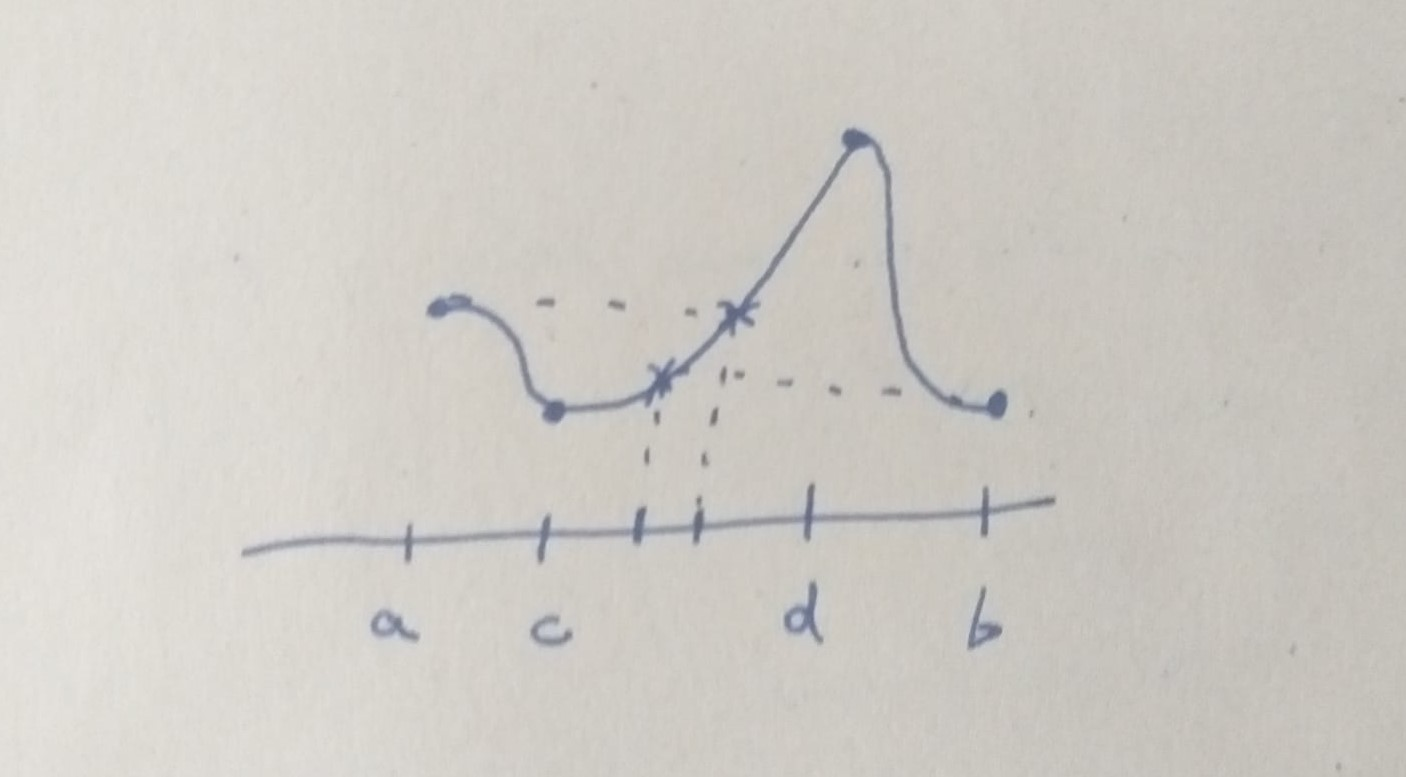
\includegraphics[scale=0.20]{inyectivas continuas son monotonas}
	\end{center}
	Supongamos que no, es decir, $a<c\Rightarrow f(c)< f(a)< f(d)$. Por el teorema de valores intermedios algún punto entre c y d tomará el valor de $f(a)$, por lo que $\exists t\in (c,d): f(t)=f(a)\Rightarrow $ no es inyectiva luego \#.
	
	Supongamos que $d<b$, vamos a ver que necesariamente $d=b$ y que $f$ es estrictamente creciente. Supongamos que no, es decir, $d<b\Rightarrow f(c)< f(b)< f(d)$. Por el teorema de valores intermedios algún punto entre c y d tomará el valor de f(b), con lo cual $\exists t\in (a,b): f(t)=f(b)\Rightarrow \#$ porque la hipótesis es que era inyectiva. Por lo que $a=c$ y $d=b$.
	
	\begin{center}
	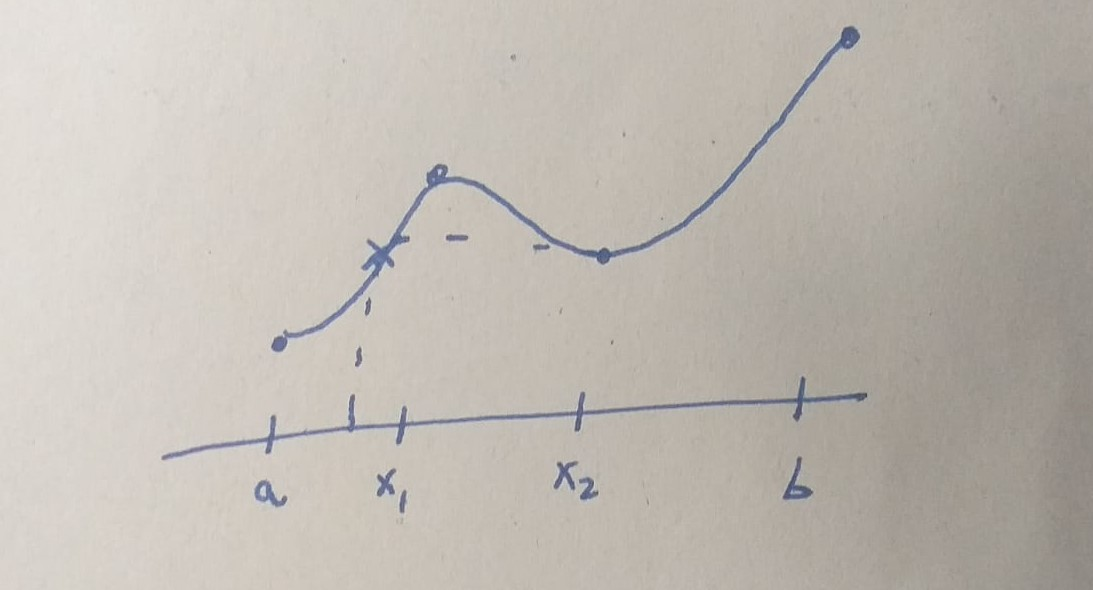
\includegraphics[scale=0.25]{inyectividad a monotonia en continuas1}
	\end{center}
	
	Con lo cual y viendo el dibujo, sabiendo que $a=c$ y que $b=d$, entonces veamos que es estrictamente creciente: supongamos que no $a\leq x_1< x_2 \leq b$ y $f(x_1)>f(x_2)\Rightarrow x_1\neq a$ porque es el ínfimo de las imágenes y además también $x_2\neq b$ por el mismo motivo. Con lo cual, $f(a)< f(x_2)< f(x_1)$. En consecuencia, por el teorema de valores intermedios en $[a,x_1]: \exists t\in (a,x_1): f(t)=f(x_2)\Rightarrow \#$ porque es inyectiva, con lo cual: $f(x_1)<f(x_2)$ y es estricta la desigualdad porque si fuese igual, no se cumpliría la inyectividad.\par
		
	Si tenemos el otro caso, en el que $c>d$, vamos a probar que $a=d$ y $c=b$ y que $f$ es estrictamente decreciente. Si $a<d$, entonces $f(c)<f(a)<f(d)$, entonces por el teorema de valores intermedios $\exists t\in (d,c): f(t)=f(a)\Rightarrow \#$. Si $c<b$, entonces de la misma manera ocurre por el teorema de valores intermedios que $f(c)< f(b)< f(d)\Rightarrow \exists t\in (c,d): f(t)=f(b)\Rightarrow \#$.\par

Con lo cual, sabiendo que $a=d$ y que $b=c$, entonces veamos que es estrictamente decreciente: supongamos que no $a\leq x_1< x_2 \leq b$ y $f(x_1)<f(x_2)\Rightarrow x_1\neq a$ porque es el supremo de las imágenes y además también $x_2\neq b$ por el mismo motivo. Con lo cual, $f(b)< f(x_1)< f(x_2)$. En consecuencia, por el teorema de valores intermedios en $[x_2,b]: \exists t\in (x_2,b): f(t)=f(x_1)\Rightarrow \#$ porque es inyectiva, con lo cual: $f(x_1)>f(x_2)$ y es estricta la desigualdad porque si fuese igual, no se cumpliría la inyectividad.\par
	\end{itemize}
	
\item Como lo anterior ya está demostrado, solo falta demostrar que la inversa también es estrictamente monótona. Sabemos que $f: [a,b]\rightarrow \mathbb R$ es estrictamente monótona. Ahora para hacer un caso\footnote{El caso decreciente es análogo} suponemos que $f$ es estrictamente creciente. Si $x_1,x_2\in [a,b]: x_1<x_2\Rightarrow f(x_1)<f(x_2)$, si $y_1,y_2\in f([a,b])=[f(c), f(d)]$ y además $y_1<y_2$, entonces sabemos por ser inyectiva que $\exists! x_1, x_2\in [a,b]: f(x_1)=y_1 < f(x_2)=y_2\Rightarrow x_1< x_2$ porque si fuese $x_1>x_2\Rightarrow f^{-1}(y_1)<f^{-1}(y_2)\Rightarrow f^{-1}$ es estrictamente creciente.
\end{enumerate} 
\end{demo}

\subsection{Continuidad de funciones elementales}
Como hemos visto que la suma, el producto y la composición de funciones continuas respeta la continuidad, si tenemos un buen alijo de funciones simples que se haya demostrado que sean continuas tendremos entonces una herramienta muy potente para demostrar que cualquier función lo es. Bastará con descomponerla en otras más pequeñas relacionadas entre sí por operaciones que respeten la continuidad.

\begin{theo}[Regla del Sandwich para funciones]
Sea $D\subset \mathbb R$, $x_0\in D'$ y $f,g,h: D\rightarrow\mathbb R$ dos funciones que verifican que :
\begin{itemize}
\item $\forall delta_0>0 : f(x)\leq g(x)\leq h(x)$
\item $\lim_{x\rightarrow x_0} f(x)=m$
\item $\lim_{x\rightarrow x_0} h(x) = m$
\end{itemize}
entonces se tiene que:
$$\overbrace{f(x)}^{\xrightarrow{x\rightarrow x_0} m} \leq g(x)\leq \overbrace{h(x)}^{\xrightarrow{x\rightarrow x_0}m}\Rightarrow g(x)\xrightarrow{x\rightarrow x_0}m$$
\end{theo}
\begin{demo}
Considerando que ambas funciones ``tapa'' tienden a $m$ tenemos que:
$$\forall \varepsilon>0 : \exists \delta_1>0 : 0<|x-x_0|<\delta_1\Rightarrow |f(x)-m|<\varepsilon$$
$$\forall \varepsilon>0: \exists \delta_2>0: 0<|x-x_0|<\delta_2\Rightarrow |h(x)-m|<\varepsilon$$
Luego si dado un $\varepsilon>0$, cogemos $\delta=\min\{\delta_0, \delta_1,\delta_2\}$ tenemos que:
$$m-\varepsilon< f(x) \leq g(x) \leq h(x) < m+\varepsilon\Rightarrow |g(x)-m|<\varepsilon$$
\end{demo}

\begin{theo}[Continuidad de la exponencial]
Sean $f: D\rightarrow (0,\infty)$ y $g: D\rightarrow \mathbb R$, entonces la función:
\begin{eqnarray*}
h: D &\longrightarrow \mathbb R \\
x &\longmapsto f(x)^{g(x)}
\end{eqnarray*}
es una función continua. 
\end{theo}
\begin{demo}
Para demostrar esta proposición vamos a demostrar pequeños resultados intermedios:
$$f(x)=a^x \mbox{ es continua} \Leftrightarrow \forall\{x_n\}_{n=1}^\infty\subset D: x_n\xrightarrow{n\rightarrow\infty} x\Rightarrow f(x_n)\xrightarrow{n\rightarrow} f(x)$$
Como vimos en el tema de sucesiones, el límite se puede pasar al exponente así que se tiene que: $f(x_n)=a^x_n\xrightarrow{n\rightarrow\infty} a^x\Rightarrow f$ es continua. Por el teorema que dice que la composición de funciones continuas es continua, se tiene que: $f(x)=a^{g(x)}$ es continua.

Del mismo modo, tenemos que $f(x)=x^a$ es continua porque por el mismo razonamiento: $f(x_n)=x_n^a\xrightarrow{n\rightarrow\infty} x^a$, luego se cumple. En consecuencia, tenemos que por la composición: $f(x)=g(x)^a$ es continua.

Basta con ver que al ser estas dos funciones continuas, la composición de ambas: $h(x)=f(x)^{g(x)}$ es continua.
\end{demo}

\begin{theo}
La funciones trigonométricas seno y coseno, es decir, $\sin x$ y $\cos x$ son funciones continuas.
\end{theo}

\begin{theo}[Continuidad del logaritmo]
Sea $a\in \mathbb{R}$ un número positivo, definimos el \textbf{logaritmo en base $a$} como la función inversa a la exponencial, es decir:
\begin{eqnarray*} log_a x: (0,\infty) &\longrightarrow& \mathbb R \\ a^x &\longmapsto& x \end{eqnarray*}
Además observamos las siguientes propiedades:
\begin{itemize}
\item $\log_a xy = \log_a x + \log_a y$
\item $\log_a \frac{x}{y} = \log_a x - \log_a y$
\item $\log_a x^b = b\cdot \log_a x$
\item $\log_a x = \frac{\ln x}{\ln a}$
\item $\log_a a = 1$
\item $\log_a 0 \rightarrow -\infty$
\end{itemize}
\end{theo}
\begin{demo}
Como ya demostramos que $f(x)=a^x$, era continua, monótona e inyectiva y también estaba demostrado que toda función es sobreyectiva sobre su imagen, vemos que la inversa existe: a esta es a la que denominamos \textit{logaritmo}. Veamos que su dominio es $(0,\infty)$:\par
Si $a>1$, entonces $\lim_n\rightarrow \infty a^n = \infty$ y $\lim_n\rightarrow \infty a^-n = 0$, por lo que la imagen siempre es positiva. Como $\mathbb R$ es un intervalo, sabemos que la imagen de un intervalo por una función continua es de nuevo un intervalo lo que implica que $f(\mathbb R)\subset (0,\infty)$ y como las imágenes de antes tendían a 0 y a $\infty$ necesariamente la imagen es $(0,\infty)$. El caso de que $0<a<1$ es análogo. En consecuencia, imagen de $a^x$ es el dominio de la función inversa.

Para las propiedades, tal y como hemos definido el logaritmo este representa el exponente al que debe elevarse la base para que pueda ser x, con lo cual $a^{\log_a x} = x$ así que:
$$a^{\log_a xy}= xy=a^{log_a x}\cdot a^{log_a y}=a^{\log_a x + \log_a y}\Rightarrow \log_a xy = \log_a x +\log_a y$$
El resto de propiedades se demuestran de forma análoga.
\end{demo}

\chapter{Cálculo Diferencial}
En este capítulo desarrollamos otro de los temas centrales del cálculo y el análisis matemático: la derivación. El problema surge del estudio de cambios en el valor de la función ante cambios infinitesimales de la entrada de la misma. Además, dicho concepto se relaciona íntimamente con las curvas y rectas tangentes a distintas superficies y con la optimización de funciones a través de máximos y mínimos.

\section{Derivabilidad}
En esta primera parte vamos a desarrollar toda la teoría necesaria para comprender el concepto de derivada, saber cómo operar con él y qué propiedades tiene para luego poder aplicar los resultados de forma eficiente.

\subsection{Concepto de Derivada}
El objetivo principal es ver cómo se comporta el cociente $\frac{f(x) - f(c)}{x-c}$ cuando $x$ es muy próximo a $c$. Es decir, dado un punto $c$ cualquiera, queremos cuantificar cuánto varía la imagen por $f$ con respecto a la que nos da $f(c)$ cuando los puntos que observamos están a una distancia infinitesimal.

\begin{defi}[Derivabilidad]
Sea $f: I\rightarrow \mathbb R$ una función donde $I$ es un intervalo y $c\in I$, decimos que es \textbf{derivable o diferenciable en $c$} si y sólo si $\exists L\in \mathbb R$ que verifica:
$$\forall \varepsilon>0: \exists \delta>0 : 0<|x-c|<\delta\Rightarrow \left|\frac{f(x)-f(c)}{x-c}-L\right|<\varepsilon$$
En este caso\footnote{Cabe destacar que $c$ puede ser un extremo del intervalo y que además $c$ debe pertenecer al dominio porque debemos poder calcular $f(c)$.} decimos que $L$ es la derivada de $f$ en $c$ y escribimos $f'(c)=L$.
\end{defi}

\begin{obs}
Esta definición es equivalente a la siguiente: si definimos la función $\varphi(x) = \frac{f(x)-f(c)}{x-c}$ donde $x\in I\mbox{\textbackslash}\{c\}$ entonces podemos redefinir la derivada como:
$$f\mbox{ es derivable en }c\Leftrightarrow \exists \lim_{x\rightarrow c}\varphi(x) = L$$
Esta caracterización es importante porque hemos visto y trabajado la demostración de la existencia o no de un límite y el cálculo de los mismos, por lo que en ocasiones puede facilitarnos el trabajo usar esta alternativa en vez de la definición.
\end{obs}

\begin{ej}
Sea $f: \mathbb R \rightarrow \mathbb R: f(x)=x^2$, luego hay que estudiar $\frac{f(x)-f(c)}{x-c} = \frac{x^2- c^2}{x-c}= x+c$, luego tenemos que $\lim_{x\rightarrow c} \frac{f(x)-f(c)}{x-c}= 2c$.\par
Veamos el mismo ejemplo con la definición, nuestro candidato es $f'(c)=2c$, la pregunta es si dado $\varepsilon>0$, puedo encontrar un $\delta$ de manera que se cumpla al definición?, veamos:
$$\left|\frac{f(x)-f(c)}{x-c}-2c\right| = \left|\frac{x^2-c^2}{x-c}-2c\right| = |x+c-2c|= |x-c|<\delta \Rightarrow \delta <\varepsilon$$
Luego bastaría con escoger un delta de manera que este sea menor que el epsilon dado.
\end{ej}

\begin{prop}
Si $f$ es derivable en $c$, entonces la derivada es única.
\end{prop}
\begin{demo}
$f$ es derivable en $c$ si y sólo si $\lim_{x\rightarrow c}\varphi(x) $ y como el límite es único, en consecuencia, la derivada debe ser un único valor.
\end{demo}

\begin{defi}[Función Derivada]
Sea $f:I\rightarrow \mathbb R$ derivable en todo $I$, definimos la \textbf{función derivada} como:
\begin{align*}
f': I &\rightarrow \mathbb R \\ c &\rightarrow f'(c)
\end{align*}
\end{defi}

\begin{ej}
Sea $f: \mathbb R \rightarrow \mathbb R: f(x)=x^2\Rightarrow f'(x)=2x$ como hemos visto antes.
\end{ej}

\begin{theo}
Si $f$ es derivable en $c$, entonces $f$ es continua en $c$.
\end{theo}
\begin{demo}
Sea $f:I\rightarrow \mathbb R$, $c\in I$, $\lim_{x\rightarrow c} \frac{f(x)-f(c)}{x-c}=f'(c)\in \mathbb R$, vemos que si $x\neq c$, entonces $f(x)-f(c)=\frac{f(x)-f(c)}{x-c} \cdot (x-c)$, pero sabemos que $\lim_{x\rightarrow c} \frac{f(x)-f(c)}{x-c} = f'(c)$ y que además $\lim_{x\rightarrow c} x-c =0$. Esto implica que
$$\exists \lim_{x\rightarrow c} (f(x)-f(c)) = \lim_{x\rightarrow c}\frac{f(x)-f(c)}{x-c} \cdot \lim_{x\rightarrow c}(x-c)= f'(c)\cdot 0 = 0 \Leftrightarrow \lim_{x\rightarrow c} f(x)= f(c)\Rightarrow f(x)\mbox{ continua en }c$$
\end{demo}

\begin{obs}
Sin embargo, en general el recíproco no es cierto, es decir, existe funciones continuas que no son derivables en algún punto de su dominio.
\end{obs}

\begin{ej}
Sea $f(x)=|x|$ tenemos que $f$ es continua en $x=0$ porque es continua en $\mathbb R$. Veamos que no es derivable en 0 ¿$\exists \lim_{x\rightarrow 0} \frac{f(x)-f(0)}{x-0}= \lim_{x\rightarrow 0}\frac{|x|}{x}$?:
$$\lim_{x\rightarrow 0^+} \frac{|x|}{x}=1$$
$$\lim_{x\rightarrow 0^-} \frac{|x|}{x}=-1$$
Luego no es derivable
\end{ej}

\subsubsection{Interpretación geométrica de la derivada}
Sea $f:I \rightarrow \mathbb R$ una función real y $c,a\in I$ puntos de su dominio, vamos a estudiar el valor de la pendiente\footnote{A pesar de darse esta explicación geométrica, en ningún caso intervendrá en cualesquiera de las demostraciones posteriores puesto que prevalece la definición de derivada dada} de la recta que pasa por $(cf,(c))$ y $(a,f(a))$.
$$m = \frac{f(a)-f(c)}{a-c}$$
Pero nos preguntamos ¿qué cambios sufrirá dicho valor si variamos el punto $a$?. Para ello, vamos a tomar $a$, como una variable, es decir, $x$, quedando el valor anterior como:
$$m = \frac{f(x)-f(c)}{x-c}$$
De este modo, para cada valor de $x$ tendremos el valor de la pendiente de la recta que une ambos puntos y ahora nos surge otra nueva pregunta: ¿qué pasará si escojo valores de $x$ cada vez más cercanos a $c$ o, lo que es lo mismo, si $x\rightarrow c$? La respuesta visualmente es sencilla:

\begin{center}
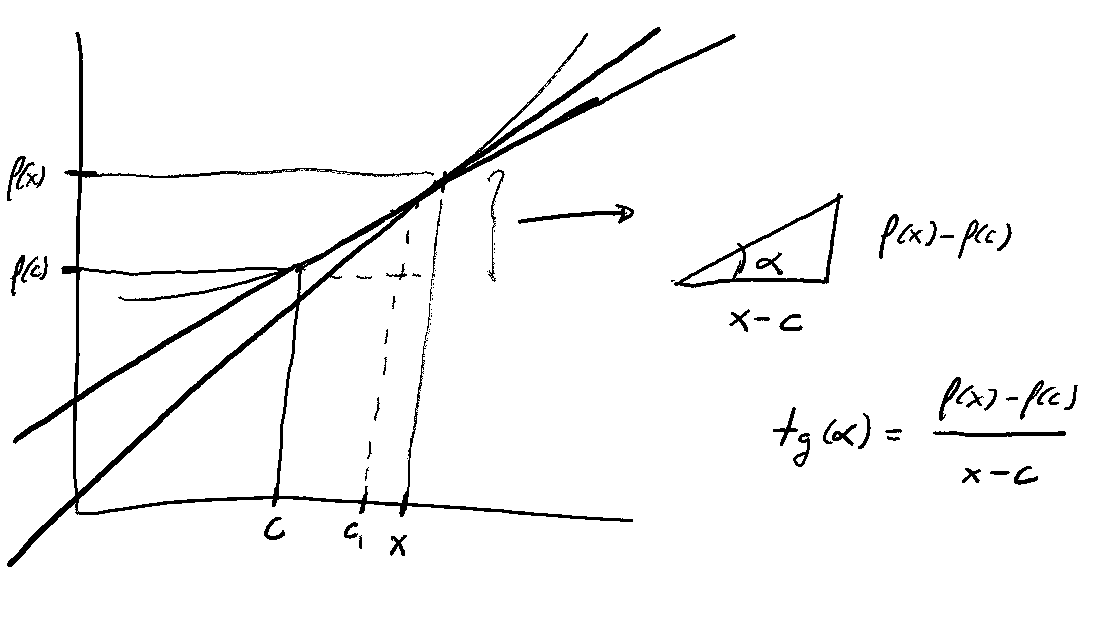
\includegraphics[scale=0.64]{Interpretacion derivada}
\end{center}

La recta, como pasa cada vez por dos puntos que están más próximos, tiene una pendiente más ajustada a la curva por el punto $c$. Cuando pasamos al límite, estamos diciendo que estamos ``tomando $x=c$'' y, en consecuencia, tenemos una recta tangente a $c$ en ese punto.

\subsection{Criterios de Derivabilidad}
Una vez definido y estudiado el concepto de derivada, es necesario entender cómo se relaciona este nuevo elemento matemático con las operaciones habituales de funciones sobre todo para saber en qué casos se conserva.

\begin{theo}[Operaciones con Derivabilidad]
Sean $f,g: I\rightarrow \mathbb R$ derivables en $c\in I$, se tiene que:
\begin{enumerate}
\item La función $f+g: I\rightarrow \mathbb R$ es derivable en $c$ y:
$$(f+g)'(c)=f'(c)+g'(c)$$
\item La función\footnote{$\alpha \in \mathbb R$} $\alpha \cdot f: I\rightarrow \mathbb R$ es derivable en $c$ y:
$$(\alpha \cdot f)'(c)=\alpha \cdot f'(c)$$
\item La función $f\cdot g: I\rightarrow \mathbb R$ es derivable en $c$ y:
$$(f\cdot g)'(c)=f'(c)g(c)+ f(c)g'(c)$$
\item La función\footnote{$g(c) \neq 0$} $\frac{f}{g}: I\rightarrow \mathbb R$ es derivable en $c$ y:
$$\left(\frac{f(c)}{g(c)}\right)'(c)=\frac{f'(c)g(c)-f(c)g'(c)}{g(c)^2}$$
\end{enumerate}
\end{theo}
\begin{demo}
Los dos primeros aparatados son muy sencillos.

3.

$$\lim_{x\rightarrow c}\frac{f(x)g(x)-f(c)g(c)}{x-c} = \lim_{x\rightarrow c} \frac{(f(x)-f(c))g(c)+f(c)g(x)-f(c)g(c)}{x-c}=$$
$$= \lim_{x\rightarrow c} \frac{(f(x)-f(c))g(c)+f(c)(g(x)-g(c))}{x-c} = \lim_{x\rightarrow c} \frac{f(x)-f(c)}{x-c}g(c)+f(c)\frac{g(x)-g(c)}{x-c}=$$
$$=f'(c)g(c)+f(c)g'(c)$$

4. Completamente análoga utilizando el truco usado en la 3.
\end{demo}

\begin{coro}
Sean $f_1, f_2, ..., f_n: I \rightarrow \mathbb R$ funciones derivables en $c\in I$, entonces:
\begin{enumerate}
\item $(f_1+...+f_n)'(c)=f_1'(c)+...+f'_n(c)$
\item $(f_1\cdot ... \cdot f_n)'(c)= f'_1(c)f_2(c)\cdot ... \cdot f_n(c)+ ... + f_1(c)\cdot ... \cdot f_{n-1}(c) \cdot f_n'(c)$
\end{enumerate}
\end{coro}
\begin{demo}
1. Trivial por la demostración de la suma simple

2. Supongamos cierta la proposición para $n$, lo demostramos para $n+1$:
$$(f_1 \cdot f_2 \cdot ... \cdot f_n \cdot f_{n+1})'=(g\cdot f_{n+1})'= g'(c)f_{n+1}(c)+ g(c)f_{n+1}'(c) =$$
$$= \left(f_1'(c)\cdot f_2(c) \cdot ... \cdot f_n(c) +...+ f_1(c)\cdot f_2(c)\cdot ...\cdot f'_n(c)\right)f_{n+1}(c)+(f_1(c)\cdot ...\cdot f_n(c))f_{n+1}'= $$
$$=f_1'(c)\cdot f_2(c) \cdot ... \cdot f_n(c)\cdot f_{n+1}(c) +...+ f_1(c)\cdot f_2(c)\cdot ...\cdot f'_n(c)f_{n+1}(c)+f_1(c)\cdot ...\cdot f_n(c)f_{n+1}'$$
\end{demo}

\begin{ej}
Si tenemos $f(x)=x^n= x\cdot x\cdots x$, entonces tenemos que por el corolario tenemos que: $f'(x)=1\cdot x \cdot ... \cdot x + ... + x\cdot ... \cdot x \cdot 1 = \underbrace{x^{n-1} + x^{n-1}+ ... + x^{n-1}}_{n \mbox{ veces}}= n\cdot x^{n-1}$

Con lo cual, podemos verlo en un caso general diciendo que $g(x)= f(x)^n$, por lo que $g'(c)= n\cdot f'(c)\cdot f(c)^{n-1}$.
\end{ej}

\begin{lema}[de Caratheodery]
Sea $f:I \rightarrow \mathbb R$, es derivable en $c\in I$ si y sólo si $\exists\varphi: I\rightarrow \mathbb R$ continua en $c$ de manera que $f(x)-f(c)=\varphi(x)(x-c): \forall x \in I$ de forma que $f'(c)=\varphi(c)$.
\end{lema}
\begin{demo}
\begin{itemize}
\item $\Rightarrow$:

Si $f$ es derivable en $c$, entonces $\varphi=\begin{cases} \frac{f(x)-f(c)}{x-c} & x\neq c \\ f'(c) & x=c\end{cases}$. Vemos que $\varphi$ es continua en $c$ puesto que $\lim_{x\rightarrow c}\varphi(x) = \lim_{x\rightarrow c} \frac{f(x)-f(c)}{x-c}=f'(c)=\varphi(c)$. Además se tiene que $f(x)-f(c)=\varphi(x)(x-c)$ cuando $x\neq c$, pero vemos que si $x=c$, entonces $f(x)-f(c)=\varphi(x)(x-c)\Leftrightarrow 0=\varphi(x)\cdot 0$, luego ocurre siempre.

\item $\Leftarrow$:

Si tenemos que $\varphi: I \rightarrow \mathbb R$ continua en c y $f(x)-f(c)=\varphi(x)(x-c) : x\in I$, entonces $x\neq c\Rightarrow \frac{f(x)-f(c)}{x-c}=\varphi(x)$ y como $\lim_{x\rightarrow c}\frac{f(x)-f(c)}{x-c} = \lim_{x\rightarrow c} \varphi(x)=\varphi(c)$, como el límite existe entonces f es derivable en c y $f'(c)=\varphi(c)$.
\end{itemize}
\end{demo}

\begin{theo}[Regla de la Cadena]
Sea $f: I \rightarrow \mathbb R $ derivable en $c\in I$, siendo $f(I)\subset J$ y $g: J\rightarrow \mathbb R$ una función derivable en $d=f(c)\in J$, entonces $g\circ f (x)$ es derivable en $c$ y:
$$(g\circ f)'(c)=g'(f(c))\cdot f'(c)$$
\end{theo}
\begin{demo}
Por el lema que acabamos de probar $f: I\rightarrow \mathbb R$ es derivable en $c$ si existe una función $\varphi: I\rightarrow \mathbb R$ continua en $c$ y se verifica que $f(x)-f(c)=\varphi(x)(x-c): x\in I$ y del mismo modo $g: I\rightarrow \mathbb R$ es derivable en $d$ si existe una función $\psi: J\rightarrow \mathbb R$ continua en $d$ de manera que se cumple que $g(z)-g(d)=\psi(z)(z-d): z\in J$.

En particular, si $z= f(x): x\in I$, entonces podemos decir que
$$g(f(x))-g(d)=\psi(f(x))(f(x)-\underbrace{d}_{f(c)})$$
Pero aplicando la otra condición tenemos que:
$$g(f(x))-g(d)=\psi(f(x))\varphi(x)(x-c)$$
Por tanto, si llamamos $\chi(x)= \psi((f(x))\varphi(x): x\in I$, tenemos que $(g\circ f)(x)-(g\circ f)(c)=\chi(x)(x-c)$, por lo que solo queda probar que esta función es continua en $c$, puesto que por el lema anterior, si fuese continua entonces sería derivable en $c$.

Como esta función es producto de dos, entonces es continua si ambos factores son continuos. Sabemos que $\varphi$ es continua en $c$, $f$ es continua en $c$ porque es derivable en $c$ y $\psi$ es continua en $d$ se tiene que: $\psi \circ f$ es continua en $c$ por composición de funciones continuas. Del mismo modo, por ser producto de funciones continuas se tiene que $(\psi \circ f)\cdot \varphi$ es continua en $c$ y esto último determina que $g\circ f$ es derivable en $c$ y además $(g\circ f)'(c)=\chi(x)= \psi((f(c))\varphi(c)=g'(f(c))\cdot f'(c)$.
\end{demo}

\begin{theo}[Derivada de la función inversa]
Sea $I$ un intervalo, $c\in I$, $f:I\rightarrow \mathbb R$ continua, inyectiva\footnote{Se probó en su momento que la inyectividad, implicaba biyectividad sobre su imagen, es decir, $\exists f^{-1}: f(I)\rightarrow I$}, derivable en $c$ y $f'(c)\neq 0$, entonces:
$$(f^{-1})'(f(c))=\frac{1}{f'(c)}$$
Además, en general, podemos expresar la derivada de la función inversa como:
$$(f^{-1})'(y)=\frac{1}{f'(x)} \Leftrightarrow (f^{-1})'(y)=\frac{1}{f'(f^{-1}(y))}$$
\end{theo}
\begin{demo}
Si $f$ es derivable en $c$, por el lema anterior se tiene que $\exists \varphi: I \rightarrow\mathbb R: f(x)-f(c)=\varphi(x)(x-c): \forall x\in I$.

Primero vemos que $\varphi (x)\neq 0$ porque :
$$\begin{cases}x\neq c \mbox{ y } \varphi =0 & \Rightarrow f(x)-f(c)=0\Rightarrow f(x)=f(c)\Rightarrow \# \mbox{ pq f inyectiva}\\
x\neq c \mbox{ y } \varphi(c)= f'(c)\neq 0 &\Rightarrow x-c=\frac{1}{\varphi(x)}\cdot (f(x)-f(c)): \forall x\in I
\end{cases}$$
El segundo caso es cierto en particular para $x=g(y): y\in J$ por lo que si sustituimos $g(y)$ tenemos que:
$$g(y)-g(d)=\frac{1}{\varphi(g(y))}\cdot (f(g(y)-f(g(d)))=\frac{1}{\varphi(g(y))}\cdot (y-d)$$
Como $g$ es continua porque $f$ lo es y además $\varphi$ es continua en $g(d)=c$, entonces $\varphi\circ g$ es continua y por el lema de Caratheory se tiene que $g$ es derivable en $d$ y además
$$g'(d)=\frac{1}{\varphi(g(d))}=\frac{1}{f'(g(d))}$$
\end{demo}

\begin{obs}
Una buena forma de recordarlo es que:
$$f^{-1}\circ f = id \Leftrightarrow g(f(x))=x\Leftrightarrow g'(f(x))\cdot f'(x)=1\Rightarrow g'(f(x))=\frac{1}{f'(x)}$$
Si $y=f(x)$ entonces:
$$g'(y)=\frac{1}{f'(g(y))}$$
\end{obs}

\begin{ej}
Sea $y=x^m: x>0$ tenemos una función definida de forma que $y: \mathbb R^+ \rightarrow \mathbb R^+$, por lo que hemos demostrado se tiene que $g(y)=\sqrt[m]{y}$, luego sabemos que $g'(y)=\frac{1}{f'(x))}$ pero como quiero expresar las cosas en términos de $y$, sabemos que $y=x^m$, luego se tiene que $g(y)=\frac{1}{mx^{m-1}}=\frac{1}{\frac{1}{m}y^{\frac{1}{m}-1}}=\frac{1}{\frac{1}{m}\sqrt[m-1]{y}}$

Sea $y=sen(x)$, sabemos que $y'=cos(x)$ y la función inversa del seno se llama el $x=arcsen(y)$, de forma que según lo visto: $(arcsen(y))'=\frac{1}{(sen(x))'}=\frac{1}{cos(x)}$, entonces si $y=sen(x)$ y también tenemos $cos(x)=\sqrt{1-sen^2(x)}$, luego sustituyendo en lo anterior:
$$(arcsen(y))'=\frac{1}{\sqrt{1-y^2}}$$
\end{ej}

\section{Crecimiento y Decrecimiento}
Hemos comentado que las derivadas tienen múltiples aplicaciones y una de ellas es ser indicador del crecimiento o decrecimiento de una función. La idea intuitiva es que si las derivadas son las pendientes de las rectas tangentes, pendientes positivas indicarán crecimiento de funciones y las pendientes negativas decrecimiento.

Esta propiedad además permite caracterizar los puntos que son máximos o mínimos relativos, pues basta ver cómo crece o decrece la función a izquierda o derecha de estos puntos para verificarlo, por ejemplo, un máximos será aquel punto intermedio entre una etapa de crecimiento y una de decrecimiento.

\subsection{Teorema del Valor Medio}
En este primer apartado vamos a estudiar todos los puntos relativos a crecimiento y decrecimiento y extremos relativos. Cabe destacar el Teorema del Valor Medio, en algunos sitios mencionado como \textit{Teorema Fundamental del Cálculo Diferencial} por la gran relevancia de sus resultados en múltiples áreas en las que las derivadas se ven involucradas.

\begin{defi}[Extremos relativos]
Sea $f:I\rightarrow \mathbb R$ decimos\footnote{Lo llamamos estricto si la desigualdad $f(x)\geq \mbox{ ó }\leq f(c)$ es estricta, en ambos casos \textbf{Y SE CAMBIA LA CONDICIÓN A $0<|x-c|<\delta$}} que tiene en $c\in I$ un:
\begin{itemize}
\item \textbf{Máximo Relativo}: $\exists \delta>0: \forall x \in I: |x-c|<\delta \Rightarrow f(x)\leq f(c)$.
\item \textbf{Mínimo Relativo}: $\exists \delta>0: \forall x \in I: |x-c|<\delta \Rightarrow f(x)\geq f(c)$.
\end{itemize}
\end{defi}

\begin{defi}[Punto Interior]
Sea $I\subset\mathbb{R}$, decimos que $c\in I$ es un \textbf{punto interior de $I$} si y sólo si:
$$\exists \delta_0 >0: (c-\delta_0, c+\delta_0)\subset I$$
Denotamos por $\mathring{I}$ al conjunto de puntos interiores de $I$.
\end{defi}

\begin{ej}
En particular, si $I$ es un intervalo $I=[a,b]$, entonces $(a,b)\in \mathring{I}$.
\end{ej}

\begin{theo}[Caracterización de los extremos relativos]
Sea $f: I\rightarrow \mathbb R$ una función con un extremo relativo en $c\in \mathring{I}$, si $f$ es derivable en $c$, entonces $f'(c)=0$.
\end{theo}
\begin{demo}
Si $f$ es derivable en $c$, entonces $\exists \lim_{x\rightarrow c} \frac{f(x)-f(c)}{x-c}\Rightarrow \exists \lim_{x\rightarrow c^+} \frac{f(x)-f(c)}{x-c} = \exists \lim_{x\rightarrow c^-} \frac{f(x)-f(c)}{x-c}$. Supongamos que $c$ es un máximo\footnote{Con el mínimo se hace exactamente igual}, entonces $\exists\delta_0 >0 : |x-c|<\delta_0\Rightarrow f(x)\leq f(c)$, por lo tanto tenemos que
$$\frac{f(x)-f(c)}{x-c}=\begin{cases}\leq 0 &\mbox{si } c<x<c+\delta_0  \Rightarrow \lim_{x\rightarrow c^+}\frac{f(x)-f(c)}{x-c} \leq 0\\ \geq 0 &\mbox{si } c-\delta_0 < x <c  \Rightarrow \lim_{x\rightarrow c^-}\frac{f(x)-f(c)}{x-c} \geq 0\end{cases}\Rightarrow \lim_{x\rightarrow c}\frac{f(x)-f(c)}{x-c}= 0$$
\end{demo}

\begin{theo}[de Rolle]
Sea $f: [a,b]\rightarrow \mathbb R$ continua en $[a,b]$ y derivable en $(a,b)$, entonces:
$$f(a)=f(b)=0\Rightarrow \exists c\in (a,b): f'(c)=0$$
\end{theo}
\begin{demo}
Puede ser que la función sea constante 0, cuyo caso no estudiaremos por la trivialidad de su veracidad.
\begin{center}
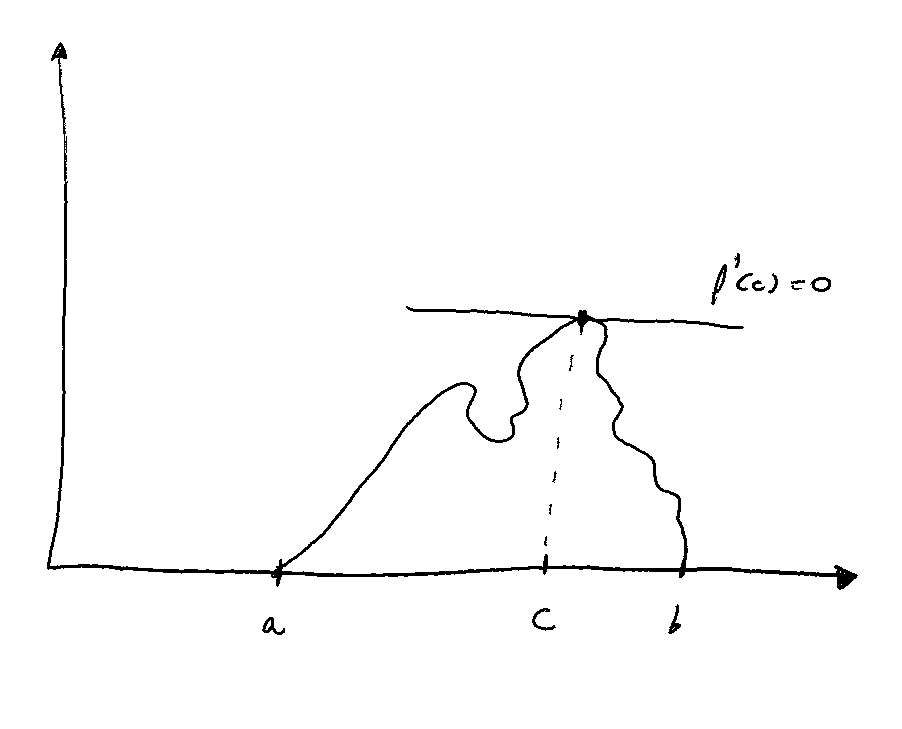
\includegraphics[scale=0.90]{Teorema de Rolle}
\end{center}
En caso contrario, $\exists x_0\in (a,b):f(x_0)\neq 0$. En primer lugar, supongamos que $f(x_0)>0\Rightarrow 0<f(x_0)\leq \max{f(x)}: x\in [a,b]$ y como $f$ es continua, entonces el máximo se alcanza por lo que $\exists c\in [a,b]: f(c)=\max{f(x)}>0\Rightarrow c\in (a,b): c\in \mathring{I}\Rightarrow f'(c) = 0$ por ser máximo relativo.

El caso menor es análogo.
\end{demo}

\begin{theo}[del valor medio]
Sea $f:[a,b]\rightarrow\mathbb R$ continua en $[a,b]$ y derivable en $(a,b)$, entonces:
$$\exists c \in (a,b): f'(c)=\frac{f(b)-f(a)}{b-a}$$
\end{theo}
\begin{demo}
Definimos la siguiente función $\psi(x)=\frac{f(b)-f(a)}{b-a}\cdot (x-a)-(f(x)-f(a))$. Vemos que reordenando las cosas tenemos:
$$\psi(x)=\underbrace{\frac{f(b)-f(a)}{b-a}\cdot (x-a)+f(a)}_{polinomio}-f(x)$$

Como $\psi$ es suma de funciones continuas y derivables, es continua y derivable. Además vemos que $\psi(a)=\frac{f(b)-f(a)}{b-a}\cdot (a-a)+f(a)-f(a)=0$ y que $\psi(b)=\frac{f(b)-f(a)}{b-a}\cdot (b-a)+f(a)-f(b)=0$ por lo que nos encontramos en las condiciones del teorema de Rolle, es decir:
$$\exists c\in (a,b): \psi'(c)=0\Rightarrow \frac{f(b)-f(a)}{b-a}-f'(c)=0\Rightarrow f'(c)=\frac{f(b)-f(a)}{b-a}$$
\end{demo}

\begin{obs}
Imponiendo las condiciones particulares del teorema de Rolle, este último engloba al anterior. A grandes rasgos viene a decir que existe un punto en el intervalo cuya recta tangente es precisamente una recta paralela a la que atraviesa $f(a)$ y $f(b)$.
\end{obs}

\begin{theo}
Sea $f:I\rightarrow\mathbb R$ una función continua y derivable en $\mathring{I}$, entonces:
\begin{enumerate}
\item $f$ es creciente si y sólo si $f'(x)\geq 0: \forall x\in \mathring{I}$
\item $f$ es decreciente si y sólo si $f'(x)\leq 0: \forall x\in \mathring{I}$
\end{enumerate}
\end{theo}
\begin{demo}
\begin{enumerate}
\item
	\begin{itemize}
	\item $\Rightarrow$
	
	Supongamos que $f$ es creciente. Sea $c\in \mathring{I}$, entonces $\exists \delta>0: (c-\delta, c+\delta)\subset I$. Podemos ver que $\frac{f(x)-f(c)}{x-c}\geq 0: \forall x\in I: x\neq c$ porque si es negativo denominador y numerador son negativos (en cuyo caso el cociente es positivo) y porque si son positivos ya ocurre trivialmente, así que ocurre que $f'(c)=\lim_{x\rightarrow c} \frac{f(x)-f(c)}{x-c} \geq 0$
	
	\item $\Leftarrow$
	
	Supongamos que $f'(x)\geq 0: \forall x \in \mathring{I}$. Sean $x_1<x_2: x_1,x_2\in I$. Sabemos que $f$ es continua en $I$ por lo que es continua en $[x_1,x_2])$ y además $f$ es derivable en $I$ por lo que es derivable en $(x_1,x_2)$. Por el teorema del valor medio se tiene que $\exists c\in (x_1,x_2): f'(c)=\frac{f(x_2)-f(x_1)}{x_2-x_1}$ y vemos que por hipótesis $f'(c)\geq 0$	
	\end{itemize}
	
\item Completamente análoga al punto 1.
\end{enumerate}
\end{demo}

\begin{coro}
Sea $f:I\rightarrow\mathbb R$ continua en $I$ y derivable en $\mathring{I}$, entonces:
\begin{itemize}
\item $\forall x\in \mathring{I}: f'(x)>0\Rightarrow f\mbox{ estrictamente creciente}$
\item $\forall x\in \mathring{I}: f'(x)<0\Rightarrow f\mbox{ estrictamente decreciente}$
\end{itemize}
Y el recíproco es falso, por ejemplo, $f(x)=x^3$
\end{coro}
\begin{demo}
Si $x_1<x_2$ como hemos hecho en la demostración del teorema anterior, aplicamos el teorema del valor medio a $f$ en $[x_1,x_2]$. Del mismo modo, el apartado 2 es totalmente análogo.
\end{demo}

\begin{obs}
Podríamos llegar a pensar que sea $f:I\rightarrow\mathbb R$ continua en $I$ y derivable en $\mathring{I}$ se tiene que si en un punto la derivada es estrictamente positiva implica que en los alrededores de ese punto la función es creciente, es decir:
$$f'(x_0)>0\Rightarrow \exists \delta>0: \forall x\in (x_0-\delta, x_0+\delta): f'(x)\geq 0$$
Lo que queremos decir es que si $x$ está muy cerca de $x_0$ entonces su derivada tiene que ser positiva, es decir:
$$0<f'(x)=\frac{f(x)-f(x_0)}{x-x_0}\Rightarrow\begin{cases}f(x)>f(x_0) & \mbox{ si }x>x_0\\ f(x)<f(x_0) & \mbox{ si }x<x_0)\end{cases}$$

Pero esto es completamente falso puesto que existen funciones que a pesar de ser derivables, continuas y en un punto crecientes, no se puede especificar ningún intervalo alrededor de ese punto que mantenga el crecimiento.
\end{obs}

\begin{ej}
Sea la función
$$f:\begin{cases}x+2x^2 \sen\left(\frac{1}{x}\right) & \mbox{ si }x\neq 0\\ 0 &\mbox{ si }x=0 \end{cases}$$
Vemos que es continua en $x\neq 0$ por composición de funciones continuas, pero ¿es continua en 0?:
$$\lim_{x\rightarrow 0} x+2x^2 \sen\left(\frac{1}{x}\right)$$
Vemos que
$$\left|x+2x^2 \sen\left(\frac{1}{x}\right)\right|\leq x+2x^2\xrightarrow{x\rightarrow 0} 0\Rightarrow x+2x^2 \sen\left(\frac{1}{x}\right)\xrightarrow{x\rightarrow 0}0$$ 

Ahora nos preguntamos ¿$f$ es derivable?, vemos fuera de $x=0$ como es composición de funciones derivables es derivable y concretamente es:
$$f'(x)=1+4x\sen\left(\frac{1}{x}\right)+2x^2\cos\left(\frac{1}{x}\right)\left(\frac{-1}{x^2}\right)=1+4x\sen\left(\frac{1}{x}\right)-2\cos\left(\frac{1}{x}\right)$$
Veamos ahora la derivada en 0:
$$f'(0)=\lim_{x\rightarrow 0}\frac{f(x)-f(0)}{x-0}=\lim_{x\rightarrow 0}\frac{x+2x^2\sen\left(\frac{1}{x}\right)}{x}=\lim_{x\rightarrow 0 }\left(1+2x\sen\left(\frac{1}{x}\right)\right)=1+0=1$$

Con lo cual, $f'(x)=\begin{cases}1+4x\sen\left(\frac{1}{x}\right)-2\cos\left(\frac{1}{x}\right) & x\neq 0\\ 1 & x=0\end{cases}$. Por lo tanto tenemos que a pesar de que la derivada en 0 es positiva, ocurre que para cualquier intervalo que escojamos alrededor de $0$ existen puntos donde la función crece y decrece, porque puedo escoger sucesiones que convergen a 0 pero cuya derivada es negativa y otras cuya derivada es positiva, por lo que no puedo afirmar nada sobre un intervalo alrededor de 0.
\end{ej}

\begin{prop}
Sea $f:I\rightarrow\mathbb R$ derivable en $x_0\in I$ tal que $f'(x_0)>0$, entonces:
$$\lim_{x\rightarrow x_0}\frac{f(x)-f(x_0)}{x-x_0}=f'(x_0)>0\Rightarrow \exists \delta>0, \ \forall x\in (x_0-\delta, x_0+\delta)\cap I\Rightarrow \frac{f(x)-f(x_0)}{x-x_0}>0$$
Por tanto, podemos deducir\footnote{Ocurre de modo análogo cuando $f'(x_0)<0$} que:
$$\begin{cases} x\in (x_0,x_0+\delta)\cap I &\Rightarrow f(x)>f(x_0)\\
x\in (x_0-\delta,x_0)\cap I & \Rightarrow f(x)<f(x_0)\end{cases}$$
\end{prop}
\begin{demo}
$$\lim_{x\rightarrow x_0}\frac{f(x)-f(x_0)}{x-x_0}=f'(x_0)>0\Rightarrow \varepsilon>0: \exists \delta>0 : 0<|x-x_0|<\delta\Rightarrow \left|\frac{f(x)-f(x_0)}{x-x_0} - f'(x_0)\right|<\varepsilon$$
Tomamos $\varepsilon = \frac{f'(x_0)}{2}>0$, luego:
$$\exists \delta>0 : 0<|x-x_0|<\delta\Rightarrow \left|\frac{f(x)-f(x_0)}{x-x_0} - f'(x_0)\right|<\frac{f'(x_0)}{2}\Rightarrow \frac{-f'(x_0)}{2}< \frac{f(x)-f(x_0)}{x-x_0} - f'(x_0)< \frac{f'(x_0)}{2}\Rightarrow $$
$$\Rightarrow 0< \frac{f'(x_0)}{2} <\frac{f(x)-f(x_0)}{x-x_0}<\frac{3}{2}f'(x_0)$$
\end{demo}

\begin{obs}
Lo que estamos diciendo es que si la derivada en un punto es positiva, entonces hay un entorno alrededor de dicho punto donde la función queda por debajo a la izquierda y queda por encima a su derecha del punto.

Esto no asegura que la derivada sea positiva, por lo tanto creciente, en un entorno alrededor del punto donde es positiva, sino más bien viene a afirmar que toda la parte derecha supera la imagen del punto y toda la izquierda no la supera.
\end{obs}

\begin{theo}
Sea $f:I\rightarrow \mathbb R$ una función continua\footnote{Cabe destacar que no se pide en ningún momento para aplicar este criterio que $c$ sea derivable.} en $c\in \mathring{I}$ y derivable en $(c-\delta,c+\delta)\setminus\{c\}$, entonces:
$$\forall x\in (c, c+\delta): f'(x)\geq 0 \mbox{ y } \forall x\in (c-\delta, c) : f'(x)\leq 0\Rightarrow c\mbox{ mínimo relativo}$$
$$\forall x\in (c, c+\delta) : f'(x)\leq 0 \mbox{ y } \forall x\in (c-\delta,c) : f'(x)\geq 0\Rightarrow c\mbox{ máximo relativo}$$
\end{theo}
\begin{demo}
Sea $x\in (c,c+\delta)$, por el teorema del valor medio tenemos que:
$$\frac{f(x)-f(c)}{x-c}=f'(z): z\in (c,x)\subset (c,c+\delta)\Rightarrow \frac{f(x)-f(c)}{x-c}\geq 0\Rightarrow f(x)\geq f(c)$$
De modo análogo, se tiene que sea $x\in (c-\delta,c)$, por el teorema del valor medio tenemos que:
$$\frac{f(x)-f(c)}{x-c}=f'(z): z\in (x,c)\subset (c-\delta,c)\Rightarrow \frac{f(x)-f(c)}{x-c}\leq 0\Rightarrow f(x)\geq f(c)$$
Lo que en conjunto implica que sea cual sea $x$ de ese intervalo, $f(x)\geq f(c)$, luego $c$ es un mínimo relativo.

La demostración del máximo es completamente análoga.
\end{demo}

\begin{theo}[de Darboux]
Sea $f:[a,b]\rightarrow \mathbb R$ derivable, la derivada toma todos los valores intermedios entre $f'(a)$ y $f'(b)$, es decir:
$$\forall k\in (f'(a), f'(b)) \mbox{ o } (f'(b), f'(a)): \exists c\in (a,b): f'(c)=k$$
\end{theo}

\begin{demo}
Supongamos $f'(a)<k<f'(b)$ y llamamos $g(x)=kx-f(x)$ y por ser diferencia de funciones continuas y derivables, entonces lo es en $[a,b]$. Entonces tenemos que $\exists c \in [a,b]: g(c)=\max{g(x)}: x\in [a,b]$ por el Teorema de Wiestrass. Veamos que:
$$g'(a)=k-f'(a)\stackrel{k>f'(a)}{\Rightarrow}g'(a)>0\Rightarrow \exists \delta>0: x\in (a, a+\delta)\Rightarrow g(x)>g(a)$$
Del mismo modo:
$$g'(b)=k-f'(b)<0\Rightarrow\exists \delta>0 : x\in (b-\delta, b)\Rightarrow g(x)>g(b)$$
Luego $c\neq a$ y $c\neq b$, por lo que $c\in (a,b)$ y $g'(c)=0\Rightarrow 0=g'(c)=k-f'(c)\Rightarrow f'(c)=k$

El otro caso es completamente análogo a lo anterior.
\end{demo}

\begin{obs}
Si $f'$ fuese continua, este teorema es trivial por el teorema del valor intermedio aplicado a $f'(x)$, pero el teorema no pide la condición de continuidad de la misma.
\end{obs}

\begin{obs}
Una consecuencia muy interesante de este teorema es que la función derivada puede no ser continua, pero en ningún caso puede tener saltos. Como concepto intuitivo, podemos decir que la discontinuidad posible que tienen es que oscile demasiado (como ocurre con $\sen\left(\frac{1}{x}\right)$).
$$DIBUJO$$
\end{obs}

\subsubsection{Aplicaciones del Teorema del valor Medio}
\underline{\textbf{Aproximaciones}}

Vamos a aproximar, por ejemplo, la raíz de 105. Sabemos que $\sqrt{100}=10$ y que $\sqrt{121}=11$ luego el número que buscamos debe estar entre 10 y 11. Entonces sea $f(x)=\sqrt{x}$ aplicamos el teorema del valor medio entre 100 y $105$:
$$\exists c\in (100, 105):f'(c)=\frac{f(105)-f(100)}{105-100}=\frac{\sqrt{105}-\sqrt{100}}{5}$$
Y también sabemos que $f'(c)=\frac{1}{2\sqrt{c}}$, luego se tiene que $\sqrt{105}=10+5f'(c)$. Si como hipótesis teníamos que $10<c<11$ es fácil llegar a que $\underbrace{10+\frac{5}{22}}_{\simeq 10,227}< \sqrt{105} < \underbrace{10+\frac{1}{4}}_{\simeq 10,25}$.

\underline{\textbf{Desigualdades}}

Vamos a probar que $\forall x \in \mathbb R: e^x \geq 1+x$. Es evidente que $1=e^0$ así que tomamos $f(x)=e^x$ luego por el teorema del valor medio se tiene que:
\begin{itemize}
\item $x>0$
$$\exists c\in (0,x): e^c=f'(c)=\frac{e^x-e^0}{x-0}\Rightarrow e^x-1=xe^c\stackrel{c>0}{\Rightarrow} e^x-1=xe^c>x\Rightarrow e^x>1+x$$

\item $x<0$
$$\exists c\in (x,0): e^c=f'(c)\frac{e^x-e^0}{x-0}\Rightarrow e^x-1=xe^c$$
Como $0<e^c<1$ y $x<0$, entonces $xe^x>x\Rightarrow e^x>1+x$

\item $x=0$
$$e^0=1+0$$
\end{itemize}

\subsection{Regla de L'Hopital}
Otro resultado notablemente importante es la regla de L'Hopital, pues simplificó el cálculo de límites bastante complejos a través de la derivación.

Para comprender la idea subyacente, supongamos $f,g: [a,b]\rightarrow \mathbb R$ de manera que $f(a)=0=g(a)$ y $g'(a)\neq 0$, entonces puedo transformar el límite del cociente como sigue:
$$\lim_{x\rightarrow a} \frac{f(x)}{g(x)}=\lim_{x\rightarrow a} \frac{f(x)-f(a)}{g(x)-g(a)}\Rightarrow \lim_{x\rightarrow a}\frac{\frac{f(x)-f(a)}{x-a}}{\frac{g(x)-g(a)}{x-a}}$$
Por tanto, si también pedimos que $f$ y $g$ sean derivables en $a$:
$$\lim_{x\rightarrow a} \frac{f(x)}{g(x)}=\frac{f'(a)}{g'(a)}$$

\subsubsection{L'Hôpital 1}
Sea $f,g: (a,b) \rightarrow \mathbb R$ donde $-\infty \leq a < b \leq \infty$, $f$ y $g$ derivables en $(a,b)$ con $g'(x)\neq 0: \forall x\in (a,b)$. Supongamos que $\lim_{x\rightarrow a^+} f(x)=\lim_{x\rightarrow a^+} g(x)=0$, si existe el $\lim_{x\rightarrow a^+} \frac{f'(x)}{g'(x)}=L\in \overline{\mathbb R}$ entonces $\lim_{x\rightarrow a^+}\frac{f'(x)}{g'(x)}=L$

\underline{Demostración}

Se basa en el siguiente resultado:

\underline{\textbf{Teorema del valor medio de Cauchy}}

Sean $f,g: [a,b]\rightarrow \mathbb R$ continuas en $[a,b]$ y derivables en $(a,b)$. Supongamos que $g'(x)\neq 0: \forall x\in (a,b)$, entonces $\exists c\in (a,b): \frac{f(b)-f(a)}{g(b)-g(a)}=\frac{f'(c)}{g'(c)}$.

Es fácil ver que si cogemos $g(x)=x$ recuperamos el enunciado que hemos visto del Teorema del valor Medio.

Demostración:

Sea $F:[a,b]\rightarrow\mathbb R$ definida como $F(x)=\frac{f(b)-f(a)}{g(b)-g(a)}\cdot (g(x)-g(a))\cdot (f(x)-f(a))$. De nuevo vemos que por ser suma de funciones continuas y derivables, F es continua en $[a,b]$ y derivable en $(a,b)$ y además $(g(x)-g(a))\neq 0$ porque por el teorema de valor medio ocurriría que $g(b)=g(a)\Rightarrow \exists c\in  (a,b): g'(c)=0\Rightarrow \#$ porque hemos dicho que $g'(x)\neq 0$.

Además ahora tenemos que $F(b)=F(a)=0$, por lo que por el Teorema de Rolle tenemos que $\exists c \in (a,b): F'(c)=0\Rightarrow \frac{f(b)-f(a)}{g(b)-g(a)}=\frac{f'(c)}{g'(c)}$.

Volviendo a la demostración inicial, vamos a ver el caso en que $L\in \mathbb R$. Por la definición de límite tenemos que:
$$\forall \varepsilon>0: \exists c\in (a,b): x\in (a,c)\Rightarrow \left|\frac{f'(x)}{g'(x)}-L\right|\Leftrightarrow L-\varepsilon< \frac{f'(x)}{g'(x)}< L+\varepsilon$$
Vamos a escoger $a<\alpha<\beta < c$, entonces vemos que $f,g: [\alpha,\beta]\rightarrow \mathbb R$ y cumplen las hipótesis del Teorema visto antes, así que:
$$\frac{f(\beta)-f(\alpha)}{g(\beta)-g(\alpha)}=\frac{f'(u)}{g'(u)}: u\in (\alpha, \beta)$$
FALTA ALGUNA COSILLA DE EXPLICACIÓN

Entonces si $a<\alpha < \beta < c$, se tiene que:
$$L-\varepsilon< \frac{f(\beta)- f(\alpha)}{g(\beta)-g(\alpha)}<L+\varepsilon$$

Vamos a fijar $\beta$ y vamos a acercar $\alpha $ cada vez más a $a$, por lo tanto podemos pasar al límite cuando $\alpha \rightarrow a$:
$$\frac{f(\beta)-f(\alpha)}{g(\beta)-g(\alpha)}\xrightarrow{\alpha\rightarrow a^+} \frac{f(\beta)}{g(\beta)}$$
FALTA EXPLICACIONES IMPORTANTES DE MOVER PARÁMETROS

Como $L-\varepsilon < \frac{f(\beta)- f(\alpha)}{g(\beta)-g(\alpha)}<L+\varepsilon$ cuando $\alpha \rightarrow a^+$ tenemos que:
$$L-\varepsilon \leq \frac{ f(\beta)}{g(\beta)}\leq L+\varepsilon\Rightarrow \left|\frac{f(\beta)}{g(\beta)}-L\right|<\varepsilon: \forall a<\beta, c$$
Luego precisamente esto es la definición de límite:
$$\lim_{\beta\rightarrow a^+}\frac{f(\beta)}{g(\beta)}$$

Para cambiar la demostración para que sea $L\in \overline{\mathbb R}$ entonces:

CAMBIA COSAS QUE NO HE VISTO.

\subsubsection{L'Hôpital 2}
Sea $-\infty\leq a < b \leq \infty$, $f,g: [a,b]\rightarrow \mathbb R$ derivables en $(a,b)$, supongamos que $g'(x)\neq 0: \forall x\in (a,b)$ y $\lim_{x\rightarrow a^+}g(x)=\pm\infty$, entonces:
$$\lim_{x\rightarrow a^+}\frac{f(x)}{g(x)}=\lim_{x\rightarrow a^+}\frac{f'(x)}{g'(x)}=L\in \overline{\mathbb R}$$

\underline{Demostración}:

La demostración es muy parecido a lo anterior y se deja para mirar en los libros en caso de no saber hacerla.

\subsubsection{Ejemplos de aplicación del Teorema de L'Hôpital}
Supongamos que $\lim_{x\rightarrow \infty} e^{-x} \cdot x^2$, es fácil ver que nos queda una indeterminación de tipo $\frac{\infty}{\infty}$ porque se puede reescribir $\lim_{x\rightarrow \infty}\frac{x^2}{e^x}$. Como se cumplen las hipótesis de L'Hopital podemos hacer:
$$\lim_{x\rightarrow \infty} e^{-x} \cdot x^2=\lim_{x\rightarrow \infty}\frac{x^2}{e^x}\stackrel{\mbox{L'Hôpital}}{=}\lim_{x\rightarrow \infty}\frac{2x}{e^x}\stackrel{\mbox{L'Hôpital}}{=}\lim_{x\rightarrow \infty}\frac{2}{e^x}=0$$

Supongamos que $\lim_{x\rightarrow \infty}\frac{ln(x)}{x}$ que de nuevo nos queda la indeterminación de $\frac{\infty}{\infty}$, como se cumplen las hipótesis digo:
$$\lim_{x\rightarrow \infty} \frac{ln(x)}{x}=\lim_{x\rightarrow \infty}\frac{\frac{1}{x}}{1}=\lim_{x\rightarrow \infty}\frac{1}{x}=0$$

Veamos el caso $\lim_{x\rightarrow \infty} e^{-\alpha \cdot x}\cdot x^n$, la pregunta es saber si habrá valores de $\alpha$ o de $n$ para los que pasen cosas distintas (¿quién gana?):
$$\lim_{x\rightarrow \infty} e^{-\alpha x}x^n=\lim_{x\rightarrow \infty}\frac{x^n}{e^{\alpha x}}=\lim_{x\rightarrow \infty} \frac{n\cdot x^n}{\alpha e^{\alpha x}}=\cdots =\lim_{x\rightarrow \infty} \frac{n!}{\alpha^n e^{\alpha x}}=0$$

\section{Otros Resultados}
Por último, vamos a mencionar un par enunciados muy importantes, consecuencia de la teoría desarrollada a lo largo de todo el capítulo. Es muy destacable sobre todo el \textit{Teorema de Taylor} por su repercusión en la sección \nameref{Series de Funciones} y por la cantidad de aplicaciones que tiene en general. 

\subsection{Teorema de Taylor}
Supongamos que tenemos una función $f:\mathbb R\rightarrow \mathbb R$, un hecho difícil de adivinar, pero sencillo de entender es que la recta tangente es la que mejor aproxima a la función en un punto:
\begin{center}
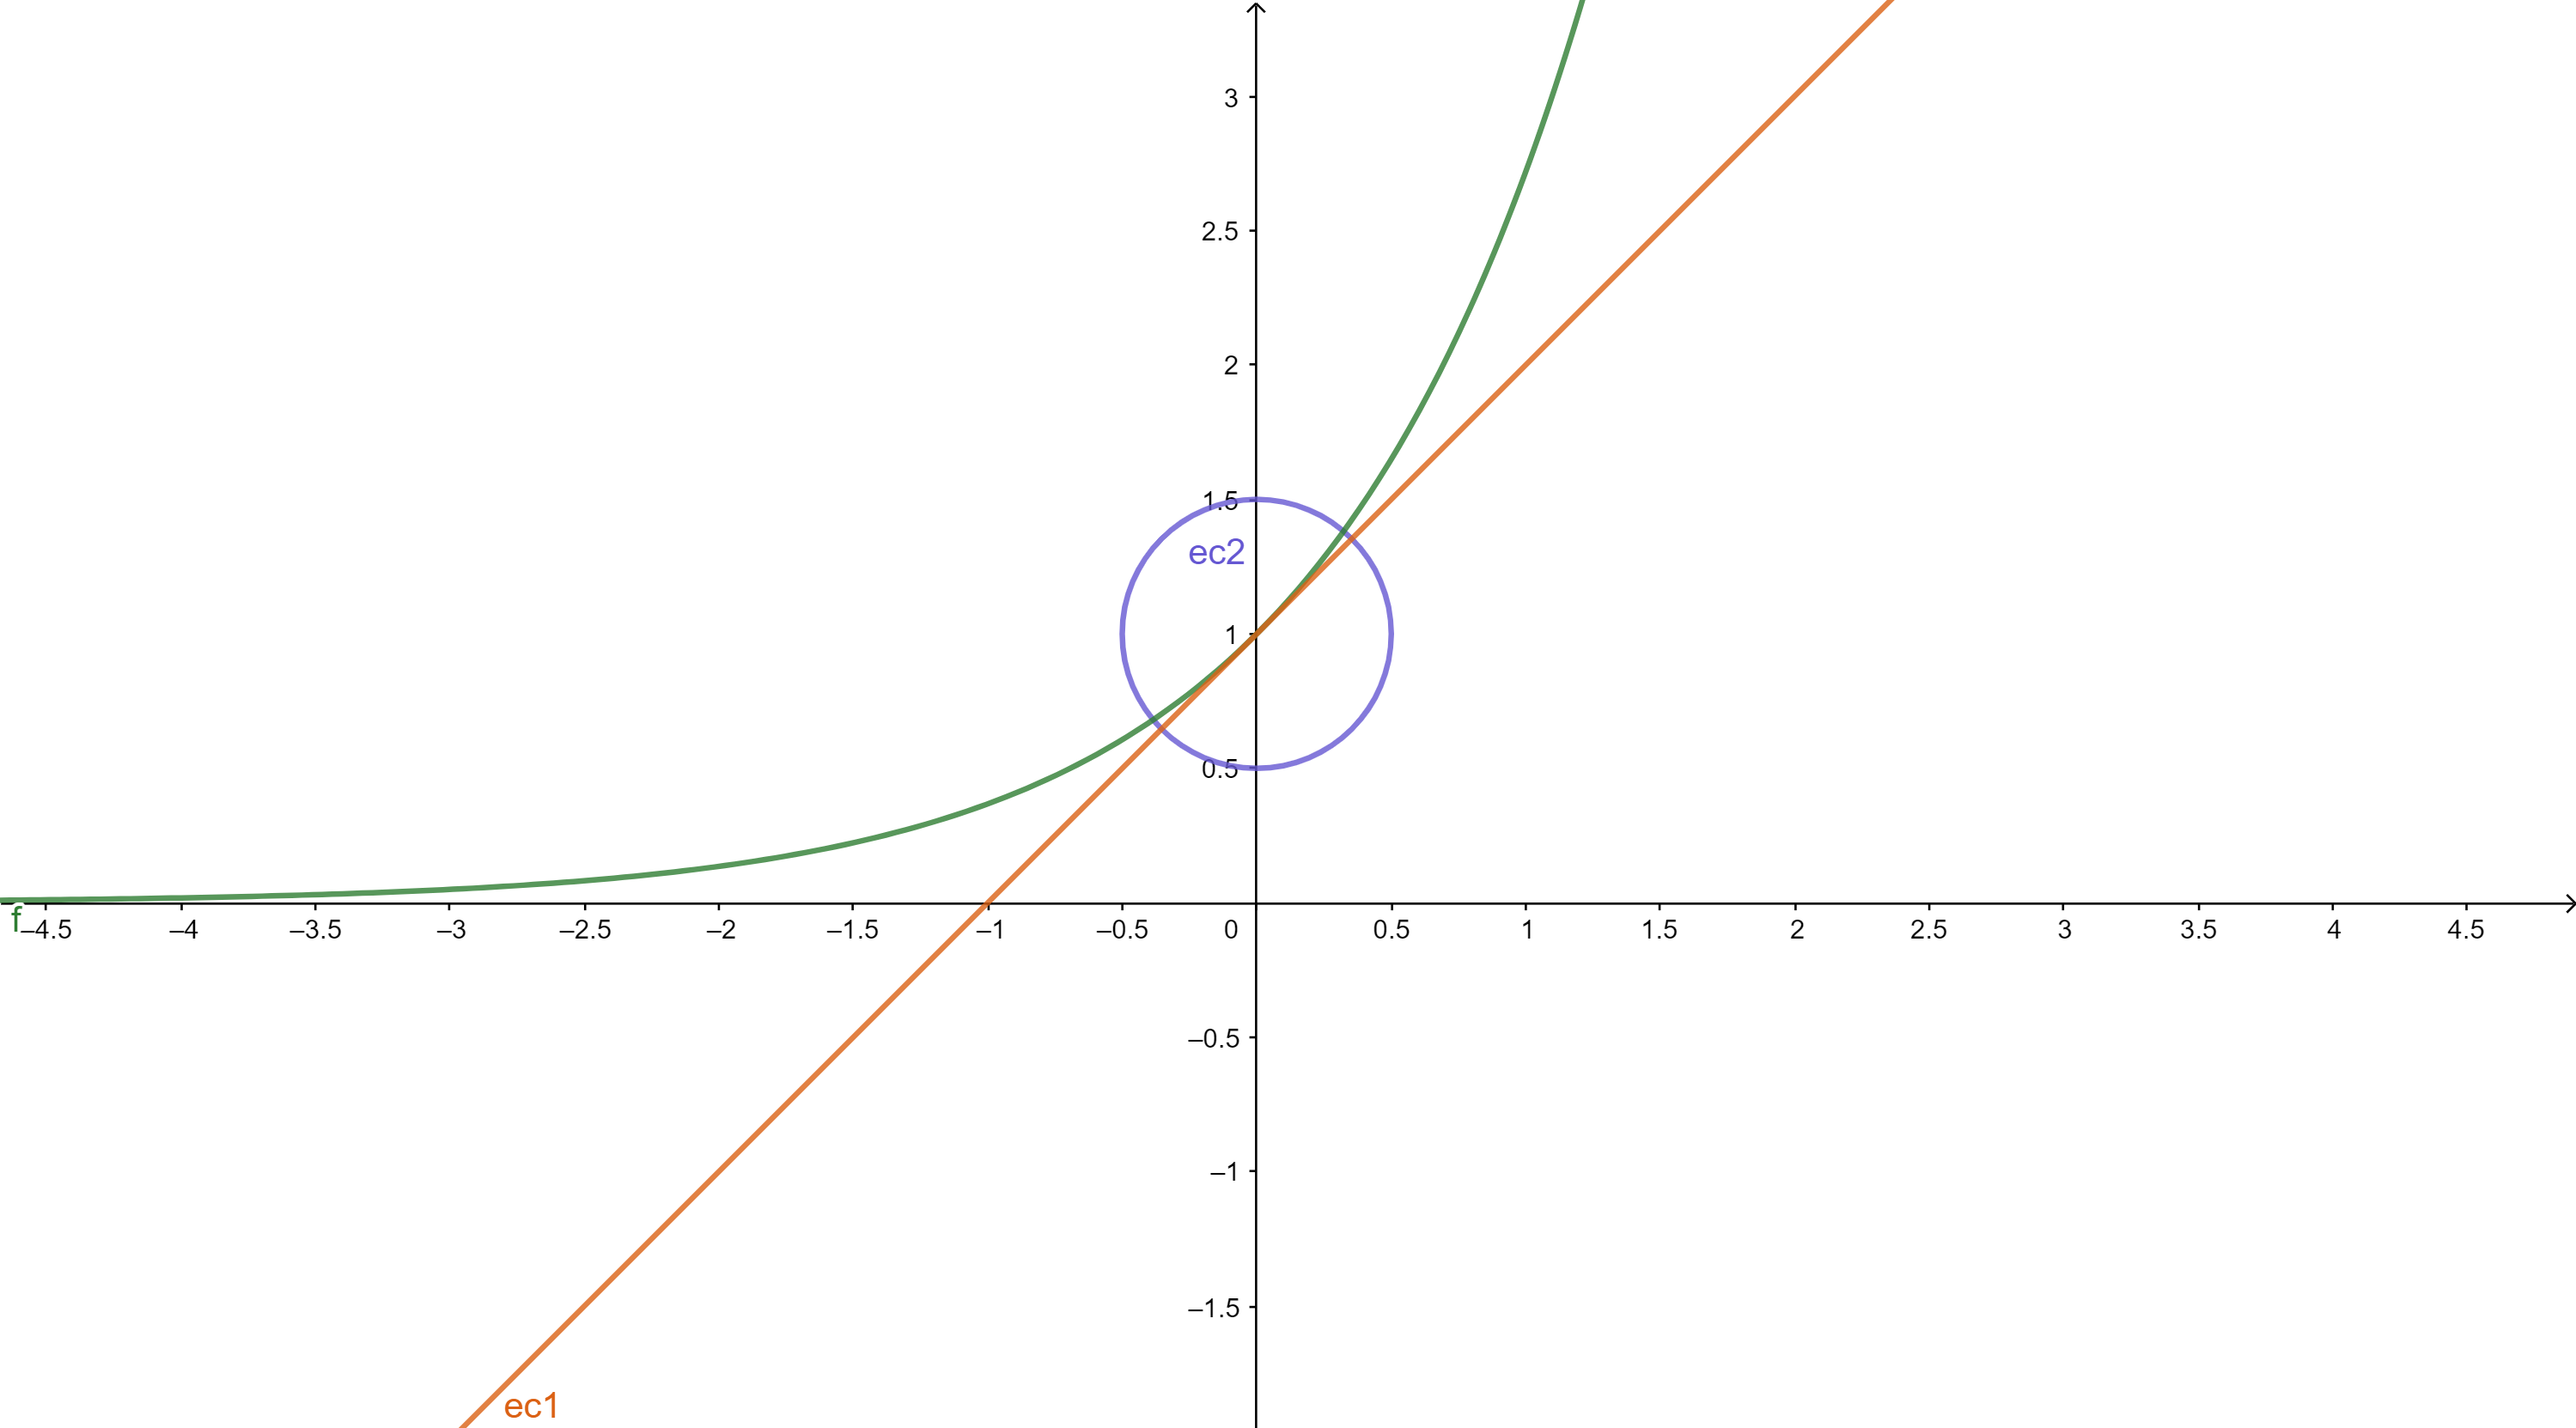
\includegraphics[scale=0.9]{polinomio de taylor 1}
\end{center}
Incluso ampliando, vemos que de todas las rectas posibles que atraviesan ese punto, la tangente es la que más ``se parece'' a la función que tenemos:
\begin{center}
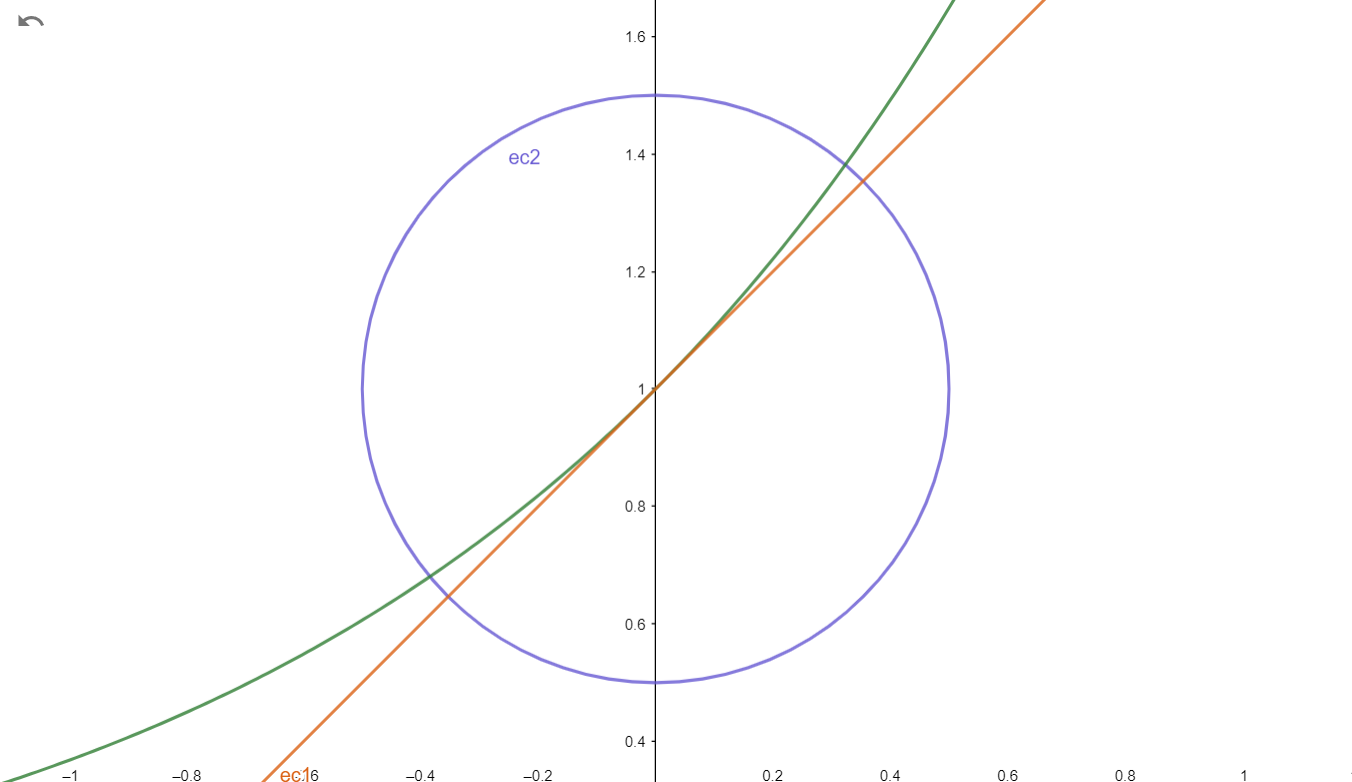
\includegraphics[scale=0.25]{de taylor 2}
\end{center}
Y, en consecuencia, surge la siguiente pregunta ¿cuál será el polinomio de grado 2 que mejor aproxime a $f$?, y todavía más en general, ¿cuál será el polinomio de grado $n$ que mejor aproxima a la función $f$?.

Una de las ideas más razonable desde un principio es pensar en el polinomio de grado 2 que verifique:
\begin{align*}
p(x_0)=f(x_0)  & &
p'(x_0)=f'(x_0) & &
p''(x_0)=f''(x_0)
\end{align*}
Y viendo las condiciones que imponemos, también es razonable querer escribir el polinomio en cuestión $p(x)=a_0+a_1x+a_2x^2$ en términos de $x_0$ o, mejor dicho, centrado en $x_0$, es decir:
$$p(x; x_0)=b_0+b_1(x-x_0)+b_2(x-x_0)^2$$
Ahora basta con determinar los coeficientes $b_i$ imponiendo las condiciones iniciales sobre dicho polinomio:
$$\begin{cases} p(x_0)=b_0+0+0=b_0=f(x_0)&\Rightarrow b_0=f(x_0)\\
p'(x_0)=b_1+2b_2(x_0-x_0)=b_1=f'(x_0)&\Rightarrow b_1=f'(x_0)\\
p''(x_0)=2b_2=f''(x_0)&\Rightarrow b_2= \frac{f''(x_0)}{2}\end{cases}$$
Luego el polinomio queda como
$$p(x)=f(x_0)+f'(x_0)(x-x_0)+\frac{f''(x_0)}{2}(x-x_0)^2$$

Por tanto, es razonable pensar que, en el caso general, concluimos que el único polinomio de grado $n$ tal que $p_n(x_0)=f(x_0)$, $p_n'(x_0)=f'(x_0)$, ..., $p_n^{(n)}(x_0)=f^{(n)}(x_0)$ es precisamente el polinomio de Taylor que vamos a definir.

\begin{defi}[Polinomio de Taylor]
Sea $f: I\rightarrow \mathbb{R}$ una función cuyas derivadas $f'(x), f''(x), \cdots, f^{(n)}(x)$ existen y son continuas en $I$, definimos su \textbf{polinomio de Taylor de grado $n$} como:
$$p_n(x; x_0)=f(x_0)+f'(x_0)(x-x_0)+\frac{f''(x_0)}{2}(x-x_0)^2+\frac{f'''(x_0)}{3!}(x-x_0)^3+ \cdots +\frac{f^{(n)}(x_0)}{n!}(x-x_0)^n$$
\end{defi}

\begin{obs}
Habría que comprobar que la definición que se ha dado cumple que $p_n(x_0)=f(x_0)$, $p_n'(x_0)=f'(x_0)$, ..., $p_n^{(n)}(x_0)=f^{(n)}(x_0)$.
\end{obs}

\begin{theo}[de Taylor]
Sea $I=[a,b]$ un intervalo, $f:I\rightarrow \mathbb R$ una función cuyas $f,f',f'', ..., f^{(n)}$ existen y son continuas en $I$ y $f^{(n+1)}$ existe en $\mathring{I}$, entonces\footnote{El resto de Lagrange el error que existe entre la aproximación del polinomio de Taylor y la función requerida} $\forall x_0 \in [a,b]$:
$$\forall x\in I: f(x)=p_n(x; x_0)+\underbrace{\frac{f^{(n+1)}(c)}{(n+1)!}\cdot (x-x_0)^{n+1}}_{\text{Resto de Lagrange ($R_n$)}}$$
Donde $c\in (x,x_0)\cup (x_0, x)$ y, por tanto, depende de $x_0, x, n, f$.
\end{theo}
\begin{demo}
Definimos la función $F(t)$ con $t\in I$ de la siguiente forma:
$$F(t)=f(x)-\left[f(t)+f'(t)(x-t)+\frac{f''(t)}{2}(x-t)^2+\cdots + \frac{f^{(n)}(t)}{n!}(x-x_0)^n\right]=f(x)-p_n(x;t)$$
Vemos entonces que ocurre que $F(x)=f(x)-f(x)=0$, que $F(x_0)=f(x_0)-p_n(x;x_0)$ y que además es continua y derivable. Veamos su derivada:
$$F'(t)=-\left[\cancel{f'(t)}+\cancel{f''(t)(x-t)}\cancel{-f'(t)}+\cancel{\frac{f'''(t)}{2!}(x-t)^2}+\cancel{\frac{f''(t)}{2!}2(x-t)(-1)}+\cancel{\cdots} +  \frac{f^{(n-1)}(t)}{n!}(x-t)^n\right] $$
$$= -\frac{f^{(n-1)}(t)}{n!}(x-t)^n$$
Se va todo con todo porque es como una suma telescópica, cada término se anula con el siguiente al siguiente menos el último que se queda sin pareja para irse.

Ahora vamos a definir otra función que llamaremos $G(t)=(x-t)^{n+1}$ y ahora vamos a aplicar el Teorema del valor medio de Cauchy porque $G$ es derivable y su derivada es distinta de 0 en cualquier valor de $t$:
$$\exists c \in (x_0,x)\vee (x,x_0): \frac{F(x)-F(x_0)}{G(x)-G(x_0)}=\frac{F'(c)}{G'(c)}\Rightarrow \frac{F(x_0)}{G(x_0)}=\frac{F'(c)}{G'(c)}\Rightarrow F(x_0)=G(x_0)\frac{F'(c)}{G'(c)}=$$
$$=(x-x_0)^{n+1}\cdot \frac{-f^{(n+1)}(c)(x-c)^n}{-1\cdot n!(n+1)(x-c)^n}\Rightarrow f(x)-p_n(x;x_0)=R_n$$
\end{demo}

\begin{obs}
Como observación, si escogemos $n=0$ entonces quedaría como $f(x)=p_n+R_n=f(x_0)+f'(c)(x-x_0)\Rightarrow \frac{f(x)-f(x_0)}{x-x_0}=f'(c)$ que es justamente el Teorema del Valor Medio, así que podemos considerar que este teorema es como una generalización del teorema del Valor Medio.
\end{obs}


\subsubsection{Aplicaciones del Teorema de Taylor}
Veamos el caso de $f(x)=e^x$, ocurre que $f'(x)=e^x$ y en particular $\forall n\in \mathbb N : f^{(n)}(x)=e^x$ , si tomamos $x_0=0$, entonces $f(0)=1=f'(0)=f''(0)=\cdots = f^{(n)}(0)$ y el polinomio de taylor queda como:
$$e^x=\underbrace{1+x+\frac{1}{2}x^2+\frac{1}{3!}x^3+\cdots + \frac{1}{n!}x^n}_{p_n(x;0)}+\underbrace{\frac{e^c}{(n+1)!}x^{n+1}}_{R_n(x;0)}$$
¿Pero para qué sirve esto? Pues vamos a aproximar el número $e$:
$$x=1\Rightarrow e=1+\frac{1}{2}+\frac{1}{3!}+\cdots + \frac{1}{n!}+\frac{e^c}{(n+1)!}$$
Ahora como $c$ depende de $n$ dando valores vamos a obtener sucesivas aproximaciones cada vez más refinadas:
$$0< e-(1+\frac{1}{2}+\frac{1}{3!}+\cdots + \frac{1}{n!})=\frac{e^c}{(n+1)!}\leq \frac{e}{(n+1)!}\leq \frac{3}{(n+1)!}$$
Con lo cual despejando $e$ y ya que lo tenemos acotado, podemos dar valores de $n$ cada vez más grandes para que quede más acotado.

\begin{ej}
¿Qué valor tiene que tomar $n$ para aproximar $e$ con un error menor que $10^5$?
$$\frac{3}{(n+1)!}<10^5\Rightarrow n>8$$
\end{ej}

\begin{prop}
Sea $I$ un intervalo, $x_0\in \mathring{I}$ y $f:I\rightarrow \mathbb R$ tal que $\exists f, f', f'', ..., f^{(n)}$ son continuas en un entorno de $x_0$. Si $f'(x_0)=f''(x_0)=\cdots = f^{(n-1)}(x_0)=0$ y $f^{(n)}(x_0)\neq 0$, entonces:
\begin{itemize}
\item $n$ es par y $f^{(n)}(x_0)>0\Rightarrow x_0$ es mínimo relativo estricto
\item $n$ es par y $f^{(n)}(x_0)<0 \Rightarrow x_0$ es máximo relativo estricto

\item $n$ es impar, entonces el punto no es ni máximo ni mínimo
\end{itemize}
\end{prop}
\begin{demo}
Por el Teorema de Taylor:
$$f(x)=p_{n-1}(x;x_0)+R_{n-1}(x;x_0)=f(x_0)+f'(x_0)(x-x_0)+\cdots + \frac{f^{(n-1)}(x_0)}{(n-1)!}(x-x_0)^{n-1}+\frac{f^{(n)}(c)}{n!}(x-x_0)^n$$
Por las hipótesis de que todas las derivadas menos la enésima son nulas tenemos que:
$$\forall x\in (x_0-\delta, x_0+\delta): f(x)=f(x_0)+\frac{f^{(n)}}{n!}(x-x_0)^n$$
Lo importante es pensar ahora que ocurre realmente cuando la $x$ se asemeja mucho a la $x_0$. Como $f^{(n)}(x_0)\neq 0$, entonces si $f^{(n)}(x_0)>0$ como $f^{(n)}$ es continua en $(x_0-\delta, x_0+\delta)$, entonces $\exists \delta' < \delta: \forall x\in (x_0-\delta', x_0+\delta'): f^{(n)}(x)>0$.

Entonces para $0<|x-x_0|<\delta'$, entonces puedo escoger el $c\in (x_0-\delta', x_0+\delta')\Rightarrow f^{(n)}(c)>0$, de forma similar ocurre que $f^{(n)}(x_0)<0\Rightarrow f^{(n)}(c)<0$ así que volviendo a $f(x)$:
\begin{itemize}
\item $n$ par y $f^{(n)}(x_0)>0$ para $x\in (x_0-\delta', x_0+\delta')$.
$$f(x)=f(x_0)+\underbrace{\frac{f^{(n)}}{n!}(x-x_0)^n}_{>0}\Rightarrow f(x)>f(x_0)\Rightarrow x_0\mbox{ mínimo}$$

\item $n$ par y $f^{(n)}(x_0)<0$ para $x\in (x_0-\delta', x_0+\delta')$
$$f(x)=f(x_0)+\underbrace{\frac{f^{(n)}}{n!}(x-x_0)^n}_{<0}\Rightarrow f(x)<f(x_0)\Rightarrow x_0\mbox{ máximo}$$

\item $n$ impar
$$f(x)=f(x_0)+\underbrace{\frac{f^{(n)}}{n!}(x-x_0)^n}_{???}$$
Como ahora $f^{(n)}(c)$ es fijo el término que no podemos determinar el signo que toma lo demás y en consecuencia no puede ser máximo ni mínimo. 
\end{itemize}
\end{demo}

\begin{prop}
El polinomio de Taylor aproxima a la función mejor que cualquier otro polinomio, es decir, sea $f: I\rightarrow\mathbb R$ tal que $f, f'', ..., f^{(n)}, f^{(n+1)}$ son continuas y $x_0\in \mathring{I}$. Si llamamos $Q_n(x)$ a cualquier otro polinomio de grado $\leq n$, entonces:
$$\lim_{x\rightarrow x_0}\frac{|f(x)-p_n(x;x_0)|}{|f(x)-Q_n(x)|}=0$$\end{prop}
\begin{demo}
$$f(x)-p_n(x;x_0)=\frac{f^{(n+1)}(c)}{(n+1)!}(x-x_0)^{n+1}$$
Como en particular es continua en un entorno de $x_0$, lo anterior va a estar acotado. Fijamos un $\delta_0>0 : [x_0-\delta_0, x_0+\delta_0]\in I$ y si $M_{n+1}=\max |f^{(n+1)}(x)|$ donde $|x-x_0|<\delta$. Es decir, que llamo $M_{n+1}$ a la máxima derivada del orden $n+1$ de las $x$ en ese entorno alrededor de $x_0$. 

Por tanto:
$$x\in [x_0-\delta_0, x_0+\delta_0]\Rightarrow c\in [x_0-\delta_0, x_0+\delta_0] \Rightarrow |f^{(n+1)}(c)|\leq M_{n+1}$$
Y en consecuencia:
$$x\in [x_0-\delta_0, x_0+\delta_0]\Rightarrow |f(x)-p_n(x;x_0)|\leq \underbrace{\frac{M_{n+1}}{(n+1)!}}_{cte}|x-x_0|^{n+1}$$
Por otro lado, si $p_n(x;x_0)=p_0+p_1(x-x_0)+\cdots +p_n(x-x_0)^n$ y $Q_n(x)=q_0+q_1(x-x_0)+\cdots +q_n(x-x_0)^n$ como deben ser distintos:
$$Q_n\neq p_n\Rightarrow \exists i_0\in \{0, ..., n\}: p_{i_0}\neq q_{i_0}\wedge p_i=q_i:\forall i < i_0$$
Por tanto:
$$p_n(x;x_0)-Q_n(x)=(p_{i_0}-q_{i_0})(x-x_0)^{i_0}+(p_{i_0+1}-q_{i_0+1})(x-x_0)^{i_0+1}+\cdots + (p_n-q_n)(x-x_0)^{n}\Rightarrow $$
$$\Rightarrow p_n(x;x_0)-Q_n(x)=(p_{i_0}-q_{i_0})(x-x_0)^{i_0}\left( 1+ \frac{p_{i_0+1}-q_{i_0+1}}{p_{i_0}-q_{i_0}}(x-x_0)+\cdots + \frac{p_n-q_n}{p_{i_0}-q_{i_0}}(x-x_0)^{n-i_0}\right)$$
Como todos los términos de dentro del paréntesis excepto el uno van a 0, entonces podemos escoger un delta de manera que sean más pequeños que $\frac{1}{2}$:
$$\delta_1< \delta_0: |x-x_0|<\delta_1\Rightarrow \left| \frac{p_{i_0+1}-q_{i_0+1}}{p_{i_0}-q_{i_0}}(x-x_0)+\cdots + \frac{p_n-q_n}{p_{i_0}-q_{i_0}}(x-x_0)^{n-i_0}\right|\leq \frac{1}{2}$$
Entonces para tratar de acotarlo:
$$|x-x_0|<\delta_1\<\Rightarrow|p_n(x;x_0)-Q_n(x)|=|p_{i_0}-q_{i_0}||x-x_0|^{i_0}\underbrace{\left| 1 + \cdots \right|}_{\geq \frac{1}{2}}\geq \frac{|p_{i_0}-q_{i_0}|}{2}|x-x_0|^{i_0}$$

Entonces para los $|x-x_0|<\delta_1$ tenemos dos estimaciones, queremos ver esto:
$$|x-x_0|<\delta_1\Rightarrow\frac{|f(x)-p_n(x;x_0)|}{|f(x)-Q_n(x)|}$$
Por un lado:
$$|f(x)-Q_n(x)|=|f(x)-Q_n(x)+p_n(x;x_0)-p_n(x;x_0)|\geq |p_n(x;x_0)-Q_n(x)|-|f(x)-p_n(x;x_0)|\geq $$
$$\geq \frac{|p_{i_0}-q_{i_0}|}{2}|x-x_0|^{i_0} - \frac{M_{n+1}}{(n+1)!}|x-x_0|^{n+1}$$
Y esto último es siempre positivo porque cuando $x\rightarrow x_0$ el término $n+1$ se hace pequeño mucho más rápido que el término $i_0$ (la demostración es sacar factor común). Pues con numerador y denominador acotado puedo escribir que:
$$=\frac{|f(x)-p_n(x;x_0)|}{|f(x)-Q_n(x)|}\leq \frac{\frac{M_{n+1}}{(n+1)!}|x-x_0|^{n+1}}{|x-x_0|^{i_0}\left( \frac{|p_{i_0}-q_{i_0}|}{2} - \frac{M_{n+1}}{(n+1)!}|x-x_0|^{n-i_0+1} \right)} = \frac{\frac{M_{n+1}}{(n+1)!}|x-x_0|^{n-i_0+1}}{\frac{|p_{i_0}-q_{i_0}|}{2} - \frac{M_{n+1}}{(n+1)!}|x-x_0|^{n-i_0+1}}$$
Y es trivial ver que cuando $x\rightarrow x_0$ el denominador tiende a una constante y el numerador tiende a 0, luego el resultado de pasar al límite es 0 por la regla del sandwich (porque ese cociente es positivo).
\end{demo}

\subsection{Convexidad y Concavidad}
De forma intuitiva, decimos que una función es convexa cuando tiene la forma de ``una sonrisa'' y ocurre siempre que los dos puntos de la función en un intervalo $I$ la gráfica de la función quedan por arriba o por debajo de la recta.

\begin{center}
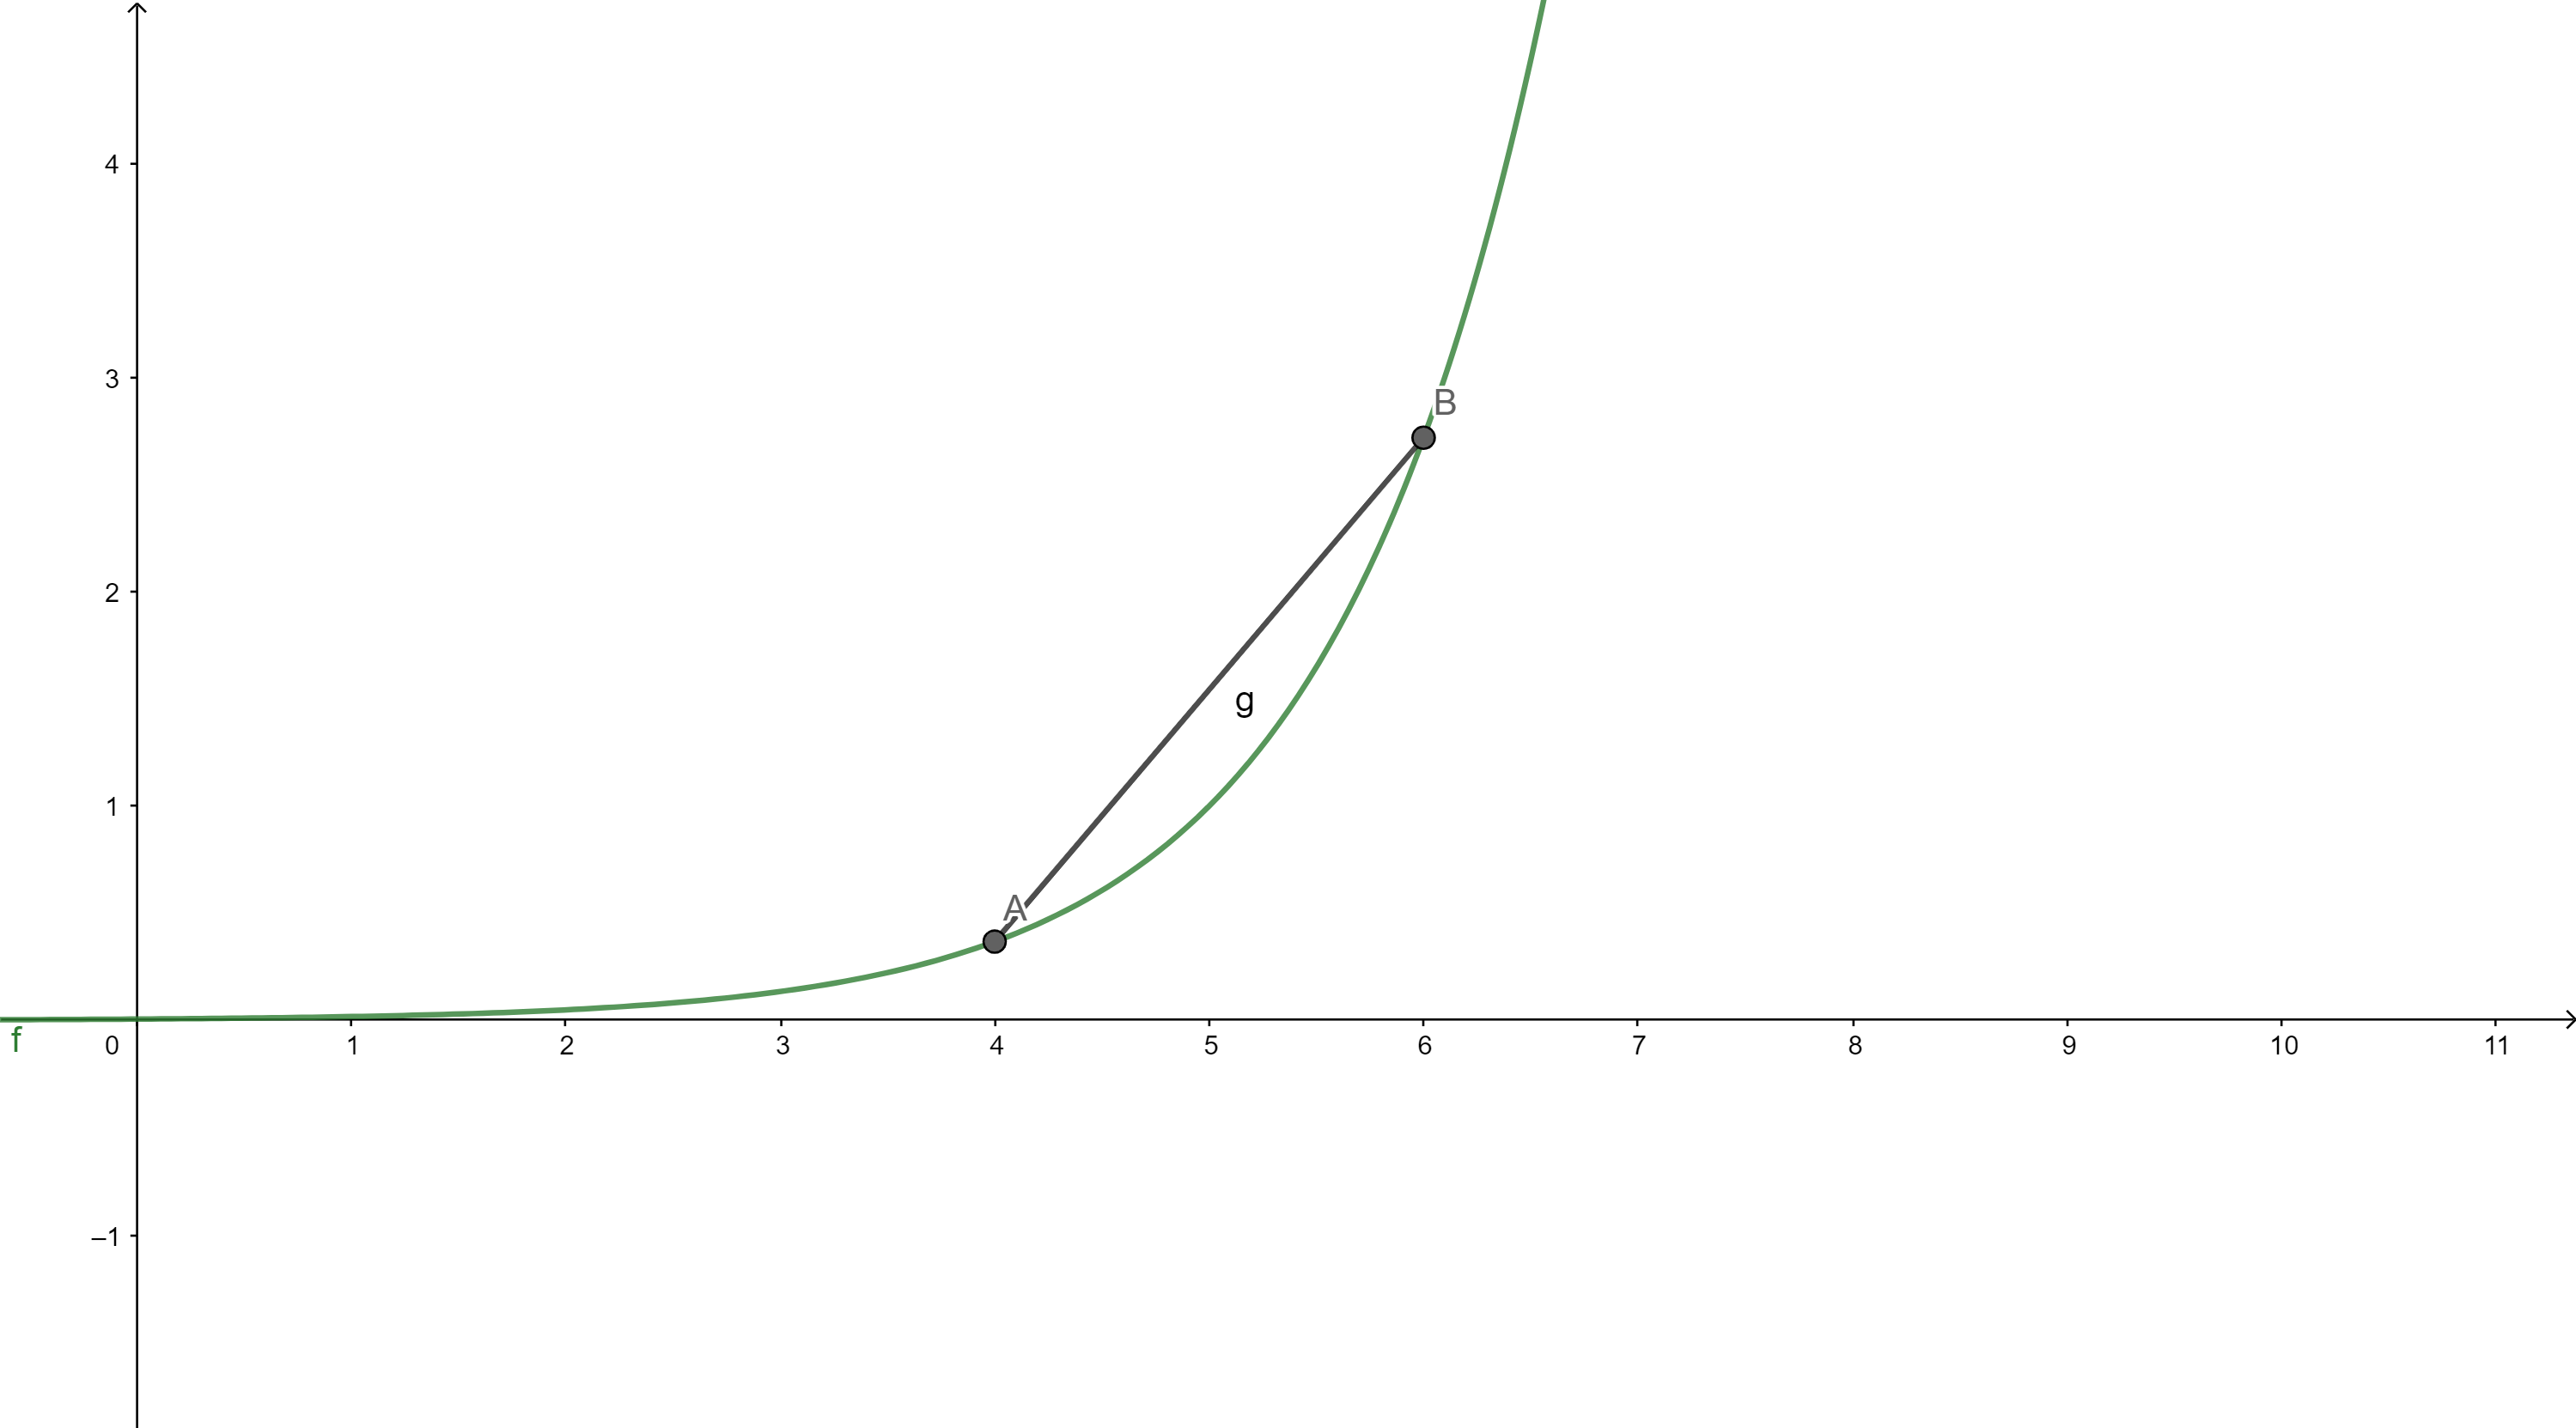
\includegraphics[scale=0.70]{convexidad}
\end{center}

\begin{defi}[Convexidad]
Sea $f:I\rightarrow\mathbb R$, decimos que es \textbf{convexa} si\footnote{Para los valores de $t=0$ y $t=1$ la desigualdad es trivial} y sólo si:
$$\forall x_0,x_1 \in I: \forall t\in (0,1): f(tx_0+(1-t)x_1)\leq f(x_0)+(1-t)f(x_1)$$
\end{defi}

Para ver la interpretación que le podemos dar a dicha definición, supongamos que tenemos $x_0, x_1\in I$ tal que $x_0<x_1$, sin pérdida de generalidad, y $t\in (0,1)$. Veamos que siempre $tx_0+(1-t)x_1\in (x_0, x_1)$:
$$tx_0+(1-t)x_1=x_0-x_0+tx_0+(1-t)x_1= x_0 +\underbrace{(1-t)(x_1-x_0)}_{>0}\Rightarrow x_0\leq tx_0+(1-t)x_1\leq \underbrace{x_0+(x_1-x_0)}_{=x_1}$$
Además cabe destacar que cualquier punto entre ambos puntos se puede escribir de esta forma tomando un cierto valor de $t$:
$$z\in (x_0,x_1)\Rightarrow z= x_0+\frac{z-x_0}{x_1-x_0}(x_1-x_0)= x_0+\frac{z-x_1+x_1-x_0}{x_1-x_0}(x_1-x_0)=$$
$$=x_0+(1-\underbrace{\frac{x_1-z}{x_1-x_0}}_{=t})(x_1-x_0)= x_0+(1-t)(x_1-x_0)$$

\textbf{A la expresión} $tx_0+(1-t)x_1: t\in (0,1)$ \textbf{se le denomina combinación lineal convexa de} $x_1$ \textbf{y} $x_2$.

\begin{center}
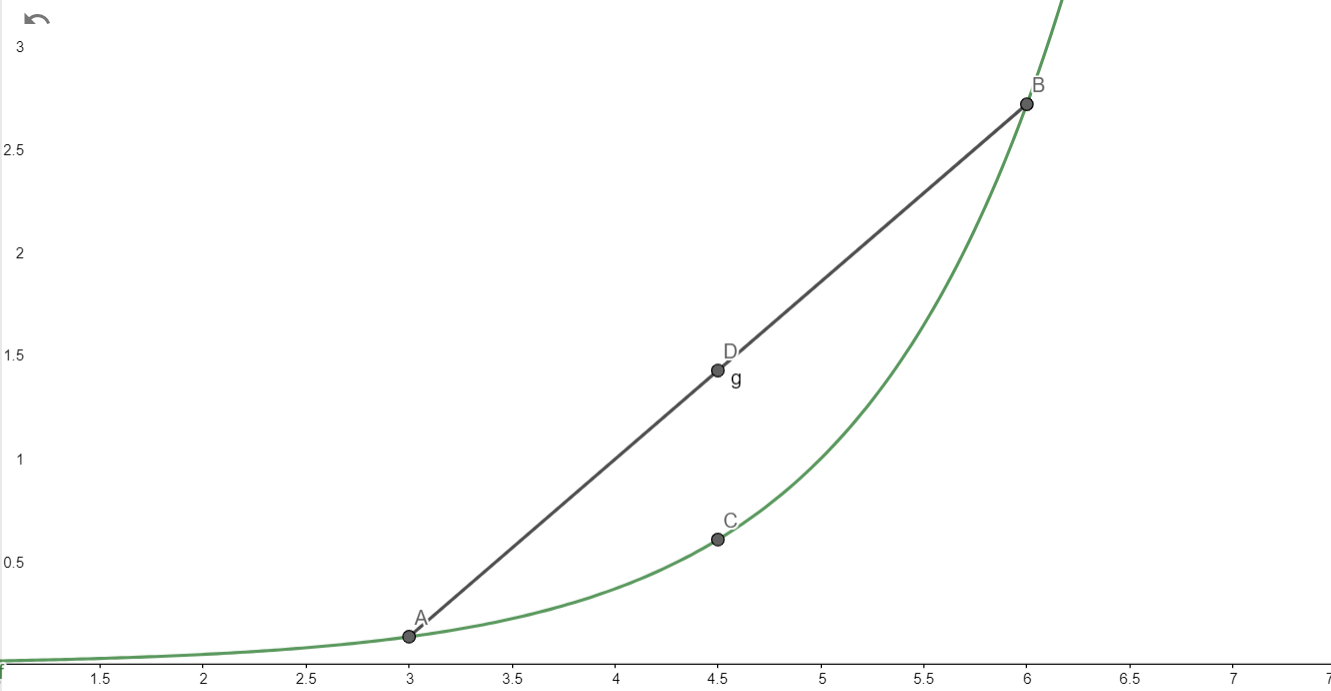
\includegraphics[scale=0.30]{convexidad 2}
\end{center}

En el fondo, lo que decimos es que la proyección del punto sobre la recta siempre está por encima de la imagen cuando nos encontramos en un intervalo de convexidad.

\begin{theo}[Caracterización de la Convexidad]
Sea $f:I\rightarrow\mathbb R$, donde $I$ es un intervalo abierto, una función con dos derivadas en $I$. La función $f$ es convexa en $I$ si y sólo si $\forall x\in I: f''(x)>0$.
\end{theo}
\begin{demo}
\begin{itemize}
\item $\Leftarrow$:

Para poder demostrarlo vamos a demostrar este resultado:
$$f(tx_0+(1-t)x_1)\leq tf(x_0)+(1-t)f(x_1)$$
Fijamos $x_0$ y $x_1$ de $I$ y $t\in (0,1)$. Sea $z=tx_0+(1-t)x_1$ vamos a hacer un desarrollo de Taylor de orden 1 centrado en $z$:
$$f(x)=f(z)+f'(z)(x-z)+\frac{f''(c)}{2}(x-z)^2$$
Luego tenemos que:
$$\begin{cases}f(x_0)=f(z)+f'(z)(x_0-z)+\frac{f''(c_0)}{2}(x_0-z)^2 \\ f(x_1)=f(z)+f'(z)(x_1-z)+\frac{f''(c_1)}{2}(x_1-z)^2\end{cases}$$
En ambos casos el resto de Lagrange es positivo y, en consecuencia, como se cumple que es positivo para todos los $c\in (x_0, z)$ o $c\in (z,x_1)$. Por tanto ahora tenemos:
$$\begin{cases}f(x_0)\geq f(z)+f'(z)(x_0-z) \\ f(x_1)\geq f(z)+f'(z)(x_1-z)\end{cases}\Rightarrow \begin{cases}tf(x_0)\geq tf(z)+tf'(z)(x_0-z) \\ (1-t)f(x_1)\geq (1-t)f(z)+(1-t)f'(z)(x_1-z)\end{cases}\Rightarrow $$
$$\Rightarrow tf(x_0)+(1-t)f(x_1)\geq f(z)+f'(z)(\underbrace{tx_0+(1-t)x_1-z}_{=0})\Rightarrow tf(x_0)+(1-t)f(x_1)\geq f(tx_0+(1-t)x_1)$$

\item $\Rightarrow$:

Supongamos que $f$ es convexa y $a\in I$, lo que vamos a ver es:
$$f''(a)=\lim_{h\rightarrow 0} \frac{f(a+h)-2f(a)+f(a-h)}{h^2}$$
Esto lo asumimos como cierto. Veamos ahora que como $a$ es el punto medio de $a+h$ y $a-h$ para cualquier $h$, entonces se puede expresar como combinación lineal convexa de ambos puntos:
$$a=\frac{1}{2}(a-h)+\frac{1}{2}(a+h)\stackrel{Convexa}{\Rightarrow} f(a)\leq \frac{1}{2}f(a-h)+\frac{1}{2}f(a+h)\Leftrightarrow \frac{1}{2}f(a-h)+\frac{1}{2}f(a+h) - 2f(a) \geq 0\Rightarrow $$
$$\Rightarrow \frac{\frac{1}{2}f(a-h)+\frac{1}{2}f(a+h) - 2f(a)}{h^2}\geq 0\Rightarrow f''(a)=\lim >0$$

Falta solo demostrar la parte que hemos usado de $f''(a)=\lim_{h\rightarrow 0 }\frac{f(a+h)-2f(a)+f(a-h)}{h^2}$. Si definimos $\psi(h) = f(a+h)-2f(a)+f(a-h)$ entonces vemos que es continua y derivable porque las que la componen lo son. Ahora calculamos, aplicando L'Hopital, el límite:
$$\lim_{h\rightarrow 0}\frac{\psi(h)}{h^2}=\lim_{h\rightarrow 0}\frac{f'(a+h)-f'(a-h)}{2h}= \cancel{\lim_{h\rightarrow 0}\frac{f''(a+h)-f''(a-h)}{2}}$$
Pero esto no puede hacerse porque no podemos asumir que la segunda derivada sea continua, en su caso vamos a proceder a hacer esto:
$$\lim_{h\rightarrow 0} \frac{f'(a+h)-f'(a)+f'(a)-f'(a-h)}{2h}= \frac{1}{2}\left(\lim_{h\rightarrow 0}\frac{f'(a+h)-f'(a)}{h}+ \lim_{h\rightarrow 0} \frac{f'(a)-f'(a-h)}{h}\right) = $$
$$=\frac{1}{2}\left(f''(a)+ f''(a)\right)=f''(a)$$
\end{itemize}
\end{demo}

\begin{obs}
La manera intuitiva de ver que este teorema tenía que ser cierto es que $f''(x)>0$ implica que $f'(x)$ es creciente en ese intervalo y vimos que la interpretación geométrica de la derivada era la pendiente de la recta tangente a la curva en un punto. Por tanto, las rectas tangentes van siendo cada vez más pronunciadas y eso es lo que es la idea de convexidad.
\end{obs}

\subsection{Método de Newton para calcular raíces de f(x)}
Si calculamos la recta tangente a la función en un punto cercano a una raíz, vemos que esta corta cerca de la raíz. Si hacemos lo mismo con los sucesivos puntos de corte de cada una de las tangentes, los puntos de corte cada vez se aproximan más a la raíz que buscamos aproximar.
\begin{center}
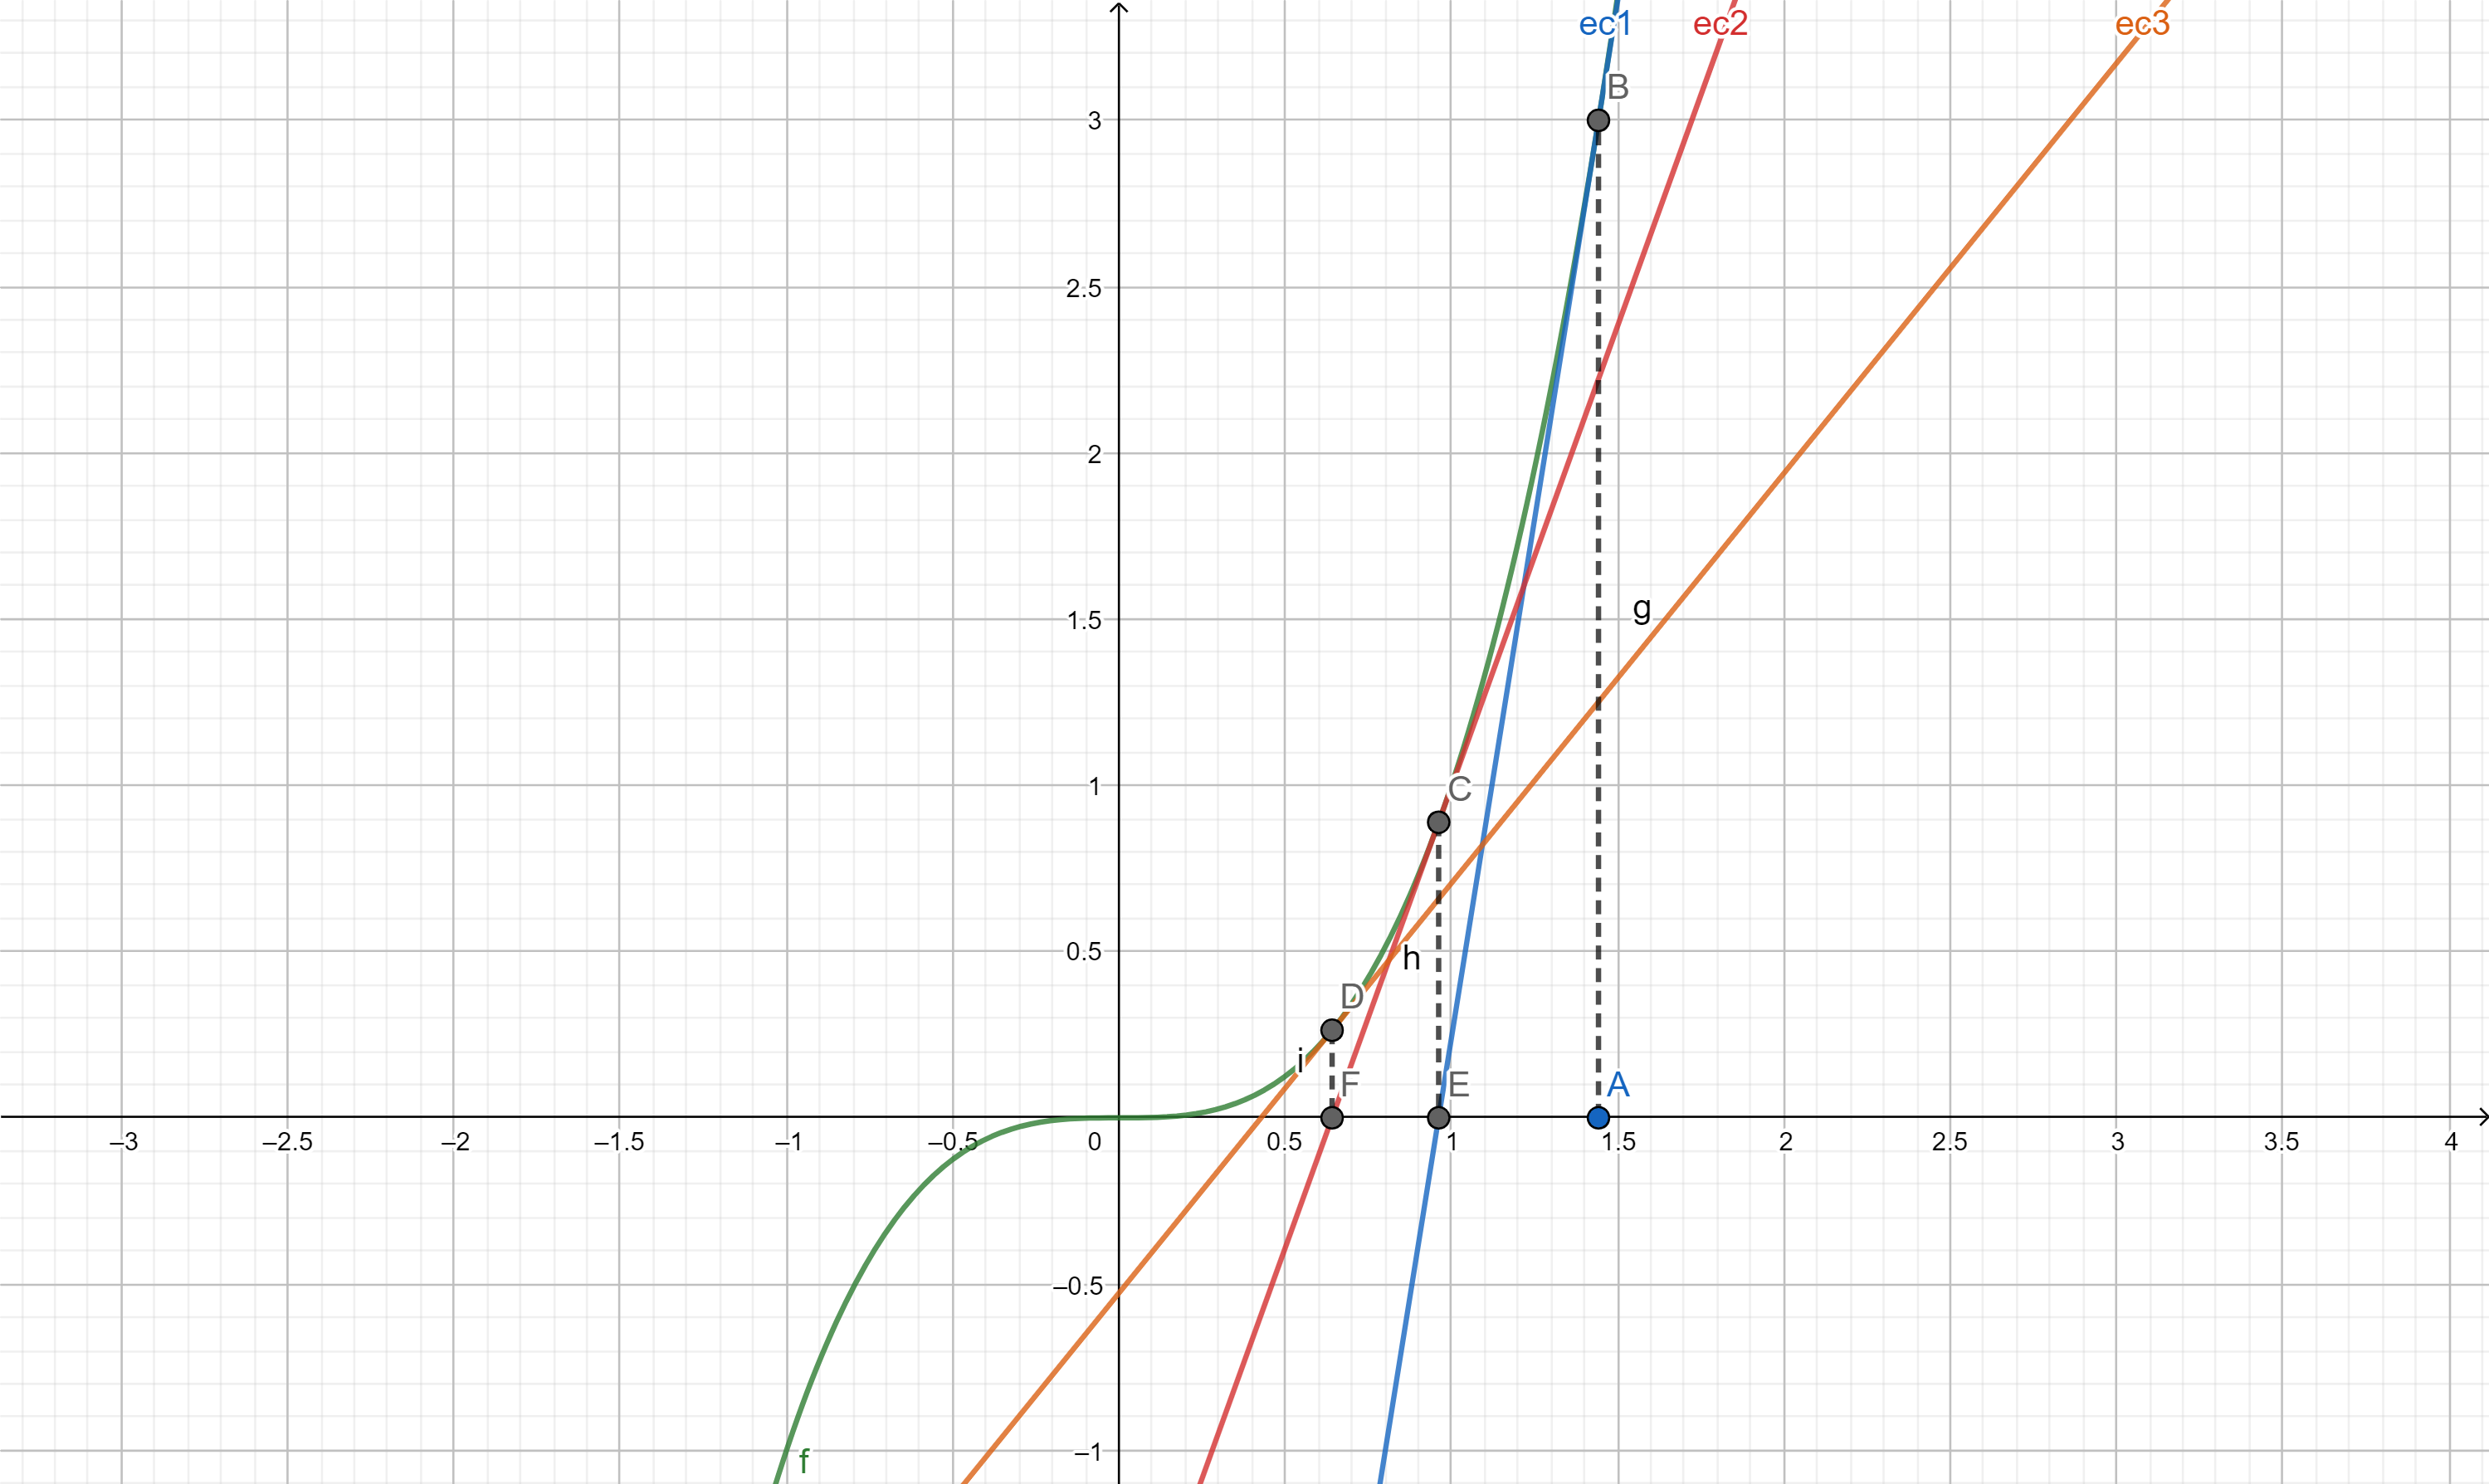
\includegraphics[scale=1.6]{metodo Newton}
\end{center}
Indudablemente, este método puede fallar si no nos encontramos suficientemente cerca de la raíz porque puede ocurrir que uno de los cortes caiga justo en un punto cuya derivada es 0 y en ese caso la recta tangente no cortaría al eje en ningún punto.

Para ver la relación entre un punto y el siguiente, estudiamos la recta tangente: $y-f(x')=f'(x')(x-x')$ y $x''$ es tal que $(x'', 0)$ está en la recta así que:
$$0-f(x')=f'(x')(x''-x')\Leftrightarrow \frac{-f(x')}{f'(x')}=x''-x'$$
Es decir, tenemos una sucesión de puntos para realizar las sucesivas iteraciones del algoritmo y que cada vez están más cerca de la raíz:
$$x_{n+1}=x_n-\frac{f(x_n)}{f'(x_n)}$$

\begin{theo}
Sea $f: [a,b]\rightarrow \mathbb R$ una función que verifica:
\begin{itemize}
\item $f(a)\cdot f(b)<0$ (signos distintos)
\item $|f'(x)|\geq m>0$
\item $\forall x\in [a,b]: |f''(x)|\leq M$
\end{itemize}
entonces podemos afirmar que $\exists r!\in (a,b):f(r)=0\mbox{ y } \exists \delta > 0 : [r-\delta, r+\delta]\subset [a,b]$ tal que:
$$\forall x_0\in [r-\delta, r+\delta]\Rightarrow \begin{cases}\{x_n\}_{n=0}^\infty \subset [r-\delta, r+\delta] \\ |x_{n+1}-r|\leq K\cdot |x_n-r|^2 &\mbox{ tal que } K=\frac{M}{2m} \\ x_n\xrightarrow{n\rightarrow \infty}r \end{cases}$$
\end{theo}
\begin{demo}
Lo primero, por el Teorema de Bolzano se cumple que $\exists r\in (a,b): f(r)=0$, además $f'(x)\neq 0: \forall x\in [a,b]$ por suponer que la derivada es mayor que $m$ y entonces por el Teorema de Rolle, la raíz es única.

Sea $x'\in (a,b)$ vamos a hacer el desarrollo de Taylor centrado en $x'$:
$$f(z)=f(x')+f(x')(z-x')+\frac{f''(c)}{2}(z-x')^2$$
Entonces tenemos ahora que si $z=r$, ocurre que: 
$$0=f(x')+f'(x')(r-x')+\frac{f''(c)}{2}(r-x')^2\Leftrightarrow -\frac{f(x')}{f'(x')}+x'-r=\frac{1}{2}\cdot \frac{f''(c)}{f'(x')}(r-x')^2$$
$$\underbrace{x'-\frac{f(x')}{f'(x')}}_{=x''}-r =\frac{1}{2} \frac{f''(c)}{f'(x')}(x'-r)^2\Rightarrow |x''-r|=\frac{1}{2}\cdot \left|\frac{f''(c)}{f'(x')}\right||x'-r|^2\leq \underbrace{\frac{M}{2m}}_{=K}|x'-r|^2$$
Sea $\delta>0: [r-\delta, r+\delta]\subset (a,b)$ y $K\cdot \delta <1$. Entonces si $x'\in [r-\delta, r+\delta]\Rightarrow |x''-r|\leq K\underbrace{|x'-r|}_{\leq \delta}\cdot |x'-r|\leq |x'-r|$. Lo que quiere decir que la distancia de $x''$ a $r$ es menor que la que había con respecto a $x'$ y, en consecuencia, $x''\in [r-\delta, r+\delta]$.

Y esto me permite ahora definir por inducción la sucesión de manera que:
$$x_0\in [r-\delta, r+\delta]\Rightarrow x_{n+1}=x_n-\frac{f(x_n)}{f'(x_n)}: \{x_n\}_{n=0}^\infty \subset [r-\delta, r+\delta]$$
Y por último veamos que la sucesión converge a la raíz:
$$|x_{n+1}-r|\leq K|x_n-r|^2=K|x_n-r|\cdot |x_n-r|\leq K\delta \cdot |x_n-r|$$
Es fácil ver que como $K\delta<1$ las sucesivas distancias se van haciendo más pequeñas de manera que cada vez está todo más junto, luego:
$$|x_1-r|\leq K\delta |x_0-r|$$
$$|x_2-r|\leq K\delta\cdot |x_1-r|\leq (K\delta)^2 |x_0-r|$$
$$|x_n-r|\leq (K\delta)^n |x_0-r|\Rightarrow x_n-r\xrightarrow{n\rightarrow \infty}0\Rightarrow x_n\xrightarrow{n\rightarrow \infty} r$$

Además la convergencia de esta sucesión es muy rápida, llamemos al error de la aproximación $e_n=|x_n-r|$, luego $e_{n+1}\leq Ke_n^2\Rightarrow Ke_{n+1}\leq (Ke_n)^2$ luego si suponemos que en la primera iteración el error es de $10^{-1}$, tenemos:
$$Ke_1=10^{-1}\Rightarrow Ke_2=10^{-2}\Rightarrow Ke_3=10^{-4}\Rightarrow Ke_4=10^{-8}$$
\end{demo}

\begin{ej}
Veamos por ejemplo el método para calcular la raíz $\sqrt{2}$ de la función $f(x)=x^2-2$.

Es notable que $f(1)<0$ y $f(2)>0$, que $\forall x\in [1,2]: f'(x)\geq 2$ y $f''(x)=2$ luego estamos en las condiciones del Teorema:
$$x_{n+1}=x_n-\frac{f(x_n)}{f'(x_n)}=x_n-\frac{x_n^2-2}{2x_n}=\frac{x_n}{2}+\frac{1}{x_n}$$
Comenzamos con $x_1=1$, entonces $x_2=\frac{3}{2}$, $x_3=\frac{17}{12}$ y así podemos seguir aproximando hasta conseguir el error deseado.
\end{ej}

\chapter{Cálculo Integral}
Si bien la derivación abordaba problemas como las rectas tangentes a funciones, el cálculo de máximos y mínimos y problemas de optimización entre otras cosas, las integrales resuelven un problema fundamental como es el cálculo de áreas, es decir, conocer el área bajo la curva de una función.

Cuando las cosas son rectas, poseemos métodos geométricos (como la triangularización) para poder dividir el problema en otros más pequeños que sí se resolver y luego unir todas las áreas.

\begin{center}
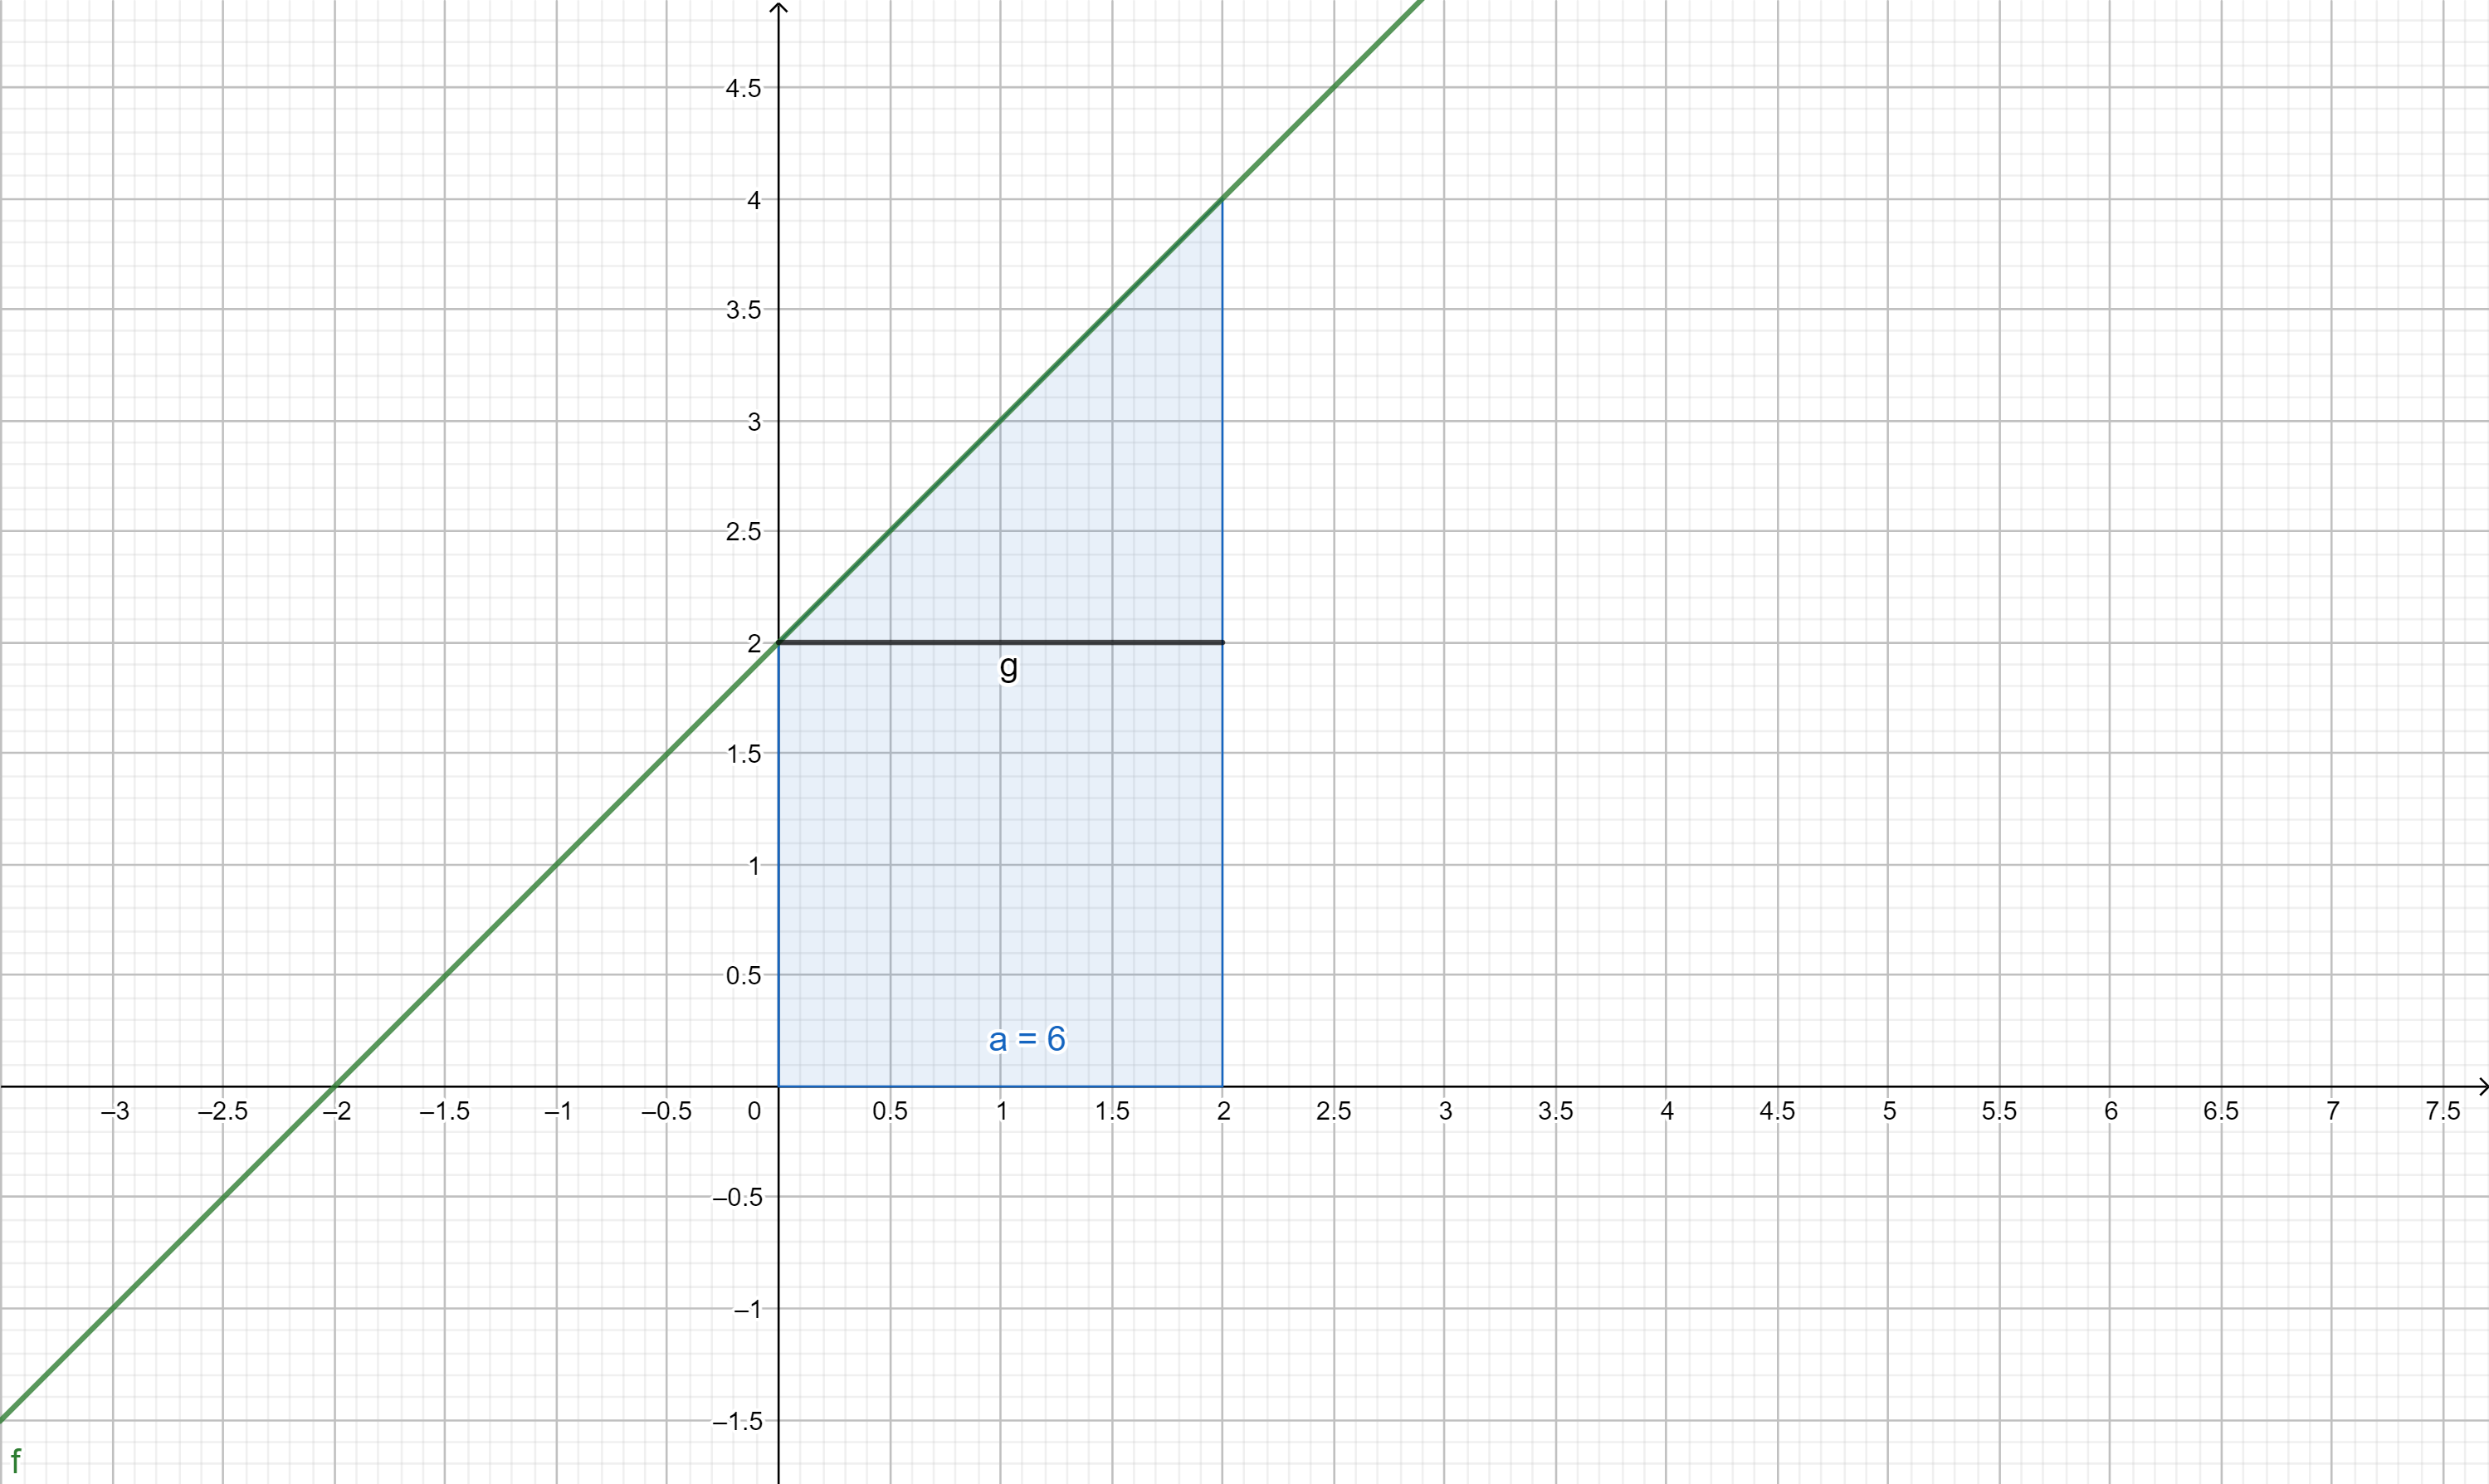
\includegraphics[scale=0.8]{area facil}
\end{center}

El problema viene cuando encontramos funciones que no son rectas, sino que describen curvas y no somos capaces de poder aplicar estos métodos. Una forma de aproximar este tipo de áreas es dividir el eje $x$ en segmentos y hallar el rectángulo de cada uno de los segmentos. Sumándolas todas tenemos una aproximación más o menos buena cuanto en función de la pequeñez de esos segmentos.

\begin{center}
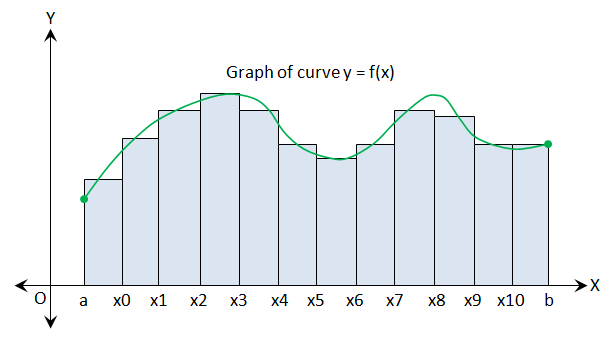
\includegraphics[scale=0.4]{integral de curvas}
\end{center}

Como cada vez que disminuyo la base de los rectángulos, la aproximación es mejor, la suma de las áreas converge a su valor real cuando la longitud del segmento tiende a 0. Dicho concepto representa la idea de dividir en infinitos trozos  para que los rectángulos aproximen lo mejor posible el área bajo la curva.

\section{Teoría de la Integración}
Pasando un poco a la definición más formal, tenemos que definir primero qué es eso de hacer rectángulos y dividir trozos. Lo haremos a través del concepto de partición de un conjunto.
\begin{defi}[Partición y Norma]
Sea $[a,b]\subset \mathbb{R}$ un intervalo, definimos una \textbf{partición} suya como un conjunto de puntos de dicho intervalo que lo dividen en segmentos más pequeños:
$$\wp=\{x_0=a<x_1<x_2<\cdots <x_n=b\}$$
$$DIBUJO$$
Del mismo modo, se define la \textbf{norma de la partición} como  la mayor amplitud entre los subsegmentos generados:
$$||\wp||=\max\{x_i-x_{i-1}\}$$
\end{defi}

\begin{defi}[Particiones Marcadas y Equiespaciadas]
Sea $[a,b]\subset \mathbb{R}$ un intervalo y $\wp$ una partición del mismo, decimos que es una \textbf{partición uniforme o equiespaciada} si y sólo si todos los subsegmentos tienen la misma longitud:
$$\wp=\{x_0=a < x_1< \cdots < x_n=b\}: x_i = a + i \cdot \underbrace{\frac{b-a}{n}}_{=||\wp||}$$
Además, decimos que es \textbf{partición marcada o etiquetada}  y lo denotamos por $\mathring{\wp}$ si y sólo si existe un conjunto de puntos $\forall i = 1, ..., n: \exists! t_i\in [x_{i-1}, x_i]$ (uno por intervalo) a los que llamaremos marcas.
\end{defi}

\begin{defi}[Suma de Riemann]
Sea $f: [a,b]\rightarrow \mathbb R$ y $\mathring{\wp}=\{a=x_0<x_1<\cdots < x_n = b\}: \exists! t_i\in [x_{i-1}, x_i]$ una partición marcada, definimos la \textbf{Suma de Riemann de $f$ en $\mathring{P}$} como:
$$S(f,\mathring{\wp})=\sum_{i=1}^n f(t_i)(x_i-x_{i-1})$$
es decir, es el área formada por los rectángulos cuya base son los segmentos que hemos definido y cuya altura es la imagen de la marca escogida.
\end{defi}

\begin{defi}[Integral de Riemann]
Sea $f:[a,b]\rightarrow \mathbb R$ una función, decimos\footnote{En definitiva, lo que decimos es que si en esa Suma de Riemann, hacemos que $n$ sea muy grande para que la norma sea muy pequeña, entonces su distancia al número $L$ es muy pequeña.} que es \textbf{integrable en el sentido de Riemann} y lo denotamos por $f\in R[a,b]$ si y sólo si $\exists L\in \mathbb R$ de forma que:
$$\forall \varepsilon>0: \exists \delta>0: \forall \mathring{\wp}: ||\wp||<\delta: \left|S(f,\mathring{\wp})-L\right|<\varepsilon$$
Al valor $L\in \mathbb{R}$ mencionado anteriormente lo llamaremos la \textbf{integral de f entre a y b} y lo denotaremos por:
$$L=\int_a^b f(x)\dif{x}$$
Al conjunto de funciones integrables Riemann en el intervalo $[a,b]$ lo denotamos por $R[a,b]$.
\end{defi}

\begin{theo}
Sea $f:[a,b]\rightarrow \mathbb{R}$ una función integrable y $\exists L \in \mathbb R$ su integral, entonces dicha integral es única.
\end{theo}
\begin{demo}
Supongamos que existen dos $L$ y $L'$ que verifican la definición, por lo que:
$$\begin{cases}\varepsilon>0: \exists \delta: ||\mathring{\wp}||<\delta\Rightarrow |S(f,\mathring{\wp})-L|<\varepsilon \\ \varepsilon>0: \exists \delta': ||\mathring{\wp}||<\delta'\Rightarrow |S(f,\mathring{\wp})-L'|<\varepsilon \end{cases}$$
Luego tomando una partición de forma que $||\wp||<\min\{\delta, \delta'\}$ tenemos que:
$$\begin{cases}|S(f,\mathring{\wp})-L|<\varepsilon \\ |S(f,\mathring{\wp})-L'|<\varepsilon\end{cases}\Rightarrow |L-L'|=|L-S(f,\mathring{\wp})+S(f,\mathring{\wp})-L'|\leq |L-S(f,\mathring{\wp})|+|S(f,\mathring{\wp})-L'|<2\varepsilon\Rightarrow L=L'$$
\end{demo}

\begin{ej}
Supongamos que $f(x)=k\in \mathbb R$ definida en $[a,b]$. Tenemos pues que si definimos una partición marcada de la forma que lo hemos estado haciendo antes, entonces:
$$S(f,\mathring{\wp})= \sum_{i=1}^n\underbrace{f(t_i)}_{=k}(x_i-x_{i-1})=k\sum_{i=1}^n(x_i-x_{i-1})=k\cdot (b-a)$$
Con lo cual esta tiene que ser la integral porque si elijo $L=k(b-a)\Rightarrow S(f,\mathring{\wp})-L=0<\varepsilon: \forall \varepsilon$.
\end{ej}

\begin{ej}
Con otro ejemplo, supongamos que $f(x)=x$ definida en $[0,1]$. Vemos que si tomamos la partición de forma que las marcas sean el punto medio $t_i=\frac{x_i+x_{i-1}}{2}$, entonces se tiene que:
$$S(f,\mathring{\wp})=\sum_{i=1}^nf(t_i)(x_i-x_{i-1})=\sum_{i=1}^n t_i(x_i-x_{i-1})=\sum_{i=1}^n \frac{x_i+x_{i-1}}{2}(x_i-x_{i-1})=\frac{1}{2}\sum_{i=1}^n (x_i^2-x_{i-1}^2)=\frac{x_n^2-x_0^2}{2} = \frac{1}{2}$$
Pero en este caso no hemos probado todavía que la integral sea este valor porque hemos impuesto que las marcas sean unas concretas, sin embargo, sí prueba que la integral, de existir, debe ser $L=\frac{1}{2}$ porque como se debe cumplir para todas, para la que hemos hallado este es su valor.

Ahora si escogemos $\mathring{\wp}$ una partición marcada cualquiera vamos a calcular la suma de Riemann y probar que está cerca de $\frac{1}{2}$:
$$S(f,\wp)-\frac{1}{2}= \sum_{i=1}^n f(t_i)(x_{i}-x_{i-1})-\sum_{i=1}^n \frac{x_i-x_{i-1}}{2}(x_i-x_{i-1})=\sum_{i=1}^n \left(t_i- \frac{x_i-x_{i-1}}{2}\right)(x_i-x_{i-1})$$
Tomando ahora valores absolutos:
$$\left|S(f,\wp)-\frac{1}{2}\right| = \left| \sum_{i=1}^n \left(t_i- \frac{x_i-x_{i-1}}{2}\right)(x_i-x_{i-1})\right|\leq \sum_{i=1}^n \left|t_i-\frac{x_i-x_{i-1}}{2}\right|(x_i-x_{i-1})\leq $$
$$\leq \sum_{i=1}^n \delta (x_i-x_{i-1})=\delta \sum_{i=1}^n (x_i-x_{i-1})= \delta$$
Por lo tanto, volviendo a la definición:
$$\delta = \varepsilon >0 \Rightarrow \forall \varepsilon >0: \exists \delta >0: ||\wp||<\delta\Rightarrow |S(f,\wp)-\frac{1}{2}|<\delta =\varepsilon$$
\end{ej}

\subsection{Criterios de Integrabilidad}
\begin{theo}
Sea $g\in R[a,b]$ y $f:[a,b]\rightarrow \mathbb R$ una función que coincide con $g$ excepto en una cantidad finita de puntos que llamaremos $\{c_0, \cdots, c_n\}$, entonces:
$$f\in R[a,b] \mbox{ y } \int_{a}^bf(x)\dif{x}=\int_a^bg(x)\dif{x}$$
\end{theo}
\begin{demo}
La demostración basta hacerla para un punto puesto que luego por inducción podemos extenderlo a $n$ puntos.

Supongamos que $\forall x \in [a,b]\backslash\{c\}: f(x)=g(x)$. Sea $\mathring{\wp}=\{a=x_0< x_1 < \cdots < x_n=b\}: \exists! t_i\in [x_i, x_{i-1}]$ que serán las marcas. Vamos a analizar como puede afectar el punto $c$ a la suma de Riemann, hay dos posibles casos: que $c$ se encuentre en uno de los intervalo o que sea el extremo de uno de los intervalos. En el primer caso solo afecta a uno de los intervalo de la suma de Riemann y en el segundo puede llegar afectar a 2 si fuese marca de ambos intervalos. Entonces poniéndonos en el peor de los casos, que afectase a dos, vemos que:
$$S(f,\mathring{\wp})=\sum_{i=1}^n f(t_i)(x_i-x_{i-1})=$$
Distinguimos los sumandos ``raros'' de los demás:
$$=\sum_{i=1}^{i_0-1}f(t_i)(x_i-x_{i-1})+ f(t_{i_0})(x_{i_0}-x_{i_0-1})+f(t_{i_0+1})(x_{i_0+1}-x_{i_0})+\sum_{i=i_0+2}^n f(t_i)(x_i-x_{i-1})=$$
Como en todos los intervalos menos en los afectados por $c$ la $f$ y la $g$ coinciden, ocurre que $f(t_i)=g(t_i)$ en todos esos intervalos ``normales'', así que podemos escribirlo en función de $S(g,\mathring{\wp})$ pero en los términos ``raros'' tendremos que restar $g(t_\lambda)$ porque lo sumamos en el primer término:
$$=\underbrace{\sum_{i=1}^{n}g(t_i)(x_i-x_{i-1})}_{=S(g,\mathring{\wp})}+ \left(f(t_{i_0})-g(t_{i_0})\right)(x_{i_0}-x_{i_0-1})+\left(f(t_{i_0+1})-g(t_{i_0+1})\right)(x_{i_0+1}-x_{i_0})\Rightarrow $$
Restamos $L=\int_a^b g$ a ambos lados de la igualdad:
$$\Rightarrow S(f,\mathring{\wp})-L = S(g,\mathring{\wp})-L + \left(f(t_{i_0})-g(t_{i_0})\right)(x_{i_0}-x_{i_0-1})+\left(f(t_{i_0+1})-g(t_{i_0+1})\right)(x_{i_0+1}-x_{i_0})\Rightarrow $$
$$\Rightarrow \left|S(f,\mathring{\wp})-L\right| \leq \left|S(g,\mathring{\wp})-L\right| + \left|f(c)-g(c)\right|\cdot ||\mathring{\wp}||+\left|f(c)-g(c)\right|\cdot ||\mathring{\wp}||$$
Entonces, dado $\varepsilon>0: \exists \delta_1>0 : ||\mathring{\wp}||<\delta_1\Rightarrow |S(g,\mathring{\wp})-L|<\frac{\varepsilon}{2}$. Del mismo modo, con el mismo $\varepsilon>0$ escogemos un $\delta_2 = \frac{\varepsilon}{4|f(c)-g(c)|}>0$. En consecuencia, $\delta = \min\{\delta_1, \delta_2\}$ conlleva que:
$$||\mathring{\wp}||<\delta\Rightarrow \left|S(f,\mathring{\wp})-L\right| \leq \frac{\varepsilon}{2}+2|f(c)-g(c)|\cdot \frac{\varepsilon}{4|f(c)-g(c)|}=\frac{\varepsilon}{2}+\frac{\varepsilon}{2}=\varepsilon$$
Así que ya queda demostrado para un único punto.

Después por inducción tenemos que si tenemos $g\in R[a,b]$ y $f\in R[a,b]\backslash\{c_1, c_2\}$, entonces construimos $h\in R[a,b]\backslash\{c_1\}$. Por o probado $\int_a^b g = \int_a^b h= \int_a^b f$. Así que el argumento por inducción se ve claro.
\end{demo}

\begin{theo}
Sea $f\in[a,b]\rightarrow \mathbb R$ la función $f(x)=\begin{cases}\alpha & x\in [a,c) \\ \beta & x\in [c,b]\end{cases}$, entonces $f\in R[a,b]$ y ocurre:
$$\int_a^b f = \alpha (c-a)+\beta(b-c)$$
\end{theo}
\begin{demo}
Sea $\mathring{\wp}$ una partición marcada de forma que $\mathring{\wp} = \{a=x_0 < \cdots <x_n = b\}$. De nuevo el punto $c$ puede quedar en el interior o en uno de los extremos de los intervalos de la partición. Veamos que:
$$S(f,\mathring{\wp}) = \sum_{i=1}^n f(t_i)(x_i-x_{i-1}) = $$
$$=\sum_{i=1}^{i_0-1}f(t_i)(x_i-x_{i-1})+f(t_{i_0})(x_{i_0}-x_{i_0-1})+ f(t_{i_0+1})(x_{i_0+1}-x_{i_0})+\sum_{i=i_0+2}^n f(t_i)(x_i-x_{i-1}) = $$
$$= \sum_{i=1}^{i_0-1}\alpha(x_i-x_{i-1})+\underbrace{f(t_{i_0})(x_{i_0}-x_{i_0-1})+ f(t_{i_0+1})(x_{i_0+1}-x_{i_0})}_{=\varphi}+\sum_{i=i_0+2}^n \beta(x_i-x_{i-1})=$$
$$=\alpha(x_{i_0-1}-a)+\varphi+\beta(b-x_{i_0+1})\Rightarrow $$
Ahora vamos a restar nuestro candidato a integral y vamos a medir esa distancia:
$$\left|S(f,\mathring{\wp})-L \right| =\left|\alpha(x_{i_0-1}-a)+\varphi + \beta(b-x_{i_0+1})-\alpha (c-a)-\beta (b-c)\right| = $$
$$=\left| \alpha \underbrace{(x_{i_0}-c)}_{\leq 2||\mathring{\wp}||}+\beta \underbrace{(c-x_{i_0-1})}_{\leq 2||\mathring{\wp}||} + \varphi\right| \leq \alpha\cdot 2||\mathring{\wp}||+ \beta \cdot 2||\mathring{\wp}|| + \left( |f(t_{i_0})|+|f(t_{i_0-1})| \right)||\mathring{\wp}|| \leq$$
Los términos $\alpha$ y $\beta$ están acotados por el máximo entre ambos y los $f(t_\lambda)$ son o $\alpha$ o $\beta$ por lo que si acotamos los 3 por encima tenemos que:
$$\leq 6 \max\{|\alpha|,|\beta|\}||\wp||$$
Por lo tanto:
$$\forall \varepsilon >0 : \delta = \frac{\varepsilon}{6\max\{|\alpha|, |\beta|\}}: ||\wp||<\delta\Rightarrow \left|S(f,\wp)-L\right|\leq 6 \max\{|\alpha|,|\beta|\}||\wp|| \leq 6 \max\{|\alpha|,|\beta|\} \frac{\varepsilon}{6\max\{|\alpha|, |\beta|\}} = \varepsilon$$
\end{demo}

\begin{obs}
Lo que viene a explicar este teorema, aunque no sea de forma general, es que las discontinuidades de salto no son un impedimento para la integrabilidad.
\end{obs}

\begin{theo}[Acotamiento por integrabilidad]
Toda función $f\in R[a,b]$ es acotada, es decir:
$$\exists M>0:\forall x\in [a,b] :|f(x)|\leq M$$
Luego, las discontinuidades de salto infinito o esenciales impiden la integrabilidad.
\end{theo}
\begin{demo}
Por ser integrable se tiene que:
$$\exists L\in \mathbb R: \forall \varepsilon >0 : \exists \delta >0 : ||\mathring{\wp}||<\delta \Rightarrow |S(f,\mathring{\wp})-L|<\varepsilon$$
Antes de nada, como se cumple para todo $\varepsilon$, vamos a fijar $\varepsilon = 1$ y, en consecuencia, $\delta$ quedará fijo, convirtiéndose ambos en constantes.

Para demostrarlo, vamos a escoger una partición conveniente de forma que nos sea fácil calcular las cosas. Primero, nuestra partición va a cumplir que sea $n\in \mathbb N: ||\mathring{\wp}|| =\frac{b-a}{n}<\delta$ y en consecuencia cada punto de la partición es $x_i=a+i\cdot \frac{b-a }{n}: i=0,1,..., n$. Del mismo modo, dado $x\in [a,b]$ entonces $\exists i_0: x\in [x_{i_0-1}, x_{i_0}]$, y de esta forma vamos a escoger las marcas de la partición de la siguiente forma $\wp_x = \{a=x_0<\cdots < x_n = b\}$ donde $t_i=x_i$ para $i\neq i_0$ pero $t_{i_0}=x$ y de forma que $||\mathring{\wp_x}||=\frac{b-a}{n}<\delta$. Con esta partición veamos que:
$$S(f,\mathring{\wp_x})=\sum_{i=1}^n f(t_i)(x_i-x_{i-1})=\sum_{i\neq i_0} f(x_i)(x_i-x_{i-1}) + f(x)(x_{i_0}-x_{i_0-1})\Rightarrow$$
$$\Rightarrow f(x)=\frac{n}{b-a}\cdot \left[S(f,\wp_x)-\sum_{i\neq i_0} f(t_i)(x_i-x_{i-1})\right]\Rightarrow |f(x)|\leq \frac{n}{b-a}\cdot \left[\left|S(f,\wp_x)\right|+\sum_{i\neq i_0} |f(x_i)|\cdot \frac{b-a}{n}\right] \leq \ast$$
La suma de Rieman se puede acotar porque:
$$\left|S(f,\mathring{\wp_x})\right| = |S(f,\wp_x)-L+L|\leq  \underbrace{|S(f,\wp_x)-L|}_{\varepsilon = 1}+|L|< 1+|L|$$
Con lo cual, si meto el término de $i_0$ de nuevo en el sumatorio, obviamente eso tiene que ser más grande que no meterlo, con lo que la desigualdad queda:
$$\ast \leq \frac{n}{b-a}\left[1 + |L| + \sum_{i=1}^n |f(x_i)|\frac{b-a}{n}\right]=M$$
Es decir, todo lo que queda al final es un único valor constante que no de depende de nada, con lo cual lo podemos llamar $M$ y queda demostrado.
\end{demo}

\begin{theo}[Operaciones con Integrabilidad]
Si $f,g\in R[a,b]$ y $k\in \mathbb R$, entonces:
\begin{enumerate}
\item $kf\in R[a,b]\Rightarrow \int_a^b kf = k\int_a^b f$
\item $f+g\in R[a,b]\Rightarrow \int_a^b (f+g)=\int_a^b f+\int_a^b g$
\item $\forall x\in [a,b]: f(x)\leq g(x)\Rightarrow \int_a^b f \leq \int_a^b g$
\end{enumerate}
\end{theo}
\begin{demo}
\begin{enumerate}
\item Si $\mathring{\wp}$ es una partición marcada entonces ocurre que $S(kf,\wp) = \sum_{i=1}^n(kf)(t_i)(x_i-x_{i-1})=k\sum_{i=1}^n f(t_i)(x_i-x_{i-1})=kS(f,\wp)$

\item Es fácil ver que $S(f+g, \wp)=S(f,\wp)+S(g,\wp)$. A su vez, como $f$ y $g$ son integrables tenemos que:
$$\varepsilon > 0 : \begin{cases}\delta_1>0: ||\wp ||<\delta_1\Rightarrow \left|S(f,\wp)-\int_a^b f\right|<\frac{\varepsilon}{2} \\ \delta_2>0: ||\wp ||<\delta_2\Rightarrow \left|S(g,\wp)-\int_a^b g\right|<\frac{\varepsilon}{2}  \end{cases}$$
Ahora si escogemos $\delta = \min\{\delta_1, \delta_2\}>0$ si $||\wp ||<\delta$ entonces se tiene que:
$$\left| S(f+g,\wp)-\int_a^b f-\int_a^b g \right|=\left|S(f,\wp)+S(g,\wp)-\int_a^b f-\int_a^b g\right| \leq \left|S(f,\wp)-\int_a^b f\right|\left| S(g,\wp)-\int_a^b g\right| <\varepsilon $$

\item También es sencillo ver que $S(f,\mathring{\wp}) \leq S(g,\mathring{\wp})$:
$$\varepsilon > 0 : \begin{cases}\delta_1>0: ||\wp ||<\delta_1\Rightarrow \left|S(f,\wp)-\int_a^b f\right|<\frac{\varepsilon}{2} \\ \delta_2>0: ||\wp ||<\delta_2\Rightarrow \left|S(g,\wp)-\int_a^b g\right|<\frac{\varepsilon}{2}  \end{cases}$$
Ahora si escogemos $\delta = \min\{\delta_1, \delta_2\}>0$ si $||\wp ||<\delta$ entonces se tiene en particular que:
$$\begin{cases} \int_{a}^{b} f -\frac{\varepsilon}{2} < S(f,\mathring{\wp}) < \int_{a}^{b} f + \frac{\varepsilon}{2} \\ \int_{a}^{b} g -\frac{\varepsilon}{2} < S(g,\mathring{\wp}) < \int_{a}^{b} g + \frac{\varepsilon}{2}\end{cases}\Rightarrow  \int_{a}^{b} f -\frac{\varepsilon}{2} < S(f,\mathring{\wp}) \leq S(g,\mathring{\wp}) < \int_{a}^{b} g + \frac{\varepsilon}{2}\Rightarrow $$
$$\Rightarrow \int_{a}^{b}f\leq \int_{a}^{b}g +\varepsilon\Rightarrow \int_{a}^{b}f\leq \int_{a}^{b}g$$
\end{enumerate}
\end{demo}

\begin{defi}[Función Característica]
Sea $A\subset I=[a,b]$, definimos la \textbf{función característica} como:
$$\chi_A(x)=\begin{cases}1 & x\in A \\ 0 & x\notin A\end{cases}$$
\end{defi}

\begin{obs}
Si $c\in (a,b)$, entonces $\chi_{[c,b]}\in R[a,b]$ porque es una función de las que probamos que tenían saltos y eran integrables, además:
$$\int_{a}^{b}\chi_{[c,b]}(x)\dif{x}=b-c$$
\end{obs}

\begin{defi}[Función Escalera]
Sea $I=[a,b]$ y $a=c_0< c_1 <\cdots < c_n=b$, y denotamos por $I_i=[c_{i-1},c_i]$, por tanto, $I=\cup_{i=1}^n I_i$ de forma que $I_i\cap I_j = \emptyset : i\neq j$. De esta forma, definimos una \textbf{función escalera} $\alpha(x)$ como:
$$\alpha(x)=\begin{cases} \alpha_1 & I_1 \\ \alpha_2 & I_2 \\ \vdots \\ \alpha_n & I_n \end{cases}$$
\begin{center}
\includegraphics[scale=0.50]{función escalera}
\end{center}
De hecho podemos escribir:
$$\alpha(x)=\sum_{i=0}^{n}\alpha_i\chi_{I_i}(x) = \int_{a}^{b}\alpha = \sum_{i=1}^{n}\alpha_i (c_i-c_{i-1})$$
\end{defi}

\begin{obs}
Y además ocurre que $\alpha(x)\in R[a,b]$ porque las funciones características son integrables, los $\alpha$ son constantes y además a pesar de que puede haber intervalos con ambos extremos abiertos o no cerrados por ambos lados, como cuando una función se diferencia de otra sigue siendo integrable con la misma integral, entonces aún así sigue siendo integrable.
\end{obs}

\begin{theo}[Criterio de Cauchy]
Sea $f:[a,b]\rightarrow \mathbb R$, la función $f\in R[a,b]$ si y sólo si:
$$\forall \varepsilon > 0: \exists \eta > 0 : ||\mathring{\wp}|| \mbox{ y } ||\mathring{\mathcal{Q}}|| < \eta \Rightarrow \left| S(f,\mathring{\wp})- S(f, \mathring{\mathcal{Q}})\right| < \varepsilon $$
\end{theo}
\begin{demo}
\begin{itemize}
\item $\Rightarrow$:
$$f\in R[a,b]\Rightarrow \varepsilon >0 : \begin{cases}\exists \delta >0: ||\mathring{\wp}|| < \delta \Rightarrow |S(f,\mathring{\wp})-L| < \frac{\varepsilon}{2} \\ \exists \delta'>0: ||\mathring{\mathcal{Q}}||< \delta': |S(f, \mathring{\mathcal{Q}})-L|< \frac{\varepsilon}{2} \end{cases}\Rightarrow$$
Tomando como $\eta = \min\{\delta, \delta'\}$:
$$\Rightarrow |S(f,\mathring{\wp})-S(f,\mathring{\mathcal{Q}})|= |S(f,\mathring{\wp})-L+L-S(f,\mathring{\mathcal{Q}})| \leq \frac{\varepsilon}{2}+\frac{\varepsilon}{2}$$

\item $\Leftarrow$:

En primer lugar, necesitamos un candidato a $L$, por lo que vamos a obtenerlo. Sea $\mathring{\wp_n}$ una partición marcada equiespaciada con $t_i=x_i$. Ocurre que $||\mathring{\wp_n}||=\frac{b-a}{n}$. Sea $s_n=S(f,\mathring{\wp_n})\Rightarrow \{s_n\}_{n=1}^\infty \subset \mathbb R$ una sucesión y vamos a probar que esta sucesión es de Cauchy porque el posible límite al que converja, tendrá que ser necesariamente nuestro candidato a integral:

Dado $\varepsilon >0$ podemos escoger un $n_0\in \mathbb N$ de forma que $n_0> \frac{b-a}{\eta}$ siendo $\eta$ el asociado a $\varepsilon$, con lo cual de esta forma la norma de $P_{n_0}$ va a ser menor que $\eta$ y para cualquier $P_{n}$ con $n\geq n_0$ también se va a verificar esto. Por tanto, puedo afirmar:
$$n,m\geq n_0\Rightarrow \frac{b-a}{n}, \frac{b-a}{m}<\eta\Rightarrow ||\mathring{\wp_n}||,||\mathring{\wp_m}||<\eta\Rightarrow |s_n-s_m|=|S(f,\mathring{\wp_n})-S(f,\mathring{\wp_m})|<\varepsilon$$
Lo que implica que la sucesión $\{s_n\}$ es de Cauchy, así que $\exists L = \lim_{n\rightarrow \infty} s_n$ y este debe ser mi candidato a integral.

Es decir, que por un lado ocurre que:
$$\varepsilon > 0 : \exists \eta >0: |S(f,\mathring{\wp})-S(f, \mathring{\mathcal{Q}})|<\frac{\varepsilon}{2}$$

Por otro lado, sea $n_0\in \mathbb N: \frac{b-a}{n_0}<\eta$. La partición concreta que habíamos definido $\mathring{\wp_{n_0}}$ verifica que $||\mathring{\wp_{n_0}}||<\frac{b-a}{n_0}<\eta$. Además como $\lim_{n\rightarrow \infty} s_n = L\Rightarrow \exists n_1\in \mathbb N: \forall n \geq n_1 \Rightarrow  |s_n-L|<\frac{\varepsilon}{2}$. Con lo cual tomando el mayor de los dos se tiene que $\tilde{n}=\max\{n_0,n_1\}$ ocurre:
$$||\wp_{\tilde{n}}||<\eta$$
Y también se verifica:
$$|s_{\tilde{n}}-L|<\frac{\varepsilon}{2}$$
Con lo cual ocurre que:
$$|S(f,\wp)-L|=|S(f,\wp)-S(f,\wp_{\tilde{n}})+S(f, \wp_{\tilde{n}})-L|\leq |S(f,\wp )- S(f,\wp_{\tilde{n}})|+|s_n-L|\leq \frac{\varepsilon}{2} + \frac{\varepsilon}{2} = \varepsilon$$
\end{itemize}
\end{demo}

\begin{obs}
Este teorema aporta un criterio muy potente \textbf{que no requiere de tener candidato a integral} para poder afirmar que es integrable o no.
\end{obs}

\begin{theo}[Criterio del Sandwich]
Sea $f:[a,b]\rightarrow \mathbb R$, la función $f\in R[a,b]$ si y sólo si:
$$\forall \varepsilon >0 : \exists \alpha_\varepsilon, \omega_\varepsilon: [a,b]\rightarrow \mathbb R : \alpha_\varepsilon, \omega_\varepsilon \in R[a,b]: \alpha_\varepsilon \leq f(x)\leq \omega_\varepsilon (x): \forall x\in [a,b]$$
Además, ambas funciones auxiliares deben verificar que:
$$\int_{a}^{b} \omega_\varepsilon(x)-\alpha_\varepsilon(x) \dif{x} < \varepsilon$$
\begin{center}
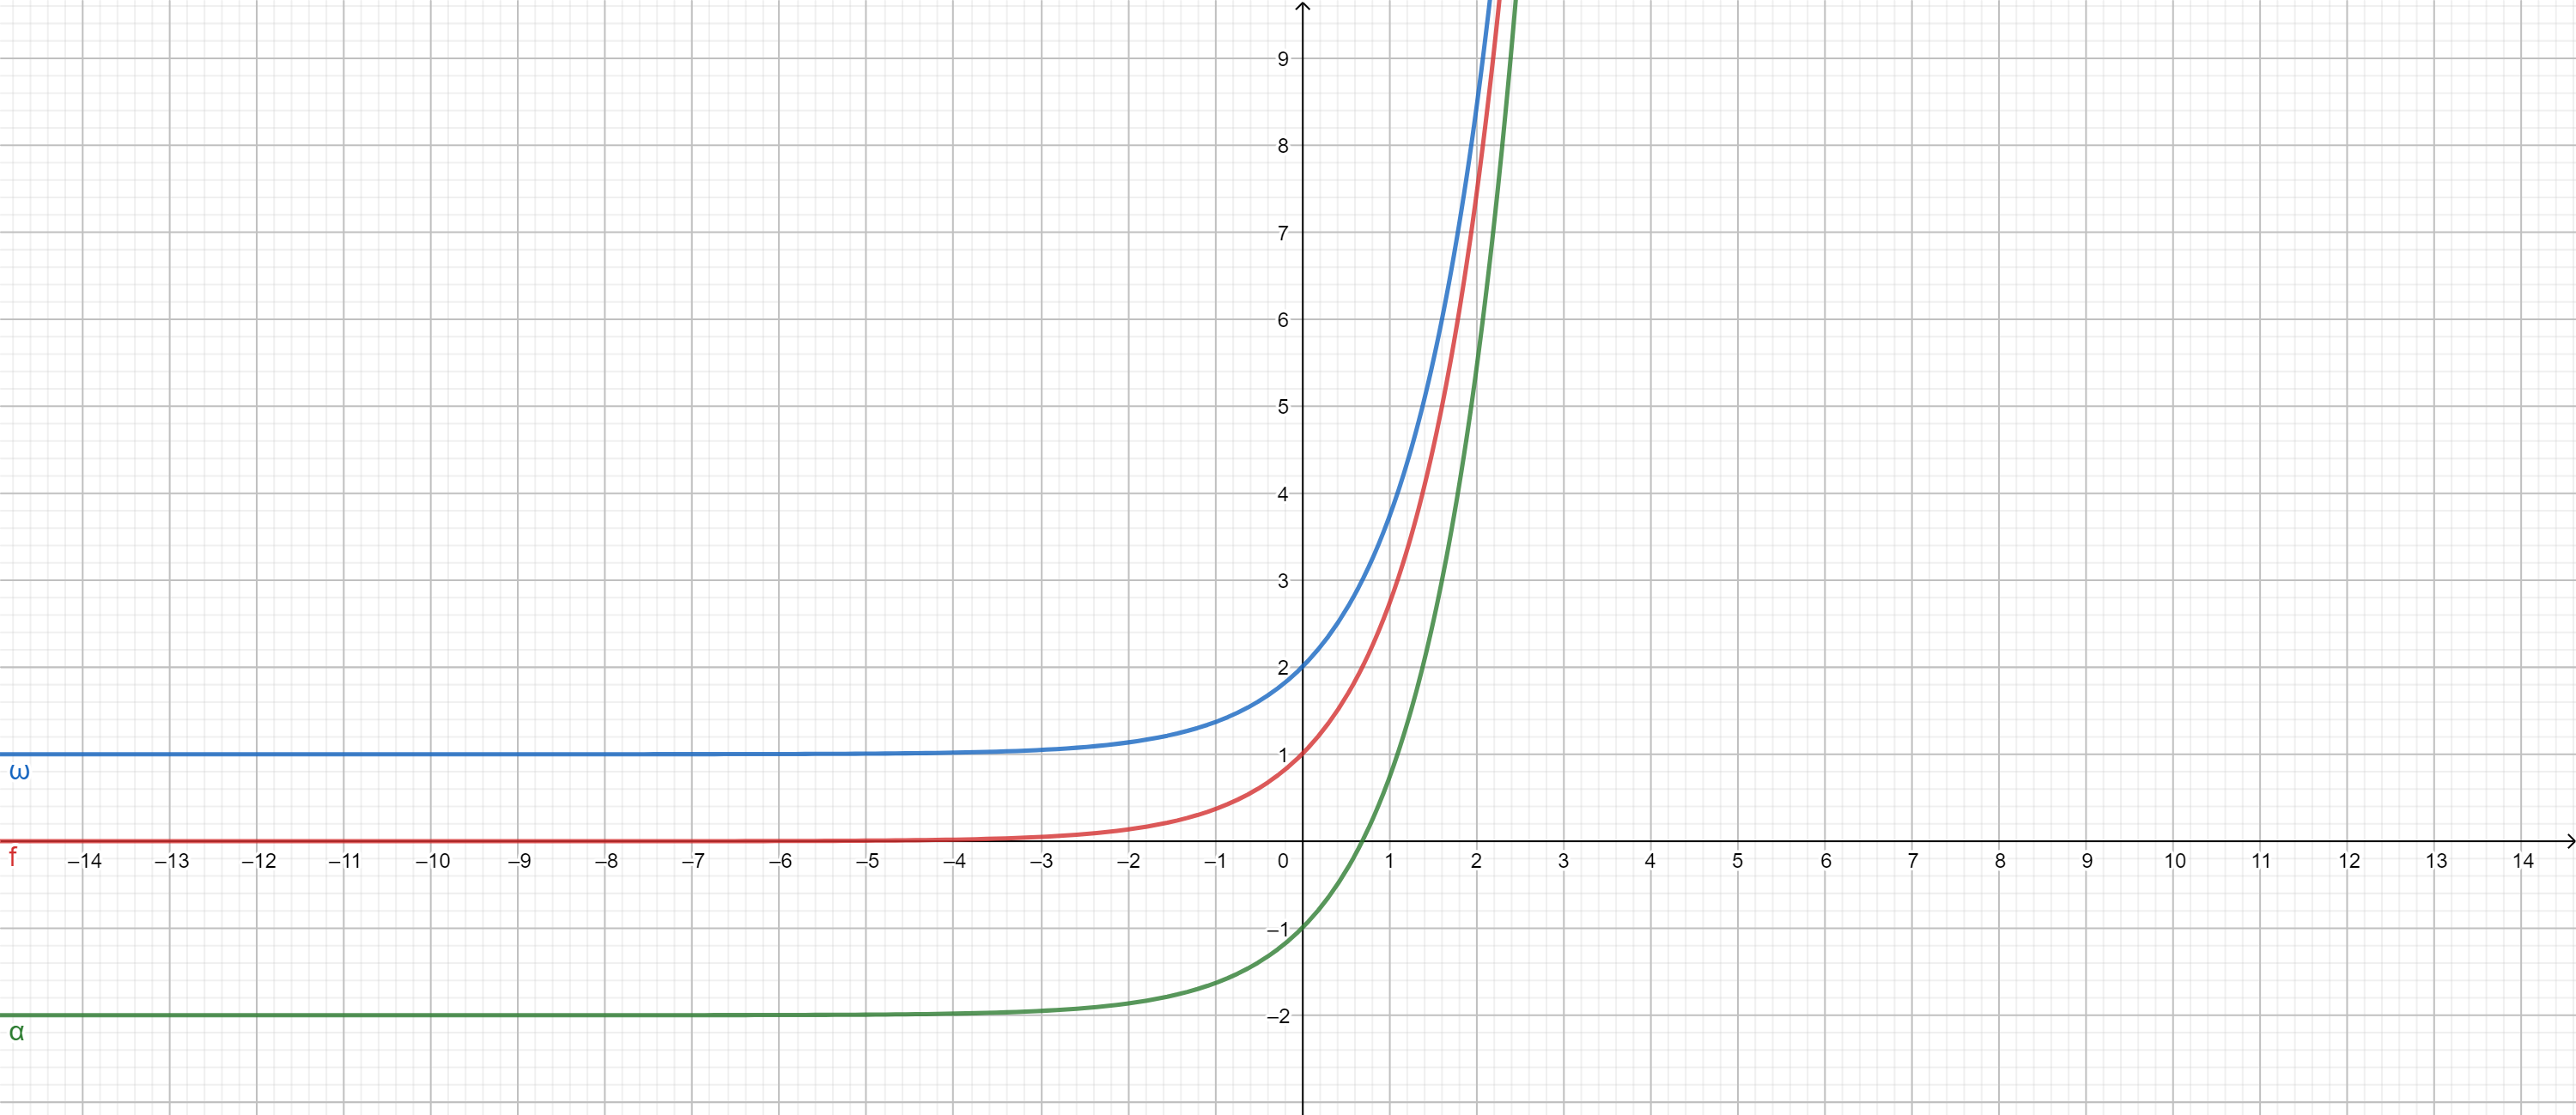
\includegraphics[scale=0.45]{criterio sandwich para integrales}
\end{center}
\end{theo}
\begin{demo}
\begin{itemize}
\item $\Rightarrow $:

Si $f\in R[a,b]$ basta con tomar $\alpha_\varepsilon = \omega_\varepsilon = f$ para cualquier $\varepsilon$ por lo que se deduce que trivialmente se verifican las premisas

\item $\Leftarrow$:

Tenemos que $\alpha_\varepsilon\in R[a,b]$, entonces:
$$\varepsilon > 0 :\exists \delta_1 >0: ||\mathring{\wp}||<\delta_1\Rightarrow \left|S(f,\mathring{\wp})-\int_{a}^{b}\alpha_\varepsilon \right|<\varepsilon$$

Del mismo modo, como $\omega_\varepsilon\in R[a,b]$, entonces:
$$\varepsilon >0: \exists \delta_2>0 : ||\mathring{\wp}||<\delta_2\Rightarrow \left|S(f,\mathring{\wp})- \int_{a}^{b}\omega_\varepsilon \right| <\varepsilon$$

Denominamos $\eta = \min\{\delta_1, \delta_2\} >0$ y definimos $\mathring{\wp}$ y $\mathring{\mathcal{Q}}$ dos particiones marcadas de forma que $||\mathring{\wp}||,||\mathring{\mathcal{Q}}||<\eta$ se tiene que por un lado:
$$\int_{a}^{b}\alpha_\varepsilon -\varepsilon < S(\alpha_\varepsilon, \mathring{\wp}) < \int_{a}^{b}\alpha_\varepsilon + \varepsilon$$
Y por otro:
$$\int_{a}^{b}\omega\varepsilon -\varepsilon < S(\omega\varepsilon, \mathring{\wp}) < \int_{a}^{b}\omega_\varepsilon + \varepsilon$$
Asímismo, como $\alpha_\varepsilon < f(x)< \omega_\varepsilon$, entonces:
$$S(\alpha_\varepsilon, \mathring{\wp}) < S(f,\mathring{\wp}) < S(\omega_\varepsilon, \mathring{\wp})\Rightarrow \int_{a}^{b}\alpha_\varepsilon - \varepsilon < S(\alpha_\varepsilon, \mathring{\wp}) < S(f,\mathring{\wp}) < S(\omega_\varepsilon, \mathring{\wp}) < \int_{a}^{b}\omega_\varepsilon + \varepsilon$$
De la misma forma se pueden aplicar estos razonamientos a $\mathring{\mathcal{Q}}$ por lo que se tiene que:
$$\int_{a}^{b}\alpha_\varepsilon - \varepsilon < S(\alpha_\varepsilon, \mathring{\mathcal{Q}}) < S(f,\mathring{\mathcal{Q}}) < S(\omega_\varepsilon, \mathring{\mathcal{Q}}) < \int_{a}^{b}\omega_\varepsilon + \varepsilon$$
Por tanto ahora por el Criterio de Cauchy se tiene que si multiplicamos una de las desigualdades por -1 y después sumamos obtenemos:
$$-\int_{a}^{b}(\omega_\varepsilon - \alpha_\varepsilon)-2\varepsilon \leq S(f,\mathring{\wp})- S(f,\mathring{\mathcal{Q}})\leq \int_{a}^{b}(\omega_\varepsilon - \alpha_\varepsilon) + 2\varepsilon$$
Y como por hipótesis teníamos la relación entre la integral de la diferencia de $\alpha_\varepsilon$ y $\omega_\varepsilon$ entonces:
$$-3 \varepsilon\leq -\int_{a}^{b}(\omega_\varepsilon - \alpha_\varepsilon)-2\varepsilon \leq S(f,\mathring{\wp})- S(f,\mathring{\mathcal{Q}})\leq \int_{a}^{b}\omega_\varepsilon - \alpha_\varepsilon + 2\varepsilon < 3\varepsilon\Rightarrow$$
$$\Rightarrow \left|S(f,\mathring{\wp})- S(f,\mathring{\mathcal{Q}})\right| < 3\varepsilon$$
Luego por el Criterio de Cauchy es integrable
\end{itemize}
\end{demo}

\begin{obs}
Para poder demostrar la integrabilidad de funciones más patológicas se suele usar este teorema y una muy buena práctica para poder acotarla como queramos puede ser utilizar las funciones escalera que definimos para que cuadre todo como queramos.
\end{obs}

\begin{prop}[Criterios de no integrabilidad]
Son unas condiciones suficientes para afirmar que una función no es integrable:
\begin{itemize}
\item Si existe una sucesión de particiones marcadas $\mathring{\wp_n}$ de forma que $||\mathring{\wp_n}||\xrightarrow{n\rightarrow \infty} 0 $ y $S(f,\mathring{\wp_n})\cancel{\longrightarrow} l$, entonces $f\notin R[a,b]$.

\item Si existen dos sucesiones de particiones marcadas $\mathring{\wp_n}$ y $\mathring{\mathcal{Q}_n}$ de forma que $S(f,\mathring{\wp})\xrightarrow{n\rightarrow \infty} L_1$ y $S(f,\mathring{\mathcal{Q}})\xrightarrow{n\rightarrow \infty} L_2$ pero $L_1\neq L_2$, entonces $f\notin R[a,b]$.
\end{itemize}
\end{prop}
\begin{demo}
\begin{itemize}
\item Por el criterio de Cauchy, la sucesión de número reales $s_n = S(f,\mathring{\wp_n})$ es una sucesión de Cauchy y por lo tanto es convergente y la afirmación que hemos dado contradice dichos postulados.
\item Del mismo modo, se contradicen las hipótesis del Criterio de Cauchy ya que la sucesión no puede tener dos límites distintos por la unicidad del límite.
\end{itemize}
\end{demo}

\begin{theo}
Dadas las siguientes definiciones:
\begin{itemize}
\item $R[a,b]$ como el conjunto de funciones integrables de Riemann.
\item $C[a,b]$ como el conjunto de funciones continuas.
\item $C^{1}[a,b]$ como el conjunto de funciones continuas y cuya derivada también es continua.
\item $C^{k}[a,b]$ como el conjunto de funciones continuas y cuyas derivadas hasta la $k-$-ésima son continuas.
\item $B[a,b]$ como al conjunto de funciones acotadas.
\item $M[a,b]$ como el conjunto de funciones monótonas.
\end{itemize}
Las funciones continuas también son integrables:
$$C[a,b]\subset R[a,b]$$
Las funciones monótonas también son integrables:
$$M[a,b]\subset R[a,b]$$
\end{theo}
\begin{demo}
Sea $f\in C[a,b]$, como $[a,b]$ es cerrado y acotado, entonces $f$ es uniformemente continua en $[a,b]$, luego:
$$\forall \varepsilon > 0: \exists \delta> 0: |x-y|<\delta\Rightarrow |f(x)-f(y)|<\varepsilon$$
Por lo tanto, si escogemos $\frac{\varepsilon}{b-a}$ entonces:
$$\exists \delta : |x-y|<\delta \Rightarrow |f(x)-f(y)|<\frac{\varepsilon}{b-a}$$
Podemos ahora escoger $n_0\in \mathbb N: \frac{b-a}{n_0}<\delta$ y con ese número vamos a hacer una partición uniforme en la que cada punto de la partición viene definido por: $c_i = a+ i \frac{b-a}{n_0}$ con $i = 0, 1, \cdots , n_0$.

Ahora, dado un $[c_{i-1}, c_i]$ vamos a denotar:
$$\begin{cases} f_i = \min\{ f(x): x\in [c_{i-1},c_i]\} \\ f^i = \max\{f(x): x\in [c_{i-1},c_i]\}\end{cases}$$
Por tanto si $x\in [c_{i-1},c_i]$, se tiene que $f_i\leq f(x)\leq f^i$ por definición y existen ambos valores porque por ser continuas se alcanza el máximo y el mínimo.

FALTA EXPLICACIÓN CON DIBUJO

De este modo, escogemos\footnote{Partimos esta función en dos trozos para asegurarnos de que los intervalos donde escogemos las cosas sean disjuntos y de este modo no halla problemas (por eso distinguimos el último)}
$$\alpha_\varepsilon = \begin{cases} f_i & x\in [c_{i-1},c_i): i = 0,1,\cdots , n_0-1 \\ f_{n_0}  & x\in[c_{n_0-1},c_{n_0}] \end{cases}$$
Y de forma análoga tomamos:
$$\omega_\varepsilon = \begin{cases} f^{i} & x\in [c_{i-1},c_i): i = 0,1,\cdots , n_0-1 \\ f^{n_0}  & x\in[c_{n_0-1},c_{n_0}] \end{cases}$$
Estas dos funcione son del tipo que hemos definido como ``función escalera'' por lo que ya sabemos que son integrables.

No es difícil ver que por como están construidas, ambas funciones anteriores verifican que: $\forall x\in[a,b]: \alpha_\varepsilon (x)\leq f(x)\leq \omega_\varepsilon$, solo falta ver que la integral de la diferencia es pequeña para que quede demostrado por el Teorema del Sandwich:
$$\int_{a}^{b}\alpha_\varepsilon(x) \dif{x} = \sum_{i = 1}^{n_0} f_i\cdot (c_i-c_{i-1})$$
$$\int_{a}^{b}\omega_\varepsilon(x) \dif{x} = \sum_{i = 1}^{n_0} f^i\cdot (c_i-c_{i-1})$$
$$\int_{a}^{b} \omega_\varepsilon - \alpha_\varepsilon = \sum_{i = 1}^{n_0} (f^i-f_i)(c_i-c_{i-1})$$
Como cada $f_i$ es el máximo valor que toma la función en algún punto del intervalo, puedo expresarlo como $f(u_i)$, es decir, el valor de la función en ese punto y con $f_i$ ocurre de modo análogo:
$$f^i = \max\{f(x): x\in [c_{i-1},c_{i}]\} =  f(u_i) \mbox{ para cierto } u_i\in [c_{i-1},c_{i}]$$
$$f_i = \min\{f(x): x\in [c_{i-1}, c_{i}]\} = f(v_i)\mbox{ para cierto } v_i\in [c_{i-1},c_{i}]$$
Luego ocurre con ambos que:
$$f^i-f_i = |f^i - f_i| = \left|f(u_i)- f(v_i)\right| \stackrel{|u_i-v_i|\leq \frac{b-a}{n_0}<\delta}{<} \frac{\varepsilon}{b-a}: \forall i = 1, 2,\cdots , n_0 $$
Eso ocurre así porque como es uniformemente continua, si $|x-y|<\delta\Rightarrow |f(x)-f(y)|<\varepsilon$.

En consecuencia, se tiene que:
$$\int_{a}^{b} \omega_\varepsilon - \alpha_\varepsilon = \sum_{i = 1}^{n_0} (f^i-f_i)(c_i-c_{i-1}) \leq \frac{\varepsilon}{b-a}\underbrace{\sum_{ i = 1}^{n_0} (c_i-c_{i-1})}_{=b-a} = \varepsilon$$

Demostración de que las monótonas también los son:

Sea $f$ monótona creciente (el caso decreciente es análogo), es decir, $x\leq y\Rightarrow f(x)\leq f(y)$, definimos la partición uniforme $\mathring{\wp} =\{a = c_0 < c_1 < \cdots < c_n = b\}$.

De este modo, construimos de nuevo:
$$\alpha_\varepsilon = \begin{cases} f(c_{i-1}) & x\in [c_{i-1}, c_i): i=1,..., n_0-1 \\ f(c_{n_0-1}) & x\in [c_{n_0-1}, c_{n_0}]\end{cases}$$
$$\omega_\varepsilon = \begin{cases} f(c_{i}) & x\in [c_{i-1}, c_i): i=1,..., n_0-1 \\ f(c_{n_0}) & x\in [c_{n_0-1}, c_{n_0}]\end{cases}$$
Es decir, en este caso estamos tomando siempre el valor de la función en el punto de la derecha o de la izquierda en cada una de cada uno de los intervalos.

Se verifica trivialmente entonces se cumple que $\forall x\in [a,b]: \alpha(x)\leq f(x)\leq \omega(x)$. Vemos entonces de nuevo, la integral de la diferencia:
$$\int_{a}^{b}\alpha_\varepsilon(x) \dif{x} = \sum_{i = 1}^{n_0} f(c_{i-1})\cdot (c_i-c_{i-1}) = \frac{b-a}{n_0} \cdot (f(c_0)+\cdots + f(c_{n_0-1}))$$
$$\int_{a}^{b}\omega_\varepsilon(x) \dif{x} = \sum_{i = 1}^{n_0} f(c_i)\cdot (c_i-c_{i-1}) = \frac{b-a}{n_0} \cdot (f(c_1)+\cdots + f(c_{n_0}))$$
$$\int_{a}^{b} \omega_\varepsilon - \alpha_\varepsilon = \frac{b-a}{n_0}(f(c_0)+f(c_{n_0})) = \frac{b-a}{n_0}\cdot (f(b)-f(a))$$
Con lo cual como esa diferencia es constante y ese valor es menor que delta, puedo tomar un delta lo suficientemente pequeño como para que no importe esa constante.
\end{demo}

\begin{obs}
Hemos visto que $R[a,b]\subset B[a,b]$, del mismo modo ocurre que $C^k[a,b]\subset C^{1}[a,b]\subset C[a,b]$.
\end{obs}

Hemos visto que las funciones continuas son integrables y las que no lo son, en función del número y tipo de discontinuidades que posean pueden serlo o no. Este criterio otorga una herramienta muy potente para poder caracterizar una función integrable Rieman.

El concepto de medida es complejo y bastante extenso por lo que no ahondaremos mucho en él. A priori para nosotros, la medida de un intervalo $(a,b)$ es el real $b-a$, pero lo que realmente nos interesa es la noción de medida de un conjunto, concretamente la medida nula de un conjunto, es decir, cuando decimos que un conjunto ``no mide nada''. 

\begin{defi}[Conjunto de Medida Nula]
Un conjunto $A\subset \mathbb R$ se dice que es de medida nula si se tiene que:
$$\forall \varepsilon > 0, \exists \mbox{cantidad numerable de intervalos }(a_k,b_k):\forall k = 1,2,\cdots: \begin{cases} A \displaystyle \subset  \displaystyle\bigcup^\infty_{k=1}(a_k,b_k) \\ \displaystyle \sum_{k=1}^{\infty} (b_k - a_k) < \varepsilon\end{cases}$$
\end{defi}

\begin{obs}
En base a esta definición podemos detectar los siguientes conjuntos que poseen medida nula:
\begin{itemize}
\item \textbf{Un punto} posee medida nula

$$\{a\}\subset \{a-\frac{\varepsilon}{2}, a +\frac{\varepsilon}{2}\}\Rightarrow medida(\{a\})\leq medida\left(a-\frac{\varepsilon}{2}, a +\frac{\varepsilon}{2}\right) = \varepsilon$$

\item Una \textbf{cantidad finita de puntos} posee medida nula
$$A = \{a_1, a_2,...,a_n\}\Rightarrow A \subset \bigcup^N_{i=1} \left(a_i - \frac{\varepsilon}{2N}, a_i + \frac{\varepsilon}{2N}\right)$$
$$\sum_{1}^{N} \frac{\varepsilon}{N} = \varepsilon$$

\item Una \textbf{cantidad numerable de puntos} posee medida nula

Supongamos que tenemos una cantidad numerable de puntos $\{a_i\}_{i=1}^\infty$. Sea $\varepsilon >0$, entonces podemos meter cada punto en un intervalo que sea $I_i=\left(a_i-\frac{\varepsilon}{2^{i+1}}, a_i + \frac{\varepsilon}{2^{i+1}}\right)$ cuya medida es concretamente $\frac{\varepsilon}{2^i}$.

De este modo se verifica que:
$$\bigcup^\infty_{i=1} a_i \subset \bigcup^\infty_{i=1} I_i$$
$$\sum_{i=1}^{\infty} \frac{\varepsilon}{2^i} = \varepsilon \left(\frac{1}{2} + \frac{1}{2^2} + \ldots\right) = \varepsilon $$
\end{itemize}
\end{obs}

\begin{theo}[de Lebesque de Integración]
Sea $f:[a,b]\rightarrow \mathbb R$ una función acotada y $D(f)$ el conjunto de puntos de discontinuidad de la función, entonces:
$$f\in R[a,b]\Leftrightarrow D(f) \mbox{ es de medida nula}$$
\end{theo}

\begin{prop}[Operaciones con Medida Nula]
\begin{itemize}
\item Si $D\subset C$ y $C$ es de medida nula, entonces $D$ es de medida nula.
\item Si tenemos $C_1, ..., C_n$ una cantidad finita de conjuntos de medida nula, entonces:
$$\bigcup_{i =1}^{n} C_i\mbox{ es de medida nula}$$
\item Si tenemos una cantidad numerable de conjuntos de medida nula, entonces la medida de la unión de todos es nula.
$$\{C_n\}_{n=1}^\infty\mbox{ de medida nula }\Rightarrow \bigcup_{n=1}^{\infty} C_n \mbox{ es de medida nula}$$
\end{itemize}
\end{prop}

\begin{prop}[Integrabilidad de la composición]
Sea $f:[a,b]\rightarrow \mathbb R$ una función $f\in R[a,b]$ y $\varphi: [c,d]\rightarrow \mathbb R$ continua que verifica $f[a,b]\subset[c,d]$, entonces la función $\varphi \circ f: [a,b]\rightarrow \mathbb R$ verifica $\varphi\circ f \in R[a,b]$.
\end{prop}
\begin{demo}
Si $f$ es continua en $c$, como $\varphi$ es continua, $\varphi\circ f$ es continua en $c$. Dicho de otro modo, la composición solo puede ser discontinua donde lo es $f$:
$$[a,b]\setminus D_f \subset [a,b]\setminus D_{\varphi \circ f} \Leftrightarrow D_{\varphi \circ f} \subset D_f$$
Por tanto, al ser $f\in R[a,b]$, $D_f$ es de medida nula y, en consecuencia, $D_{\varphi\circ f}$ es de medida nula. Si demostramos que es acotada, por el criterio de Lebesque entonces es integrable. Ver que es acotada es sencillo, puesto que $f\in R[a,b]$ es acotada  por ser integrable y $\varphi$ es también es acotada por ser continua, por tanto, la composición de ambas si que está acotada.
\end{demo}

\begin{ej}
Supongamos que $f\in R[a,b]$:
\begin{itemize}
\item ¿$|f(x)|\in R[a,b]$ es integrable?

La respuesta es que sí porque es la función $f$ compuesta con la función $g(x)=|x|$ que sabemos que es continua.

\item ¿$f^a(x)$ donde $a\in \mathbb R$ es integrable?

La respuesta vuelve a ser afirmativa por ser la exponencial continua

\item ¿$f,g\in R[a,b]$ $f\cdot g$ es integrable?

Sí, porque $f+g\in R[a,b]$, del mismo modo $(f+g)^2\in R[a,b]$ y en consecuencia sabemos que $\frac{1}{4}(f+g)^2-\frac{1}{4}(f-g)^2 = f\cdot g\in R[a,b]$

\item ¿La parte positiva $f^+(x)=\varphi(f(x))$ donde $\varphi(x)=\begin{cases} x & x>0 \\ 0 & x\leq 0\end{cases}$?

Por supuesto que sí porque $\varphi$ es una función continua.

\item ¿La función valor máximo $M(x)=\max\{f(x),g(x)\}$ que denotamos por $M(x)=\frac{f+g}{2}+\frac{|f-g|}{2}$?

Sí lo es porque la suma es integrable y la diferencia también que junto con el valor absoluto ya hemos dicho que sí.
\end{itemize}
\end{ej}

\subsubsection{Aditividad de la Integral}
\begin{prop}[Aditividad de la Integral]
Sea $[a,b]$ un intervalo y $c\in [a,b]$, entonces:
$$f \in \mathcal{R}[a,b]\Leftrightarrow f|_{[a,c]} \in \mathcal{R} [a,c] \mbox{ y } f|_{[c,b]} \in \mathcal{R} [c,b]$$
Además, la integral es aditiva:
$$\int_{a}^{b} f = \int_{a}^{c} f + \int_{c}^{b} f$$
\end{prop}
\begin{demo}
\begin{itemize}
\item $\Rightarrow$:

Supongamos que $f\in R[a,b]$, entonces se tiene que por el Criterio de Cauchy:
$$\forall \varepsilon >0:  \exists \eta > 0 : \forall \mathring{P}, \mathring{Q}:  ||\mathring{P} || , ||\mathring{Q} || < \eta \Rightarrow |S(f,\mathring{P}) - S(f,\mathring{Q})| < \varepsilon $$ 

Vamos a definir dos particiones en el trozo que nos interesa
$$\varepsilon > 0: \mbox{sea }\eta > 0\mbox{ el de }[a,b] \mbox{ y sean }\mathring{P}_1, \mathring{Q}_1\mbox{ de }[a,c]: ||\mathring{P}_1 || , ||\mathring{Q}_1 || < \eta$$
y vamos a definir una única complementaria en el otro trozo
$$\mathring{R} = \{c = r_0 < \cdots < r_n = b\}\mbox{de }[c,b]: t_i \in [r_{i-1}, r_i]$$
De forma que uniendo la complementaria con una de las dos que hemos construido se tenga una partición del segmento total:
$$\begin{cases} \mathring{P_1}\cup \mathring{R} = \mathring{P} \\ \mathring{Q_1}\cup \mathring{R} \cup \mathring{Q} \end{cases}\Rightarrow ||\mathring{P}||, ||\mathring{Q}||<\eta$$

Por un lado tenemos entonces que si nos referimos a la suma de Riemann del conjunto:
$$S(f,\mathring{P}) = S(f,\mathring{P}_1) + S(f,\mathring{R})$$
$$S(f,\mathring{Q}) = S(f,\mathring{Q}_1) + S(f,\mathring{R})$$
Por tanto, como la función es integrable en el intervalo completo al ser iguales ambas cosas, la diferencia de ambas particiones de uno de los intervalos también es menor que $\varepsilon$:
$$|S(f,\dot{P}_1) - S(f,\dot{Q}_1)|= |S(f,\mathring{P}_1) + S(f,\mathring{R}) - S(f,\mathring{Q}_1) - S(f,\mathring{R})| = |S(f,\mathring{P}) - S(f,\mathring{Q})| < \varepsilon$$

\item $\Leftarrow$: 

LA DEJA PARA NOSOTROS.
\end{itemize}
\end{demo}

\begin{prop}
\begin{enumerate}
\item Sea $f\in R[a,b]$ y $a<c<d<b$, entonces $f\in R[c,d]$ y la integral verifica:
$$\int_{c}^{d} f = \int_{a}^{d} f - \int_{a}^{c} f$$

\item Sea $\mathring{P} = \{a = c_0 < \cdots < c_n = b\}$ partición en el intervalo $[a,b]$, entonces:
$$\int_{a}^{b} f = \sum_{i = 1}^{n} \left(\int_{c_{i-1}}^{c_i} f\right)$$

\item Sea $f\in R[a,b]$ y $\alpha,\beta\in [a,b]: \alpha < \beta$, entonces:
$$\int_{\beta}^{\alpha} f {=} - \int_{\alpha}^{\beta} f$$
\item La integral en un punto es nula:
$$\int_{\alpha}^{\alpha} f = 0$$
\end{enumerate}
\end{prop}
\begin{demo}
\begin{enumerate}
\item Por el Teorema anterior podemos demostrar que $f\in R[a,d]$, escogiendo ahora un punto intermedio entre $a$ y $d$ que llamaremos $c$, por el Teorema anterior tenemos de nuevo que $f\in R[c,d]$.

\item Lo tenemos demostrado para uno solo, por lo que podemos aplicar inducción para extenderlo al número \textbf{finito} de veces que queramos.

\item Por definición

\item Trivial
\end{enumerate}
\end{demo}

\begin{theo}
Sea $f\in R[a,b]$ y $\alpha,\beta,\gamma\in [a,b]$ cualesquiera\footnote{Es notable destacar que no hemos impuesto ningún tipo de orden entre estos número para realizar dicha afirmación.}, entonces:
$$\int_{\alpha}^{\beta} f+ \int_{\beta}^{\gamma} f = \int_{\alpha}^{\gamma} f$$
\end{theo}
\begin{demo}
Este resultado que acabamos de ver es equivalente a decir:
$$\int_{\alpha}^{\beta} f+ \int_{\beta}^{\gamma} f + \int_{\gamma}^{\alpha} f = 0$$
Por lo que vamos a tratar de demostrar esto

Denotamos por $L(\alpha,\beta,\gamma) = \int_{\alpha}^{\beta} f+ \int_{\beta}^{\gamma} f + \int_{\gamma}^{\alpha} f$ y vamos a distinguir casos:
\begin{itemize}
\item Si alguna de las parejas coincide, es decir, $\alpha = \beta$ o $\alpha = \gamma$ o $\beta = \gamma$, entonces este resultado es trivial.

\item Si los tres son distintos y remarcamos que NO sabemos el orden:
$$L(\alpha , \beta , \gamma) = L(\beta , \gamma , \alpha) = L(\gamma , \alpha , \beta)$$
Como estas permutaciones son las mismas, vamos a estudiar las otras 3 posibles permutaciones distintas:
$$L(\beta , \alpha , \gamma) = \int^\alpha_\beta f + \int^\gamma_\alpha f +  \int^\beta_\gamma = - \int^\beta_\alpha f - \int^\alpha_\gamma f - \int^\gamma_\beta f = - \int^\beta_\alpha f - \int^\gamma_\beta f - \int^\alpha_\gamma f   =  -L(\alpha , \beta , \gamma)$$

Pero de nuevo, si realizo permutaciones circulares sobre este resultado, entonces ocurre que:
$$L(\beta , \alpha , \gamma) = L(\alpha , \gamma , \beta) = L(\gamma , \beta , \alpha) $$
Es decir, que tres coinciden y las otras tres también coinciden y unas son las otras pero cambiando el signo, por tanto, si demostramos que una de ellas es 0, todas lo serán.
$$L(\beta , \alpha , \gamma) = L(\beta , \gamma , \alpha) = L(\gamma , \alpha , \beta) = - L(\beta , \alpha , \gamma) = - L(\alpha , \gamma , \beta) = - L(\gamma , \beta , \alpha) $$
Aunque no sabemos el orden, en alguna de las permutaciones se tendrá el orden que poseen los números elegido y esa demostración ya hemos visto que es cierta, por tanto, siendo uno 0, todos los demás son 0.
$$\alpha < \beta < \gamma \Rightarrow L(\alpha < \beta < \gamma ) = 0\Rightarrow L(\beta , \alpha , \gamma) = \cdots  = - L(\gamma , \beta , \alpha) = 0$$
\end{itemize}
\end{demo}

\subsection{Teorema Fundamental del Cálculo}
La integrabilidad permite determinar si merece la pena gastar el tiempo en calcular o no una integral, pero ¿quién es la integral? En ocasiones, el cálculo de este valor por medio de la definición se vuelve sumamente complejo y no es práctico a la hora de llevarlo a cabo.

Una de las claves del desarrollo matemático moderno ha sido el enunciado de este Teorema porque es la llave que conecta la derivación con la integración y que otorga un pilar sobre el que apoyarse para poder calcular la integral de infinitud de funciones de forma ``sencilla''.

\begin{theo}[Regla de Barrow]
Sea $f\in R[a,b]$, supongamos que $\exists F: [a,b]\rightarrow\mathbb R$ continua en $[a,b]$ y derivable en $(a,b)$ de forma que $\forall x\in \mathbb R: F'(x) = f(x)$, entonces se tiene que:
$$\int_{a}^{b} f(x) \dif{x} = F(b)-F(a)$$
\end{theo}
\begin{demo}
Sea $\mathcal{P} = \{x_0 = a < \cdots < x_n = b\}$ una partición uniforme de $[a,b]$ de forma que $x_i = a + \frac{i}{n} (b-a), i=1,...,n$. Antes de escoger las marcas veamos que:
$$F \in \mathcal{C}[x_{i-1},x_i]\mbox{ derivable en }(x_{i-1},x_i)$$
Por el Teorema del Valor medio tenemos que:
$$\exists c_i \in (x_{i-1},x_1): \frac{F(x_i)-F(x_{i-1})}{x_i - x_{i-1}} = F'(c_i)= f(c_i)$$
Y justamente estas van a ser las marcas de nuestra partición:
$$\mathring{\mathcal{P}}_n = \{a=x_0 < x_1 <...<x_n = b:  t_i = c_i\}$$
En consecuencia, al calcular la suma de Riemann tenemos que:
$$S(f, \mathring{\mathcal{P}}_n)= \sum^n_{i=1} \underbrace{f(c_i)(x_i - x_{i-1})}_{F(x_i)-F(x_{i-1})} = \sum^n_{i=1} \left( F(x_i)-F(x_{i-1}) \right) = F(x_1)- F(x_0) + F(x_2) - F(x_1) + ... + F(x_n)-F(x_{n-1}) =$$
$$= F(x_n) - F(x_0) = F(b) - F(a)$$
Pero como $f \in \mathcal{R}[a,b]$, entonces:
$$\lim_{x \to \infty}S(f, \mathring{\mathcal{P}}_n) = \int^b_a f\Rightarrow \int^b_a f = F(b) - F(a)$$
Porque como $S(f,\mathring{\mathcal{P}_n}) = F(b)-F(a)$ es fijo, entonces al converger a la integral, necesariamente el valor constante es la integral.
\end{demo}

\begin{coro}
Sea $f\in R[a,b]$ y supongamos que $\exists F\in C[a,b]: F'(x) = f(x):\forall x\in [a,b]\setminus E$ donde $E$ es un conjunto finito de puntos, entonces:
$$\int_{a}^{b}f= F(b)- F(a)$$
Es decir, que tras extraer una cantidad finita de puntos sigue siendo cierta la regla de Barrow y la integral es la misma.
\end{coro}
\begin{demo}
Aplicamos la regla de Barrow en $[c_{i-1},c_{i}]: i = 1,2,..., n+1$:

Se puede aplicar esto porque $F$ es continua  y entonces lo es en cada pequeño intervalo. Además como coincide en todos los puntos dentro de ese pequeño intervalo tenemos: $F \in \mathcal{C}[c_i , c_{i-1}]:  F'(x)=f(x): \forall x \in (c_i , c_{i-1})$, luego podemos decir que:
$$\int_{c_{i-1}}^{c_i} f = F(c_i) - F(c_{i-1})$$
Por la aditividad de la integral podemos decir que:
$$\int_{a}^{b} f = \sum_{i=1}^{n+1} \int_{c_{i-1}}^{c_i} f = \sum_{i=1}^{n+1} F(c_i) - F(c_{i-1})= F(c_{n+1}) - F(c_0)  = F(b) - F(a)$$
\end{demo}

\begin{defi}[Integral Indefinida]
Sea $f\in R[a,b]$, definimos la \textbf{integral indefinida con base $a$} como la función $F:[a,b]\rightarrow \mathbb R$ definida por:
$$F(z)=\int_{a}^{z} f$$
\end{defi}

\begin{theo}
Sea $f\in R[a,b]$ y denotando por $F$ su integral indefinida de base $a$, entonces $F\in C[a,b]$ y $F$ es Lipschizt\footnote{Suelen denotarse por $C^{0,1}[a,b]$} con constante\footnote{Este supremo existe porque por ser integrable sabemos que está acotada y por tanto posee supremo.} de Lipschizt:
$$M=  \sup\{|f(x)|\}: x\in [a,b]$$
Además, el ser Lipschiztiana implica:
$$|F(z)-F(w)|\leq M |z-w|: z,w\in [a,b]$$
\end{theo}
\begin{demo}
Sean $z,w\in [a,b]$ dos puntos distintos, supongamos en primer lugar que $a\leq w<z\leq b$, entonces:
$$\begin{cases} F(z)= \int_{a}^{z} f \\ F(w) = \int_{a}^{w} f \end{cases}\Rightarrow F(z)-F(w) = \int_{a}^{z} f -\int_{a}^{w} f = \int_{a}^{z} f +\int_{w}^{a} f = \int_{w}^{z} f$$
Entonces:
$$|F(z)-F(w)| = \left|\int_{w}^{z} f \right|$$
Pero como sabemos que la función $f$ está acotada por ser integrable:
$$-M \leq f(x) \leq M \Rightarrow$$
Y además por la monotonía de la integral:
$$\underbrace{\int_{w}^{z} -M}_{-M(z-w)} \leq \int_{w}^{z} f\leq \underbrace{\int_{w}^{z} M}_{M(z-w)}$$
Luego:
$$|F(z)-F(w)| = \left|\int_{w}^{z} f \right| \leq M|z-w| $$
Ahora si suponemos que $a\leq z<w\leq b$ el razonamiento es completamente simétrico cambiando los roles de $z$ y $w$ en lo que hemos hecho antes, por tanto, lo que queda es que:
$$|F(z)-F(w)| \leq M|z-w| $$

Pero esto es lo mismo que lo de antes, por lo que queda porbado que $F$ es una función Lipstchiziana y por tanto $F\in C[a,b]$.
\end{demo}

\begin{theo}[Fundamental del Cálculo]
Sea $f\in R[a,b]$ continua en $c\in [a,b]$, entonces la función $F$ es derivable en $c$ y además:
$$F'(c) = f(c)$$
\end{theo}
\begin{demo}
Sabemos que $f$ es continua en $c$, lo que quiere decir que:
$$\forall \varepsilon > 0, \exists \delta > 0: \mbox{si }  \underset {x \in [a,b]}{|x-c|<\delta} \Rightarrow |f(x) - f(c)|<\varepsilon  \Leftrightarrow
 f(c)-\varepsilon < f(x)<f(c)+ \varepsilon$$
Para probar que $F$ es derivable y que la derivada en $c$ es $f(c)$, vamos a demostrar que:
$$|z-c|<\delta \Rightarrow \left| \frac{F(z) - F(c)}{z-c} - f(c) \right| < \varepsilon: $$
Veamos que:
$$F(z) - F(c) =  \int_{a}^{z} f - \int_{a}^{c} f = \int_{c}^{z} f$$

Vamos a suponer en primer lugar que $c<z<c+\delta$, como $f(c)-\varepsilon < f(x)<f(c)+ \varepsilon$ y la integral conserva estas desigualdades tenemos que:
$$(f(c) - \varepsilon)(z-c) = \int_{c}^{z} (f(c)-\varepsilon) < \underbrace{\int_{c}^{z} f(x)\dif{x}}_{F(z) - F(c)} < \int_{c}^{z} (f(c)+\varepsilon) = (f(c) + \varepsilon)(z-c) \Rightarrow  $$
$$\Rightarrow f(c) - \varepsilon < \frac{F(z) - F(c)}{z-c} < f(c) + \varepsilon \Rightarrow - \varepsilon < \frac{F(z) - F(c)}{z-c} - f(c) < + \varepsilon \Leftrightarrow$$
$$\Leftrightarrow \left| \frac{F(z) - F(c)}{z-c} - f(c) \right| < \varepsilon: c < z < c+\delta$$
Y el razonamiento para $c-\delta < z <c$ es completamente análogo y queda demostrado por tanto que la derivada de la integral es la función de la que partíamos.
\end{demo}

\begin{obs}
Entre las consecuencias más importantes de este teorema tenemos que:
$$F(z) = \int_{a}^{z} f\Rightarrow \frac{d}{dz}\left(\int_{a}^{z} f\right) (c) = f(c)$$
Además si $f\in C[a,b]$, entonces $F$ es derivable en $[a,b]$ y se tiene que $F'(z) = f(z)$ para todo $z$ en el intervalo y por eso podemos afirmar que:
$$\frac{d}{dz} \int_{a}^{z} f = f(z)$$
Es decir, que derivada de la función integral es la propia función por lo que son operaciones inversas.
\end{obs}

\section{Cálculo de Integrales}
A pesar de que durante todo el capítulo hemos estado definiendo y matizando el concepto de integral y sentando las bases para diferenciar que funciones son integrables y cuáles no, aún no hemos definido herramientas o procedimientos para calcular dicha integral. Esta sección va dedicada precisamente al cálculo numérico de las mismas y a dar criterios de convergencia para las impropias. 

\subsection{Métodos de integración}
Vamos a ver las principales técnicas más sencillas para calcular integrales cuando la integración no es directa, esto es, cuando conocemos directamente la primitiva de la función a integrar.

\begin{theo}[Cambio de Variable]
Sean $f:I\rightarrow \mathbb R$ tal que $f\in C^0(I)$, $\varphi: J\rightarrow \mathbb R$ tal que $\varphi\in C^1(J)$ y de modo que $\varphi(J)\subset I$ y $\alpha,\beta\in J$, entonces:
$$\int_{\alpha}^{\beta} f(\varphi(t))\cdot \varphi'(t)\dif{t} = \int_{\varphi(\alpha)}^{\varphi(\beta)} f(x)\dif{x}$$
\end{theo}
\begin{demo}
Lo primero de todo, es sencillo ver que lo que estamos diciendo está bien definido porque el producto de estas funciones es continuo por las características que tienen y hemos demostrado que las funciones continuas son integrables.

Definimos la función $F(u)=\int_{\varphi(\alpha)}^{u} f(x)\dif{x}: \forall u \in I$, de este modo sabemos que $F'(u)=f(u)$ con lo cual, $F$ es una primitiva de $f$ porque es la integral indefinida de base $\varphi(\alpha)$ tal y como la denotamos.

Consideramos ahora esta función:
$$H(t)=F(\varphi(t))=\int_{\varphi(\alpha)}^{\varphi(t)} f(x)\dif{x}: \forall t\in J$$
De este modo vemos que por la Regla de la Cadena:
$$H'(t)=F'(\varphi(t))\cdot \varphi'(t)= f(\varphi(t))\varphi'(t)$$

Si empleamos la Regla de Barrow, entonces:

$$\int_{\alpha}^{\beta} f(\varphi(t)) \varphi ' (t) \dif{t} = H (\beta) - H(\alpha) = F(\varphi(\beta)) - \underbrace{F(\varphi(\alpha))}_{= 0} =  \int_{\varphi (\alpha)}^{\varphi (\beta)} f(x) \dif{x}$$
\end{demo}

\begin{ej}
En la práctica, este tipo de resultado se usa del siguiente modo. Supongamos que queremos calcular:
$$\int_{0}^{2} 2tsen(t^2)\dif{t}$$
Consideramos:
$$\begin{cases} \varphi(t)=t^2 \\ \alpha = 0, \ \beta = 2 \\
f(x)=sen(x)\end{cases}$$
Por tanto por el Teorema de Cambio de Variable tenemos que:
$$\int_{0}^{2} 2tsen(t^2)\dif{t} = \int_{0}^{4} sen(x)\dif{x} = cos(0)-cos(4)= 1-cos(4)$$

También es útil para el cálculo de primitivas de funciones. Por ejemplo, supongamos que queremos calcular la primitiva de
$$f(t)=t\cdot e^{t^2}$$
No existe una única primitiva, por lo que podemos denotar la familia de todas estas como:
$$\int f(x)\dif{x}$$
Entonces para calcular esta primitiva, basta con aplicar el cambio de variable visto considerando que $ t^2 = x \Rightarrow 2t\dif{t}=\dif{x}$ se tiene:
$$\int t e^{t^2} \dif{t}  = \int e^x \frac{1}{2} \dif{x} = \frac{1}{2} e^x + C \Rightarrow F(t)=\frac{1}{2}e^{t^2} + C$$
\end{ej}

\begin{theo}[Integración por partes]
Sean $F,G\in C^1(I,\mathbb R)$, $f=F'$ y $g=G'$, entonces  para $\alpha,\beta\in I$ se tiene que:
$$\int_{\alpha}^{\beta} f(x)G(x)\dif{x} = F(\beta)G(\beta) - F(\alpha)G(\alpha)-\int_{\alpha}^{\beta} F(x)g(x)\dif{x}$$
\end{theo}
\begin{demo}
Vamos a considerar la función $H(x)=F(x)G(x)$, es sencillo ver que por la Regla del Producto tenemos que:
$$H'(x)=F'(x)G(x)+F(x)G'(x)$$
De este modo, la integral en ambos lados debe ser la misma, es decir:
$$\int_{\alpha}^{\beta} H'(x) \dif{x}= \int_{\alpha}^{\beta} f(x)G(x)\dif{x} + \int_{\alpha}^{\beta} F(x)g(x)\dif{x}$$
Por un lado tenemos que:
$$\int_{\alpha}^{\beta}H'(x)\dif{x} = H(\beta)-H(\alpha) = \left[FG\right]_\alpha^\beta$$
Con lo cual despejando $\displaystyle \int_{\alpha}^{\beta} f(x)G(x)\dif{x}$:
$$\int_{\alpha}^{\beta} f(x)G(x)\dif{x} = [FG]^\beta_\alpha - \int_{\alpha}^{\beta} F(x)g(x)\dif{x}\Rightarrow \int_{\alpha}^{\beta} F'(x)G(x)\dif{x} = [FG]^\beta_\alpha - \int_{\alpha}^{\beta} F(x)G'(x)\dif{x}$$
Lo más representativo es que esta igualdad es aprovechable por ambos lados puesto que en ocasiones será más sencillos despejar una o despejar la otra para poder hacer el cálculo que deseemos.
\end{demo}

\begin{ej}
Si queremos calcular $\int_0^\pi x\sen(x) \dif{x} =$, considerando como:
$$\begin{cases}F'(x)=\sen(x)\\ F(x)-\cos(x) \\ G(x)=x \\ G'(x) = 1 \end{cases}$$
Entonces se tiene que:
$$\int_0^\pi x\sen(x) \dif{x} = [-x\cos (x)]^\pi_0 - \int_0^\pi -\cos (x)\dif{x} = \pi + \int_0^\pi \cos (x)\dif{x} = \pi + \sen(x)]^\pi_0 = \pi$$

También podemos emplearlo para el cálculo de primitivas
$$\int_1^2 \ln(x) \dif{x} = \begin{bmatrix} u = \ln (x) \Rightarrow du =\frac{1}{x} \dif{x} \\ v = x \Rightarrow dv = 1\dif{x}\end{bmatrix} =[x\ln(x)]^2_1 - \int_1^2 x \frac{1}{x} \dif{x} = 2 \ln (2) - 1$$
\end{ej}



\subsection{Integrales Impropias}
\label{Integrales Impropias}
En ocasiones, la teoría presentada se queda corta, pues podemos querer calcular un área finita, pero definida en un intervalo que no es acotado tal y como se muestra en la parte inferior derecha del dibujo o incluso un área también finita en un intervalo acotado, pero con las imágenes de la función a integrar no acotadas tal y como se muestra en la parte superior izquierda del dibujo:
$$\begin{tikzpicture}
\begin{axis}[
axis y line=middle,
axis x line=middle,
xlabel=$x$,ylabel=$\frac{1}{x}$,
grid = both, %major/minor
];
\addplot [
very thick,black,mark=none,
domain=0.1:1,samples=50,
] {1/x};


\addplot [fill=teal, domain=0.1:1,opacity=0.6]{1/x}
\closedcycle;
\end{axis};
\end{tikzpicture}$$
Como la definición que hemos dado de integral de Riemann no permite que la suma de los intervalos sea una cantidad infinita, lo lógico para resolver este tipo de problemas es calcular la integral hasta cierto punto $c$ y después enviar a $c$ a infinito pasando al límite, cosa que si nos permiten las reglas generales del cálculo:
$$\begin{tikzpicture}

\begin{axis}[
axis y line=middle,
axis x line=middle,
xlabel=$x$,ylabel=$e^{-x}$,
grid = both, %major/minor
];

\addplot [
very thick,black,mark=none,
domain=0:4,samples=50,
] {e^-x};


\addplot [fill=red, domain=0:4,opacity=0.6]{e^-x}\closedcycle;

\end{axis}
\node[below] at (4.2,0){$c \to \infty$};
\end{tikzpicture}$$
$$\int_{0}^{\infty} e^{-x} \dif{x} = \lim_{c \rightarrow \infty} \int_{0}^{c} e^{-x} \ \dif{x} = \lim_{c \rightarrow \infty} 1 - e^{-c} = 1$$
En cierto modo, estamos calculando áreas de regiones infinitas y, por estar fuera de la definición propiamente dicha de integral, se las conoce como integrales impropias.

\subsubsection{Integrales Impropias de 1ª Especie}
El primer caso presentado, el de las funciones acotadas pero definidas en intervalos no acotados, conforman lo que llamamos integrales impropias de 1ª especie.

\begin{defi}[Integral Impropia de 1ª especie]
Sea $f:[a,\infty)\rightarrow  \mathbb R$ una función $\forall b>a : f\in R[a,b]$, definimos la \textbf{integral impropia} como:
$$\int_{a}^{\infty} f(x)\dif{x} = \lim_{b \to \infty} \int_{a}^{b} f(x)\dif{x}$$
Además, decimos que dicha integral converge si existe y es finito este límite:
$$\exists \lim_{b \to \infty} \int_{a}^{b} f(x)\dif{x} $$
\end{defi}

\begin{obs}
Pero hay que destacar que a esta integral no se le pueden aplicar muchos de los criterios o normas que hemos determinado puesto que no es una integral al uso de las que hemos visto.
\end{obs}

\begin{ej}
Tomamos por ejemplo la función $f(x) =\frac{1}{x^p}$ de forma que para hallar $\displaystyle \int_{1}^{+\infty} \frac{\dif{x}}{x^p}$ calculamos:
$$\int_{1}^{b} \frac{\dif{x}}{x^p} = \int_{1}^{b} x^{-p} \dif{x} = \begin{cases} \displaystyle [\ln(x)]^b_1 & \mbox{ si } p=1 \\ \displaystyle \left[\frac{x^{-p+1}}{-p+1}\right]^b_1 & \mbox{ si } p \neq 1\end{cases}$$
Para el caso $p\neq 1$, tenemos que:
$$\frac{b^{-p+1}}{1-p} - \frac{1}{1-p} \Rightarrow
\begin{cases}
1-p > 0 \Rightarrow b^{1-p} \underset{b \to +\infty} {\longrightarrow
}+\infty \Rightarrow \displaystyle \lim_{b \to \infty} \int_{1}^{\infty} \frac{\dif{x}}{x^p} = \infty 
\\
1-p<0 \Rightarrow b^{1-p} \underset{b \to +\infty}{\longrightarrow
} 0 \Rightarrow \displaystyle\lim_{b \to \infty} \int_{1}^{\infty} \frac{\dif{x}}{x^p} = \frac{1}{p-1}
\end{cases}
$$
Por el contrario, para el caso $p=1$, tenemos que:
$$\ln(b)-\ln(1) = \ln(b) \underset{b \to +\infty}{\longrightarrow}+\infty$$
Y, en consecuencia, $\displaystyle \int_{1}^{+\infty} \frac{\dif{x}}{x^p}$ es covergente $\Leftrightarrow  p > 1$ y además $\displaystyle \int_{1}^{+\infty} \frac{\dif{x}}{x^p} = \frac{1}{p-1}$.
\end{ej}

Es importante tratar de dar un criterio para saber si una integral impropia es o no convergente sin conocer el límite de convergencia puesto que en ocasiones será muy complejo.

Si tratamos la integral como una expresión de la que queremos hallar el límite:
$$\exists \lim_{b \to +\infty} \underbrace{\int_{a}^{b} f(x)\dif{x}}_{=I_b} \Leftrightarrow \forall \varepsilon > 0,\ \exists M \geq a: \mbox{ si } b'>b\geq M \Rightarrow |I_{b'} - I_b| < \varepsilon$$

\begin{theo}[Criterio de Cauchy]
Sea $f:[a, \infty)\rightarrow \mathbb{R}$ una función $\forall b \in [a,\infty) : f\in R[a,b]$, entonces:
$$\int_{a}^{+\infty} f(x)\dif{x}\mbox{ es convergente }\Leftrightarrow \forall \varepsilon > 0, \exists M \geq a: \mbox{ si } b'>b\geq M \Rightarrow \left| \int_{b}^{b'} f(x)\dif{x} \right|< \varepsilon \Rightarrow$$
$$\Rightarrow |I_{b'}-I_b| = |\int_{a}^{b'} f(x)\dif{x} -\int_{a}^{b} f(x) \dif{x}| = |\int_{b}^{b'} f(x)\dif{x}|$$
$$\begin{tikzpicture}
\draw[very thin,color=gray] (-0.1,0) grid (7,2.1);
\draw (-0.2,0) -- (7.5,0) node[right] {$x$};
\draw (0,-0.2) -- (0,2.2) node[above] {$y$};

\draw[gray,thick] plot[domain=0.5:6.5] (\x,1/\x);
\draw[black,thick] (1,0) -- (1,2)
	node[above] {$a$};
\draw[black,thick] (2.5,0) -- (2.5,1)
	node[above] {$M$};
\draw[black,thick] (4,0) -- (4,0.5)
	node[above] {$b$};
\draw[black,thick] (5,0) -- (5,0.5)
	node[above] {$b'$};
\fill[color=gray!20]
(4,0) -- (4,0.25)
-- plot [domain=4:5] (\x,1/\x)
-- (5,0) -- cycle;
\end{tikzpicture}$$
\end{theo}

\begin{obs}
En el fondo, lo que estamos diciendo es que podemos coger dos puntos lo suficientemente grandes de forma que el área bajo la curva entre ambos sea cada vez más pequeña.
\end{obs}

\begin{coro}
Este resultado tiene consecuencias muy importantes, como que:
$$\int_{a}^{\infty} f \mbox{ es convergente} \Leftrightarrow \int_{a'}^{\infty} f(x)\dif{x}: a'>a \mbox{ es convergente}\Leftrightarrow \int_{a'}^{\infty} f(x)\dif{x}: \forall a'> a \mbox{ es convergente}$$
\end{coro}

\begin{obs}
Por tanto, la convergencia o divergencia de la integral impropia no depende de lo que le ocurra a la función en el intervalo $[a,a']$ (a pesar de poder ser tan grande como queramos) porque al fin y al cabo esta cantidad será finita, lo verdaderamente importante es ver que ocurre con la función cerca de $\infty$.
\end{obs}


\begin{theo}[Criterio de comparación de integrales impropias]
Sean $f,g: [a, \infty)\rightarrow \mathbb R$ donde $\forall b> a: f,g\in R[a,b]$ y $0\leq f(x)\leq g(x)$, entonces:
$$\int_{a}^{\infty} g(x) \dif{x} \mbox{ convergente }\Rightarrow \int_{a}^{\infty} f(x) \dif{x} \mbox{ convergente } $$
\end{theo}
\begin{demo}
$$\int_{a}^{+\infty} g(x) \dif{x}\mbox{ es convergente }\Leftrightarrow \forall \varepsilon > 0, \exists M \geq a: \mbox{ si } b'>b\geq M \Rightarrow \left| \int_{b}^{b'} g(x)\dif{x} \right|< \varepsilon $$
Por tanto, para los mismos $\varepsilon, M, b, b'$ se tiene que:
$$f(x)\leq g(x) \Rightarrow \int_{a}^{\infty} f(x) \dif{x} \leq \int_{a}^{\infty} g(x) \dif{x} < \varepsilon\Rightarrow \int_{a}^{\infty} f(x) \dif{x} \mbox{ es convergente}$$
\end{demo}

\begin{ej}
Tomamos como función $f(x) = e^{-x^2}$ de forma que queremos calcular $\displaystyle \int_{0}^{\infty} e^{-x^2}$. Podemos usar entonces otra función para ``acotarla'' por arriba y que sepamos que su integral es convergente:
$$\begin{cases} e^{-x^2} \leq e^{-x} \mbox{  si } x\geq 1 \\ e^{-x^2} \geq e^{-x} \mbox{  si } 0 \leq x \leq 1 \end{cases}$$
$$\begin{tikzpicture}
\begin{axis}[
axis y line=middle,
axis x line=middle,
xlabel=$x$,
grid = both, %major/minor
];

\addplot [
very thick,black,mark=none,
domain=0:3,samples=50,
] {e^-x};

\addplot [
very thick,red,mark=none,
domain=0:3,samples=50,
] {e^(-x^2)};


\end{axis}
\node[color=black,right] at (4,1.5) {$e^{-x}$};
\node[color=red,right] at (2,3) {$e^{-x^2}$};
\end{tikzpicture}$$
En primer lugar, por lo probado antes:
$$\int_{0}^{\infty} e^{-x^2} \mbox{ converge}\Leftrightarrow \int_{1}^{\infty} e^{-x^2}\mbox{ converge}$$
Del mismo modo, y por el teorema que se acaba de ver, se tiene que:
$$0 \leq e^{-x^2} \leq e^{-x} : \forall x \geq 1\Rightarrow \int_{1}^{\infty} e^{-x}\mbox{ converge}\Rightarrow \int_{1}^{\infty} e^{-x^2}\mbox{ converge}\Rightarrow \int_{0}^{\infty} e^{-x^2}\mbox{ converge}$$

Tomamos ahora $f(x) = \frac{1}{\ln(x)x^p}$ de forma que queremos calcular $\displaystyle \int_{2}^{+\infty} \frac{\dif{x}}{\ln(x)x^p}$. Acotamos de nuevo por una función que sabemos convergente:
$$\frac{1}{\ln(x)x^p} < \frac{1}{x^p} : \forall x \geq e $$

$$\begin{tikzpicture}

\begin{axis}[
axis y line=middle,
axis x line=middle,
xlabel=$x$,
grid = both, %major/minor
];

\addplot [
very thick,black,mark=none,
domain=1.1:3,samples=50,
] {1/(ln(x) *(x^2))};

\addplot [
very thick,red,mark=none,
domain=1.1:3,samples=50,
] {1/(x^2)};


\end{axis}
\node[color=black,right] at (1,1.5) {$\frac{1}{\ln(x) x^p}$};
\node[color=red,right] at (0.5,0.8) {$\frac{1}{x^p}$};
\node[above] at (5.8,0.1){$e$};
\end{tikzpicture}$$

Del mismo modo, vuelve a ocurrir:
$$\int_{2}^{+\infty} \frac{\dif{x}}{\ln(x)x^p}\mbox{ converge }\Leftrightarrow\displaystyle \int_{e}^{+\infty} \frac{\dif{x}}{\ln(x)x^p}\mbox{ converge}$$
Así que se tiene que:
$$ \int_{e}^{+\infty} \frac{\dif{x}}{x^p}\mbox{ converge} \Rightarrow \int_{e}^{+\infty} \frac{\dif{x}}{\ln(x)x^p}\mbox{ converge}\Rightarrow \int_{2}^{+\infty} \frac{\dif{x}}{\ln(x)x^p}\mbox{ converge}$$
\end{ej}

Hemos visto anteriormente que si $0\leq f(x)\leq g(x):\forall x \in (a,\infty)$, entonces la convergencia de la integral de $g(x)$ implica la convergencia de la integral de $f(x)$, pero vimos que, en realidad, podíamos relajar condiciones como que $f(x)\leq g(x): \forall x\in (a',\infty) : a' > a$. El objetivo de este teorema es mejorar dicho criterio para prescindir de todas aquellas premisas que no son tan necesarias, debilitando las condiciones del Teorema.

\begin{theo}[Criterio de comparación en el límite]
Sean $f,g\in [a,\infty)\rightarrow \mathbb R$ tales que $\forall b > a: f,g\in R[a,b]$ y $f(x),g(x)\geq 0$. Si se verifica que:
$$\exists \lim_{x \rightarrow \infty} \frac{f(x)}{g(x)} = L \in (0, \infty)\cup \{\infty\}$$
entonces se tiene que:
\begin{itemize}
\item $0< L < \infty$
$$\int_{a}^{+\infty} f(x) \dif{x} \mbox{ es convergente}\Leftrightarrow \int_{a}^{+\infty} g(x) \dif{x} \mbox{ es convergente}$$
Esto quiere decir que intuitivamente existe una constante que relaciona como se comportan ambas funciones cuando tienden a infinito.
\item $L=0$
$$\int_{a}^{+\infty} g(x)\dif{x}\mbox{ es convergente}\Rightarrow \int_{a}^{+\infty} f(x)\dif{x}\mbox{ es convergente}$$
Lo que indica lo que vimos, que $g(x)$ acota a $f$ y entonces si la integral impropia de $g(x)$ converge, entonces la de $f(x)$ también.
\item $L=\infty$
$$\int_{a}^{+\infty} f(x)\dif{x}\mbox{ es convergente}\Rightarrow \int_{a}^{+\infty} g(x)\dif{x}\mbox{ es convergente}$$
El mismo caso que vimos, pero cambiando la función que es acotada.
\end{itemize}
\end{theo}
\begin{demo}
Vamos a hacer la primera demostración y las otras se dejan a nuestra cuenta.

Supongamos que:
$$\lim_{x \to \infty} \frac{f(x)}{g(x)} = L : 0 < L < +\infty\Rightarrow \forall \varepsilon > 0, \exists M \geq a: \mbox{ si } x \geq M \Rightarrow \left| \frac{f(x)}{g(x)} - L\right| < \varepsilon$$
Ahora tomamos $\varepsilon = \frac{L}{2} > 0$, entonces se tiene que:
$$ \varepsilon = \frac{L}{2}> 0, \exists M \geq a: \mbox{ si } x \geq M \Rightarrow -\frac{L}{2} < \frac{f(x)}{g(x)} - L < \frac{L}{2} \Rightarrow \frac{L}{2} < \frac{f(x)}{g(x)} < \frac{3L}{2}\Rightarrow$$
$$\Rightarrow \frac{L}{2} \cdot g(x) < f(x) <  \frac{3L}{2} \cdot g(x) : x\geq M$$
Conociendo esta desigualdad, tenemos entonces que:
\begin{itemize}
\item $\Rightarrow $:
$$\int_{a}^{+\infty} f(x)\dif{x}\mbox{ es convergente}\Rightarrow \int_{M}^{+\infty} f(x)\dif{x}\mbox{ es convergente}\Rightarrow \int_{M}^{+\infty} \frac{L}{2} \cdot g(x)\dif{x}\mbox{ es convergente}\Rightarrow$$
$$\Rightarrow \int_{M}^{+\infty} g(x)\dif{x} \mbox{ es convergente}\Rightarrow \int_{a}^{+\infty} g(x)\dif{x}\mbox{ es convergente}$$
\item $\Leftarrow$
$$\int_{a}^{+\infty} g(x)\dif{x} \mbox{ convergente}\Rightarrow \int_{M}^{+\infty} g(x)\dif{x} \mbox{ convergente}\Rightarrow$$
$$\Rightarrow \int_{M}^{+\infty} \frac{2}{3L} f(x)\dif{x} \mbox{ convergente} \Rightarrow \int_{a}^{+\infty} f(x)\dif{x} \mbox{ convergente}$$
\end{itemize}
\end{demo}

\begin{ej}
Supongamos que la función $f(x) = xe^{-x^2+2x}$ de forma que el objetivo sea calcular:
$$\int_{0}^{\infty} x e^{-x^2+2x} \dif{x}$$
Tomamos la función $g(x) = e^{-x}$ y ahora vamos a calcular el cociente de ambas:
$$\frac{f(x)}{g(x)} = \frac{xe^{-x^2+2x}}{e^{-x}} = \frac{x}{e^{x^2-3x}}$$
Y por L'Hôpital se tiene que:
$$\lim_{x \rightarrow \infty} \frac{f(x)}{g(x)} = 0$$
Luego entonces ocurre que:
$$\int_{0}^{+\infty} g(x)\dif{x}\mbox{ converge}\Rightarrow \int_{0}^{+\infty} f(x)\dif{x}\mbox{ converge}$$
\end{ej}

\subsubsection{Integrales Impropias de 2ª especie}
Puede ocurrir que el área que queremos hallar no es que esté en un intervalo que es infinito sino que esté en intervalo en el que las imágenes no son acotadas y se plantea el mismo problema que teníamos en las impropias de primera especie, por tanto, es razonable pensar que la solución es la misma.

Los criterios de comparación y comparación en el límite que se han dado anteriormente funcionan también para integrales de 2ª especie.

\begin{theo}[Criterio de convergencia entre series e integrales]
Sea $f:[0, \infty)\rightarrow \mathbb R$ tal que $f(x)\geq 0$, $f$ es decreciente y $\lim_{x \rightarrow \infty} f(x) = 0$, entonces decimos que:
$$\int_{0}^{\infty} f(x)\dif{x} \mbox{ converge} \Leftrightarrow \sum_{n = 1 }^{\infty} f(n)\mbox{ converge}$$
\end{theo}
\begin{demo}
\begin{itemize}
\item $\Rightarrow$

Sabemos que:
$$ \int_{0}^{+\infty} f(x)\dif{x} = \lim_{b \to \infty} \int_{0}^{b} f(x)\dif{x}$$

Si $x \in [n-1, n] \Rightarrow f(n) \leq f(x) \leq f(n-1)$ porque $f$ es decreciente, luego ocurre que:
$$\underbrace{\int_{n-1}^{n} f(n)}_{ = f(n)} \leq \int_{n-1}^{n} f(x) \leq \underbrace{\int_{n-1}^{n} f(n-1)}_{ = f(n-1)} : \forall n=1,2,3,\ldots$$
Podemos observar que entonces se verifica que:
$$\begin{cases} \displaystyle f(1) \leq  \int_{0}^{1} f(x) \leq f(0)\\ \displaystyle f(2) \leq  \int_{1}^{2} f(x) \leq f(1) \\ \displaystyle \vdots \\ \displaystyle f(n) \leq  \int_{n-1}^{n} f(x) \leq f(n-1)\end{cases}$$
$$ f(1) + f(2) + \ldots + f(n) \leq \int_{0}^{n} f(x)\dif{x} \leq f(0)+f(1) + \ldots + f(n-1)\Rightarrow$$
Es decir, geométricamente estamos sumando los cuadrados ``pequeñitos'' que son menores que la integral y, por otro lado, estamos sumando los cuadrados ``grandes'' que son mayores que la integral.
\begin{comment}
$$\begin{tikzpicture}
\begin{axis}[
axis y line=middle,
axis x line=middle,
xlabel=$x$,
grid = both, %major/minor
]

\addplot [draw=red, fill=red!10, ybar interval, samples=9, domain=1:17]
   {x^-1}\closedcycle;
\addplot [draw=green, fill=green!10, ybar interval, samples=9, domain=17:1]
   {x^-1}\closedcycle;

\addplot[smooth, thick,domain=1:17,samples=40]{x^-1};


\end{axis}

\end{tikzpicture}
$$
\end{comment}
Si ahora suponemos que lo que es convergente es la integral, tenemos que:
$$ \int_{0}^{+\infty} f(x)\dif{x} \mbox{ es convergente } \Rightarrow \exists \lim_{n \to \infty} \int_{0}^{n} f(x)\dif{x} = L$$
De este modo, recuperando la desigualdad de antes vemos que:
$$\underbrace{f(1)+f(2) + \ldots + f(n)}_{s_n} \leq \int_{0}^{n} f(x)\dif{x} \leq  L $$
Por tanto, como $s_n$ es creciente y está acotada superiormente, tenemos que es convergente, es decir:
$$\exists \lim_{n \to \infty} s_n = \sum_{n=1}^{\infty} f(n)$$

\item $\Leftarrow$

Supongamos ahora que $\exists \displaystyle \lim_{n \to \infty} s_n = \lim_{n \to \infty} \sum_{k=1}^{n} f(k)$
$$\int_{0}^{n} f(x)\dif{x} \leq f(0)+f(1) + \ldots + f(n-1) = f(0) + s_{n-1}$$
Si consideramos ahora la sucesión $\left\lbrace f(0) + s_{n-1}\right\rbrace \xrightarrow{n\rightarrow\infty} f(0) + \sum_{n=1}^{\infty} f(n)$

Vemos entonces que $\left\lbrace\displaystyle\int_{0}^{n} f(x) \dif{x}\right\rbrace^\infty_{n=1}$ es acotada y creciente  porque:
$$\int_{0}^{n} f(x)\dif{x} \leq \int_{0}^{n+1} f(x)\dif{x} = \int_{0}^{n} f(x)\dif{x} + \int_{n}^{n+1} f(x)\dif{x}$$
Por tanto, se tiene que:
$$\Rightarrow \exists \lim_{n \to \infty} \int_{0}^{n} f(x) \dif{x} = L$$
A pesar de que podría parecer que la demostración ha concluido, la integral impropia no es solo entre 0 y $n$ sino que es entre 0 y un $b$ arbitrario:

Para que la integral impropia exista, tenemos que probar que $\displaystyle \exists\lim_{b \to \infty} \int_{0}^{b} f(x)\dif{x} $. Por ello vemos que $\displaystyle \int_{0}^{b} f(x) \dif{x}$ es creciente en b, además:
$$b\leq n\Rightarrow \int_{0}^{b} f(x)\dif{x} \leq \int_{0}^{n} f(x)\dif{x} \leq L$$
Y entonces, como es creciente y acotada es convergente a un límite:
$$\Rightarrow \exists \lim_{b \to \infty} \int_{0}^{b} f(x) \dif{x}$$
\end{itemize}
\end{demo}

\begin{obs}
El siguiente dibujo pone de manifiesto lo que el teorema viene a decir: las series numéricas, que podemos simplificar en concepto a suma infinita de ciertos números, están muy relacionadas con la suma de las áreas de los trozos en los que hemos partido $f(x)$ puesto que vuelve a ser el problema de hallar una suma infinita de números.
$$
\begin{tikzpicture}
\draw[very thin,color=gray] (-0.1,0) grid (7,2.1);
\draw (-0.2,0) -- (7.5,0) node[right] {$x$};
\draw (0,-0.2) -- (0,2.2) node[above] {$y$};

\draw[gray,thick] plot[domain=0.5:6.5] (\x,1/\x);
\draw[black,thick] (1,0) -- (1,1);
\draw[black,thick] (2,0) -- (2,0.5);
\draw[black,thick] (2.8,0) -- (2.8,0.35);
\draw[black,thick] (3.4,0) -- (3.4,0.29);
\draw[black,thick] (4,0) -- (4,0.25);
\draw[black,thick] (5,0) -- (5,0.2);
\fill[color=gray!20]
(4.02,0) -- (4.02,0.25)
-- plot [domain=4.02:4.98] (\x,1/\x)
-- (4.98,0) -- cycle;
\fill[color=gray!20]
(3.42,0) -- (3.42,0.29)
-- plot [domain=3.21:3.98] (\x,1/\x)
-- (3.98,0) -- cycle;
\fill[color=gray!20]
(2.82,0) -- (2.82,0.35)
-- plot [domain=2.82:3.38] (\x,1/\x)
-- (3.38,0) -- cycle;
\fill[color=gray!20]
(2.02,0) -- (2.02,0.5)
-- plot [domain=2.02:2.78] (\x,1/\x)
-- (2.78,0) -- cycle;
\fill[color=gray!20]
(1.01,0) -- (1.01,1)
-- plot [domain=1.01:1.98] (\x,1/\x)
-- (1.98,0) -- cycle;

\node[color=black,right] at (1.1,0.4) {$A_1$};
\node[color=black,right] at (2.1,0.2) {$A_2$};
\node[color=black,right] at (2.8,0.15) {$A_3$};
\node[color=black,right] at (3.4,0.12) {$A_4$};
\node[color=black,right] at (4.2,0.1) {$A_5$};

\end{tikzpicture}
$$
\end{obs}

\begin{obs}
Como la sucesión $\int_{0}^{n} f(x)\dif{x}$ acota a $\int_{0}^{b} f(x)\dif{x}$ y esta última es creciente, la convergencia de la primera implica la convergencia de la segunda, pero si no se verificasen esas condiciones no podríamos afirmar nada, por este motivo la demostración no finalizaba con demostrar que $\int_{0}^{n} f(x)\dif{x}$ convergía, es decir:
$$ \exists\lim_{b \to \infty} h(b) \Rightarrow \exists \lim_{x_n \to \infty} h(x_n)$$
Pero el recíproco necesita condiciones extra.
\end{obs}

\begin{ej}
$$h(x) = \cos(2\pi x)\Rightarrow \begin{cases} \nexists \lim_{x \to \infty} cos(2\pi x) \\ \exists \lim_{n \to \infty} cos(2\pi n)\end{cases}$$
$$
\begin{tikzpicture}
\begin{axis}[
minor tick num=6,
axis y line=middle,
axis x line=middle,
xlabel=$x$,ylabel=$\cos x$,
grid = both, %major/minor
]
\addplot [
smooth,blue,mark=none,
domain=0:30,samples=50,
] {cos(deg(x))};

\end{axis}
\end{tikzpicture}$$
\end{ej}

\begin{ej}
$$ \sum_{n=1}^{\infty} \frac{1}{n} \mbox{ (serie armónica)}$$
Esta serie se relaciona con las integrales de esta forma:
$$ \sum_{n=1}^{\infty} \frac{1}{n}\dif{x} \mbox{ converge}\Leftrightarrow \displaystyle \int_{1}^{+\infty} \frac{1}{x}\dif{x} \mbox{ converge}$$

Pero sabemos que $\displaystyle \int_{1}^{+\infty} \frac{1}{x}$ no converge, luego la serie armónica no converge $\displaystyle \sum_{n=1}^{\infty} \frac{1}{n} \mbox{ diverge }$
\end{ej}

\begin{ej}
$$\sum_{n=1}^{\infty} \frac{1}{n^p}\mbox{ (serie de Basilea)}$$
Con esta serie por el teorema visto sabemos que:
$$\sum_{n=1}^{\infty} \frac{1}{n^p}\mbox{ converge}\Leftrightarrow \displaystyle \int_{1}^{+\infty} \frac{\dif{x}}{x^p} \mbox{ converge}$$
Y sabemos que $ \displaystyle \int_{1}^{+\infty} \frac{\dif{x}}{x^p} $ converge si $p>1$ luego podemos concluir que $\sum_{n=1}^{\infty} \frac{1}{n^p} \mbox{ converge }$.
\end{ej}

\subsection{Integral de Darboux}
La integral de Darboux es una interpretación alternativa de la integral de Riemann que permite construir, de forma distinta, el concepto que se ha venido desarrollando y para la cual se aplican todos los teoremas y razonamientos vistos anteriormente.

Supongamos que $f:[a,b]\rightarrow \mathbb R$ es acotada, de esta forma podemos definir:
$$\begin{cases} m_i = \inf \{f(x): x\in [x_{i-1}, x_i]\} \\ M_i = \sup \{f(x): x\in [x_{i-1}, x_i]\} \end{cases} m_i \leq f(x) \leq M_i:\forall x\in [x_{i-1}, x_i]$$
Tomamos la partición $P=\{a=x_0 < \cdots < x_n = b\}$ y definimos las siguientes sumas de Riemann:
$$\begin{cases} L(f, \wp) = \displaystyle \sum_{i=1}^{n} m_i (x_i - x_{i-1})  \\ U(f, \wp) = \displaystyle \sum_{i=1}^{n} M_i (x_i - x_{i-1}) \end{cases} $$
$$
\begin{tikzpicture}
\begin{axis}[
axis y line=middle,
axis x line=middle,
xlabel=$x$,
grid = both, %major/minor
]

\addplot [draw=red, fill=red!10, ybar interval, samples=9, domain=1:17]
  {x^-1}\closedcycle;
\addplot [draw=cyan, fill=cyan!10, ybar interval, samples=9, domain=17:1]
  {x^-1}\closedcycle;

\addplot[smooth, thick,domain=1:17,samples=40]{x^-1};


\end{axis}
\node[color=red,right] at (4,0.6) {$U(f, \wp)$};
\node[color=cyan,right] at (0.16,0.5) {$L(f, \wp)$};
\end{tikzpicture}
$$
Dada una partición $P=\{a=x_0 < x_1 < \cdots < x_n = b\}$ diremos que la partición $Q=\{a=y_0 < y_1 < \cdots < y_m = b\}$ es un refinamiento de $P$ si $P\subset Q$, es decir, $\forall x_i \in P\Rightarrow x_i \in Q$.

Es decir, lo que estamos haciendo es dividir en fragmentos más finos (que incluyen los puntos de la partición anterior) el intervalo del que queremos hallar la integral.

De este modo, vemos que se verifican las siguientes propiedades:
\begin{itemize}
\item $L(f,P)\leq U(f,P)$ de forma trivial
\item $P\subset \bar{P}\Rightarrow L(f,P)\leq L(f,\bar{P})\leq U(f,\bar{P})\leq U(f,P)$ porque el ínfimo solo aumenta y el supremo solo disminuye en los refinamientos sucesivos.
\end{itemize}

Es decir, los refinamientos sucesivos hacen que las sumas de Riemann cada vez se junten más y por las propiedades anteriores podemos definir:
$$\begin{cases} L(f) = \sup\{L(f,P): P\mbox{ partición}\} \\ U(f) = \inf \{ U(f,P): P\mbox{ partición}\}\end{cases}$$

Por tanto, siempre se tiene que:
$$L(f)\leq U(f)$$

Por tanto, diremos que $f\in R[a,b]$ en el sentido de Darboux si $L(f) = U(f)$ que además ocurre que $L(f)=U(f) = \int_{a}^{b} f(x)\dif{x}$.

\begin{theo}
Sea $f:[a,b]\rightarrow \mathbb R$ acotada, entonces se verifica:
$$f\in R[a,b]\Leftrightarrow L(f) = U(f)$$
Por tanto, también ocurre que:
$$\int_{a}^{b} f(x)\dif{x} = L(f) = U(f)$$
\end{theo}
\begin{demo}
\begin{itemize}
\item "$\Leftarrow$"

Supongamos que $L(f)=U(f)$. Sabemos por la definición dada que:
$$\begin{cases} L(f) = \sup\{L(f, \wp) : \wp \mbox{ partición}\} \Rightarrow\forall \varepsilon > 0, \exists \tilde{\wp} : L(f) - \frac{\varepsilon}{2} \leq L(f,\tilde{\wp}) \\ U(f) = \inf\{U(f, \wp) : \wp \mbox{ partición}\}\Rightarrow \forall \varepsilon > 0, \exists \bar{\wp}: U(f, \bar{\wp}) < U(f) +\frac{\varepsilon}{2}\end{cases}$$

Sea $P = \tilde{\wp} \cup \bar{\wp}$ una nueva partición, esta es un refinamiento de $\tilde{\wp}$ y $\bar{\wp}$. Ahora podemos ver por las propiedades definidas antes para los refinamientos:
$$L(f) - \frac{\varepsilon}{2} < L(f, \tilde{\wp}) \leq L(f,P) \leq U(f,P) \leq U(f, \bar{\wp}) < U(f) + \frac{\varepsilon}{2} $$
Por tanto, tal y como hemos definido $L(f)=U(f)$ tenemos que:
$$I(f [a,b]) - \frac{\varepsilon}{2} < L(f,\wp) \leq U(f,\wp) < I(f, [a,b]) + \frac{\varepsilon}{2}$$
Ahora si aplicamos el Teorema del Sandwich:
$$\begin{cases} \alpha_\varepsilon (x) = m_i:x\in [x_{i-1}, x_i] \\ \omega_\varepsilon (x) = M_i:x\in [x_{i-1}, x_i] \end{cases}: \forall i \in \mathbb N: x_i\in P$$
Tal y como las hemos definido, $\alpha_\varepsilon$ y $\omega_\varepsilon$ son funciones escalera que acotan a $f(x)$, luego:
$$\alpha_\varepsilon (x) \leq f(x) \leq \omega_\varepsilon (x)$$
Por lo que basta probar que la integral de la distancia entre ambas es tan pequeña como queramos:
$$\int_{a}^{b} \alpha_\varepsilon (x) = \sum_{i=1}^{n} m_i (x_i - x_{i-1}) = L(f, \wp)$$
$$\int_{a}^{b} \omega_\varepsilon (x) = \sum_{i=1}^{n} M_i (x_i - x_{i-1}) = U(f, \wp)$$

$$\int_{a}^{b} \omega_\varepsilon (x) - \alpha_\varepsilon (x)\dif{x} \leq \int_{a}^{b} \varepsilon = \varepsilon (b-a)$$
Y por el Teorema del Sándwich $f\in \mathcal{R}[a,b]$

\item "$\Rightarrow$"

Suponemos en este caso que $f$ es integrable en el sentido de Riemann. Eso quiere decir que:
$$\exists L: \forall \varepsilon > 0, \exists \delta > 0 : ||\mathring{P}|| < \delta \Rightarrow |S(f, \mathring{P}) - L| < \frac{\varepsilon}{2}$$
Supongamos entonces $\mathring{P}= \{ a = x_0 < x_1 < \ldots  x_n = b\}$ una partición que cumple que $||\mathring{P}||<\delta$ y vamos a calcular las sumas superiores e inferiores de Riemann:
$$\begin{cases} L(f, p) = \displaystyle \sum_{i=1}^{n} m_i (x_i - x_{i-1})  \\ U(f, p) = \displaystyle \sum_{i=1}^{n} M_i (x_i - x_{i-1}) \end{cases} \mbox{ donde }	\begin{cases} m_i = \inf \{f(x): x\in [x_{i-1}, x_i]\} \\ M_i = \sup \{f(x): x\in [x_{i-1}, x_i]\} \end{cases}$$
En primer lugar, tenemos que $m_i$, por la definición de ínfimo, cumple que:
$$\forall \varepsilon > 0, \exists t_i \in [x_i - x_{i-1}]: m_i + \frac{\varepsilon}{2(b-a)} > f(t_i)$$
Y de forma análoga, por definición de supremo:
$$\forall \varepsilon > 0, \exists \bar{t_i}: f(\bar{t_i}) > M_i - \frac{\varepsilon}{2(b-a)}$$
Por tanto, ahora generamos dos particiones a partir de la habíamos denotado antes de forma que las marcas de una sean $t_i$ y que las marcas de la otra sean $\bar{t_i}$:
$$\begin{cases} \mathring{P} =\{ a = x_0 < x_1 < \ldots  x_n = b : t_i \in [x_i - x_{i-1}] \} \\ \mathring{\bar{P}} =\{ a = x_0 < x_1 < \ldots  x_n = b : \bar{t_i} \in [x_i - x_{i-1}] \} \end{cases}$$
De este modo, las sumas de Riemann de cada partición se corresponden con:
$$ S(f, \mathring{P}) = \sum_{i=1}^{n} f(t_i) (x_i - x_{i-1}) \leq \sum_{i=1}^{n} \left(m_i + \frac{\varepsilon}{2(b-a)}\right) (x_i - x_{i-1}) =$$
$$= \sum_{i=1}^{n} m_i (x_i - x_{i-1}) + \frac{\varepsilon}{2(b-a)} \sum_{i=1}^{n} \underbrace{(x_i - x_{i-1})}_{b-a} = L(f, P) + \frac{\varepsilon}{2}$$
Y de modo análogo se tiene que:
$$ S(f, \mathring{\bar{P}}) = \sum_{i=1}^{n} f(\bar{t_i}) (x_i - x_{i-1}) \geq \sum_{i=1}^{n} M_i (x_i - x_{i-1}) - \frac{\varepsilon}{2} = U(f,\mathring{\bar{P}})- \frac{\varepsilon}{2}$$
En consecuencia, ocurre que:
$$-\frac{\varepsilon}{2} < S(f, \mathring{P}) - L < \frac{\varepsilon}{2} \Rightarrow L-\frac{\varepsilon}{2} < S(f, \mathring{P}) < L+\frac{\varepsilon}{2} \Rightarrow $$
$$\Rightarrow L-\frac{\varepsilon}{2} < S(f, \mathring{P}) < L(f, \mathring{P})+\frac{\varepsilon}{2}\Rightarrow L - \varepsilon <  L(f, \mathring{P}) \leq L(f) $$
Y para la partición $\mathring{\bar{P}}$ ocurre de forma análoga:
$$L-\frac{\varepsilon}{2} < S(f, \mathring{\bar{P}}) < L+\frac{\varepsilon}{2} \Rightarrow U(f, \mathring{\bar{P}}) -\frac{\varepsilon}{2} \leq  S(f, \mathring{\bar{P}}) < L+\frac{\varepsilon}{2}\Rightarrow $$
$$\Rightarrow U(f) \leq U(f, \mathring{\bar{P}}) < L+\frac{\varepsilon}{2} $$
Así que en conjunto tengo que:
$$L - \varepsilon \leq L(f) \leq U(f) \leq L+ \varepsilon $$
Como esto es cierto para todo $\varepsilon > 0$, entonces se tiene que:
$$U(f) - L(f) = 0 \Rightarrow U(f)=L(f)$$
Y además se verifica:
$$L - \varepsilon \leq L(f) = U(f) \leq L+ \varepsilon \Rightarrow U(f) = L(f) = L$$
\end{itemize}
\end{demo}

\chapter{Sucesiones y series de funciones}
\label{sucesiones y series de funciones}
Hasta ahora hemos considerado las sucesiones y series de numéricas y también hemos discutido cuestiones referidas a funciones que, en ocasiones, estaban pendientes de un parámetro. Este capítulo aúna ambos temas en un único objeto matemático: \textbf{las sucesiones y las series de funciones}.

\section{Sucesiones de Funciones}
Consideremos, por ejemplo, la sucesión $f_n(x) = x^n$. Para los distintos valores de $n$ vamos a tener polinomios de grado distinto:
$$\begin{array}{cc}
\begin{tikzpicture}
\begin{axis}[
minor tick num=3,
axis y line=middle,
axis x line=middle,
grid = major, %major/minor
]
\addplot [
thick,olive,mark=none,
domain=-2:2,samples=50,
] {x};
\addplot [
thick,red,mark=none,
domain=-2:2,samples=50,
] {x^2};
\addplot [
thick,violet,mark=none,
domain=-2:2,samples=50,
] {x^3};
\addplot [
thick,teal,mark=none,
domain=-2:2,samples=50,
] {x^4};
\end{axis}
\node[color=teal,right] at (6.1,5) {$f_4$};
\node[color=violet,right] at (6.1,3.5) {$f_3$};
\node[color=red,right] at (6.1,2.85) {$f_2$};
\node[color=olive,right] at (6.1,2.1) {$f_1$};
\end{tikzpicture}
&
\begin{tikzpicture}
\begin{axis}[
minor tick num=3,
axis y line=middle,
axis x line=middle,
grid = major, %major/minor
]
\addplot [
thick,olive,mark=none,
domain=0:1,samples=50,
] {x};
\addplot [
thick,red,mark=none,
domain=0:1,samples=50,
] {x^2};
\addplot [
thick,violet,mark=none,
domain=0:1,samples=50,
] {x^3};
\addplot [
thick,teal,mark=none,
domain=0:1,samples=50,
] {x^4};
\end{axis}

\node[color=black,right] at (3.6,4) {$f_1 (\frac{2}{3})$};
\node[color=black,right] at (3.6,2.7) {$f_2 (\frac{2}{3})$};
\node[color=black,right] at (3.6,1.8) {$f_3 (\frac{2}{3})$};
\node[color=black,right] at (3.6,1) {$f_4 (\frac{2}{3})$};
\put(130,108){\textbullet}
\put(130,72){\textbullet}
\put(130,48){\textbullet}
\put(130,32){\textbullet}
\end{tikzpicture}
\end{array}$$
Fijado un valor de $x$, como por ejemplo $x_0=\frac{2}{3}$, es sencillo ver que las sucesivas imágenes de $x_0$ convergen a 0 conforme va aumentando $n$, luego podemos decir:
$$\lim_{n \rightarrow \infty} f_n\left(\frac{2}{3}\right) = \lim_{n \rightarrow \infty} \left(\frac{2}{3}\right)^n = 0$$
En general, este hecho no es exclusivo de dicho punto, sino que se observa un comportamiento similar (tanto analíticamente, como por el dibujo) para todos aquellos puntos entre -1 y 1. Del  mismo modo, para los puntos menores que -1 no se puede asegurar nada, pues depende de la paridad de $n$ si su convergencia es a $\pm\infty$ y para los mayores que 1 trivialmente se tiene la convergencia a infinito. Por tanto, no es difícil comprender el comportamiento general:
$$\begin{cases} x \in [0,1) & \Rightarrow \lim_{n \rightarrow \infty}f_n(x) = 0 \\ x=1 & \Rightarrow \lim_{n \rightarrow \infty}f_n(x) = 1 \\ x \in (1,\infty) & \Rightarrow \lim_{n \rightarrow \infty}f_n(x) = \infty \\ x \in (-1,0] & \Rightarrow \lim_{n \rightarrow \infty}f_n(x) = 0 \\ x=-1 & \Rightarrow \lim_{n \rightarrow \infty}f_n(x) = \nexists\\ x \in (-\infty,-1) & \Rightarrow \lim_{n \rightarrow \infty}f_n(x) = \nexists \end{cases}$$

\subsection{Convergencia}
Del mismo modo que se dieron nociones de convergencia para sucesiones numéricas, es necesario definir qué significa la convergencia en las sucesiones de funciones. Además, en este caso no habrá una única forma de convergencia sino que además entenderemos el concepto central de convergencia uniforme.

En el caso de sucesiones de funciones, el límite de convergencia será otra función real. Por ejemplo, en el caso anterior el límite de convergencia sería:
$$f(x)=\begin{cases} 0 & x\in (-1,1) \\ 1 & x= 1\end{cases}\Rightarrow f_n(x)\xrightarrow{n\rightarrow\infty} f(x)$$

\begin{defi}[Convergencia Puntual]
Sean $f_n: A\subset\mathbb{R} \rightarrow \mathbb R$ funciones reales, decimos que la sucesión de funciones $\{f_n\}_{n=1}^\infty$ \textbf{converge puntualmente} a una función $f: A_0\subseteq A\rightarrow \mathbb R$ si y sólo si:
$$\forall x \in A_0: \lim_{n \rightarrow \infty} f_n(x) = f(x)$$
\end{defi}

\begin{ej}
Para las funciones que se han definido en el preámbulo de este capítulo, $f_n(x) = x^n$ converge puntualmente a $f(x)$ en $A_0$.

Por ejemplo, sea $x \in [0,1], n \geq 2$, entonces:
$$f_n (x) = \begin{cases} nx & \mbox{ si } x \in [0, \frac{1}{n}] \\ 2 - nx & \mbox{ si } x \in [\frac{1}{n}, \frac{2}{n}] \\ 0 & \mbox{ si }  \frac{2}{n} \leq x  \leq 1 \end{cases}$$
$$
\begin{tikzpicture}
\draw[very thin,color=gray] (-0.1,0) grid (5,2.1);
\draw (-0.2,0) -- (5.5,0) node[right] {$x$};
\draw (0,-0.2) -- (0,2.2) node[above] {$1$};


\draw[black,thick] (0,0) -- (1,2);
\draw[black,thick] (1,2) -- (2,0);
\draw[black,thick] (2,0) -- (5,0);
\draw[red, dotted,thick] (1,0) -- (1,2);

\node[color=black,right] at (0.8,-0.3) {$\frac{1}{n}$};
\node[color=black,right] at (1.8,-0.3) {$\frac{2}{n}$};

\end{tikzpicture}
$$
\begin{itemize}
\item Si $x = 0$
$$f_n (x) = 0 :\forall n \in \mathbb N \Rightarrow f_n (x) \underset{n \to \infty}{\longrightarrow} 0 $$

\item Si $0 < x \leq 1$

Veamos que por ejemplo si $x = \frac{1}{2}$, entonces:
$$\begin{cases} f_2 (\frac{1}{2}) = 1 \\ f_3 (\frac{1}{2}) = 2 - 3 \frac{1}{2} = \frac{1}{2} \\ f_4 (\frac{1}{2}) = 0 \\ f_5 (\frac{1}{2}) = 0 \\ f_6 (\frac{1}{2}) = 0 \end{cases}\Rightarrow f_n \left(\frac{1}{2}\right) = 0 : \forall n \geq 4 \Rightarrow f_n \left(\frac{1}{2}\right) \underset{n \to \infty}{\longrightarrow} 0 $$
Con lo cual, de forma más general, dado $x \in (0,1]$:
$$\exists N \in \mathbb{N}: N > \frac{2}{x} \Leftrightarrow \frac{2}{N} < x\Rightarrow \forall n \geq N: \frac{2}{n} \leq \frac{2}{N} < x \Rightarrow f_n (x) = 0 : \forall n \geq N \Rightarrow \lim_{n \to \infty} f_n (x) = 0$$
\end{itemize}
Es decir, $\forall x \in [0,1] : f_n (x) \underset{n \to \infty}{\longrightarrow} 0 $, por tanto, en general $f(x) = 0 : \forall x \in [0,1]$.
\end{ej}

\begin{defi}[Convergencia Uniforme]
Sean $f_n: A\rightarrow\mathbb R$ funciones reales, decimos que la sucesión de funciones $\{f_n\}_{n=1}^\infty$ \textbf{converge uniformemente} a la función $f: A_0\rightarrow\mathbb R$ si y sólo si:
$$f_n\rightrightarrows f\Leftrightarrow \forall \varepsilon> 0: \exists N\in \mathbb N: \forall n\geq N : |f_n(x)-f(x)|<\varepsilon : \forall x \in A_0$$
\end{defi}

\begin{obs}
La diferencia notable con respecto a la convergencia puntual es que en este caso no es un único punto el que converge a partir de un cierto $n$, sino que son todos los puntos los que cada vez se asemejan más a la función a partir de un cierto $n$.
$$\begin{tikzpicture}

\begin{axis}
\addplot+ [
domain=0.1:1,
samples=11,
error bars/.cd,
y dir=both, y fixed=0.05,
] {sqrt(x)};
\addplot [
smooth,red,mark=none,
domain=0.1:1,samples=40,
] {sqrt(x) + 0.03};
\addplot [
smooth,red,mark=none,
domain=0.1:1,samples=40,
] {sqrt(x) - 0.03};
\end{axis}
\node[color=black,right] at (2.5,2.7) {$\varepsilon$};
\node[color=black,right] at (3.5,3.6) {$\varepsilon$};
\end{tikzpicture}
$$
Es decir, que podemos meter todas las funciones de la sucesión a partir de un $n$ dentro de ese intervalo tubular $\varepsilon$ alrededor de la función límite.
\end{obs}

\begin{ej}
Tomamos $g_n (x) = \frac{x^n}{n} : x \in [-1,1]$:
$$\begin{tikzpicture}
\begin{axis}[
minor tick num=3,
axis y line=middle,
axis x line=middle,
grid = major, %major/minor
]
\addplot [
thick,olive,mark=none,
domain=-1:1,samples=50,
] {x};
\addplot [
thick,red,mark=none,
domain=-1:1,samples=50,
] {x^2 /2};
\addplot [
thick,violet,mark=none,
domain=-1:1,samples=50,
] {x^3 /3};
\addplot [
thick,teal,mark=none,
domain=-1:1,samples=50,
] {x^4 /4};
\end{axis}

\node[color=olive,right] at (6.1,5) {$f_1$};
\node[color=red,right] at (6.1,4.3) {$f_2$};
\node[color=violet,right] at (6.1,3.7) {$f_3$};
\node[color=teal,right] at (6.1,3.05) {$f_4$};
\end{tikzpicture}$$
Tal y como hemos tomado el intervalo, tenemos que $x \in [-1,1] \Rightarrow |x| \leq 1$, luego:
$$|g_n (x)| = \left|\frac{x^n}{n}\right| = \frac{|x|^n}{n} \leq \frac{1}{n} \underset{n \to \infty}{\longrightarrow} 0 \Rightarrow g_n (x) \underset{n \to \infty}{\longrightarrow} 0 $$
La diferencia fundamental con respecto al otro ejemplo es que a partir de un cierto $n$ yo siempre puedo meter a la sucesión de funciones en un entorno alrededor de la función $f(x)$ a la que converge, es decir:
$$\exists n_0\in \mathbb N : n_0 > \frac{1}{\varepsilon} \Rightarrow |\frac{x^n}{n}| \leq \frac{1}{n} \leq \frac{1}{n_0} < \varepsilon \mbox{ si } n \geq n_0$$
Mientras que en la otra sucesión de funciones para cualquier $n$ siempre voy a tener puntos cuyo valor sea $1$, por lo que no puede verificarse esta condición tan fuerte.
\end{ej}

\begin{theo}
La convergencia uniforme implica convergencia puntual:
$$f_n(x)\rightrightarrows f(x) \Rightarrow f_n(x)\rightarrow f(x)$$
\end{theo}
\begin{demo}
Es trivial por las definiciones que se han dado, ya que al converger uniformemente, entonces se verifica la desigualdad para todo $x$ y si lo fijamos obtenemos la definición de convergencia puntual.
\end{demo}

\begin{defi}[Norma del Supremo]
Sea $f: A_0 \to \mathbb{R}$ una función acotada, definimos la \textbf{norma del supremo o norma infinito} como:
$$||f||_{A_0} = \underset{x \in A_0}{\sup} \{|f(x)|\}$$
\end{defi}

\begin{obs}
De esta forma, si observamos la siguiente equivalencia en la convergencia uniforme:
$$\forall \varepsilon> 0: \exists N\in \mathbb N: \forall n\geq N : |f_n(x)-f(x)|<\varepsilon : \forall x \in A_0 \Leftrightarrow \sup \{|f_n(x)-f(x)|\}<\varepsilon$$
Podemos redefinir el concepto de convergencia uniforme conforme a la siguiente definición:
$$\forall \varepsilon > 0, \exists N \in \mathbb{N} : \forall n \geq N : ||f_n - f|| _{A_0}< \varepsilon : \forall x \in A_0 $$
\end{obs}

\subsubsection{Criterios}
Visto el significado de convergencia para las sucesiones de funciones, vamos a dar unos criterios para determinar de forma ``sencilla'' cuando una sucesión converge y qué tipo de convergencia tiene en cada caso.

\begin{theo}[Criterio de Cauchy]
Sea $\{f_n\}_{n=1}^\infty$ una sucesión de funciones acotadas en un conjunto $A\subseteq \mathbb R$, entonces:
$$f_n\rightrightarrows f: A_0\rightarrow \mathbb R \Leftrightarrow \forall \varepsilon > 0: \exists K \in \mathbb N: \forall n,m\geq K\Rightarrow ||f_n-f_m||_{A_0}<\varepsilon$$
\end{theo}
\begin{demo}
\begin{itemize}
\item "$\Rightarrow$"

Supongamos que $f_n \rightrightarrows f$ uniformemente en $A_0$, entonces:
$$\forall \varepsilon > 0, \exists N = N(\varepsilon) \in \mathbb{N} : \forall n \geq N \Rightarrow ||f_n - f|| _{A_0}< \frac{\varepsilon}{2} $$
Es decir, que esto es lo mismo que:
$$\underset{x \in A_0}{\sup} |f_n (x) - f(x)| < \frac{\varepsilon}{2} \Leftrightarrow |f_n (x) - f(x)| < \frac{\varepsilon}{2} : \forall x \in A_0 $$
De este modo, sean $n,m \geq N(\varepsilon)$ y sea $x \in A_0$, entonces ocurre que:
$$|f_n(x) - f_m(x) | = |f_n(x) - f(x) + f(x) - f_m(x) | \leq |f_n (x) - f(x)| + |f(x) - f_m(x)| < \frac{\varepsilon}{2} + \frac{\varepsilon}{2} = \varepsilon \Rightarrow$$
$$\Rightarrow \underset{x \in A_0}{\sup} |f_n (x) - f_m(x)| \leq \varepsilon \Rightarrow ||f_n - f_m || < \varepsilon$$

\item "$\Leftarrow$"

Supongamos que $\{f_n\}$ que satisface el Criterio de Cauchy. Si $x \in A_0$ entonces la sucesión $\{f_n\}_{n=1}^\infty $ es de Cauchy porque:
$$\varepsilon > 0, \mbox{ sea } K(\varepsilon) \in \mathbb{N} : n,m\geq K(\varepsilon) \Rightarrow |f_n (x) - f_m(x)| \leq  \underset{z \in A_0}{\sup} |f_n (z) - f_m(z)| = ||f_n - f_m ||_{A_0} \leq \varepsilon $$
De este modo, si la sucesión es de Cauchy, es convergente, luego:
$$\exists \lim_{n \to \infty} f_n(x) = f(x)$$
Hemos construido $f: A_0 \to \mathbb{R}$ que a cada punto le asocia su límite, por tanto hemos demostrado que hay convergencia puntual y tenemos candidata a convergencia uniforme. Vamos a probar ahora que $f_n \rightrightarrows f$:
$$\mbox{ Dado } \varepsilon > 0, \exists K (\varepsilon) : n,m \geq K(\varepsilon) \Rightarrow ||f_n - f_m ||_{A_0} \leq \varepsilon \mbox{ por ser de Cauchy} $$
Fijamos $n \geq N(\varepsilon) $ y escogemos $x \in A_0$ arbitrario, entonces sea $\gamma_m = |f_n (x) - f_m(x)| \in \mathbb{R}$ se tiene que:
$$\begin{cases}\lim_{m \to \infty} \gamma_m = |f_n (x) - f(x)| \\ 0  \leq \gamma_m \leq \varepsilon \end{cases} \Rightarrow |f_n (x) - f(x)| \leq \varepsilon : \forall x \in A_0$$
Por tanto, $f_n \rightrightarrows f$ uniformemente en $A_0$
\end{itemize}
\end{demo}

\begin{theo}[Criterio de no Convergencia Uniforme]
Sea $\{f_n\}_{n=1}^\infty$ una sucesión de funciones, entonces:
$$f_n\cancel{\rightrightarrows} f \Leftrightarrow \exists \varepsilon_0 > 0, \ \exists \{f_{n_k}\}_{k=1}^\infty\  \mbox{ y } \exists x_{n_k} \in A_0: |f_{n_k} (x_{n_k}) - f(x_{n_k}) | > \varepsilon_0$$
\end{theo}
\begin{demo}
La definición de convergencia uniforme:
$$\forall \varepsilon > 0, \exists N \in \mathbb{N}, \forall n \geq N : ||f_n - f||_{A_0} < \varepsilon \Leftrightarrow \underset{x \in A_0}{\sup} |f_n(x) - f(x)| < \varepsilon$$
La negación de esta definición:
$$\exists \varepsilon_0 > 0, \forall N \in \mathbb{N},  \exists n \geq N  \mbox{ y } x_n: |f_n(x_n) - f(x_n)| > \varepsilon_0$$
Sea $N = 1 \Rightarrow \exists n_1 \mbox{ y } x_{n_1} :  |f_{n_1} (x_{n_1}) - f(x_{n_1})| > \varepsilon_0$. Si tomamos $N=n_1, \exists n_2 > n_1 \mbox{ y } x_{n_2} \in A_0 : |f_{n_2} (x_{n_2}) - f(x_{n_2})| > \varepsilon_0$, luego por inducción:
$$\exists f_{n_k} \mbox{ y } x_{n_k}\in A : |f_{n_k} (x_{n_k}) - f(x_{n_k})| > \varepsilon_0$$
Lo que es equivalente a la negación que hemos puesto.
\end{demo}

\begin{ej}
Tomemos como ejemplo la sucesión $f_n(x) = \frac{x}{x+n}$ tomando $x\in [0,\infty)$. Por un lado, es sencillo ver que la convergencia puntual es 0, puesto que si fijamos $x$ obtenemos que:
$$\lim_{n \rightarrow \infty} f_n(x) =\lim_{n \rightarrow \infty} \frac{x}{x+n} = 0$$
Sin embargo, vemos que para un $n$ fijo, $\lim_{x \rightarrow \infty} f_n(x) = 1$, lo que quiere decir que siempre a partir de un cierto $x$ la función se acerca lo suficiente a $1$; luego no parece plausible la convergencia uniforme porque para cualquier $n$ por muy grande que sea siempre existirán $x$ de forma que la función esté cerca de 1 y no de 0. ¿Como demostramos esto? Tomemos la sucesión $x_n = n$, de este modo, $f_n(x_n) = \frac{1}{2}$, luego:
$$|f_n(x_n)-f(x_n)|\geq \varepsilon\Rightarrow \frac{1}{2} \geq \varepsilon$$
Así que ya vemos que no converge uniformemente en $[0,\infty)$, sin embargo, ¿podemos considerar $A_0\subset [0,\infty)$ de forma que sí converja uniformemente?

Sea $M > 0$ fijo, y sea $A_0 = [0,M]$ vamos a demostrar la convergencia uniforme en $[0,M)$. Si consideramos este intervalo nos deshacemos del problema que imposibilitaba la convergencia uniforme puesto que al no dejar que la función llegue hasta infinito no se verifica la propiedad del límite de que había $x$ cuya imagen era muy cercana a 1, es decir, sigue ocurriendo lo mismo de antes pero al acotar el intervalo sobre el que lo estudiamos, dado un $n$ existen $x$ suficientemente grandes cuya imagen es cercana a uno, pero ahora estas $x$ están fuera del intervalo $[0,M]$ por lo que no cuentan.

En primer lugar, es trivial de nuevo que la función converge puntualmente a 0:
$$f_n (x)\underset{n \to \infty}{\longrightarrow} 0 : x \in [0,M]$$
Veamos ahora la convergencia uniforme, para ello primero calculamos este supremo:
$$\underset{x \in [0,M]}{\sup} |f_n(x)| = \underset{x \in [0,M]}{\sup} \frac{x}{x+n}$$
Como $f'_n (x) = \frac{n}{(x+n)^2} > 0$ entonces $f_n $ es creciente, luego el supremo se alcanza en el extremo derecho del intervalo, así que:
$$|f_n (x)| \leq \frac{M}{M + n}$$
De este modo, se tiene que:
$$\lim_{n \to \infty} \frac{M}{M + n} = 0 \Rightarrow \varepsilon > 0, \exists N (\varepsilon) : 0 < \frac{M}{M + n} < \varepsilon: n \geq N(\varepsilon)$$
Luego, por la definición que se ha dado de convergencia uniforme con respecto a la norma del supremo:
$$||f_n - f||_{[0,M]} \stackrel{f=0}{=} ||f_n||_{[0,M]} = \underset{x \in [0,M]}{\sup} \left| \frac{x}{x+n} \right|= \frac{M}{M+n} < \varepsilon : n \geq N(\varepsilon)$$
$$\Rightarrow f_n \rightrightarrows 0 \mbox{ en } [0,M]$$
\end{ej}

\subsubsection{Conservación de propiedades por convergencia}
Por último, vamos a tratar de ver cómo cada tipo de convergencia conserva o no propiedades fundamentales de las funciones como la continuidad, la integrabilidad o la derivabilidad.

\begin{theo}[Uniformidad de la continuidad]
Sea $\{f_n\}_{n=1}^\infty$ una sucesión de funciones continuas en $A \subset \mathbb{R}$ que converge uniformemente a $f: A \to \mathbb{R}$, entonces $f$ es continua en $A$, es decir:
$$f_n\rightrightarrows f \mbox{ y } \forall n \in \mathbb{N} : f_n \mbox{ continua  en } A \Rightarrow f \mbox{ continua en }A$$
\end{theo}
\begin{demo}
Si $f_n \rightrightarrows f$ uniformemente, entonces:
$$\varepsilon > 0, \exists N: \forall n \geq N \Rightarrow ||f_n - f ||_A < \frac{\varepsilon}{3}$$
Sea $x \in A$ un punto cualquiera, como $f_N$ es continua en  $A$, entonces:
$$\exists \delta > 0 : |y-x|<\delta \Rightarrow |f_N (y) - f_N (x)| < \frac{\varepsilon}{3}$$
De este modo, ocurre que:
$$|f (y) - f (x)| = |f (y) - f_N (y) + f_N (y) -f_N (x) + f_N (x) - f(x)| \leq $$
$$\leq |f(y) - f_N (y)| + |f_N (y) - f_N (x)| + |f_N (x) - f(x)| \leq || f - f_N ||_A + |f_N (y) - f_N (x)| + ||f_n - f||_A \leq$$
$$\leq 2 \cdot \frac{\varepsilon}{3} + \frac{\varepsilon}{3}  = \varepsilon : \mbox{ si } |y-x| < \delta \Rightarrow \mbox{ f es continua en } x$$
Como $x$ es arbitrario, entonces $f$ es continua en $A$.
\end{demo}

\begin{theo}[Uniformidad de la derivada]
Sea $J$ un conjunto acotado y $\{f_n\}_{n=1}^\infty J \rightarrow \mathbb{R}$ una sucesión de funciones derivables $\forall n \in \mathbb{N}$, supongamos que:
\begin{itemize}
\item $\exists x_0 \in J : \{f_n (x_0)\}_{n = 1}^\infty$ es convergente.

\item La sucesión de funciones $\{f'_n \}_{n = 1}^\infty$ convergen uniformemente a una función $g : J \to \mathbb{R}$
\end{itemize}
entonces:
$$\{f_n\}_{n=1}^\infty \rightrightarrows f: J \to \mathbb{R} \mbox{ y } f'(x) = g(x)$$
es decir, se puede operar con los límites de esta forma:
$$\frac{d}{\dif{x}} \left(\lim_{n \rightarrow \infty} f_n\right) = \lim_{n \rightarrow \infty} \left( \frac{d}{\dif{x}} f_n \right)$$
\end{theo}
\begin{demo}
Vamos a aplicar el Criterio de Cauchy para la convergencia uniforme:
$$\gamma_{nm} = f_n - f_m$$
Si tomamos $x_0,x \in J$, entonces se tiene que $\gamma_{nm}$ continua en $[x_0,x]$ o $[x, x_0]$ y además derivable en los abiertos, luego por el Teorema del Valor Medio:
$$\frac{\gamma_{nm}(x) - \gamma_{nm}(x_0)}{x - x_0} = \gamma'_{nm} (\xi): \xi \in (x_0, x) \mbox{ o } (x,x_0)\Rightarrow \gamma_{nm}(x) = \gamma_{nm}(x_0) + (x-x_0) \gamma'_{nm}(\xi) \Rightarrow$$
$$\Rightarrow f_n (x) - f_m(x) = f_n (x_0) - f_m(x_0) + (x-x_0) (f'_n (\xi) - f'_m (\xi)) \Rightarrow$$
$$\Rightarrow |f_n (x) - f_m(x)| \leq |f_n (x_0) - f_m(x_0)| + |x-x_0| |f'_n (\xi) - f'_m (\xi)| \leq |f_n (x_0) - f_m(x_0)| + (b-a) ||f'_n  - f'_m ||_J $$
Por un lado, como por hipótesis esta sucesión es convergente en $x_0$, entonces es de Cauchy, por lo que podemos acotar el primer término de la suma y como las derivadas convergen, el segundo término también está acotado. Como esto ocurre para todo $x$, si tomamos $\underset{x\in J}{\sup}$ tenemos que:
$$||f_n  - f_m ||_J  = \underset{x\in J}{\sup} |f_n (x) - f_m(x)| \leq |f_n (x_0) - f_m(x_0)| + (b-a)||f'_n  - f'_m ||_J  < \frac{\varepsilon}{2} + \frac{\varepsilon}{2(b-a)} (b-a) = \varepsilon$$
Justificación: $\varepsilon > 0, \exists N \in \mathbb{N} : n,m \geq N \Rightarrow |f_n (x_0) - f_m(x_0)| < \frac{\varepsilon}{2} \mbox{ y } ||f'_n  - f'_m ||_J <  \frac{\varepsilon}{2(b-a)} $.

Luego $\{f_n\} \mbox{converge uniformemente a una función} f$.

Vamos a probar que $f$ es derivable en $x \in J$. Por el teorema del valor medio teníamos que:
$$\gamma_{nm}(y) - \gamma_{nm}(x) = \gamma'_{nm}(\xi) (y-x) : y \in J \Rightarrow$$
$$\Rightarrow f_n (y) - f_m(y) - (f_n(x) - f_m (x)) =  \gamma'_{nm}(\xi) (y-x) \Rightarrow$$
$$\Rightarrow\frac{f_n(y) - f_n(x)}{y-x} - \frac{f_m(y) - f_m(x)}{y-x} = \gamma'_{nm}(\xi) = f'_n (\xi) - f'_m (\xi)$$
Dado $\varepsilon >0, \mbox{ sea } N \in \mathbb{N} : n,m \geq N \Rightarrow ||f'_n - f'_m || < \varepsilon$, entonces se tiene que:
$$\left| \frac{f_n(y) - f_n(x)}{y-x} - \frac{f_m(y) - f_m(x)}{y-x} \right| < \varepsilon : n,m \geq N$$
Fijamos $n\geq N$ y hacemos $m \to +\infty$:
$$f_m(x) \underset{m \to \infty}{\longrightarrow} f(x) , f_m(y) \underset{m \to \infty}{\longrightarrow} f(y) \Rightarrow \left| \frac{f_n(y) - f_n(x)}{y-x} - \frac{f(y) - f(x)}{y-x} \right| \leq \varepsilon $$
Por tanto, sabiendo que la diferencia de esas dos cosas es menor que épsilon, vamos a tratar de demostrar que $\left|\frac{f(y)-f(x)}{y-x}-g(x)\right|< \varepsilon$ porque entonces $g(x) = f'(x)$:
$$\left| \frac{f(y) - f(x)}{y-x} - g(x) \right| \leq  \left| \frac{f(y) - f(x)}{y-x} - \frac{f_n(y) - f_n(x)}{y-x}\right| + \left|\frac{f_n(y) - f_n(x)}{y-x} - f'_n(x)\right| + |f'_n(x) - g(x)| \leq $$
Por la convergencia uniforme de las derivadas, se tiene que $\exists N' : \forall n \geq N' \Rightarrow || f'_n - g||_J < \varepsilon$. Por tanto, escogiendo $K = \max\{ N, N'\}$. Tomamos $n=K$ y ocurre que:
$$ \leq \varepsilon + \left|\frac{f_K(y) - f_K(x)}{y-x} - f'_K(x)\right|  + \varepsilon : \forall x,y : x \neq y$$
Como $f_K$ es derivable, entonces:
$$\varepsilon >0 , \exists \delta > 0 : \mbox{ si } 0 < |y-x| < \delta \Rightarrow  \left|\frac{f_K(y) - f_K(x)}{y-x} - f'_K(x)\right| < \varepsilon$$
Si $0 < |y-x| < \delta$
$$\Rightarrow \left| \frac{f(y) - f(x)}{y-x} - g(x) \right| < 3 \varepsilon$$
Por tanto, $f$ es derivable y $f'(x) = g(x)$, que podemos expresar también como $(\lim f_n)' = \lim(f'_n)$.
\end{demo}

\begin{theo}[Uniformidad de la integral]
Sea $\{f_n\}_{n=1}^\infty : [a,b]\rightarrow \mathbb{R}$ una sucesión de funciones, entonces:
$$\forall n\in \mathbb N:  f_n\in R[a,b] \mbox{ y } \ f_n\rightrightarrows f:[a,b]\rightarrow \mathbb{R} \Rightarrow f\in R[a,b]\mbox{ y } \int_{a}^{b} f_n \rightarrow \int_{a}^{b} f$$
es decir, se puede operar con los límites de esta forma:
$$\lim_{n \rightarrow \infty} \left( \int_{a}^{b} f_n \dif{x}\right) = \int_{a}^{b} \left(\lim_{n \rightarrow \infty} f_n\right) \dif{x}$$
\end{theo}
\begin{demo}
Como $f_n \rightrightarrows f$, se satisface el Criterio de Cauchy de convergencia uniforme:
$$\forall \varepsilon >0, \exists N \in \mathbb{N} : n,m \geq N \Rightarrow |f_n (x) - f_m (x) | < \varepsilon : \forall x \in [a,b]$$
Por la monotonía de la integral:
$$- \varepsilon < f_n (x) - f_m (x) < \varepsilon \Rightarrow $$
$$\Rightarrow - \varepsilon (b - a) < \int_{a}^{b} (f_n (x) - f_m (x)) \dif{x} < \varepsilon (b - a) \Rightarrow$$
$$\Rightarrow - \varepsilon (b - a) < \int_{a}^{b} f_n (x) \dif{x} - \int_{a}^{b}  f_m (x) \dif{x} < \varepsilon (b - a) \Rightarrow$$
$$\Rightarrow \left|\int_{a}^{b} f_n (x) \dif{x} - \int_{a}^{b}  f_m (x) \dif{x}\right| <  \varepsilon (b - a) : n , m \geq N \Rightarrow$$
Que es lo mismo que decir que la sucesión $\{\int_{a}^{b} f_n\}_{n=1}^\infty \subset \mathbb{R}$ es de Cauchy, luego es convergente\footnote{Y este $L$ será nuestro candidato a integral.}:
$$\exists L = \lim_{n \to \infty} \int_{a}^{b} f_n $$
Como $f_n \rightrightarrows f$, entonces por la caracterización de la norma del supremo:
$$|| f_n - f ||_{[a,b]}  < \varepsilon \Leftrightarrow - \varepsilon < f_n (x) - f(x) < \varepsilon : \forall x \in [a,b], n \geq N $$
En particular, si fijamos $n = N $:
$$- \varepsilon < f_N (x) - f(x) < \varepsilon : \forall x \in [a,b]$$
Sea $\delta > 0 : \mbox{ si } ||\mathring{\wp} || < \delta \Rightarrow |S(f_N, \mathring{\wp}) - \int_{a}^{b} f_N| < \varepsilon$ de este modo tenemos que:
$$S(f, \mathring{\wp}) - L = S(f, \mathring{\wp}) - S(f_N, \mathring{\wp}) + S(f_N, \mathring{\wp}) - \int_{a}^{b} f_N + \int_{a}^{b} f_N - L $$
Tomando el valor absoluto:
$$|S(f, \mathring{\wp}) - L| \leq |S(f, \mathring{\wp}) - S(f_N, \mathring{\wp})| + \left|S(f_N, \mathring{\wp}) - \int_{a}^{b} f_N\right| + \left|\int_{a}^{b} f_N - L\right| $$
Tal y como hemos elegido $N$ se verifica que $|| f_n - f ||_{[a,b]}  < \varepsilon$ y también que $|\int_{a}^{b} f_n - \int_{a}^{b} f_m| < \varepsilon : n, m \geq N$. Por tanto, fijando $N$ se tiene que:
$$\left|\int_{a}^{b} f_N - \underbrace{\int_{a}^{b} f_m}_{\to L}\right| < \varepsilon :  m \geq N \Rightarrow \left|\int_{a}^{b} f_N - L\right| \leq \varepsilon$$
De esta manera, tenemos todos los términos acotados excepto $|S(f, \mathring{\wp}) - S(f_N, \mathring{\wp})|$, veamos que también está acotado:
$$|S(f, \mathring{\wp}) - S(f_N, \mathring{\wp})| = \left|\sum_{i = 1}^{n} f(t_i) (x_i - x_{i-1}) - \sum_{i = 1}^{n} f_N (t_i) (x_i - x_{i-1})\right| \leq \sum_{i = 1}^{n} |f(t_i) - f_N (t_i)| (x_i - x_{i-1})\leq \varepsilon (b - a)$$
En consecuencia, para el conjunto se tiene que:
$$|S(f, \mathring{\wp}) - L| \leq \varepsilon (b- a) + \varepsilon + \varepsilon = \varepsilon (2 + b + a)$$
\end{demo}

\begin{obs}
La convergencia uniforme es una condición imprescindible para poder aplicar este teorema, por ejemplo sea:
$$f_n (x) = \begin{cases} n^2x & x\in [0, \frac{1}{n}] \\ -n^2 (x - 2n) & x \in [\frac{1}{n} , \frac{2}{n}] \\0 & x \geq \frac{2}{n} \end{cases}$$
$$
\begin{tikzpicture}
\draw[very thin,color=gray] (-0.1,0) grid (5,2.1);
\draw (-0.2,0) -- (5.5,0) node[right] {$x$};
\draw (0,-0.2) -- (0,2.2) node[above] {$n$};


\draw[black,thick] (0,0) -- (1,2);
\draw[black,thick] (1,2) -- (2,0);
\draw[black,thick] (2,0) -- (5,0);
\draw[red, dotted,thick] (1,0) -- (1,2);

\node[color=black,right] at (0.8,-0.3) {$\frac{1}{n}$};
\node[color=black,right] at (1.8,-0.3) {$\frac{2}{n}$};

\end{tikzpicture}$$
La convergencia puntual a la función $f(x) = 0$ es trivial, pero vemos que $\int_{0}^{1} f_n = 1 : \forall n \in \mathbb N \neq 0 = \int_{0}^{1} f(x)$, es decir, el área del triángulo es constantemente 1 que es distinto del área que tiene la función límite.
\end{obs}

\begin{theo}
Sea $\{f_n\}_{n=1}^\infty : [a,b]\rightarrow \mathbb{R}$ una sucesión de funciones tales que $\forall n \in \mathbb N : f_n\in R[a,b]$ y $f_n(x)\rightarrow f(x)$, entonces:
$$\exists M > 0: \forall n \in \mathbb N: |f_n(x)|\leq M \Rightarrow \int_{a}^{b} f_n \rightarrow \int_{a}^{b} f$$
\end{theo}
\begin{demo}
No disponemos de las herramientas suficientes en este curso para poder demostrar este teorema (que se verá mucho más adelante).
\end{demo}

\begin{theo}[de Dini]
Sea $f_n  : [a,b] \to \mathbb{R}$ una sucesión de funciones continuas que convergen monótonamente y puntualmente a una función continua $f: [a,b] \to \mathbb{R}$, entonces la convergencia es uniforme.
\end{theo}
\begin{demo}
Vamos a suponer que la sucesión es monótona decreciente, esto implica que:
$$f(x) = \lim_{n \to \infty} f_n (x) \leq f_n (x) : \forall n \in \mathbb N, \forall x \in [a,b]$$
Ahora, vamos a definir una nueva función $g_n(x) = f_n(x)-f(x)$ de forma que $g_n : I \rightarrow \mathbb R$ y además $g_n(x) \geq 0$. También, es trivial ver que esta función es:
\begin{itemize}
\item Continua
\item Decreciente
\item $g_n \rightarrow 0$ puntualmente
\end{itemize}
Se trata de probar ahora que $g_n(x)\rightrightarrows 0$ para luego poder afirmarlo de $f_n(x)$, es decir, tenemos que probar que:
$$ \forall \varepsilon > 0, \exists N \in \mathbb{N} : |g_n (x)| < \varepsilon : n \geq N \Leftrightarrow g_n(x) < \varepsilon \Leftrightarrow g_N(x)< \varepsilon$$
Porque como $g_n$ es positiva podemos quitar los valores absolutos y como $g_n$ es decreciente, si lo probamos para el primer $N$ los demás estarán por debajo.

Ahora pues, por reducción al absurdo, vamos a probar que existe un $N$ que hace que este conjunto sea vacío:
$$ \mbox{ Fijado $\varepsilon >0$, sea }K_n = \{ x \in [a,b] : g_n (x) \geq \varepsilon\}$$
Sabemos que como $g_n \geq g_{n+1}$, entonces $K_{n+1} \subseteq K_n$, luego tenemos una familia de conjuntos encajados. Supongamos que $K_n \neq \emptyset: \forall n \in \mathbb N$, entonces $\exists x_n \in K_n: \forall n \in \mathbb N$, luego hemos construido una sucesión de puntos $\{x_n\}_{n=1}^\infty \subset [a,b]$ y por el Teorema de Bolzano-Wierstrass esta sucesión tiene una subsucesión $\{x_{n_k}\}_{k=1}^\infty$ convergente a un número que llamaremos $x$.

Sea ahora $r\in \mathbb N$, como $n_k \rightarrow \infty$, entonces:
$$r: \exists n_{k_0}\in \mathbb N: n_{k_0} \geq r \Rightarrow g_r(y)\geq g_{n_{k_0}}(y) \geq g_{n_k}(y) : \forall y \in [a,b]$$
También vemos que:
$$x_{n_k}\in K_{n_k} \subset K_{n_{k_0}} \Rightarrow g_{n_{k_0}}\geq \varepsilon : \forall k \geq k_0$$
Como $g_{n_{k_0}}$ es continua y $x_{n_k}\rightarrow x$, entonces:
$$g_{n_{k_0}} (x) = \lim_{k \to \infty} g_{n_{k_0}} (x_{n_k}) \geq \varepsilon \Rightarrow g_r (x) \geq g_{n_{k_0}} (x) \geq \varepsilon \Rightarrow x \in K_r : \forall r \in \mathbb{N}$$
Lo cual es absurdo porque sabemos que $g_n(x)$ converge puntualmente a 0.
\end{demo}

\section{Series de Funciones}
Del mismo modo que en tema de sucesiones definíamos las series como la sucesión de sumas parciales, para sucesiones de funciones $\{f_n\}_{n = 0}^\infty : A \rightarrow \mathbb{R}$ podemos definir la serie asociada como la sucesión de sumas parciales, es decir:
$$\lim_{n\rightarrow \infty} s_n  = \sum_{n=0}^{\infty} f_n (x) : s_n (x) = f_0 (x) + f_1 (x) + \ldots + f_n (x) = \sum_{n=1}^{n} f_n (x)$$
Por tanto, esta sección estará dedicada a definir cuál es el 

\subsection{Convergencia y propiedades}
\subsubsection{Tipos de convergencia}
\begin{defi}[Tipos de Convergencia]
Sea $\displaystyle \sum_{n=0}^{\infty} f_n (x)$ una serie convergente, diremos que esta convergencia es:
\begin{itemize}
\item \textbf{Puntual} si $\{s_n\}_{n = 1}^\infty$ converge puntualmente.
\item \textbf{Uniforme} en $A$ si $\{s_n\}_{n = 1}^\infty$ converge uniformemente.
\item \textbf{Absoluta} si $\sum_{n=0}^{\infty} |f_n (x)|$ converge puntualmente.
\item \textbf{Absoluta y Uniforme} si $\sum_{n=0}^{\infty} |f_n (x)|$ converge uniformemente.
\end{itemize}
\end{defi}

\begin{ej}
$$\sum_{n=0}^{\infty} x^n : f_n(x) = x^n$$
\begin{itemize}
\item Si $|x| < 1$
$$\sum_{n=0}^{\infty} |x^n| = \sum_{n=0}^{\infty} |x|^n = \frac{1}{1 - |x|} \Rightarrow \forall x \in (-1,1) \mbox{ convergencia absoluta}$$
\item Si $x = 1 \Rightarrow \sum_{n=0}^{\infty} 1^n $ diverge
\item Si $x = -1 \Rightarrow \sum_{n=0}^{\infty} (-1)^n $ diverge
\item Si $|x| > 1 \Rightarrow |x|^n \underset{n \to \infty}{\longrightarrow} \infty \Rightarrow \sum_{n=0}^{\infty} x^n$ diverge
\end{itemize}
\end{ej}

\begin{theo}[Uniformidad de la continuidad]
Sea $\{f_n\}_{n = 0}^\infty : A \rightarrow \mathbb{R}$ una sucesión de funciones continuas en $A$ y $\sum_{n=0}^{\infty} f_n (x) \rightrightarrows S(x)$, entonces $S$ es continua en $A$.
\end{theo}
\begin{demo}
Si $f_n$ es continua en $A : \forall n \in \mathbb N\Rightarrow \{s_n\}_{n = 0}^\infty$ es una sucesión de funciones continua. Como $s_n \rightrightarrows s$ en $A \Rightarrow S(x)$ es una función continua en $A$.
\end{demo}

\begin{theo}[Uniformidad de la derivada]
Sea $I$ un intervalo acotado y $f_n : I \to \mathbb{R}$ tal que:
\begin{itemize}
\item $\exists x_0 \in I :  \displaystyle\sum_{n = 0}^{\infty} f_n (x_0) \mbox{ es convergente }$
\item $\displaystyle \sum_{n = 0}^{\infty} f'_n (x) \rightrightarrows g:I \to \mathbb{R}$
\end{itemize}
entonces:
$$\sum_{n = 0}^{\infty} f_n \rightrightarrows S: I \to \mathbb{R} \mbox{  donde } S'(x) = g(x)$$
es decir, que podemos operar con los límites de esta forma:
$$\frac{d}{\dif{x}}\left( \sum_{n = 0}^{\infty} f_n (x) \right) = \sum_{n = 0}^{\infty} \frac{d}{\dif{x}} f_n$$
\end{theo}
\begin{demo}
Se deduce trivialmente de la demostración que se hizo para sucesiones, puesto que basta solo estudiar ese teorema para la sucesión $\{s_n\}$ que es la que caracteriza la serie.
\end{demo}

\begin{theo}[Uniformidad de la integral]
Sean $\forall n \in \mathbb{N}, \ f_n: [a,b]\rightarrow \mathbb{R}$, entonces:
$$\forall n \in \mathbb N: f_n \in \mathcal{R}[a,b] \mbox{ y } \sum_{n = 0}^{\infty} f_n (x)\rightrightarrows S:[a,b] \to \mathbb{R} \Rightarrow S\in R[a,b] \mbox{ y } \int_{a}^{b} S = \sum_{n=0}^{\infty} \int_{a}^{b} f_n$$
es decir, que podemos operar con los límites de esta forma:
$$
\int_{a}^{b} \left(\sum_{n = 0}^{\infty} f_n \right) \dif{x}= \sum_{n=0}^{\infty} \int_{a}^{b} f_n \dif{x}$$
\end{theo}
\begin{demo}
Se deduce trivialmente de la demostración que se hizo para sucesiones, puesto que basta solo estudiar ese teorema para la sucesión $\{s_n\}$ que es la que caracteriza la serie.
\end{demo}

El criterio para sucesiones de funciones $\{f_n\}_{n = 0}^\infty$ afirmaba que:
$$\forall \varepsilon > 0, \exists N : n,m \geq N \Rightarrow ||f_n  - f||_A  < \varepsilon$$
Sea $f_n$ las sumas parciales $s_n =  \sum_{k=0}^{n} f_k$ y $m < n$, entonces:
$$||s_n - s_m||_A = \left|\left|\sum_{k=m + 1}^{n} f_k \right|\right|_A < \varepsilon \Leftrightarrow \left|\sum_{k=m + 1}^{n} f_k (x)\right| < \varepsilon : \forall x \in A$$

\begin{theo}[Criterio de Convergencia Uniforme de Cauchy para series]
Sea $\sum_{n=1}^\infty f_n (x): A \rightarrow \mathbb{R}$ una serie, entonces:
$$\sum_{n=1}^\infty f_n (x) \rightrightarrows S:A\rightarrow \mathbb{R} \Leftrightarrow \forall \varepsilon > 0: \exists N \in \mathbb{N}: \forall n,m \geq N \mbox{ y } m < n : \sum_{k=m + 1}^{n} |f_k (x)| < \varepsilon : \forall x \in A$$
\end{theo}

\begin{obs}
Además, a modo de observación, como $ |\sum_{k=m + 1}^{n} f_k (x)| \leq \sum_{k=m + 1}^{n} |f_k (x)| $, entonces si $\sum f_n (x)$ converge absoluta y uniformemente en $A$ se tiene que $\sum f_n (x)$ converge uniformemente en $A$.
\end{obs}

\begin{theo}[Criterio M de Weierstrass]
Sea $\{f_n\}_{n = 0}^\infty : A \rightarrow \mathbb{R}$ una sucesión de funciones que verifica:
$$\forall n \in \mathbb{N}: \exists M_n \in \mathbb{R},\  M_n \geq 0: |f_n (x)| \leq M_n : \forall x \in A$$
entonces:
$$\sum_{n= 0}^{\infty} M_n < \infty \Rightarrow \sum_{n = 0}^{\infty} f_n(x) \rightrightarrows  S(x) \mbox{ absolutamente }$$
\end{theo}
\begin{demo}
Por el Criterio de Cauchy:
$$\forall \varepsilon >0, \exists N : n > m \geq N \Rightarrow \sum_{k=m+1}^{n} M_k < \varepsilon$$
Pero como $|f_k (x)| \leq M_k : \forall k \in \mathbb{N} \mbox{ y } \forall x \in A$, entonces:
$$\sum_{k=m+1}^{n} |f_k (x)| \leq \sum_{k=m+1}^{n} M_k < \varepsilon : \forall x \in A \Rightarrow \sum_{n=0}^{\infty} f_n (x) \mbox{ converge absoluta y uniformemente en A}$$
\end{demo}

\subsection{Series de Potencias}
Dentro de las series de funciones, toman gran relevancia las series de potencias. Este tipo específico de series son muy importantes por las propiedades de convergencia que tienen (y en muchos casos la sencillez de cálculo de las mismas) y por lo presenten que están en muchas áreas de las matemáticas: sin ir más lejos en la propia definición de la exponencial real y las funciones trigonométricas.

\begin{defi}[Serie de Potencias]
Sea $\sum_{n=1}^\infty f_n$ una serie de funciones, decimos que ésta es una \textbf{serie de potencias centrada en $x_0$} si y sólo si es de la siguiente forma:
$$\sum_{n=0}^{\infty} a_n (x - x_0)^n$$
\end{defi}

\begin{obs}
De hecho, es posible considerarla centrada en $0$ porque, a efectos prácticos de estudio de la convergencia, el cambio de variable $y = x - x_0$ posibilita que estudiemos la convergencia sobre la nueva variable:
$$\sum_{n = 0}^{\infty} a_n y^n \sim \sum_{n=0}^{\infty} a_n (x - x_0)^n$$
Lo cual nos permite simplificar la notación a $\sum_{n=0}^{\infty} a_n x^n$
\end{obs}

\begin{defi}[Radio de convergencia]
Sea $\sum_{n=0}^{\infty} a_n (x - x_0)^n$ una serie de potencias, si tomamos el siguiente valor:
$$\rho =  \underset{n \to \infty}\limsup |a_n|^{\frac{1}{n}} \in [0, +\infty) \cup \{+ \infty\}$$
definimos el \textbf{radio de convergencia} de la serie de potencias como:
$$R = \begin{cases} \frac{1}{\rho}  & 0 < \rho < \infty \\ +\infty   & \rho = 0 \\ 0   & \rho = +\infty \end{cases}$$
\end{defi}

\begin{theo}[de Cauchy - Hadamard]
La serie de potencias $\sum_{n= 0}^{\infty} a_n x^n$ es absolutamente convergente en $(-R , R)$, divergente en $(-\infty, -R)\cup (R,\infty)$ y   para cualquier $[a,b]\subset (-R , R)$ es absoluta y uniformemente convergente.
\end{theo}
\begin{demo}
Vamos a demostrar primero que es absolutamente convergente en $(-R, R)$, para ello supongamos $R \in (0, +\infty)$. De este modo, escogemos $x \in (-R, R) : |x| < R$ por lo que se tiene que $\exists c \in (0,1) : |x| < cR$. Por tanto observamos que:
$$\limsup_{n\rightarrow\infty} |a_n|^{\frac{1}{n}} = \rho = \frac{1}{R} < \frac{c}{|x|}$$
Esta relación implica que a partir de un cierto $n$, todos los términos van a estar por debajo de esta cota (por estar acotado el límite superior y por la definición del mismo), luego:
$$\exists n_0 : \forall n \geq n_0 \Rightarrow |a_n|^{\frac{1}{n}} < \frac{c}{|x|} \Leftrightarrow  |a_n|^{\frac{1}{n}}  |x| < c \Leftrightarrow |a_n| |x|^n < c^n : n \geq n_0 , c \in (0,1)$$
Pero $\sum_{n = 0}^{\infty} c^n$ es convergente para $c \in (0,1)$, por tanto, por el principio de comparación se tiene que:
$$\sum_{n=0}^{\infty} |a_n||x|^n \mbox{ es convergente } \Rightarrow \sum_{n=0}^{\infty} a_n x^n \mbox{ es absolutamente convergente }$$

Vamos a demostrar ahora que si $[a,b]$ es un intervalo cerrado y acotado tal que $[a,b] \subset (-R , R)$, entonces, la serie de potencias converge absoluta y uniformemente en $[a,b]$.

Si $[a,b] \subset (-R , R) : - R < a < b < R$, de este modo:
$$\exists A \in \mathbb R: 0 < A < R : - R < - A < a < b < A < R $$
Por tanto, $[a,b] \subset [-A, A] = \{|x| \leq A\}$, entonces dado ese $A$, tenemos que:
$$\exists c \in (0,1) : A < cR \Leftrightarrow |a_n| |A|^n < c^n : n \geq n_0$$
Por tanto, si $|x| \leq A$ tenemos acotado ese término porque $|a_n| |x|^n  < |a_n| |A|^n  < c^n : n \geq n_0$, de este modo vemos que:
$$|a_n||x|^n \leq |a_n| A^n = M_n : n = 0,1, \ldots, n_0 - 1$$
$$|a_n||x|^n \leq c^n = M_n : n = n_0, n_0 + 1, \ldots$$
La serie $\sum_{n=0}^{\infty} M_n$ converge trivialmente por ser $c < 1$ y en consecuencia, por el Criterio M de Weierstrass, se tiene que $\sum_{n=1}^{\infty} a_n x^n$ converge absoluta e uniformemente en $[-A, A]$, y por tanto en $[a,b]$.

Por último, vamos a demostrar que diverge fuera de $(-R,R)$.

Si $|x| > R$ entonces se tiene que $\rho = \frac{1}{R} > \frac{1}{|x|}$. Por ser $\rho$ límite superior hay una subsucesión convergente a $\rho$, luego $\exists n_k \to \infty : |a_{n_k}|^\frac{1}{n_k} > \frac{1}{|x|}$ porque tiene que estar suficientemente cerca de $\rho$, luego:
$$|a_{n_k}| |x|^{n_k} > 1\Rightarrow \lim_{n \to \infty} |a_n||x|^n \neq 0 \Rightarrow \sum_{n=1}^{\infty} a_n x^n \mbox{ no converge }$$
\end{demo}

\begin{obs}
Es importante recalcar que no se sabe nada acerca de los puntos del radio de convergencia, es decir, para los valore de $-R$ y $R$ hay que estudiar cada caso.
\end{obs}

\begin{ej}
$$\sum_{n=1}^{\infty} \frac{x^n}{n} = \sum_{n=1}^{\infty} \frac{1}{n} x^n$$
Está claro que $a_n = \frac{1}{n}$, de este modo $\rho =  \underset{n \to \infty}\limsup \sqrt[n]{\frac{1}{n}} = \underset{n \to \infty}\limsup \frac{1}{\sqrt[n]{n}} = 1 $; luego $R = \frac{1}{\rho} = 1$.

Por el Teorema de Cauchy-Hadamard, la serie converge absoluta y uniformemente en $(-R, R)$. Estudiamos ahora los extremos:
\begin{itemize}
\item Si $x = 1 : \sum_{n=1}^{\infty} \frac{1}{n} \mbox{ es la serie armónica, que sabemos que es divergente }$

\item Si $x = -1: \sum_{n=1}^{\infty} \frac{(-1)^n}{n} \mbox{ es la serie armónica alternada, que sabemos que es condicionalmente convergente }$
\end{itemize}
\end{ej}

\begin{coro}
\begin{itemize}
\item El radio de convergencia de $\sum_{n=0}^{\infty} a_n x^n$ no depende de los primeros términos de la sucesión, es decir para $\sum_{n=0}^{\infty} a_n x^n$  y $\sum_{n=0}^{\infty} \tilde{a}_n x^n$ tales que $\forall n \geq n_0 : a_n = \tilde{a}_n $ el radio de convergencia será el mismo.

\item Sea $b_n$ una sucesión con $\lim_{n \to \infty} |b_n|^\frac{1}{n} = 1$, entonces $\sum_{n=0}^{\infty} a_n x^n$ y $\sum_{n=0}^{\infty} a_n \cdot b_n x^n$ tienen el mismo radio de convergencia por tener el mismo $\rho$.

\item Las series $\sum_{n=0}^{\infty} a_n x^n$ y $\sum_{n=1}^{\infty} a_n n x^{n-1}$ tienen el mismo radio de convergencia.
\end{itemize}
\end{coro}
\begin{demo}
La demostración de este corolario se basa en la definición de $\rho = \underset{n \to \infty}\limsup |a_n|^{\frac{1}{n}}$
\begin{itemize}
\item Como $a_n = \tilde{a}_n : \forall n \geq n_0 \Rightarrow \underset{n \to \infty}\limsup |a_n|^{\frac{1}{n}} = \underset{n \to \infty}\limsup |\tilde{a}_n|^{\frac{1}{n}}$, y por tanto los radios de convergencia son iguales.

\item De modo análogo, los límites superiores coinciden: $\underset{n \to \infty}\limsup |a_n b_n|^{\frac{1}{n}} = \underset{n \to \infty}\limsup |a_n|^{\frac{1}{n}} |b_n|^{\frac{1}{n}} \overset{\lim_{n \to \infty} |b_n|^\frac{1}{n} = 1}{=} \underset{n \to \infty}\limsup |a_n|^{\frac{1}{n}}$.

\item Tenemos la primera serie que es $\sum_{n=0}^{\infty} a_n x^n \mbox{ tal que } \rho = \underset{n \to \infty}\limsup |a_n|^{\frac{1}{n}}$ y la segunda la podemos expresar como $\sum_{n=1}^{\infty} a_n n x^{n-1} = a_1 + a_2 \cdot 2 \cdot x + \ldots + a_{n+1} \cdot (n+1) \cdot x^n + \ldots = \sum_{k=0}^{\infty} a_{k+1}(k+1) x^k$. De esta manera ocurre que:
$$\tilde{\rho} = \underset{n \to \infty}\limsup |a_{n+1} (n+1)|^\frac{1}{n} = \underset{n \to \infty}\limsup \underbrace{(n+1)^\frac{1}{n}}_{\to 1} \cdot |a_{n+1}|^\frac{1}{n} = \underset{n \to \infty}\limsup |a_{n+1}|^\frac{1}{n} = [|a_{n+1}|^\frac{1}{n+1}]^\frac{n+1}{n} = \rho$$
\end{itemize}
\end{demo}

\begin{theo}
Sea $\sum_{n=0}^{\infty} a_n x^n$ con radio de convergencia $R>0$ y $[a,b] \subset (-R, R)$, entonces:
\begin{itemize}
\item La serie converge absolutamente en $(-R, R)$ y también uniformemente en $[a,b]$ a la función:
$$f(x) = \sum_{n=0}^{\infty} a_n x^n : x \in (-R, R) $$
que es continua en $(-R, R)$ y $f \in \mathcal{R}[a,b]$.

\item La función $f(x)$ es derivable en todos los órdenes en $(-R, R)$ y su derivada es:
\begin{align*}
f'(x) & = \sum_{n=1}^{\infty} a_n n x^{n-1} & \forall k \in \mathbb{N}: f^{(k)}(x) & = \sum_{n = k}^{\infty} a_n n (n-1) \ldots (n- k + 1) x^{n-k}
\end{align*}
Además, la serie de las derivadas tiene el mismo radio de convergencia que $\sum_{n=0}^{\infty} a_n x^n$.

\item Sea $z \in (-R,R)$, la función:
$$\int_{0}^{z} f(x) \dif{x} = \sum_{n=0}^{\infty} a_n \cdot \frac{z^{n+1}}{n+1}$$
tiene el mismo radio de convergencia que $\sum_{n=0}^{\infty} a_n x^n$, es decir, se puede pasar el límite bajo la integral:
$$\int_{0}^{z} \sum_{n= 0}^{\infty} x^n \dif{x} = \sum_{n=0}^{\infty} \frac{z^{n+1}}{n+1}$$
\end{itemize}
\end{theo}
\begin{demo}
\begin{enumerate}
\item Las primeras condiciones de convergencia y tipo de convergencia ya han sido probadas en el Teorema de Cauchy - Hamard, por tanto, solo es necesario probar la continuidad de la función a la que converge.

Sea $c \in (-R, R)\Rightarrow c\in [a,b] : [a,b] \subset (-R, R)$ para algún $a$ y $b$ reales. Como la serie converge uniformemente en $[a,b]$ y $a_n x^n$  son funciones continuas , en consecuencia, $f$ es continua en $[a,b]$ y, por tanto, en $c$.

Sin embargo, es notable destacar que $f$ puede no ser continua en $R \mbox{ o } -R$. Por ejemplo: $\sum_{n=0}^{\infty} x_n$, entonces queda definido $\rho = \underset{n \to \infty}\limsup |1|^{\frac{1}{n}} = 1 \Rightarrow R=1$. La función límite queda como $\sum_{n=0}^{\infty} x^n= \frac{1}{1-x}$, que no es continua en $x=1$.

\item Sea $c \in (-R, R)$ de nuevo puedo meterlo dentro de un intervalo acotado $c \in (a,b) : [a,b] \subset (-R, R)$. Sabemos que $\sum_{n=1}^{\infty} a_n n x^{n-1}$ converge uniformemente en $[a,b]$ y $\sum_{n=1}^{\infty} a_n x^n$ converge en un $x_0 \in (-R, R)$. Por tanto, por los resultados de convergencia uniforme y derivabilidad se tiene que:
$$\sum_{n=0}^{\infty} a_n x^n \mbox{ converge uniformemente a } f(x) \mbox{ y } f'(c) = \sum_{n=1}^{\infty} a_n n c^{n-1}$$
Por inducción, $f$ es derivable de todos los órdenes en $(-R, R)$ y $f^{(k)}(x) = \sum_{n = k}^{\infty} a_n n (n-1) \ldots (n- k + 1) x^{n-k}$.

\item Sea $z\in (-R,R)\Rightarrow z\in [a,b]$, se tiene por el resultado de convergencia e integrabilidad:
$$\int_{0}^{z} \sum_{n=0}^{\infty} a_n x^n \dif{x} = \lim_{n \to \infty} \int_{0}^{z} \sum_{k=0}^{n} a_k x^k \dif{x} = \sum_{k=0}^{\infty} a_k \frac{z^{k+1}}{k+1}$$
De modo análogo, $z$ no puede ser $-R$ o $R$. Por ejemplo, $\int_{0}^{1} \sum_{n=0}^{\infty} x^n \neq \int_{0}^{1} \frac{1}{1-x}$.
\end{enumerate}
\end{demo}

\begin{obs}
\begin{itemize}
\item No podemos asegurar que la serie de potencias $\sum_{n= 0}^{\infty} a_n x^n $ con radio de convergencia $R$ converja uniformemente en $(-R,R)$.

Por ejemplo, si tomamos $\sum_{n= 0 }^{\infty} x^n$ cuyo radio de convergencia es $R = 1$. Además, por ser una serie geométrica, sabemos que $\sum_{n= 0 }^{\infty} x^n = \frac{1}{1-x} : |x| < 1$
Sabemos que la serie converge absolutamente en $(-1,1)$, pero no converge uniformemente en $(-1,1)$ porque:
$$\underset{x \in (-1,1)}{\sup} |s_n (x) - \frac{1}{1-x}| = + \infty \Rightarrow s_n  \mbox{ no converge uniformemente en }(-1,1)$$

\item Del mismo modo, si $z \in (-1,1)$, lo que se ha afirmado para integrales no es cierto en los límites $-R$ y $R$ porque no podemos integrar entre 0 y 1:
$$\int_{0}^{1} \frac{\dif{x}}{1-x} = \lim_{\varepsilon \to 0}  \int_{0}^{1-\varepsilon} \frac{\dif{x}}{1-x} = + \infty$$
\end{itemize}
Luego la conclusión es que hay que tener cuidado con aplicar estos teoremas en los límites del intervalo de convergencia.
\end{obs}

\begin{prop}
Sea $\sum_{n= 0}^{\infty} a_n x^n $ una serie de potencias con radio de convergencia $R$ y en $x = R$ o $x = -R$ la serie converge absolutamente, entonces la serie de potencias converge uniformemente en $[-R, R]$.
\end{prop}
\begin{demo}
Supongamos que tenemos que la serie converge absolutamente en $x = R$, entonces:
$$\sum_{n=0}^{\infty} |a_n R^n|= \sum_{n=0}^{\infty} |a_n| R^n \Leftrightarrow \sum_{n= 0}^{\infty} a_n(-R)^n \mbox{ converg abs}$$
Luego si converge absolutamente en uno de los extremos, automáticamente también lo hace en el otro.

Sea $|x| \leq R$, entonces $|a_n x^n| \leq |a_n| R^n = M_n$. Aplicando el criterio M de Weierstrass, tenemos que:
$$\sum_{n=0}^{\infty} a_n x^n \mbox{ converge absolutamente en } [-R,R]$$
\end{demo}

\begin{obs}
Si la convergencia en $R$ o $-R$ es condicional, entonces el teorema no es cierto. Por ejemplo, tomamos
$$\sum_{n= 0 }^{\infty} \frac{x^n}{n} : \rho = 1 = R \Rightarrow \begin{cases} x=-1 \rightarrow & \sum_{n=0}^{\infty} \frac{(-1)^n}{n} \mbox{ cond. conver.} \\ x=1 \rightarrow & \sum_{n=0}^{\infty} \frac{1}{n} \mbox{ diverge}\end{cases}\Rightarrow \mbox{ no conv. unifor. } \in [-1,1]$$
\end{obs}

\begin{prop}
Sean $\sum_{n=0}^{\infty} a_n x^n$ y $\sum_{n=0}^{\infty} b_n x^n$ series con radio de convergencia $R_a, R_b >0$ y $\forall x \in (-\delta, \delta) : \sum_{n=0}^{\infty} a_n x^n = \sum_{n=0}^{\infty} b_n x^n$, entonces:
$$\forall x \in (-\delta, \delta) : \sum_{n=0}^{\infty} a_n x^n = f(x)=\sum_{n=0}^{\infty} b_n x^n \Rightarrow a_n = b_n : \forall n \in \mathbb{N}$$
\end{prop}
\begin{demo}
$$\sum_{n=0}^{\infty} a_n x^n = f(x) = \sum_{n=0}^{\infty} b_n x^n \begin{cases} a_0 = f(0) = b_0 \\ a_1 = f'(0) = b_1 \\ 2 a_2 = f''(0) = 2 b_2 \\ \vdots \\ k! a_k = f^{(k)}(0) = k! b_k \end{cases}$$
Por inducción se tiene que $a_n = b_n$.
\end{demo}

\begin{obs}
Este teorema demuestra que la aplicación que a cada serie de potencias le asigna su función límite en un entorno de 0 es inyectiva.
\end{obs}

\subsubsection{Series de Taylor}
Hemos visto probado anteriormente la inyectividad de la función que a cada serie le asigna su función límite. Sin embargo, es razonable preguntarse por la sobreyectividad de dicha función, es decir, ¿para cualquier función $f(x)$ existirá una serie de potencias $\sum_{n= 0}^{\infty} a_n x^n $ de la que sea límite $f(x) = \sum_{n= 0}^{\infty} a_n x^n : |x| < \delta$? Tal y como hemos visto en la proposición anterior:
$$f(x) = \sum_{n= 0}^{\infty} a_n x^n \Rightarrow \begin{cases} f(0) = a_0 \\ f'(0) = a_1 \\ \vdots \\ f^{(k)}(0) = k! \cdot a_k 
\end{cases} \Rightarrow a_n = \frac{f^{(n)}(0)}{n!} \Rightarrow f(x) = \sum_{n=0}^{\infty} \frac{f^{(n)}(0)}{n!} x^n$$

\begin{defi}[Serie de Taylor]
Sea $f: A \rightarrow \mathbb{R}$ una función con infinitas derivadas, definimos su \textbf{Serie de Taylor} como su polinomio de Taylor centrado en 0, pero de grado infinito:
$$f(x) \rightsquigarrow \sum_{n=0}^{\infty} \frac{f^{(n)}(0)}{n!} x^n $$
\end{defi}

Sin embargo, para poder afirmar que existe esta relación entre ambas expresiones es necesario que dicha serie converja a la función d ela que proviene y para ello hay que estudiar el resto de Lagrange de dicho polinomio de Taylor cuando $n\rightarrow \infty$, es decir:
$$R_n(x;0)\xrightarrow{n\rightarrow\infty} 0 \Rightarrow p_n(x;0) = \sum_{n=0}^{\infty} \frac{f^{(n)}(0)}{n!} x^n \xrightarrow{n\rightarrow\infty} f(x)$$
Para ver esto, suponiendo el desarrollo de Taylor $f(x) = \sum_{k=0}^{\infty} \frac{f^{(k)}}{k!} x^k + \frac{f^{n+1} (\xi)}{(n+1)!} x^{n+1}$, tiene que ocurrir que:
$$\underset{x \in [-\delta, \delta]}{\sup} |R_n (x;0)| = \underset{x \in [-\delta, \delta]}{\sup} \left|  \frac{f^{n+1} (\xi)}{(n+1)!} x^{n+1} \right| \overset{n \to \infty} {\longrightarrow} 0 \Rightarrow $$
$$\sum_{k=0}^{\infty} \frac{f^{(k)}(0)}{k!} x^k  \rightrightarrows f(x): \forall x\in [-\delta, \delta] \Rightarrow f(x) = \sum_{n=0}^{\infty} \frac{f^{(n)}(0)}{n!} x^n : |x|\leq \delta$$
Luego basta con estudiar en cada caso la convergencia a 0 del Resto de Lagrange para poder afirmar que esa serie de Taylor converge a la función $f(x)$.

\begin{ej}
Veamos que la serie $\sum_{n = 0}^{\infty} x^n$ converge a la función $f(x) = \frac{1}{1-x} = (1-x)^{-1}$. Para ello calculamos $P_n(x,0)$:
$$\begin{cases} f'(x) = (-1) (1-x)^{-2} (-1) = (-1) (1-x)^{-2} \\
f''(x) = (-2) (1-x)^{-3} (-1) = 2 (1-x)^{-3} \\
f'''(x) = 2 (-3) (1-x)^{-4} (-1) = 3! (1-x)^{-4} \\
\vdots \\
f^{(k)} = k! (1-x)^{-k - 1}
\end{cases} \Rightarrow \begin{cases} f(0) = 1 \\ f'(0) = 1 \\ f''(0) = 2 \\ f'''(0) = 3! \\ \vdots \\ f^{(k)(0)} = k! \end{cases}$$
Luego podemos escribir:
$$P_n (x, 0) = f(0) + f'(0) + \ldots + \frac{f^{(n)} (0)}{n!} x^n = 1+  x + \frac{2!}{2!} x^2 + \ldots \frac{n!}{n!} x^n = 1+ x + \ldots + x^n$$
Por el Teorema de Taylor:
$$f(x) - \sum_{k=0}^{n} x^k = \frac{f^{(n+1)}(\xi)}{(n+1)!} x^{n+1} : \xi \in (0,x) \mbox{ o } (x, 0) \Rightarrow \left| f(x) - \sum_{k=0}^{n} x^k \right|= \frac{|f^{(n+1)} (\xi)|}{(n+1)!} |x|^{n+1} : |\xi| < |x|$$
Ahora tenemos que tratar de controlar ese Resto de Lagrange para poder probarlo:
$$f^{n+1} (\xi) = (n+1)! (1-\xi)^{- (n+2)} \Rightarrow |f^{n+1}| (\xi) = (n+1)! |(1-\xi)|^{- (n+2)} \leq (n+1)! (1 - |x|)^{- (n+2)} $$
Esto último es porque $1-|\xi| \leq 1 - |x|$ y elevando y multiplicando ya lo tenemos. De esta forma, hemos acotado ese término de la siguiente forma:
$$|R_n (x,0) | \leq \frac{(n+1) ! (1 - |x|)^{- (n+2)} }{(n+1)!} |x|^{n+1} = \frac{|x|^{n+1}}{(1 - |x|)^ {n+2}} = \left(\frac{|x|}{1-|x|}\right)^{n+1} \cdot \frac{1}{1-x}$$
Por tanto, lo único que necesitamos ahora es que $\left(\frac{|x|}{1-|x|}\right)^{n+1}$ esto tienda a cero puesto que lo otro es constante. Es sencillo ver pues que:
$$\left(\frac{|x|}{1-|x|}\right)^{n+1} \xrightarrow{n\rightarrow\infty} 0\Leftrightarrow \frac{|x|}{1-|x|} < 1 \Leftrightarrow |x| < \frac{1}{2}$$
Es decir, si consideramos  $0 < \alpha < \frac{1}{2}$ y el conjunto $[-\alpha, \alpha]$, entonces:
$$\underset{|x| \leq \alpha} {\sup} \left|f(x) - \sum_{k=0}^{n} x^n\right| \leq \left(\frac{\alpha}{1 - \alpha}\right)^{n+1} \cdot \frac{1}{1-\alpha} \xrightarrow{n\rightarrow\infty} 0$$
Por tanto, se tiene que $\sum_{n=0}^{\infty} x^n = \frac{1}{1-x} : |x| \leq \alpha$.
\end{ej}

\subsection{Definición de exponencial, seno y coseno}
En este tema se va a dar una definición alternativa a la que se dió de función exponencial y logarítmica. Además, se va a definir de forma analítica las funciones trigonométricas conocidas y todo ello en términos de series de potencias.

\subsubsection{Exponencial y Logarítmica}
\underline{\textbf{Exponencial}}

En la parte de propiedades de los números reales, definimos lo que significa $a^r: r\in \mathbb Q$, luego hasta ahí no hay problema. Lo complicado viene al introducir el concepto de exponente real, que en su momento definimos como:
$$\alpha \in \mathbb{R}\Rightarrow a^\alpha = \sup\{a^q : q \in \mathbb{Q} ,\  q < \alpha \}$$
Para redefinir esta exponencial real, introducimos la siguiente serie de potencias:
$$\sum_{n=0}^{\infty} \frac{x^n}{n!}$$
Como $a_n = \frac{1}{n!}$, vemos que:
$$\lim_{n \to \infty} \frac{a_{n+1}}{a_n} = \lim_{n \to \infty} \frac{\frac{1}{(n+1)!}}{\frac{1}{n!}} = \lim_{n \to \infty} \frac{1}{n+1} = 0 \Rightarrow R = +\infty$$
Es decir, converge absolutamente en cada $x \in \mathbb{R}$ y converge uniformemente en cada intervalo $[a,b] \subset \mathbb{R}$ a una función concreta que vamos a denominar: 
$$E(x) = \sum_{n = 0}^{\infty} \frac{x^n}{n!}$$
Vamos a probar ahora que esta función es la exponencial, para ello probamos que:
\begin{enumerate}
\item $E$ tiene derivadas de todos los órdenes
\item $E(0) = 1$
\item $E'(x) = E(x) : \forall x \in \mathbb{R}$
\end{enumerate}

\underline{Demostración}:
\begin{enumerate}
\item Si demostramos la 3 queda probada
\item Trivial por sustituir en la serie $x=0$
\item $E'(x) = \sum_{n=0}^{\infty} (\frac{x^n}{n!})' = \sum_{n=0}^{\infty} \frac{n \cdot x^{n-1}}{n!} = \sum_{n=1}^{\infty} \frac{ x^{n-1}}{(n-1)!} = \overset{n-1=k} = \sum_{k=0}^{\infty} \frac{x^k}{k!} = E(x)$
\end{enumerate}
Además, vamos a ver que:
\begin{enumerate}
\item $ E^{(k)} = E(x) $
\item $ E(x) \geq 1 + x : \forall x > 0 $
\item $E(x)$ es la única función que verifica $E(0)=1$ y $E'(x) = E(x)$ simultáneamente
\end{enumerate}
\underline{Demostración}:
\begin{enumerate}
\item Trivial por inducción sobre la propiedad probada antes
\item Sea $x > 0 : E(x) = \sum_{n=0}^{\infty} \frac{x^n}{n!} = \lim_{n \to \infty} ( 1 + x + \underbrace{\frac{x^2}{2!} + \ldots + \frac{x^n}{n!}}_{\geq 0}) \geq \lim_{n \to \infty} (1+x) = 1+ x$
\item Supongamos que $\exists E_1 (x),  E_2 (x)$ verificando ambas, entonces definimos $F(x) = E_1 (x) - E_2(x)$ y tenemos que probar que $\forall x \in \mathbb R : F(x) = 0$:
$$F(0) = E_1 (0) - E_2 (0) = 1 -1 = 0$$
$$\begin{cases} F'(x) = E'_1(x) - E'_2 (x) = E_1 - E_2 = F(x) \\
F''(x) = (F')' = F' = F(x) \\
\vdots \\
F^{(k)}(x) = F(x) : \forall x \in \mathbb{R} \end{cases}$$
Aplicamos el Teorema de Taylor:
$$F(x) = F(0) + F'(0)x + \ldots + \frac{F^{(n)} (0)}{n!} x^n + R_n (x,0)$$
Pero el valor para cualquier $F^{(k)}(0) = 0$, al igual que $F(0)$, luego:
$$F(x) = 0 +R_n (x,0)$$
Así que si ese Resto de Lagrange va a 0, ya está probado:
$$|R_n (x,0)| = \left| \frac{F^{(n+1)} (\xi)}{(n+1)!}\right| |x|^{n+1} = \frac{|F(\xi)|}{(n+1)!} |x|^{n+1} \leq \underset{|z| \leq |x|} {\sup} |F(z)| \cdot \frac{|x|^{n+1}}{(n+1)!} \leq \frac{|x|^{n+1}}{(n+1)!} M \overset{n \to \infty}{\longrightarrow} 0 $$
\end{enumerate}
De modo análogo, probamos que:
\begin{enumerate}
\item $E(x) \neq 0 : \forall x \in \mathbb{R}$
\item $\forall x, y \in \mathbb{R} : E(x+y) = E(x) E(y)$, es decir,
$\sum_{n=0}^{\infty} \frac{(x+y)^n}{n!} = \left( \sum_{n=0}^{\infty} \frac{x^n}{n!}\right) \left( \sum_{n=0}^{\infty} \frac{y^n}{n!} \right)$
\item Si $r \in \mathbb{Q} : E(r) = e^r$
\end{enumerate}
\underline{Demostración}:
\begin{enumerate}
\item Supongamos que $\exists x_0 : E(x_0) = 0$, entonces:
$$ E(x_0) = E'(x_0) = \ldots = E^{(k)}(x_0) = 0 : \forall k = 0, 1, 2, \ldots$$
De este modo, el desarrollo de Taylor centrado en $x_0$ quedaría como:
$$E(x) = \underbrace{\cancel{P_n(x, x_0)}}_{=0} + R_n (x, x_0) = \frac{E^{(n+1)} (\xi)}{(n+1)!} (x - x_0)^{n+1}$$
Por tanto, si escogemos ahora $x =0$, ocurre que:
$$1  = E(0) = \left| \frac{E(\xi)}{(n+1)!} \cdot (-x_0)^{n+1} \right| \leq \underset{|\xi| \leq |x_0|}{\sup} |E(\xi)| \cdot \frac{|x_0|^{n+1}}{(n+1)!}\underset{n \to \infty}{\longrightarrow} 0 \Rightarrow \#$$

\item Fijamos $y \in \mathbb{R}$ y definimos la función $G(x) = \frac{E(x+y)}{E(y)}$ y vemos que verifica que:
$$\begin{cases} G(0)= \frac{E(y)}{E(y)} = 1 \\ G'(x) = \frac{1}{E(y)} E'(x+y) = \frac{E(x+y)}{E(y)} = G(x \end{cases})$$
Pero habíamos probado que la única función que verfica que $G'(x) = G(x)$ y $G(0) = 1$ es la función $E(x)$, luego:
$$\frac{E(x+y)}{E(y)} = E(x) \Rightarrow E(x+y) = E(x)E(y)$$

\item Por inducción en el apartado anterior, podemos concluir que:
$$E(x_1 + x_2 + \ldots + x_n) = E(x_1) \cdot E(x_2) \cdot \ldots \cdot E(x_n)$$
En particular, si tenemos un número natural:
$$E(n) = E(\underbrace{ 1 + \ldots + 1}_{n \mbox{ veces}}) = (E(1))^n = e^n$$
Para verlo para los racionales, escojamos primero un $m \in \mathbb{N}$ tal que:
$$e = E(1) = E\underbrace{\left(\frac{1}{m} + \ldots + \frac{1}{m}\right)}_{\mbox{m veces}} = \left(E(\frac{1}{m})\right)^m\Rightarrow E(\frac{1}{m}) = e^\frac{1}{m}$$
Por tanto, si tenemos un número racional cualquiera:
$$E\left(\frac{n}{m}\right) = E\underbrace{\left(\frac{1}{m} + \ldots + \frac{1}{m}\right)}_{\mbox{n veces}} = \left(E(\frac{1}{m})\right)^n = (e^\frac{1}{m})^n = e^\frac{n}{m}$$
Falta solo distinguir cuando este número es negativo, luego veamos que:
$$E(x) \cdot E(-x) = E(x + (-x)) = E(0) = 1 \Rightarrow E(-x) = \frac{1}{E(x)} \Rightarrow E\left(-\frac{n}{m}\right) = \frac{1}{E(\frac{n}{m})} = \frac{1}{e^\frac{n}{m}} = e^{\frac{-n}{m}}$$
\end{enumerate}
En consecuencia, para terminar de definir esta función exponencial, basta con definir su valor para los reales, que diremos que es:
$$r \in \mathbb{R} : e^r \overset{\mbox{def}}{=} E(r)$$
Por continuidad, $e^\alpha = \sup \{e^r : r \in \mathbb{Q}, r < \alpha\} = E(\alpha)$, luego coincide con la definición por axioma del supremo que se dió.

De este modo, queda definida la función exponencial como:
$$E(x) = \sum_{n=0}^{\infty} \frac{x^n}{n!} = e^x$$
Además, verifica las siguientes propiedades:
\begin{itemize}
\item $\forall x \in \mathbb R: E(x) > 0$
\item $\lim_{n \to +\infty} E(x) = + \infty$
\item $\lim_{n \to \-\infty} E(x) = 0$
\end{itemize}
\underline{Demostración}:
\begin{itemize}
\item Como $E(0) = 1$ y hemos probado que $E(x) \neq 0$, al ser $E(x)$ continua se tiene por Bolzano que $E(x) > 0 : \forall x $
\item Como hemos probado que $E(x) > 1 + x : x > 0$ entonces se tiene que $\lim_{x \to +\infty} E(x) = + \infty$

\item Sabemos que $ E(-x) = \frac{1}{E(x)} \Rightarrow \frac{1}{E(x)} \underset{x \to \infty}{\longrightarrow} 0$, luego entonces tenemos que $\lim_{x \to -\infty} E(x) = \lim_{x \to +\infty} E(-x) = 0$
\end{itemize}

\underline{\textbf{Función logaritmo}}

Como $E(x) = e^x$ es monótona creciente, es biyectiva sobre los positivos, luego podemos definir su función inversa como $L: \mathbb{R}^+ \to \mathbb{R}$ inversa de $E$ que se denomina función logaritmo.

Podemos además dar las siguientes propiedades:
\begin{itemize}
\item $L'(x) = \frac{1}{x} : x > 0$
\item $L(xy) = L(x) +L(y) : x,y > 0$
\item $L(1) = 0 \mbox{ y } L(e) = 1$
\item $L(x^r) = r\cdot L(x) : r \in \mathbb{Q}$, $\lim_{x \to \infty} L(x) = + \infty$ , $\lim_{x \to 0^+} L(x) = - \infty$
\end{itemize}
\underline{Demostración}:
\begin{itemize}
\item Como es la inversa de $E(x)$, podemos derivarla en términos de la misma, luego:
$$L'(x) = \frac{1}{E'(L(x))} = \frac{1}{E(L(x))} = \frac{1}{x}$$
\item Sean $u = L(x), v= L(y)\Rightarrow E(u) = x, E(v) = y $, entonces:
$$E(u+v) = E(u) \cdot E(v) = xy \Rightarrow L(x) + L(y) = u+v = L(xy)$$
\item Directamente de la definición.
\item Si $n \in \mathbb{N}$, sabiendo que $L(xy) = L(x) +L(y)$, entonces:
$$L(x^n) = L(x \cdot x \cdot \ldots \cdot ) = n L(x)$$
Si $r = \frac{1}{m}$, entonces:
$$mL(x^\frac{1}{m}) = L(x^\frac{1}{m}) + \ldots + L(x^\frac{1}{m}) =L(x^\frac{1}{m} \cdot \ldots \cdot x^\frac{1}{m}) = L(x) \Rightarrow L(x^\frac{1}{m}) = \frac{1}{m} L(x)$$
Por tanto, si escogemos un $r\in \mathbb Q$, tenemos que:
$$L(x^\frac{n}{m}) = L(\underbrace{x^\frac{1}{m} \cdot \ldots \cdot x^\frac{1}{m}}_{n \mbox{ veces}}) = n L(x^\frac{1}{m}) = \frac{n}{m} L(x)$$
Falta solo definir que ocurre cuando este número es negativo:
$$0 = L(1) = L(x \cdot x^{-1}) = L(x) + L(x^{-1}) \Rightarrow L(x^{-1}) = - L(x) \Rightarrow $$
$$\Rightarrow L(x^\frac{-n}{m}) = L((x^{-1})^\frac{n}{m}) = \frac{n}{m} L(x^-1) = -\frac{n}{m} L(x)$$
\end{itemize}

\underline{\textbf{Exponencial de base arbitraria}}

Podemos definir ahora la exponencial para cualquier base en términos de la que ya hemos definido como:
$$a^b \overset{\mbox{def}}{=} e^{b \log(a)}$$
Y vemos que esto tiene sentido como definición porque
$$a = E(L(a)) = e^{\log(a)}$$
Luego si definimos la función en términos de la otra:
$$a^x = e^{x \log(a)}: \forall a > 0$$
Es importante tener clara esta definición, puesto que en ocasiones es útil para poder comprender las funciones que manejamos y como tratar con ellas:
$$f(x) = x^x = e^{x \log(x)} \Rightarrow f'(x) = e^{x \log(x)} [\log(x) + 1] = x^x  [\log(x) + 1]$$
\end{document}
